%!TeX encoding = utf8
%!TeX spellcheck = it_IT

\documentclass[a4paper, 12pt]{book}




\usepackage[T1]{fontenc}
\usepackage[utf8]{inputenc}
%\usepackage{listings}

\usepackage{amsmath, amssymb, amsthm}
\usepackage{geometry, emptypage}
\usepackage{graphicx, subfig}
\usepackage{enumitem, lipsum}
%\usepackage{marginnote, xspace}
\usepackage{comment}

%\usepackage[autostyle,italian=guillemets]{csquotes}

\usepackage[boxed]{algorithm2e}
\usepackage[eulerchapternumbers, palatino=false, parts=false]{classicthesis}
\usepackage{arsclassica}

\usepackage{setspace}
 \setstretch{1.1}


\usepackage{hyperref}


\usepackage[square,numbers]{natbib}
\bibliographystyle{unsrtnat}

\usepackage{xcolor}

\usepackage{afterpage}
\newcommand\emptypage{
    \null
    \thispagestyle{empty}
    \addtocounter{page}{-1}
    \newpage
    }
    
\usepackage{multicol}



% Font
\usepackage[proportional, oldstyle, scale=1.03]{cochineal}
\usepackage[english]{babel}
\usepackage[varqu,varl,var0]{inconsolata}
\usepackage[scale=.95,type1]{cabin}
\usepackage[cochineal,vvarbb]{newtxmath}
%\usepackage[cal=boondoxo]{mathalfa}



% Figures
\graphicspath{{plots/}}
\captionsetup{format=hang}

% Layout
\geometry{%showframe,
	width=35pc, height=57pc, vmarginratio=1200:1000}
\setlength{\parindent}{0.7em}
%\setlength{\parskip}{0.em}

\newcommand\setupheading[1]{%
	\cleardoublepage\phantomsection
	\markboth{\spacedlowsmallcaps{#1}}{\spacedlowsmallcaps{#1}}%
}


% Headings
\renewcommand{\sectionmark}[1]{
	\markright{\thesection\enspace\textit{#1}}
} 
\clearplainofpairofpagestyles


% Other
\hypersetup{%hidelinks,
	linkcolor=RoyalBlue}
\microtypesetup{kerning=true}
%\let\marginpar\marginnote
\let\bm\boldsymbol
\setlist{itemsep=0pt}


        % pack.tex contains all the packages

%%%%% AUTHORS - PLACE YOUR OWN COMMANDS HERE %%%%%

% Please keep new commands to a minimum, and use \newcommand not \def to avoid
% overwriting existing commands. Example:
%\newcommand{\pcm}{\,cm$^{-2}$}	% per cm-squared

% quick alias
\def\be{\begin{equation}}
\def\ee{\end{equation}}
\newcommand\code[1]{\textsc{\MakeLowercase{#1}}}
\newcommand\quotesingle[1]{`{#1}'}
\newcommand\quotes[1]{``{#1}"}
\def\gsim{\lower.5ex\hbox{\gtsima}} 
\def\lsim{\lower.5ex\hbox{\ltsima}} 
\def\gtsima{$\; \buildrel > \over \sim \;$} 
\def\ltsima{$\; \buildrel < \over \sim \;$} \def\gsim{\lower.5ex\hbox{\gtsima}} 
\def\lsim{\lower.5ex\hbox{\ltsima}} 
\def\simgt{\lower.5ex\hbox{\gtsima}} 
\def\simlt{\lower.5ex\hbox{\ltsima}} 


% solar stuff units
\def\msun{{\rm M}_{\odot}}
\def\lsun{{\rm L}_{\odot}}
\def\dsun{{\cal D}_{\odot}}
\def\fsun{\xi_{\odot}}
\def\zsun{{\rm Z}_{\odot}}
\def\msunyr{\msun/{\rm yr}}
% units
\def\mum{\mu {\rm m}}
\newcommand{\angstrom}{\mbox{\normalfont\AA}}
\def\cc{\rm cm^{-3}}
\def\kms{\,\rm km\,s^{-1}}
\def\kpc{\,\rm kpc}
\def\uflux{{\rm erg}\,{\rm s}^{-1} {\rm cm}^{-2} }
% quantities defs
\def\fdust{\xi_{d}}
\def\fesc{f_{\rm esc}}
\def\td{\tau_{sd}}
% additional wrappers for quantities and units
\def\Dsolar{${\cal D}/\dsun$}
\def\Zsolar{$Z/\zsun$}
\def\DDsolar{\left( {{\cal D}\over \dsun} \right)}
\def\ZZsolar{\left( {Z \over \zsun} \right)}

% LINES
\def\S*{$\Sigma_{\rm SFR}$}
\def\Scii{$\Sigma_{\rm CII}$}
\def\Sciimax{$\Sigma_{\rm CII}^{\rm max}$}
\def\CII{\hbox{[C~$\scriptstyle\rm II $]~}}
\def\CIII{\hbox{C~$\scriptstyle\rm III $]~}}
\def\OIII{\hbox{[O~$\scriptstyle\rm III $]~}}

%\def\CII{[CII]~} 
%\def\CIII{CIII]~}
% IONS
\def\HH{\hbox{H$_2$}~} 
\def\H{\hbox{H}} 
\def\He{\hbox{He}} 
\def\HI{\hbox{H~$\scriptstyle\rm I\ $}} 
\def\HII{\hbox{H~$\scriptstyle\rm II\ $}} 
\def\HeI{\hbox{He~$\scriptstyle\rm I\ $}} 
\def\CIion{\hbox{C~$\scriptstyle\rm I $~}}
\def\CIIion{\hbox{C~$\scriptstyle\rm II $~}}
\def\CIIIion{\hbox{C~$\scriptstyle\rm III $~}}
\def\CIVion{\hbox{C~$\scriptstyle\rm IV $~}}
\def\CVIion{\hbox{C~$\scriptstyle\rm VI $~}}
\def\OIIIion{\hbox{O~$\scriptstyle\rm III $~}}
\def\NIIion{\hbox{N~$\scriptstyle\rm II $~}}

% ion variables
\def\nhh{n_{\rm H2}}
\def\nhi{n_{\rm HI}}
\def\nhii{n_{\rm HII}}
\def\fhh{x_{\rm H2}}
\def\fhi{x_{\rm HI}}
\def\fhii{x_{\rm HII}}
% MIX
\def\fd{f^*_{\rm diss}} 
\def\ks{\kappa_{\rm s}}

% COLORS
\def\cyan{\color{cyan}}
%\definecolor{epcolor}{HTML}{b3003b}
 % definitions.tex contains general used user defined alias and definitions

\renewcommand{\d}{\mathrm{d}}
\newcommand{\der}[3][]{\frac{\d ^{#1}#2}{\d {#3}^{#1}}}
\newcommand{\pder}[3][]{\frac{\partial ^{#1}#2}{\partial {#3}^{#1}}}
\let\oldnabla\nabla
\renewcommand{\nabla}{\vec{\oldnabla}}
\newcommand{\lap}{\oldnabla^2}

\newcommand{\red}[1]{{{\textcolor{red}{\textbf{#1}}}}}
 % math-heavy alias


\hypersetup{
    colorlinks=false,
    linkcolor=black
    }
    
    
\begin{document}


% !TeX source = ../relazione.tex

%****************************************************************
% Title Page
%****************************************************************

\begin{titlepage}
\newgeometry{top=1in, bottom=1in, left=1.5in, right=1.5in}
\begin{center}

\vspace{2cm}


\includegraphics[width=4cm]{plots/logo_unipi.png}\par\bigskip
%\includegraphics[width=5cm]{ScrittaUnipi}\par\bigskip
\vspace{0.4cm}


{\Large\spacedallcaps{Universit\`a di Pisa}}\\[1ex]
\vspace{0.1cm}
{\large \spacedallcaps{Dipartimento di Fisica}}

\vspace{3.5cm}

{\large\spacedallcaps{Tesi di laurea magistrale}}\par\bigskip
%{\large\itshape Galactic outflows and their role in high-z extended halos formation}

\vspace{\stretch{0.05}}

\hrule \vspace{.4cm} % Horizontal line
    {\huge \bfseries Galactic outflows and their role in high-z extended halos formation\par}\vspace{0.4cm} % Thesis title
\hrule \vspace{2.cm} % Horizontal line
    

\end{center}        

\begin{minipage}[t]{0.47\textwidth}
  \centering\noindent\textit{{\spacedallcaps{Relatori}}}
    \vspace{0.3cm}
    
    \centering{\Large Prof. Andrea Ferrara}
    \vspace{0.3cm}
    
    \centering{\Large Dr. Andrea Pallottini}

\end{minipage}
\hfill
\begin{minipage}[t]{0.47\textwidth}%\raggedleft
   \centering\textit{{\spacedallcaps{Relatore interno}}}
        \vspace{0.3cm}

    \centering{\Large Prof. Michele Cignoni    }
\end{minipage}

    \vspace{0.6cm}

\begin{center}

     \textit{{\spacedallcaps{Candidato}}}

    \vspace{0.3cm}
    {\Large Elia Pizzati}    
    
\vspace{\stretch{1}}
\large\spacedlowsmallcaps{Anno accademico 2020--2021}
\end{center}

\restoregeometry
\end{titlepage}

%\emptypage


%****************************************************************
% Contents
%****************************************************************

\begingroup
\manualmark
\setupheading{\contentsname}
\tableofcontents
\endgroup



\chapter*{Extended Abstract}

%!TeX encoding = utf8
%!TeX spellcheck = it_IT
%!TeX source = ../thesis.tex




Investigating the complex environments of galaxies during the Epoch of Reionization (EoR, redshift $z>6$) is one of the most pressing research goals of modern astrophysics \citep{Barkana:2000fd, Dayal:2018hft}. As shown by cosmological simulations \citep{Murali_2002,Vogelsberger:2019ynw, somerville2015}, galaxies are already forming in the Epoch of Reionization, and they present different properties with respect to the ones seen in the local Universe. Unraveling how galaxies formed and evolved during these remote epochs (i.e., a few hundred million years after the Big Bang) is at the heart of our understanding of cosmic evolution.

Due to the non-linearity and large variety of physical phenomena occurring on a vast range of scales, modeling the galaxy formation and evolution process is very challenging. It is well established that galaxies originated from the growth of instabilities created by primordial matter fluctuations \citep{bertschinger98}. However, this alone is not sufficient to frame observations within a reliable theoretical model. Internal processes such as star formation \citep{moster2010constraints}, Active Galactic Nuclei (AGN) activity \citep{morganti2017archaeology}, feedback mechanisms \citep{fabian12}, as well as large-scale effects such as cosmic reionization \citep{mesinger_2016}, metal enrichment of the intergalactic medium (IGM) \citep{Aguirre:2001ay}, and mutual interaction between neighbouring galaxies \citep{dressler1980, delucia2007} need to be accounted for in order to build up a solid theoretical background that is able to keep pace with observational data.

In the last few years, astounding progress has been made in detecting galaxies that formed only a few hundreds of million years after the Big Bang. This has fueled a strong and widespread interest in detailed studies of early systems. As a result, the internal structure of high-redshift galaxies is now being routinely explored by radio-interferometers at Far-Infrared (FIR) and radio wavelengths \citep{Fevre:2019thf, capak2015, decarli2016alma}, as well as by large-scale surveys in the Near-Infrared (NIR) and optical bands \citep{refId0, Madau:1996yh}. 

In particular, the Hubble Space Telescope (HST) and the Very Large Telescopes (VLT) have revealed the size and the morphological properties of high-redshift galaxies by looking at the rest-frame ultraviolet (UV) wavelengths (which are redshifted into the NIR) \citep{oesch2009structure,Shibuya:2015qfa, bouwens2017z, kawamata2018size}. These studies have successfully characterized the evolution of the rest-frame galaxy UV luminosity functions (LFs), star formation, stellar buildup history, and size growth. For the very first time, we have a solid statistical characterization of galactic systems up to $z\approx 10$. 

At the same time, the advent of the Atacama Large Millimeter/submillimeter Array (ALMA) and the NOrthern Extended Millimeter Array (NOEMA) have opened a new window on the primordial Universe, exploring the obscured star formation and ISM line emission at rest-frame FIR wavelengths up to $z\approx7$ \citep{maiolino2015,pentericci2016, matthee2017, Hashimoto2018}. Combining the information coming from the dust continuum emission, as well as from some relevant FIR emission lines such as [CII] $158 \,\mu\mathrm{m}$, [O III] $88 \,\mu\mathrm{m}$, and CO from various rotational levels, we are rapidly improving our understanding of the small-scale, internal properties and assembly history of galaxies in the EoR, including their interstellar medium and relation to star formation \citep{capak2015, carniani2017}, gas dynamics \citep{smit:2018}, spatial offsets \citep{inoue2016, Laporte17, carniani2018}, dust and metal enrichment \citep{capak2015, Knudsen:2017, Laporte17, Tamura:2019}, molecular content \citep{dodorico:2018}, interstellar radiation field \citep{Stark15}, and outflows \citep{gallerani:2018, Fujimoto19, ginolfi:2019, herrera2021kiloparsec}.

The data coming from this plethora of observations can be compared to state-of-the-art, zoom-in cosmological simulations \citep{pallottini2017, Hopkins18, pallottini:2019}. In doing so, on one hand, we can benchmark the results of simulations and assess the physical assumptions on which they are based, and on the other hand, we can search in observational data for the features expected from theoretical considerations. One of the most important predictions made by cosmological simulations is known as the \textit{baryon cycle} \citep{peroux2020cosmic}. This process describes the history of baryons in the galactic environment, taking account of the complex interplay between star formation, stellar feedback, and accretion from the circumgalactic medium (CGM). Baryons are brought to great galactocentric distances ($1-10\,\mathrm{kpc}$ scales) by feedback mechanisms, but, at the same time, they are also accreted to the inner region of the galaxy due to the gravitational influence of the dark matter halo. Simulations clearly reveal how this process is responsible for driving galaxy growth \citep{tumlison}. Therefore, understanding the physics behind the competing processes of outflowing and inflowing matter is a key step to improve our understanding of cosmic evolution \citep{2005ARA&A..43..769V}.

Signs of galactic outflows were first found at low redshift a few decades ago \citep{chevalier_clegg:1985, Walter:2002vq}, but only very recently there has been strong evidence of the presence of outflows in high redshift galaxies. Outflows were seen in massive quasar-hosting galaxies \citep{cicone2015}, as well as in normal star-forming ones \citep{gallerani:2018, ginolfi:2019, Sugahara19, herrera2021kiloparsec}. These observations suggest a ubiquitous presence of outflows, thus supporting the claim that outflows steer galaxy evolution from the EoR to the present day \citep{veilleux2020cool}. 

However, despite the remarkable improvements made both from theoretical and observational perspectives, we are still lacking a deep and thorough description of the outflows driving mechanisms, and of their morphological, thermal, and chemical structure \citep{heckman2017galactic}. Both observations and detailed simulations suggest that outflows present a complex multi-phase structure \citep{murray2011, hopkins2014, muratov2015,pandya2021characterizing}. These phases often coexist together in the outflow, sharing the energy and mass budget of the outflowing gas. Moreover, hot gas can turn into a cold mode by emitting radiation and thus cooling down to a lower temperature via \textit{catastrophic radiative cooling}. This process can start when the threshold for H, He, and metal lines cooling is reached, and it rapidly lowers the temperature of the gas by several orders of magnitude. Different works highlight the role of this catastrophic cooling in regulating feedback mechanisms in super-star clusters \citep{Silich:2004,gray2019catastrophic}, and galaxies \citep{Wang:1995, sarkar:2015, Thompson16, Schneider:2018, Gronke&Oh:2020}.

Another important piece of the puzzle comes from recent observations of the circumgalactic medium (CGM) of $z\approx4-7$ galaxies. Several studies hint at the presence of singly ionized carbon surrounding these primeval galaxies \citep{Fujimoto19, Fujimoto:2020qzo, ginolfi:2019, herrera2021kiloparsec}. Using ALMA measurements of the \CII line emission, they show that carbon extends out to a distance that is significantly larger than the size of the galaxy itself, creating an \textit{extended halo} that dominates the properties of the galaxy's CGM. On average, the observed emission is $\gtrsim 5$ times spatially more extended than the UV/FIR stellar continuum. These findings pair with observations of extended Ly$\alpha$ emission at high redshift \citep{Wisotzki16,Wisotzki18, Kakuma19}, suggesting that halos are made by cold, neutral circumgalactic gas. Overall, these independent pieces of evidence for extended halos solidly confirm their presence. 

The discovery of extended halos around early galaxies poses a series of thorny theoretical questions, involving their formation mechanisms, evolution, and impact on the enshrouded galaxies as well as on the external regions where the intergalactic medium (IGM) resides. These problems become even more severe as we note that the most physically rich, zoom simulations \citep{pallottini2017b, Arata:2019} fail to reproduce the observed surface brightness distribution of the emitting material in extended halos.

This Thesis aims at taking on the problem of finding plausible mechanisms to explain the formation of these halos. In particular, we connect all the pieces of evidence here presented, focusing on the hypothesis that these halos result from the remnants of past -- or ongoing -- outflow activity. We explore this idea by using a semi-analytical model for an outflow that undergoes \textit{catastrophic cooling} in the inner region of the halo. Computing the abundance of singly ionized carbon and simulating the resulting \CII emission, we compare it directly with observational evidence coming from recent ALMA data \citep{Fujimoto19, Fujimoto:2020qzo}, and we conclude that outflows represent a promising answer to explain the origin of the observed \CII halos. 

The main features of the model here adopted are carefully described in \citet{Pizzati20}. In that article, the core structure from which this thesis work develops is laid down. The discussion here presented, however, also focuses on some important improvements on the original model, which are needed in order to obtain more reliable and physically-motivated results. A novel, thorough comparison with other observational and theoretical studies is presented here as well, and this leads us to draw more solid conclusions on the role of outflows in extended halos formation.


The thesis is structured as follows: 
\begin{itemize}
    \item In Chapter \ref{chap:intro}, we present a general introduction to the study of high redshift galaxies, briefly describing their formation and evolution stages, and focusing on the role of different physical mechanisms in shaping galaxies and affecting their physical properties.
    \item In Chapter \ref{chap:outflows}, we provide an insight into the physics of outflows and galactic feedback, inscribing the outflow model developed in the subsequent chapters inside the general theoretical framework on this subject. 
    \item Chapter \ref{chap:halos} is devoted to introducing \CII halos and the problem connected with their formation process. The observations of these halos are described in detail, and the tension with theoretical models is presented together with promising solutions. 
    \item Starting from Chapter \ref{chap:model}, we present our original work. We describe the main features of our model, focusing on the properties of the outflow and on the physics that give rise to the \CII transition line. We compute the final expected \CII emission and we study how it depends from some important physical parameters.
    \item In Chapter \ref{chap:results}, we compare the final predictions of our model with the observational data available to date. We find good correspondence between the extended \CII emission expected from our model and the measured one. Furthermore, we set up a Markov Chain Monte Carlo (MCMC) in order to explore the posterior distribution of the parameters of our model. In this way, we are able to infer the values of these parameters predicted by our model and to compare them with other observations and/or simulations. 
    \item Our conclusions are discussed in Chapter \ref{chap:conclusion}, along with some insights on future theoretical and observational efforts that will be able to further clarify the complex interplay between galaxies and their circum-galactic medium.
\end{itemize}



\chapter{Introduction to galaxy formation} \label{chap:intro}
\vspace{20pt}





\begin{comment}
MAIN REFS

DAYAL\&FERRARA , BARKANA\&LOEB, 

LONGAIR?, 


SUMMARY

 1. THE BIG PICTURE (A BRIEF HISTORY OF THE UNIVERSE, IE WHY WE ARE TALKING ABOUT ALL OF THIS) (INTRO BARKANA)
 
 2. THE FIRST STRUCTURES (LINEAR GROWTH OF PERTURBATIONS \& NON LINEAR COLLAPSE) (CAP 3 DAYAL)
 
 3. DM HALOS PROFILE
 
 4. GALAXIES AND FIRST STRUCTURES FROM LINE COOLING; 
 
 5. BASICS OF GAL FORMATION PHYSICS (ACCRETION, OUTFLOWS, IMF)
 
 6. COSMOLOGICAL SIMULATIONS;
 ZOOM IN IN HIGH REDSHIFT GALAXIES
 
 THINGS THAT IS USEFUL TO MENTION:
  - NFW
  - COOLING FUNCTION AND COOLING OF SPECIES 
  - UV BACKGROUND
  - ESCAPE FRACTION AND REIONIZATION
  - CGM ENRICHMENT/METALLICITY?
  - PRISTINE INFLOW AND OUTFLOWS
  - IMF AND POPULATION SYNTHESIS MODELS
  


-------

THINGS I COULD ADD:

 -  THERMAL HISTORY OF THE UNIVERSE
 - EXCURSION SET THEORY


-------
HISTORICAL INTRO ON GALAXY FORMATION (GALAXIES AS ISLES ETC)

DESCARTES AND GALAXIES AS UNIVERSE ISLES, HUBBLE AND THE BIRTH OF EXTRAGALACTIC ASTRONOMY (ANDROMEDA GALAXY)

TODAY THE PARADIGM HAS SHIFTED SIGNIFICANTLY --> MORE REALISTIC PICTURE WITH GALAXIES INTERACTING, ACCRETING, ETC

BRIEF DESCRIPTION OF THE CHAPTER -- STARTING WITH AN INTRODUCTION ON THE LCDM MODEL AND ITS PREDICITONS IN THE FIELD OF STRUCTURE FORMATION, WE WILL THEN REVIEW THE CURRENT PARADYGM IN GALAXY FORMATION AND WE WILL HIGHLIGHT THE ROLE OF DIFFERENT PHYSICAL PROCESSES WE WILL USE LATER ON IN THE DEVELOPMENT OF OUR WORK; 

(WE WILL LAY DOWN THE BASIS ...)



\end{comment}


In 1924, Edwin Hubble used the period-luminosity relation for Cepheid variables (discovered a decade before by Henrietta Leavitt) to prove that the Andromeda Nebula is a distant extragalactic system. This work posed an end, once and for all, to \textit{The Great Debate} in astrophysics: the universe we live in does not consist only of the Milky Way (MW), but in fact, it contains other galaxies similar to the one we live in. This milestone marked the beginning of extragalactic astrophysics.

\vspace{6pt}

Almost a century later, we are able to fully realize the vastness and the richness of the observable universe: the galaxies it contains are thought to be hundreds of billions. We have now the capabilities to observe many of them, starting from their infancy and following their growth and evolution through cosmic time. We have come up with a picture that is quite different from the idea of galaxies as "island universes" popularized by Immanuel Kant in the XVIII century: galaxies are not immutable and isolated objects that emerge from the cosmic void like islands in the ocean. Instead, they are giant open ecosystems, that form structures at different scales and are profoundly interconnected. Their evolution depends strongly on the influence of the external environment as well as on the interaction with neighboring objects. Since recent times, we have been able to disentangle this complex interplay and to identify some of the key factors that drive galaxies in their formation and evolution from the origin of the universe to our epoch. In this chapter, we review the recent advancements in this field: our goal is to inscribe the work developed in subsequent chapters inside a more vast and coherent framework.

\vspace{6pt}

In section \ref{sec:intro_cosmo}, we briefly introduce the standard model for cosmology. In particular, we focus on how structure formed under the influence of gravity, in the originally homogeneous universe, and on how they shaped the universe into the complexity of morphologies and compositions we observe today. In particular, we focus on the formation of dark matter halos: these objects are thought to be the key ingredients for the process of galaxy formation. Section \ref{sec:birth_galaxies} is devoted to the formation of the first stars and galaxies, as well as to their direct influence on the primordial universe. Finally, in section \ref{sec:physics_galaxies}, we explore the physical processes that regulate the evolution of these galaxies, laying down the bases and motivations for the topics we will discuss in the following chapters. We mainly follow the book written by T. Padmanabhan \citep{padmanabhan_book}, as well as the reviews by Barkana \& Loeb \citep{Barkana:2000fd}, Dayal \& Ferrara \citep{Dayal:2018hft}, and Sommerville \& Davé \citep{somerville2015physical}.

\section{A quick look at the big picture} \label{sec:intro_cosmo}
 
 \subsection{The $\Lambda$CDM model}
 
 In the last few decades, astounding progress has been made in improving our understanding of how the universe formed and evolved. Even though many questions remain open, we have developed what is now considered a standard paradigm for cosmology, the so-called $\Lambda \mathrm{CDM}$ (\textit{Lambda Cold Dark Matter}) model. This model founds on Einstein's General Relativity and on the "cosmological principle" to describe the evolution of the universe from its infancy until its end. This latter principle states that the distribution of matter and energy in the universe is isotropic on large scales. 
 
 Assuming the cosmological principle, it follows that the metric that describes the space-time of the universe must respect some particular symmetries, and it can be expressed in the form known as the FLRW (Friedmann-Leimatre-Robertson-Walker) metric:
 \begin{equation}
     \d s^2 = \d t^2 -a^2(t)\left(\frac{\d r^2}{1-kr^2} + r^2 \left(\d \theta^2 + \sin^2\theta \d \varphi^2\right)\right),
 \end{equation}
 where $a(t)$ is a global scale factor which describes how the universe expands with time, and $(r,\theta,\varphi)$ are comoving spherical coordinates. Note that the distance between two points in these coordinates is independent of time, while the physical distance $d(t)$ can be expressed in these coordinates simply as $d(t)=a(t)x$ (where $x$ is the comoving distance between the points). The constant $k$ stands for the sign of the spatial curvature: it is $+1$ in a \textit{closed} (spherical) universe, zero in a \textit{flat} universe, and $-1$ in an \textit{open} (hyperbolic) universe.
 
 
 %From simple arguments, the fact that the universe is expanding, as $a(t)$ increases with time, can be deduced: the physical distance bewtween us and another object can be expressed using the comoving coordinates $\mathbf{x}$ as $\mathbf{r}(t) = a(t) \mathbf{x}$. The physical velocity $\mathbf{v} = \Dot{\mathbf{r}}(t)$ can be expressed as $\mathbf{v} = H(t)\mathbf{r}=(\Dot{a}(t)/a(t))\mathbf{r}$.
 


 With this choice for the metric, Einstein equations can be recast into two equations, known as \textit{Friedmann equations} from the Russian physicist Alexander Friedmann. The first yields the relationship between the scale factor $a(t)$ and the energy content of the universe $\rho(t)$:
 \begin{equation}
     H^2(t) = \frac{\Dot{a}^2}{a^2} = \frac{8\pi}{3}G\rho - \frac{k}{a^2}
 \end{equation}
 The second equation is usually obtained considering the conservation of the stress-energy tensor. For a perfect fluid with
 an equation of state $P=P(\rho)$, this equation recalls the first principle of thermodynamics:
 \begin{equation}
     \Dot{\rho} + 3H(t)(\rho+P)=0
 \end{equation}
 Given a multi-component fluid, the total energy density is the sum of the different components, with each component scaling according to its own conservation law. The universe can in fact be considered as a multi-component fluid, with all the different fluids being described by an equation of state of the form $P=w\rho$: \textit{matter} has negligible pressure ($w=0$), because it is non-relativistic; \textit{radiation}, on the other hand, has $w=1/3$; the cosmological constant $\Lambda$ can be considered effectively as a fluid with $w=-1$ (this fluid is also called \textit{dark energy} to include hypothetical contributions different from the cosmological constant). With these definitions, the two Friedmann equations can be cast together in a very simple form by defining the critical density as:
 \begin{equation}
     \rho_c(t) = \frac{3H^2(t)}{8\pi G} \label{eq:friedmann_1}
 \end{equation}
 Using the critical density, we can define the dimensionless parameters for the different fluids:
 \begin{equation}
     \Omega_i (t)= \rho_i(t)/\rho_c(t)
 \end{equation}
 With $\Omega_m$, $\Omega_r$, and $\Omega_\Lambda$ denoting the present-day values of the quantity $\Omega(t)$ for matter, radiation, and dark energy respectively, the resulting equation reads:
 \begin{equation}
     H^2(t)= H_0^2\left(\Omega_m (1+z)^{3} + \Omega_r (1+z)^{4} + \Omega_\Lambda + \Omega_k (1+z)^2\right), \label{eq:friedmann_3}
 \end{equation}
 where we have also used the fundamental relation for cosmological redshift:
 \begin{equation}
     a^{-1}(t)=1+z(t)
 \end{equation}
 The parameter $\Omega_k$ accounts for the effect of curvature in the first Friedmann equation, and it is defined as:
 \begin{equation}
     \Omega_k = -\frac{k}{H_0^2} = 1-\Omega_m-\Omega_r-\Omega_\Lambda
 \end{equation}
 This equation can be solved to find the evolution of the scale factor $a(t)$ (or, equivalently, the redshift $z(t)$) with time. In order to do that, the values of the parameters $h$ (defined as $H_0=h100\, \,\kms\mathrm{Mpc}^{-1}$), $\Omega_m$, $\Omega_r$, $\Omega_\Lambda$ need to be obtained. 
 
 One of the most important achievements of the last decades of research in cosmology is the precise measurements of these parameters: the best estimate we have so far come from the Planck mission \citep{2016planck}, and it yields $h = 0.678\pm 0.009$, $\Omega_m = 0.3156 \pm 0.0091$ and $\Omega_\Lambda =  0.6844 \pm 0.0091$, $|\Omega_k < 0.005|$.
 The matter parameter $\Omega_m$ is composed of two different components: baryons (ordinary matter) and \textit{dark matter} (DM). They contribute to the energy budget with their respective parameters as $\Omega_b = 0.0492 ± 0.0002$, $\Omega_{DM} = 0.2647 \pm 0.0003$ \citep{2016planck}. Dark matter is a type of matter which differs from ordinary baryonic matter because it does not interact with light and thus it is not directly observable. Nevertheless, its existence is supported by many indirect evidences, and - as it will become clear in the next section - the $\Lambda \mathrm{CDM}$ poses its foundations on the existence of this matter component ($``\mathrm{CDM}"$ stands for \textit{Cold Dark Matter}).
 
 Overall, the value of the parameters describe a flat universe that is expanding with time (the physical distance between two points increases as $a(t)$ increases), and whose expansion is in fact accelerating because of the presence of the $\Lambda$ term: the future of the universe -- according to these parameters -- will be dominated by this acceleration term, and the scale factor $a(t)$ will continue to increase indefinitely with a rate close to an exponential behavior.
 
 As for the past evolution of the universe, we can describe the cosmic history by imagining to reverse the expansion we witness today: in this way, we get a universe that becomes smaller and denser as time decreases. Taking the limit as time goes to zero, we find that the universe started at a point of infinite density and temperature: this is known as the \textit{Hot Big Bang theory}. According to this theory, the environment that characterizes the primordial universe is so dense and hot that the frequency of collisions and reactions between the different species guarantees the presence of thermodynamical equilibrium. As the universe expands, its temperature decreases adiabatically, because equilibrium is instantly restored. When the rate of expansion gets larger than the rate of collisions for a given species, however, that species decouples from the thermal bath and travels freely (i.e. with no interactions) as a relic of the primordial universe.  
 
 \begin{figure}
	\centering
	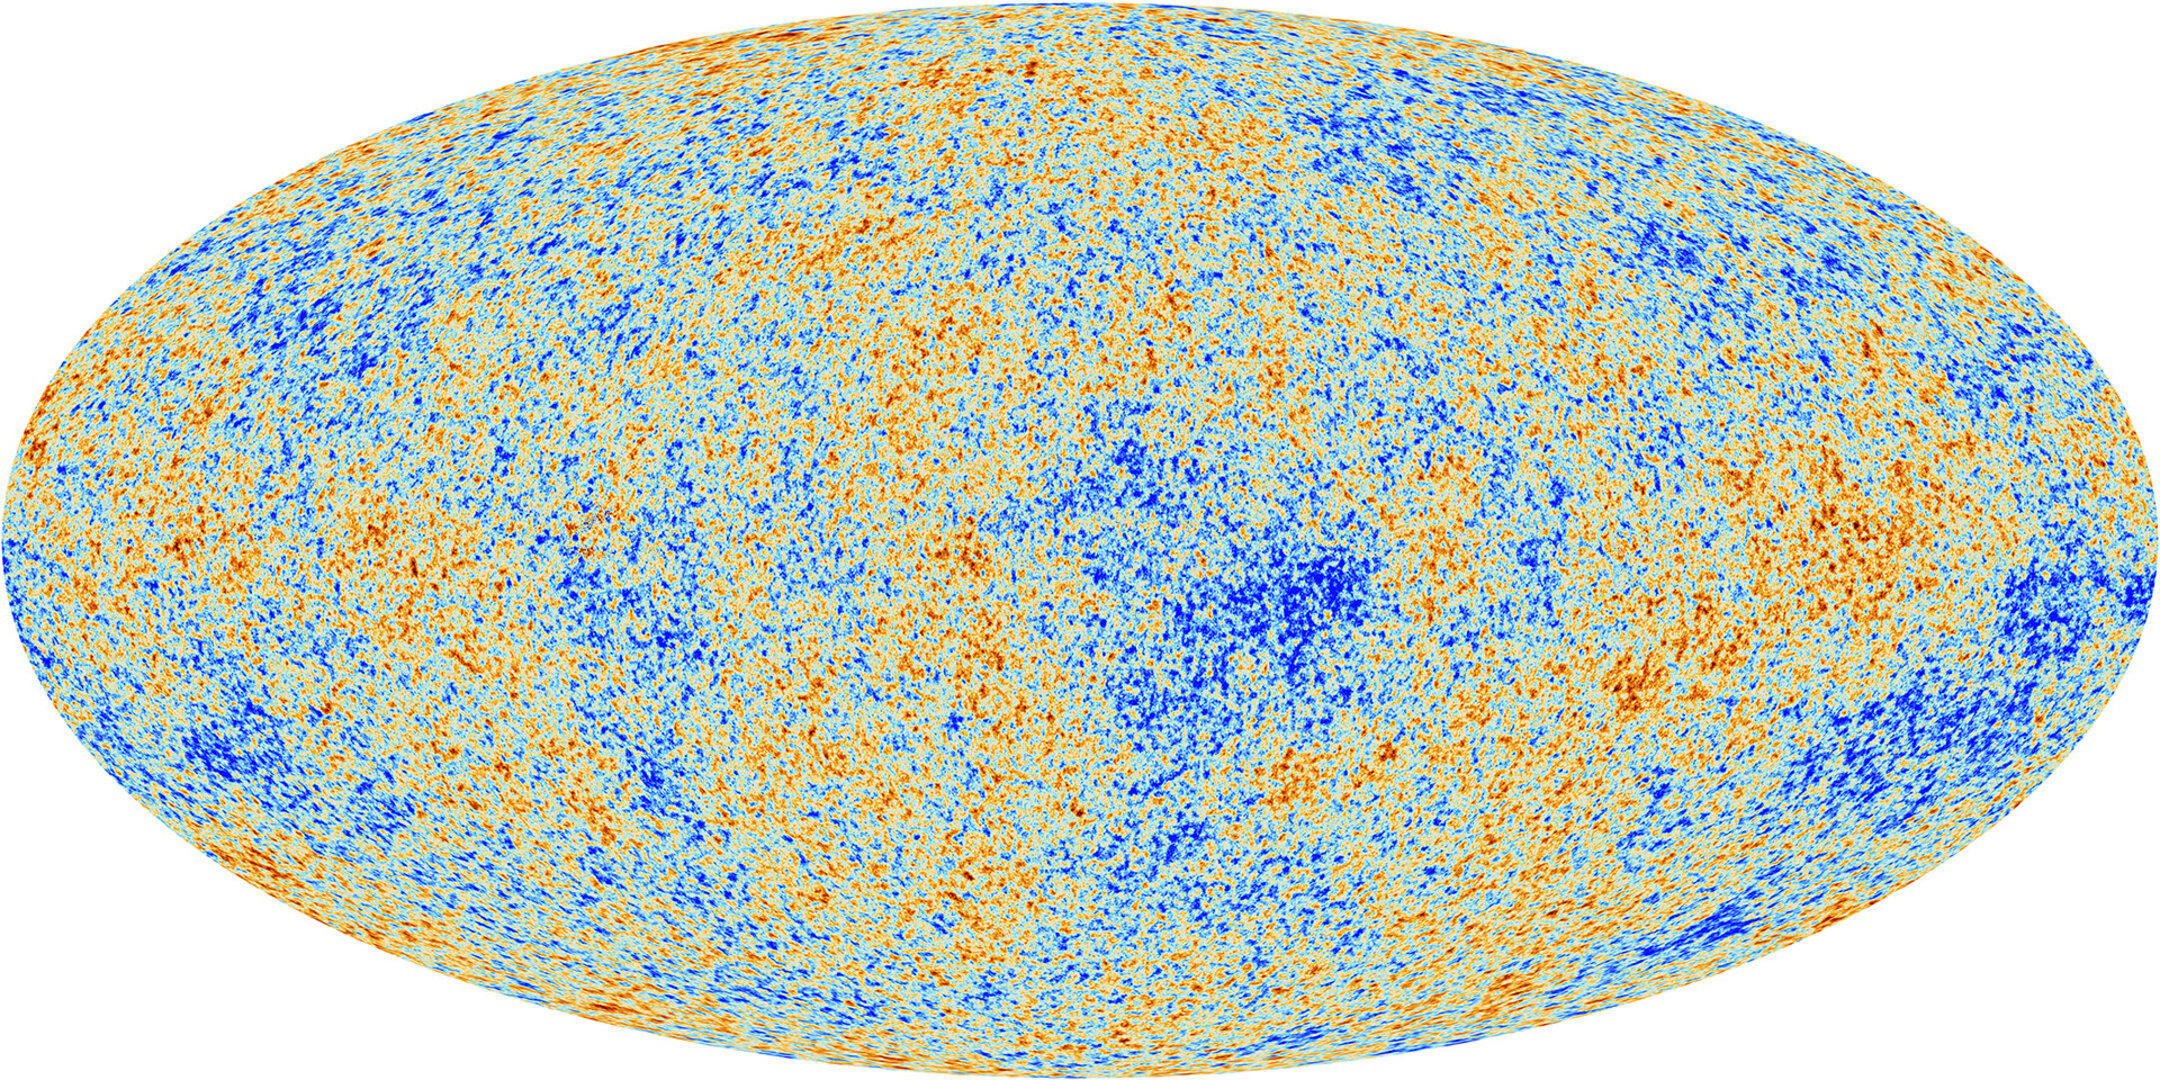
\includegraphics[width=1.\textwidth]{plots/Planck_CMB_pillars.jpg}
	\caption{Temperature fluctuations (on the scale of $10^{-5}$) of the Cosmic Microwave Background, as observed by the ESA Planck mission \citep{2016planck}.  
	}
	\label{fig:CMB}
\end{figure}


 The \textit{Cosmic Microwave Background} (CMB), discovered by Penzias and Wilson in 1965 \citep{penzias_wilson_cmb}, is the most important instance of these relics: photons decouple from the other species around 300.000 years after the Big Bang, in a process known as \textit{last scattering}, and offer us an imprint of the physical conditions of the primordial universe. The energy distribution of the CMB photons is shaped like a black body (Planck distribution):
 \begin{equation}
     I(\nu;T) = B_\nu(T) =  \frac{2h}{c^2} \frac{\nu^3}{e^{(h\nu/kT)}-1} \label{eq:black_body}
 \end{equation}
 This is expected since photons at decoupling are in thermal equilibrium, and the form of their distribution does not change as the universe expands. The temperature $T$ is strikingly uniform in the different regions of the sky: this is a strong hint in favor of the cosmological principle. However, small fluctuations at the level of $10^{-5}$ were found in the temperature distribution by the NASA COBE mission in 1992 and later described with more detail by the WMAP and Planck missions (figure \ref{fig:CMB}). These small fluctuations are one of the most important features of observational cosmology: they are considered to be the first seeds that are destined to grow into the structures we observe today in our universe. Stars, black holes, galaxies, clusters of galaxies, filaments: all of the features of the rich and complex universe we live in are thought to be originated from these small perturbations of the Cosmic Microwave Backgrounds. In the next few sections, we will explore how these perturbations grew under the influence of gravity, and eventually led to the formation of galaxies and the large-scale structure observed in the present universe.
 
 

 \subsection{Linear structure formation}
 
 The origin of the perturbations we observe in the CMB spectrum is still a matter of debate. The most reasonable and widely accepted explanation comes from the theory of \textit{cosmic inflation}. According to this theory, the universe underwent a \textit{quasi De-Sitter} phase of expansion early after the Big Bang. During this phase, quantum perturbations of the field that drove the inflationary process are turned into classical perturbations of the metric and the energy density of the universe. These classical fluctuations are directly related to the ones we measure the temperature spectrum of the CMB. 
 
 Despite the success of an inflationary mechanism in explaining many unsolved problems in cosmology, there is still no consensus on the mechanism that made the Universe inflate. Moreover, observational evidences are still lacking, allowing only a few constraints on the inflationary parameters and ruling out only a small part of the proposed models. Here, we do not investigate the inflationary theories any deeper: we assume that -- in accordance with CMB observations -- some fluctuations are present in the spatial distribution of the energy density. Our goal is to consider these perturbations as initial conditions and to study their evolution in the expanding universe. We will consider comoving coordinates, and work with the density contrast:
 \begin{equation}
    \delta(\mathbf{x}, t) = \frac{\rho(\mathbf{x},t)}{\Bar{\rho}(t)} -1 = \frac{n(\mathbf{x},t)}{\Bar{n}(t)} -1 ,
 \end{equation}
 where the quantity $\Bar{\rho}(t)$ represents the background energy density at time $t$ ($n$ stands for the numerical density).
 
 The correct way to proceed would be to consider the Einstein equations and to perform the linearization of these equations to find the correct evolution of the perturbations in curved space-time. We choose to consider here the Newtonian approximation: we work with the equations of non-relativistic hydrodynamics, coupling them with the Poisson equation for gravity. This approach holds as long as the perturbations are small in intensity as well as in scale: if these hypotheses are true, the gravitational potential is weak enough to consider valid the Newtonian regime, and the effects of the curvature of space are completely negligible. The former assumption is always valid since we consider only the regime where perturbations are small; the latter is shakier since large-scale perturbations play a relevant role in our discussion. For our purposes, it will suffice to know that the results in the Newtonian case and in the general relativistic one are completely equivalent \citep[for more details, see][]{chisari2011connection}.
 
 The hydrodynamics equations (continuity and Euler equations) for a fluid in an expanding universe in comoving coordinates $\mathbf{x}$, and subjected to the influence of a gravitational potential $\varphi(\mathbf{x})$ are ($\mathbf{v}=a\mathbf{x}$ is the peculiar velocity):
 \begin{subequations}
 \begin{align}
    \frac{\partial n}{\partial t} + 3Hn + \frac{1}{a}\mathbf{\nabla}\times(n\mathbf{v}) &= 0 \label{eq:mass_cons} \\
    a\left(\frac{\partial }{\partial t} + \frac{\mathbf{v}}{a}\times\mathbf{\nabla}\right)(Ha\mathbf{x}+\mathbf{v}) &= -\frac{1}{\rho}\mathbf{\nabla} P - \mathbf{\nabla}\varphi \label{eq:euler}
 \end{align} 
 \end{subequations}
 We have to consider also the Poisson equation for the gravitational potential, which in comoving coordinates reads:
 \begin{align}
 \mathbf{\nabla}^2 \varphi = 4\pi G \rho a^2 \label{eq:poisson}
 \end{align} 
 Expanding these relations and taking the first order of these equations in the density contrast $\delta(\mathbf{x},t)$, we are left with this system of equations:
 \begin{subequations}
 \begin{align}
    \Dot{\delta} &= - \frac{1}{a}\mathbf{\nabla}\times \mathbf{v}\label{eq:euler_linearized1}\\
    a(\Dot{\mathbf{v}}+H\mathbf{v}) &= -\frac{1}{\Bar{\rho}}\mathbf{\nabla}\delta P - \mathbf{\nabla}\delta\varphi\label{eq:euler_linearized2}\\
    \mathbf{\nabla}^2\delta\varphi &= 4\pi G\Bar{\rho}a^2\delta \label{eq:euler_linearized3}
 \end{align} 
 \end{subequations}
 The system is not closed unless we provide an equation of state for the fluid. So far, we have made no explicit assumptions on the fluid properties (however, if we were to consider radiation, the coupling between energy and the gravitational potential would be different). 
 
 At this point, however, the subtle difference between dark matter and baryons comes to play: since dark matter interacts neither with photons nor with itself -- any non-negligible self-interaction is excluded by experimental observations \citep{tulin2018dark} --, it has no pressure, hence we can completely neglect the pressure gradient term in the Euler equation (eq. \ref{eq:euler_linearized2}). Ordinary matter, on the other hand, is strongly coupled with photons until last-scattering, and it can also provide a pressure term if the temperature is not too low. This different behavior determines the fate of the two species: being pressureless, dark matter perturbations can grow under the influence of gravity without any force to oppose this growth, while ordinary matter has its own pressure -- and also the radiative pressure of photons, as long as they are coupled -- to counterbalance gravity. This means that dark matter perturbations will grow until they become non-linear well before baryonic perturbation can do the same. As soon as dark matter is sufficiently clumped, it forms gravitational wells that attract baryons. For this reason, in what follows, we analyze only the growth of dark matter perturbations. In section \ref{sec:birth_galaxies}, we will then consider baryons and analyze the competition between gravitational pull and pressure support that determines their evolution. 
 
 For a pressureless fluid, we can combine eqs. \ref{eq:euler_linearized1}--\ref{eq:euler_linearized3} in one single equation (for example, taking the time derivative of eq. \ref{eq:euler_linearized1} and the gradient of eq. \ref{eq:euler_linearized2}). We get:
 \begin{align}
    \Ddot{\delta} + 2H\Dot{\delta} = 4\pi G \Bar{\rho}\delta \label{eq:euler_growing_delta}
 \end{align}
 This is the equation of a (time-dependent) damped harmonic oscillator with an imaginary frequency. There are in general two independent solutions: a \textit{growing mode} increasing with time, and a decaying mode that does the opposite. Starting with random initial conditions, this growing mode comes to dominate the density evolution. Hence, until it becomes non-linear, the density perturbation maintains its shape in comoving coordinates and grows in proportion to a growth factor $D(t)$.
 The damping term contains the Hubble parameter, and it is therefore known as the "Hubble friction" term; it has the same role of friction in the sense that -- in comoving coordinates -- perturbations grow more slowly because of the expansion of the universe. The intensity of this damping depends on the time dependence of the Hubble factor. Tentatively, the faster the universe expands, the slower the perturbations grow with time. In turn, the expansion rate depends on the energy budget of the universe: when the universe is dominated by radiation, the scale factor is $a(t)\sim t^{1/2}$ (and therefore $H(t)=1/2t$); for a matter-dominated universe, instead, $a(t)\sim t^{2/3}$ ($H(t)=2/3t$). Since the relevant part of the growth of perturbations happens after the \textit{matter-radiation equality} (i.e., when matter took over the energy budget, approximately 100.000 years after the Big Bang), we will solve eq. \ref{eq:euler_growing_delta} using for $H(t)$ this latter dependence. 
 
 Substituting the term $4\pi G\Bar{\rho}$ in accordance with the first Friedmann equation (eq. \ref{eq:friedmann_3}) in a matter-dominated universe, eq. \ref{eq:euler_growing_delta} becomes:
 \begin{align}
    \Ddot{\delta} + \frac{4}{3t}\Dot{\delta} - \frac{2}{3t^2} \delta = 0
 \end{align}
 The growing solution can be found simply guessing a power-law solution in the form $\delta\sim t^n$:
 \begin{align}
    \delta(t) \sim D(t) \sim a \sim t^{2/3} \label{eq:growth_factor}
 \end{align}
 Therefore, perturbations will grow with this time factor until the linear approximation breaks down, and the full non-linear collapse must be followed (section \ref{sec:nonlinear_collapse}). 
 
 Note that the growth factor $D(t)$ does not depend on the scale of the perturbation: in a matter-dominated universe, small-scale and large-scale perturbations grow in the same way. This does hold in the first phase of the universe expansion, when radiation dominates over matter: because of the gravitational coupling between radiation and dark matter, \textit{super-horizon} perturbations (i.e., that have a size larger than the horizon $d_H(t) = cH^{-1}(t)$) behave differently than perturbations that are inside the horizon. For this reason, it is useful to analyze perturbations at fixed scale in the Fourier domain, defining a perturbation with scale $\mathbf{k}$ as:
 \begin{align}
    \delta_\mathbf{k}(t) = \int \d^3\mathbf{x}\, \delta(\mathbf{x},t) \,e^{-2\pi i \mathbf{k}\times\mathbf{x}}
 \end{align}
 Moreover, this approach is particularly useful as inflation theories predict perturbations given by a Gaussian random field, in which different $\mathbf{k}$-modes are statistically independent of each other. For this reason, the statistical properties of the perturbations can be described entirely by a quantity that is related to the variance of the perturbations with scale $\mathbf{k}$, known as the \textit{power spectrum} $P(\mathbf{k})$:
 \begin{align}
    \langle \delta_\mathbf{k} \delta^*_\mathbf{k'} \rangle = (2\pi)^3 \,P(k)\, \delta^{(3)}(\mathbf{k}-\mathbf{k'})
 \end{align}
 Note that the quantity $\delta^{(3)}$ is the three-dimensional Dirac delta function. According to standard models of inflation, primordial fluctuations in the energy density field have a power spectrum $P_0(k)$ following a power law of the form:
  \begin{align}
   P_0(k) \sim k^{n_s},  
  \end{align}
 where $n_s$ is determined by the inflationary parameters, but in all models it is a number close to unity (observations measure $n_s = 0.9645 \pm 0.0049$ \citep{2016planck}). 
 
 In the radiation-dominated epoch, the original inflationary power spectrum gets distorted by the different behavior of sub- and super-horizon perturbations. The resulting power spectrum is characterized by a turnover at scales of the order of the horizon at matter-radiation equality $cH^{-1}(t_\mathrm{eq})$: for larger scale, the original $k^{n_s}$ dependence is retained, while smaller scales are depressed with a factor $k^{n_s-4}$. As perturbations grow, the global amplitude of the power spectrum scales with the factor $D^2(t)$: the left panel of figure \ref{fig:power_spectrum} presents the power spectrum shape and its evolution with redshift according to the linear theory of growth. 
 
 The overall normalization factor, however, is a free parameter of the $\Lambda \mathrm{CDM}$ model, and it is usually expressed in terms of the variance of the smoothed power density field $\sigma^2(M)$. Considering the density perturbation smoothed at a scale $R$ (or equivalently at a mass $M=4\pi R^3 \Bar{\rho} /3$) has the practical purpose of determining the formation of objects at that particular scale. To apply the smoothing, we have to consider a window function $W(\mathbf{x})$: the most common choice is the spherical top-hat, for which $W=3/4\pi R^3 \Bar{\rho}$ in a sphere of radius $R$ and zero outside. With the choice of a window function, we can express the variance of density perturbations at a scale $M$ in terms of the power spectrum $P(k)$:
  \begin{align}
   \sigma^2(M) = \frac{1}{(2\pi)^2}\int \d k \, k^2\,P(k)\,\Tilde{W}(kR),  \label{eq:sigma_2_M}
  \end{align}
 where $\Tilde{W}(k)$ is the three-dimensional Fourier transform of the window function. In figure \ref{fig:power_spectrum} (right panel), we plot the variance $\sigma^2(M)$ as a function of the mass $M$ and the redshift $z$. From this plot, we can infer a fundamental property of structure formation in the $\Lambda \mathrm{CDM}$ model: since $\sigma^2(M)$ is monotonically decreasing with mass, the process of formation of collapsed structures is hierarchical (also known as "bottom-up"); first, smaller structures form out of regions where the density field is significantly larger than average, then these structures merge to form high-density regions even at larger scales. For this reason, in the next section, we will study in a simplified setting how a small-scale perturbation grows non-linear and collapses under the influence of gravity.
 
  \begin{figure}
	\centering
	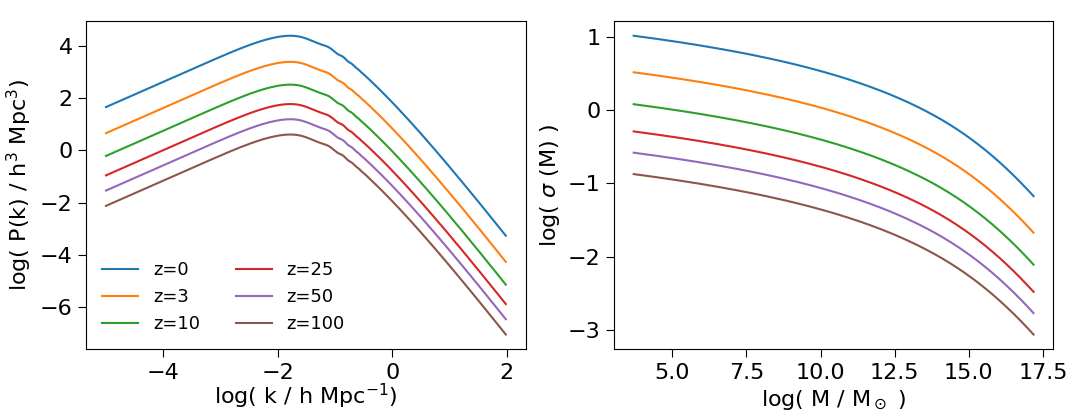
\includegraphics[width=1.0\textwidth]{plots/cosmo_1.png}
	\caption{\textit{Left}: power spectrum $P(k)$ at different redshifts $z$. At large scales (small $k$), the primordial $k^{n_s}$ dependence is retained, while at small scales (large $k$) the primordial dependence is tapered by a factor $k^{-4}$. Note that the growth with redshift is uniform in scale, as predicted by linear perturbation theory: non-linear effects such as halos formation and collapse are not considered. \textit{Right}: variance of the smoothed density perturbations at a mass scale $M$, for different redshifts $z$. The quantity $\sigma^2(M)$ can be obtained from the power spectrum $P(k)$ using eq. \ref{eq:sigma_2_M}.
	These plots were realized using the Python package \code{colossus} \citep{colossus2016}.}
	\label{fig:power_spectrum}
\end{figure}
 
 
 \subsection{Non-linear collapse} \label{sec:nonlinear_collapse}
 
 The linear approximation holds as long as perturbations are small ($\delta\ll1)$. However, perturbations are destined to leave the linear regime as they grow according to the factor $D(t)$. Describing the full, non-linear evolution of perturbations is extremely difficult: it is an N-body problem, where the gravitational interplay between all the different particles makes an analytical description of the time evolution not viable. The only general approach to the problem is to resort to numerical simulations: at every time step, the force acting on every particle is determined by computing the gravitational pull of all the other particles (usually in an approximated way). Hence, evolving every particle according to the equations of motion, the global evolution can be described with a good degree of accuracy. We will briefly elaborate on the capabilities of numerical simulations in section \ref{sec:physics_galaxies}.
 
 Here, we study the problem in a very simplified setting: we consider a matter-dominated universe, with a uniform background density $\Bar{\rho}(t)$. Within this background, we study the evolution of a single overdense blob with radius $R$ and uniform density $\rho (t) = \Bar{\rho}(t)(1+\delta(t))$. Clearly, the analytical solution we will find has very restricted applications: however, this model of "spherical collapse" is very useful to understand the properties and the distribution of structures in the universe.
 
 We start from some initial time $t_i$, and we assign to the blob a small overdensity $\delta_i$. Since structure formation interests small scale overdensities (see discussion in the last section), we can use Newtonian physics to follow the system evolution. Given the symmetry of the problem, we can think to slice the space in shells characterized by a value of the radius $r$ (considering spherical coordinates centered on the overdense sphere). Each shell will evolve independently, and -- this is the key observation -- the evolution of each shell will depend only on the shells it encloses. For this reason, there will be no "shell crossing" as the system evolves: an inner shell will never overlap with an outer one. This means that the total mass enclosed in a shell of radius $r$, $M(r)$, is constant with time. Therefore, we can integrate the equation of motion for a single shell:
 \begin{align}
   \Ddot{r} = -\frac{GM(r)}{r^2},
 \end{align}
 finding the energy conservation relation in the form:
  \begin{align}
   E = \frac{1}{2}\Dot{r}^2 - \frac{GM(r)}{r},  \label{eq:energy_collapse}
  \end{align}
  
  The energy (per unit mass) $E$ is a constant of motion, and it determines whether a given will expand forever or eventually decouple from the expansion and collapse. In fact, if $E\geq 0$, then $\Dot{r}$ will always have a positive value, hence the shell will expand forever. On the other hand, if $E<0$, then as $r$ increases, $\Dot{r}$ will eventually become negative, and the shell will stop its expansion and start to contract. 
  
  The value of $E$ can be computed at the initial time adding the kinetic energy and the gravitational potential one. Let us assume that, since $\delta_i$ is small, the original overdense region is expanding along with the background. Then the initial kinetic energy for a shell with an initial radius $r_i$ is:
  \begin{align}
   K_i = \frac{\dot{r}_i^2}{2} = \frac{H^2(t_i) r_i^2}{2},
  \end{align}
  where we have used the Hubble law $\Dot{r} = \Dot{a} r/a = Hr$. The potential energy is:
   \begin{align}
   U_i = -\frac{GM(r_i)}{r_i}
  \end{align}
  Outside the overdense region, the total mass can be approximated by $M(r_i) = 4\pi r_i^3 \Bar{\rho}(t_i)/3$, and the potential energy is therefore exactly opposite to the kinetic one:
   \begin{align}
   U_i = -\frac{H^2(t_i)r_i^2}{2}\frac{8\pi G}{3H^2(t_i)}\Bar{\rho}(t_i) = - \frac{H^2(t_i) r_i^2}{2},
  \end{align}
  where we have used the first Friedmann equation (eq. \ref{eq:friedmann_1}). Therefore, the total energy for shells outside the overdense region is zero: these shells expands indefinitely, with a time dependence (determined by integrating eq. ) $r(t)\propto t^{2/3}$. This result is expected since we have assumed that our universe is matter-dominated (Einstein-De Sitter universe).
  
  Inside the overdense region, however, things change drastically. The potential energy is now different because of the overdensity factor $\delta_i$.
  \begin{align}
   U_i = -\frac{H^2(t_i)r_i^2}{2}\frac{8\pi G}{3H^2(t_i)}\Bar{\rho}(t_i)(1+\delta_i) = - \frac{H^2(t_i) r_i^2}{2}(1+\delta_i),
  \end{align}
  Thus, the total energy density is negative, and it has a value that is proportional to the overdensity $\delta_i$:
  \begin{align}
  E = -\frac{H^2(t_i) r_i^2}{2}\delta_i
  \end{align}
  From the discussion above, we can thus conclude that any overdensity will eventually collapse. The maximum radius reached by any shell can be easily found by setting the total energy equal to the gravitational potential one:
  \begin{align}
   r_m = r_i (\delta_i^{-1} + 1)
  \end{align}
  This means that a larger overdensity will stop expanding at a smaller radius, collapsing in a shorter time. The complete time evolution of the system can be found integrating eq. \ref{eq:energy_collapse}. We are not interested in the details of this solution: it suffices to know that, as expected, every shell starts from a radius $r_i$, expands until it peaks at $r_m$, and then contracts back, finally collapsing to a single point of infinite density. Long before this happens, however, the approximations that matter is distributed spherically and random velocities are negligible break down: non-spherical motion provides gravitational collisions between particles, that become more and more frequent as density increases until collisions can bring the system in virial equilibrium in a process known as \textit{violent relaxation}.
  
  This virialization process has a fundamental importance in the history of the universe because it results in the formation of \textit{dark matter halos}. These halos provide the backbone for all the other structures we see in our universe. The halos' size and density can be easily determined by applying the virial theorem:
  \begin{equation}
    U = -2K \rightarrow E = U + K = -K 
 \end{equation}
  Knowing the total energy at the maximum radius reached by the overdensity $r_m$, the size of a collapsed halo $r_{vir}$ (\textit{virial radius}) can be found: 
  \begin{align}
    r_{vir} = \frac{r_m}{2} \approx \frac{r_i}{2\delta_i}
  \end{align}
  As for the density, it can be proven -- by using the analytical solution of eq. \ref{eq:energy_collapse} -- that halos at virialization have a fixed value for the overdensity $\delta_{vir} = 18\pi^2 -1$.
  It is also interesting to point out that, if we were to follow the linear model and to neglect the non-linear evolution completely, we would find that that, at the time corresponding to collapse, the linear growth of the overdensity would have reached a valued corresponding to $\delta_{lin}\sim 1.69$. A simplistic interpretation of this result will be very useful in the next section: we can stick to the linear growth model, and consider a halo to be formed whenever the linear overdensity reaches a value greater than $\delta_{lin}\gtrsim 1.69$.
  
  
  
  



 
 \subsection{Dark matter halos} \label{sec:halos}
 
 At the end of last section, we have introduced the virialization process, along with expressions for the virial radius $r_{vir}$ and the virial overdensity $\delta_{vir}$. Here, we explore further some fundamental properties of dark matter halos, such as their physical conditions, their abundance across cosmic time, and their radial profile. These properties will be extremely useful in predicting the behavior of baryons and the galaxy evolution process.
 
 First of all, since we know the value of the overdensity $\delta_{vir}$ at which halos form, we can express the virial radius as a function of the halo mass $M_h$ and of the redshift $z$ ($\Bar{\rho_0}$ is the average matter density of the universe today):
  \begin{align}
    r_{vir} = \sqrt[3]{\frac{3M_h}{4\pi\delta_{vir}\Bar{\rho}_{vir}}}=\sqrt[3]{\frac{3M_h}{4\pi\delta_{vir}\Bar{\rho}_0(1+z)^3}}
  \end{align}
  This relation, however, holds only for a matter-dominated universe. As dark energy plays an important role in the late-universe evolution (when dark matter halos come into play), we have to account for its effect on accelerating the universe's expansion and thus contrasting the effect of gravity. A more general formula for the virial radius $r_{vir}$ is \citep{bryan1998statistical}:
  \begin{align}
    r_{vir} = 0.784 \,\left(\frac{M}{10^8\,h^{-1}\msun}\right)\,\left(\frac{\Omega_m}{\Omega^z_m}\frac{\Delta_c}{18\pi^2}\right)^{-1/3}\,\left(\frac{1+z}{10}\right)^{-1}\,h^{-1}\,\mathrm{kpc},
  \end{align}
  where:
  \begin{align}
    \Delta_c &= 18\pi^2 + 82 (\Omega^z_m-1) - 39(\Omega^z_m-1)^2\\
    \Omega^z_m &= \frac{\Omega_m(1+z)^3}{\Omega_m(1+z)^3+\Omega_\Lambda+\Omega_k(1+z)^2}
  \end{align}
  
  From the virial radius, two other useful quantities can be defined. The first one is the circular velocity $v_c$: it describes the average Keplerian velocity of particles at the virial radius $r_{vir}$. The second one is the virial temperature $T_{vir}$, which can be defined using the average kinetic energy of particles moving at $v_c$:
  \begin{align}
    v_{c} &= \sqrt{\frac{GM_h}{r_{vir}}} = 23.4 \,\left(\frac{M}{10^8\,h^{-1}\msun}\right)^{1/3}\,\left(\frac{\Omega_m}{\Omega^z_m}\frac{\Delta_c}{18\pi^2}\right)^{1/6}\,\left(\frac{1+z}{10}\right)^{1/2}\,\kms \label{eq:circular_velocity}\\
  T_{vir} &= \frac{\mu m_p v_c^2}{2k_B} = 1.97\times10^4 \,\left(\frac{\mu}{0.6}\right)\left(\frac{M}{10^8\,h^{-1}\msun}\right)^{2/3}\,\left(\frac{\Omega_m}{\Omega^z_m}\frac{\Delta_c}{18\pi^2}\right)^{1/3}\,\left(\frac{1+z}{10}\right)\,\mathrm{K} \label{eq:virial_temperature}
  \end{align}
  In this last relation, $m_p$ is the mass of a proton, $k_B$ is the Boltzmann constant, and $\mu$ is the mean molecular weight, defined as $\mu^{-1} = m_p n/\rho$.
  The quantities here discussed will play an important role in the subsequent evolution of galaxies, as they have a critical impact on the properties of baryons bound in halos. 
  

  Another critical information we have to determine is the number density of halos through cosmic time. This quantity is known as the \textit{halo mass function} (HMF), and it is directly connected to the abundances of galaxies and galaxy clusters. To this purpose, a useful analytical formulation was first proposed by Press \& Schechter \citep{press_schechter}, and later refined by Sheth \& Tormen \citep{sheth1999large}. This Press-Schechter formalism builds its foundations on the spherical collapse model for a halo, as well as on the matter density power spectrum. Given an overdensity $\delta_M$ smoothed at scale $M$, its distribution can be determined knowing the one of the raw overdensity field $\delta$: it is a Gaussian, with a variance given by $\sigma^2(M)$ (eq. \ref{eq:sigma_2_M}). Moreover, as we have pointed out at the end of the last section, working within the linear formalism we can consider an overdensity to have already collapsed in a halo if $\delta_M$ is greater than a critical value (i.e., $\delta_c\approx1.69$). The key point here is to notice that we can equal the probability that an overdensity $\delta_M$ is greater than the threshold value $\delta_c$ to the \textit{collapsed fraction} in halos of mass greater than $M$, $f(>M,z)$ (i.e., the fraction of matter in the Universe contained inside halos of mass greater than $M$). This is because if the statistical realizations of $\delta_M$ have a value above the threshold, then they are already part of a halo of mass $M$:
  \begin{align}
    f(>M,z) = \int_{\delta_c}^\infty \d \delta_M\, \frac{1}{\sqrt{2\pi \sigma(M,z)}}\, \exp\left(-\frac{\delta_M^2}{2\sigma^2(M,z)}\right)
 \end{align}
 Recalling the growth factor $D(t)$ (eq. \ref{eq:growth_factor}), we know that $\sigma(M,z) = \sigma(M)D(z)$ (where $\sigma(M)$ is today's value and $D(z)$ is normalize to be unity at present). For this reason, we can change variables and rewrite the integral defining the critical density as a function of redshift $\Tilde{\delta}_c = \delta_c / D(z)$:
  \begin{align}
   f(>M,z) = \frac{1}{\sqrt{2\pi \sigma(M)}}\int_{\tilde{\delta}_c}^\infty \d \delta_M\, \exp\left(-\frac{\delta_M^2}{2\sigma^2(M)}\right) = \frac{1}{2}\mathrm{erfc}\left(\frac{\tilde{\delta}_c}{\sqrt{2}\sigma(M)}\right) \label{eq:collapsed_fraction}
 \end{align}
 However, there is a problem with this way of reasoning. This can be understood considering the limit $M\rightarrow0$: given the discreteness of the problem, in this limit, we should recover $f(<M,z)\rightarrow1$; instead, eq. \ref{eq:collapsed_fraction} tends to $1/2$. This is because we are missing those regions that, although they are too underdense to create a halo at a scale $M$, they still make part of halos at a larger scale $M'>M$. To account for this problem (dubbed the “cloud-in-cloud” problem), we add a global factor of $2$ to recover the correct low mass limit. Other approaches (e.g., excursion set theory \citep{excursion_set_theory}) recover this missing factor correctly.
 
 Given the collapsed fraction, we can find the mass distribution of halos (HMF) simply differentiating $f(>M,z)$ with respect to the mass $M$:
   \begin{align}
\frac{\d n(>M,z)}{\d M} = \frac{\Bar{\rho}}{M} \frac{\d f(>M,z)}{\d M} = \sqrt{\frac{2}{\pi}}\,\frac{\Bar{\rho}}{M}\,\frac{\tilde{\delta}_c(z)}{\sigma^2(M)}\,\left|\frac{\d \sigma(M)}{\d M}\right|\,\exp\left(-\frac{\tilde{\delta}^2_c(z)}{2\sigma^2(M)}\right) \label{eq:press_schechter}
 \end{align}
 In the left panel of figure \ref{fig:press_schechter_NFW}, we plot the HMF as a function of the halo mass $M$ for different redshift realizations $z$. From this plot, we can appreciate the power of the Press \& Schechter formalism: it provides a way to describe the dark matter structures growth, accounting in a statistical manner for the hierarchical clustering expected within the $\Lambda\mathrm{CDM}$ model.
 
 
 Finally, as for the density profile of dark matter halos, no analytical approach gives convincing results. The simple spherical collapse model we have considered assumes the initial density to be uniform, but makes no claims on the final virialized density. A common choice for the density profile, motivated by observations of galactic curves, is a constant power-law with slope $-2$:
   \begin{align}
    \rho(r) = \rho_{vir}\left(\frac{r_{vir}}{r}\right)^2 \label{eq:iso_sphere}
  \end{align}
  This profile, known as \textit{isothermal sphere}, has the property that the total mass enclosed in a radius $r$ is proportional to the radius itself, and hence the circular velocity (and the virial temperature) are independent of the radius, and so are the global properties of the halo. Despite giving acceptable results at large radii, the isothermal sphere is not able to account for the flattening of the profile in the inner regions of the halo.
  
  A much more accurate fit to the average halos profile was first provided by Navarro, Frenk, and White \citep{NFW_profile, NFW_profile_2} using dark matter numerical simulations. The so called "NFW profile" is shallower than an isothermal sphere in the inner region, and steeper in the outer:
  \begin{align}
    \rho(r) = \frac{\rho_{crit}\,\Delta_c}{\left(\frac{r}{r_s}\right)\left(1+\frac{r}{r_s}\right)^2}, \label{eq:nfw_profile}
  \end{align}
  where $\rho_{crit}$ is the critical density, $r_s$ is a parameter known as the "halo scale radius", and $\Delta_c$ is given by the following expression:
    \begin{align}
    \Delta_c = \frac{\delta_c}{3}\frac{c^3_N}{\ln(1+c_N)-c_N/(1+c_N)}
  \end{align}
  $\delta_c$ is the critical density based on which halos are defined: for the spherical collapse model, we have seen that $\delta_c=18\pi^2\approx177$; however, a conventional value of $\delta_c=200$ is often used. $c_N = r_{vir}/r_s$ is the \textit{concentration parameter}, and it can be expressed as a function of redshift \citep{dutton2014cold} as it reflects the critical density of the Universe at the collapse redshift. In the right panel of figure \ref{fig:press_schechter_NFW}, we plot a comparison between the isothermal sphere and the NFW profile.

\begin{figure}
	\centering
	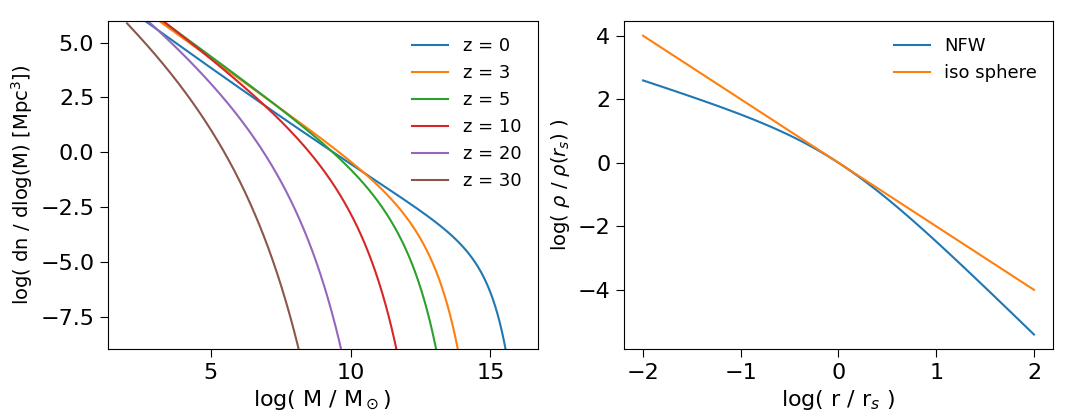
\includegraphics[width=1.0\textwidth]{plots/cosmo_3.png}
	\caption{\textit{Left}: halo mass function (number density of halos in a given mass logarithmic bin) for different redshifts $z$, according to the Press \& Schechter formalism (eq. \ref{eq:press_schechter}). The hierarchical growth of halos can be inferred from this plot, as low-mass halos are more abundant for high redshift, while higher mass halos are formed only at later redshifts. \textit{Right}: comparison between the isothermal sphere (eq.\ref{eq:iso_sphere}) and the NFW profile (eq. \ref{eq:nfw_profile}) for a dark matter halo. Radii are plotted in units of the scale radius $r_s$, while densities are divided by the density at scale radius $\rho(r_s)$. 
	}
	\label{fig:press_schechter_NFW}
    \end{figure}

\section{The first galaxies in the universe} \label{sec:birth_galaxies}


 In the basic picture we have portrayed in the last section, dark matter particles start to clump early in the primordial universe, and this process culminates with the formation of the first halos around redshift $z\sim30$. The resulting matter distribution, known as the \textit{cosmic web} because of its clumped and filamentary structure, has been confirmed by several large N-body simulations \citep[e.g.,][]{Springel:2005nw}. 
 
 However, so far we have completely ignored the fate of baryons: this is a key piece of the puzzle, as most of the information we can obtain about the universe is in the form of electromagnetic signals. Since dark matter does not interact with light, there is little hope to probe its structure and the general evolution of the universe if we do not understand how baryons evolve after they recombine and decouple from photons at last scattering. Unfortunately, these interactions with light and with themselves make baryons' behavior extremely difficult to model: unlike dark matter particles, baryons can combine in many atomic and molecular species, they can aggregate in complex structures, and cool or heat by emitting or absorbing light. 
 
 For these reasons, any predictions on their evolution involve a large number of physical processes, intertwined on a multi-scale level. In this section, we sketch the evolution of baryons as they fall into dark matter halos and form the first stars and galaxies. As these objects are created, they deeply impact the environment they are surrounded by, causing a profound modification of the global properties of the universe and finally making it similar to the one we observe today.
 
 \subsection{Jeans analysis} \label{sec:jeans}
 
 We have already introduced a (non-relativistic) description of the hydrodynamical properties of matter: mass conservation (eq. \ref{eq:mass_cons}), Euler (eq. \ref{eq:euler}) and Poisson (eq. \ref{eq:poisson}) equations are valid both for baryons and for dark matter. In the case of baryons, however, we cannot neglect the pressure term, and thus we need to relate the pressure to the density of the fluid by providing a thermodynamical closure.
 
 The most reasonable choice of closure is the adiabatic one: we assume the entropy is conserved, and thus the variations in pressure are proportional to the ones in density; the proportionality constant is the sound speed of the fluid:
 \begin{align}
   c_s^2 = \frac{\delta P}{\delta \rho} 
 \end{align}
 With this definition, we can rewrite the linear expansion of hydrodynamical equations (eqs. \ref{eq:euler_linearized1}--\ref{eq:euler_linearized3}) as:
 \begin{align}
    \Dot{\delta} &= - \frac{1}{a}\mathbf{\nabla}\times \mathbf{v}\\
    a(\Dot{\mathbf{v}}+H\mathbf{v}) &= -c_s^2\mathbf{\nabla}\delta  - \mathbf{\nabla}\delta\varphi\\
    \mathbf{\nabla}^2\delta\varphi &= 4\pi G\Bar{\rho}a^2(\delta+\delta_{dm}) 
 \end{align} 
 Note that in the Poisson equation, we have considered both the contributions from baryons and the ones from dark matter, as -- from the discussion in the last section -- dark matter perturbations are non-negligible. From this point onward, however, we will assume $\delta_{dm}=0$ and work with baryonic only perturbations: this simplistic assumption will allow us to determine some useful properties of baryons that will be important in later discussions.

 We can combine again the three hydrodynamical equations into a single one, obtaining the same result as eq. \ref{eq:euler_growing_delta} with a pressure contribution opposing the gravitational coupling:
  \begin{align}
    \Ddot{\delta} + 2H\Dot{\delta} = 4\pi G \Bar{\rho}\delta + \frac{c_s^2}{a^2} \mathbf{\nabla}^2 \delta 
 \end{align}
 The best way to deal with this kind equation is to work in the Fourier $\mathbf{k}$ domain; the Laplacian operator transforms into a $-\mathbf{k}^2$ factor, yielding:
 \begin{align}
    \Ddot{\delta}_\mathbf{k} + 2H\Dot{\delta}_\mathbf{k} + c_s^2\left( \frac{k^2}{a^2}-k_J^2\right)\delta_\mathbf{k},
    \label{eq:jeans}
 \end{align}
 where we have defined $k_J$ to be:
  \begin{align}
   k_J = \sqrt{\frac{4\pi G\Bar{\rho}}{c_s^2}}
 \end{align}
 Eq. \ref{eq:jeans} is a damped harmonic oscillator with a frequency $\omega^2=c_s^2\left( k^2/a^2-k_J^2\right)$: if the frequency is positive, the solutions are damped sines and cosines, and perturbations do not grow with time; a negative frequency, instead, corresponds to a growing solution that allows the perturbation to turn non-linear and ultimately leads to collapse (as we have already seen in the dark matter only case).
 Therefore, expressing the growth condition in terms of the \textit{Jeans scale} $\lambda_J$:
 \begin{align}
   \lambda_J = \frac{2\pi}{k_J} = \sqrt{\frac{4\pi c_s^2}{G\Bar{\rho}}}, \label{eq:jeans_scale}
 \end{align}
 we find that the overdensity at a (comoving) scale $\lambda$ collapses if the (physical) scale $a\lambda$ is greater than the Jeans scale $\lambda_J$. This condition can be well understood noting that $\lambda_J \sim c_s/\tau_{ff}$; $\tau_{ff}$ is the free-fall time, defined as:
 \begin{align}
\tau_{ff} = \frac{1}{\sqrt{G\rho}} \label{eq:free_fall}
 \end{align}
 Therefore, we are comparing the gravity timescale $\tau_{ff}$ with the time it takes pressure to act on the fluid ($a\lambda/c_s$): if the gravity timescale is short enough, information will not propagate fast enough for pressure to prevent the collapse of the structure. 
 
 We can turn the Jeans scale into a Jeans mass, in order to study which is the mass threshold for baryonic structures to collapse:
 \begin{align}
   M_J = \frac{4\pi}{3} \left(\frac{\lambda_J}{2}\right)^3\Bar{\rho} = \frac{4\pi^{5/2}}{3G^{1/2}}\Bar{\rho}_0^{-1/2}\,(c_s^2a)^{3/2},
 \end{align}
 where we have used the background density scaling $\Bar{\rho} = \Bar{\rho}_0 \,a^{-3}$. Thus, the Jeans mass evolves as the universe ages, allowing structures at different scales to collapse. In order to study this evolution, we have to determine the sound speed of baryons $c_s$. If baryons are decoupled from photons (after recombination), they can be considered as an ideal gas: thus, the adiabatic sound speed can be determined knowing that $P\rho^{-\gamma}\sim \mathrm{const.}$, with $\gamma$ being the adiabatic index ($\gamma=5/3$ for a monoatomic gas). Using the state equation for ideal gases, as well as the definition of mean molecaular weight $\mu$:
 \begin{align}
   P = nk_BT= \frac{\rho}{\mu m_p}k_B T, \label{eq:state_equation}
 \end{align}
 we find the following expression for $c_s$:
 \begin{align}
   c_s^2 =\gamma \frac{k_B}{\mu m_p} T,
 \end{align}
 The temperature of baryons, however, is not easy to determine. If baryons are moving freely along with the Hubble flow, their temperature scales as $T\propto a^{-2}$. This can be easily understood considering that $v \sim a^{-1}$, and that $k_B T \sim mv^2$. However, even after recombination, baryons are not completely free from interactions with photons. This is because a small number of electrons (and protons) are not able to form atoms before the recombination reaction gets out of equilibrium: these residual free electrons remain strongly coupled to CMB photons thanks to the relatively high cross-section of Compton scattering. The energy electrons exchange with photons is then redistributed among other baryons: this process keeps the temperature of baryons locked to the one of CMB photons down to redshift $z_t \sim 100$ \citep{barkana2005probing}. For this reason, we have to distinguish between two regimes: for $z>z_t$, the temperature of baryons is the same as the temperature of photons as the resulting Jeans mass does not depend on redshift (since $c_s^2 a \sim \mathrm{const.}$):
 \begin{align}
   M_J \approx 1.35\times 10^5 \,\msun
 \end{align}
 For $z<z_t$, instead, baryons temperature evolves independently from CMB photons, and the resulting Jeans mass depends on redshift as: 
 \begin{align}
   M_J = 5.73\times 10^3 \left(\frac{1+z}{10}\right)^{3/2} \,\msun \label{eq:jeans_threshold}
 \end{align}
 This study of the Jeans mass threshold is useful to determine the general behavior of baryons whenever gravitational collapse is involved. However, we have to keep in mind that we are completely neglecting the presence of dark matter: as dark matter halos form, their gravitational influence on baryons perturbations cannot be neglected, particularly at small scales. Therefore, in the next section, we will describe a different approach that can be used to study how baryons fall into the halos gravitational wells and form structures therein.
 

 \subsection{Baryons infall and cooling} \label{sec:infall_and_cooling}
  
  In order to study the evolution of baryons in the presence of dark matter beyond linear perturbation theory, we assume that halos have already formed, and examine how baryons can accrete into the potential wells $\varphi$ of these halos. Baryons will be attracted into these wells and will start concentrating in the inner regions of the halo until the pressure becomes high enough to counter the action of the gravitational potential $\varphi$. Ultimately, hydrostatic equilibrium can be reached:
  \begin{align}
   \mathbf{\nabla} P = -\rho \mathbf{\nabla} \varphi   
 \end{align}
  If we neglect every heat loss, then the process is adiabatic and we can relate density and pressure as $P\rho^{-\gamma}$ is conserved during the infall. The equilibrium quantities will be related to the background ones ($\Bar{P}, \Bar{\rho}$): 
  \begin{align}
   \mathbf{\nabla} \left(\frac{\rho}{\Bar{\rho}}\right)^\gamma = -\frac{\rho}{\Bar{P}} \mathbf{\nabla} \varphi = -\frac{\rho}{\Bar{\rho}} \frac{\mu m_p}{\Bar{T}} \mathbf{\nabla} \varphi,  
 \end{align}
 where we have used the state equation $\Bar{P}= (\Bar{\rho}/\mu m_p) k_B \Bar{T}$. The solution of this differential equation (with the background values as boundary conditions at infinity) is:
 \begin{align}
   \rho = \Bar{\rho} \left(1-\frac{2}{5}\frac{\mu m_p}{k_B \Bar{T}}\varphi\right)^{3/2} = \Bar{\rho} \left(1+\frac{4}{5}\frac{T_{vir}}{\Bar{T}}\right)^{3/2} \label{eq:baryon_accretion}
 \end{align}
 Note that the definition of the virial temperature $T_{vir}=-\mu m_p \varphi / 2 k_B$ is only approximately compatible with expression \ref{eq:virial_temperature}, as the relation between $\phi$ and the circular velocity $v_c$ depends on the specific shape of the halo density profile.
 
 In analogy with dark matter collapse, we can set a threshold value $\delta = \rho/\Bar{\rho} -1 > \Delta_c$ for baryons overdensities to be considered as collapsed structures. We choose $\Delta_c =100$: in this way, we can find the minimum virial temperature of a halo for it to accrete a relevant amount of baryons in its core. Eq. \ref{eq:baryon_accretion} gives the condition $T_{vir} \gtrsim 25 \Bar{T}$. We already determined the evolution of the baryons temperature for $z<z_t$, finding the scaling $T\sim a^{-2}\sim (1+z)^2$. We can also write the virial temperature in terms of the virial mass (eq. \ref{eq:virial_temperature}), in order to obtain a condition on the halo masses. We find:
  \begin{align}
    M > 8\times10^3 \left(\frac{1+z}{10}\right)^{3/2}\,\msun 
  \end{align}
 Therefore, we obtain that baryons accrete on halos with masses larger than a threshold which scales with redshift as $(1+z)^{3/2}$. Note that this result is quantitatively similar to the one we have obtained using Jeans analysis (eq. \ref{eq:jeans_threshold}): therefore, we can express this condition as $M>M_J(z)$. Of course, both approaches found on very coarse -- although different -- approximations, but they are aligned in suggesting a value of the mass scale for which baryons are actually able to clump and subsequently form complex structures. As halos formation proceed hierarchically (sec. \ref{sec:halos}), the presence of such a threshold suggests that baryons will start clumping in structures with $M\sim M_J(z)$, as soon as these halos are numerous in the universe. 
 
 As (quasi-)hydrodynamical equilibrium is reached, baryons form a self-gravitating structure where pressure prevents further collapse within the halo. The baryons' temperature at this point is comparable to $T_{vir}$, as the gas gets gravitationally heated during the infall. However, this state of equilibrium can be easily disrupted as baryons, unlike dark matter, can radiate away thermal energy: this key process explains how smaller structures such as stars and black holes form within the halo. The loss of energy, in fact, results in a loss of pressure support, and thus the gas has to contract to higher densities for it to be effective again.
 
 The \textit{radiative cooling} processes mentioned here will play a major role in the next chapters and will be thoroughly analyzed in chapter \ref{chap:model}. In this discussion, we just note how the efficiency of cooling (in the low-density regime) depends both on the gas temperature and on its composition. As primordial gas contains a negligible amount of metals (i.e., elements heavier than helium), cooling can only happen through lines excitation of hydrogen and helium. This poses a problem, however, as these cooling channels are not effective below $T\sim10^4\,\mathrm{K}$. This temperature corresponds to a virial mass of $M_{vir}\sim 10^8\,\msun$ at $z=10$: this would set a very high threshold for fragmentation to happen within the halo, and subsequently, delay star formation until lower redshifts. It turns out, though, that another cooling channel can open up at a temperature of $T\sim 10^3\,\mathrm{K}$ due to the rotational-vibrational transitions of $\mathrm{H}_2$ molecules. This channel sets a lower threshold for baryons' temperature to result in sufficient cooling. However, $\mathrm{H}_2$ is not always present: even a small amount of UV radiation in the \textit{Lyman-Werner (LW) band} ($10.2-13.6\,\mathrm{eV}$) can dissociate the molecule in a two-step photo-dissociation mechanism known as \textit{Solomon process} \citep{draine_bertoldi} (see also \ref{sec:radiation_fields}).
 
 For this reason, baryons' collapse in the inner regions of dark matter halos is usually described as a two-fold process: first, baryons cool down via molecular transitions in halos with a virial mass around $M_{vir}\sim10^6\,\msun$ (known as \textit{minihalos}). As the first stars form and emit UV radiation (see next section), $\mathrm{H}_2$ stops playing a major role as a coolant and galaxy formation is delayed until baryons in more massive halos ($T_{vir}\sim10^4\,\mathrm{K}$ and $M_{vir}\sim 10^8\,\msun$) emit $\mathrm{Ly}\alpha$ radiation via collisional excitation of hydrogen atoms.
 

 
 \subsection{First light and reionization} \label{sec:first_lights_reionization}
 
 Once the gas cools and loses pressure support, it collapses in the inner regions of the halo until it is supported by its angular momentum. The resulting self-gravitating structure resembles a rotating disk: a protogalaxy has formed. At this point, the gas tends to become self-gravitating (i.e., dominated by its own gravity rather than that of the dark matter). Even though the gravitational influence of the halo is still important to determine the global evolution of the galaxy, its role becomes secondary on a local level. Therefore, Jeans analysis (sec. \ref{sec:jeans}) can be applied to study further collapse and fragmentation of gas. 
 
 Fragmentation occurs at scales comparable with the Jeans scale $\lambda_J$ (eq. \ref{eq:jeans_scale}). If the cooling timescale is smaller than the dynamical one (i.e, the free-fall time $\tau_{ff}$) then the gas evolution can be considered isothermal because the energy loss is primarily compensated by an increase in density. For a constant temperature, however, the Jeans mass scales as $\rho^{-1/2}$: for this reason, as the density increases, the Jeans mass decreases, and the gas breaks up into even smaller clumps. This process leads to the formation of \textit{Giant Molecular Clouds} (GMCs). GMCs can have very different properties, as they ultimately arise from the complex interplay of cooling, gravity, turbulence, and magnetic effects: their density ranges from $10^2\,\mathrm{cm}^{-3}$ in the external regions to $10^7\,\mathrm{cm}^{-3}$ in the densest cores. In these cores, gas can ultimately collapse and reach the extreme densities necessary to ignite nuclear fusion, forming the first protostars. Note, however, that the mechanism in which stars are formed is extremely difficult to model, and many of its details are still poorly understood.
 
 %in galaxy formation models, star formation is usually implemented using some kind of prescription on the physical conditions gas has to reach in order to form a star, as well as on the efficiency of this formation process. 
 
 The birth of the first stars in the universe marks a key passage in its evolution: it is the end of the \textit{Dark Ages}. From the epoch of recombination, in fact, the universe is filled with neutral gas with a primordial composition (i.e., hydrogen, helium, and traces of metals). The properties of this gas are quite uninteresting from an astrophysical perspective: aside from the H (and $^3$He) hyperfine transition line, no electromagnetic radiation is emitted by this neutral gas. Therefore, the growth of perturbations, the formation of dark matter halos, and the collapse of baryons happen in an overall dark universe. As the first stars shine, everything changes: photons travel again in the universe, interacting with the neutral hydrogen, and, in principle, reaching our telescopes -- although we still lack the technical capabilities to observe the light emitted from first stars \citep{rydberg2013detection}. 
 
 The interaction between photons emitted by the first stars -- known as \textit{PopIII stars} -- and hydrogen atoms has a huge impact on the properties of the entire universe: photons are able to ionize the Inter-Galactic Medium (IGM), i.e., the reservoir of neutral gas that does not belong to collapsed structures and fills the universe since recombination.
 In order to appreciate the relevance of this process, we can consider the efficiency of hydrogen nuclear fusion. The energy liberated per hydrogen atom is approximately:
 \begin{align}
   E = 0.7\% \,m_p c^2 \approx 6\times 10^6\,\mathrm{eV}
 \end{align}
 As it takes only $13.6 \,\mathrm{eV}$ to ionize an hydrogen atom, it suffices to convert into stars a small fraction (around $10^{-5}$) of neutral gas to ionize it all. This process is known as \textit{reionization}, and it represents the last phase transition that the universe undergoes in its history. Current models place the Epoch of Reionization (i.e., the time at which the universe is fully ionized) around $z\sim6-7$ \citep{mesinger_2016}.
 
 Reionization is a complex process, as it is directly influenced by the physics of structure formation on a multi-scale level: ionization fronts travel from single stars to intergalactic distances. We can sketch the process using a simple analytical model as follows: we consider a single, star-forming galaxy surrounded by a neutral IGM. As ionizing photons are emitted by the galaxy, they travel freely until they find the boundary between the neutral and ionized gas: ultimately, they are able to drive an ionization front that travels further into the IGM. The size $R_i$ of the resulting \HII (i.e., ionized hydrogen) region changes according to the following relation:
 \begin{align}
   \langle n_\mathrm{H}\rangle 4\pi R_i^2 \frac{\d R_i}{\d t} = \dot{N}_\gamma- \alpha \langle n_\mathrm{H}^2\rangle \frac{4\pi}{3} R_i^3
  \end{align}
  In this formula, the velocity of the ionizing front depends on the total rate of ionizing photons emitted by the central galaxy $\dot{N}_\gamma$, as well as on the rate of hydrogen recombination (which causes the ionization fraction to decrease and thus slows down the shell growth). The former term can be written as:
  \begin{align}
  \dot{N}_\gamma = \frac{\d}{\d t}\left(\fesc\, N_b\, f_*\, N_{\gamma,b}\right) \approx  \fesc \, f_*\, N_{\gamma,b}\,\frac{\d N_b}{\d t}
  \end{align}
  Here, $\fesc$ is the \textit{escape fraction} (i.e., the fraction of ionizing photons that are able to escape from the galaxy), $N_b \,f_*$ is the total number of baryons in stars, and $N_{\gamma,b}$ is the rate of photons emitted by a single stellar baryon. The second equality follows if we assume that only the total number of baryons inside the galaxy $N_b$ changes significantly over time: this approximation neglects the changes in the properties of stellar population, feedback, and galaxy's morphology, and thus, it is valid only for a very coarse model. Introducing also the clumping factor $C= \langle n_\mathrm{H}^2\rangle/  \langle n_\mathrm{H}\rangle^2  $, we can rewrite the equation describing the evolution of the ionized volume $V_i$ as:
  \begin{align}
   \dot{V}_i = \langle n_\mathrm{H}\rangle^{-1} \,\fesc \, f_*\, N_{\gamma,b}\,\dot{N}_b - \alpha C \langle n_\mathrm{H}\rangle\,V_i \label{eq:volume_reionization}
  \end{align}
  Considering the global picture, at the Epoch of Reionization the universe will be filled by these expanding ionized regions that eventually overlap and merge creating larger \HII structures until the whole IGM becomes ionized. We can compute the filling factor of \HII regions, $Q_i$, by summing over many ionized volumes and dividing by the total volume of the universe $Q_i = \sum_i V_i / V_\mathrm{tot}$. The equation governing the evolution of $Q_i$ follows directly from eq. \ref{eq:volume_reionization}:
   \begin{align}
   \frac{\d Q_i}{\d t} = \fesc \, f_*\, N_{\gamma,b}\,\frac{\d f(>M_\mathrm{min},z)}{\d t} - \alpha C \langle n_\mathrm{H}\rangle\,Q_i, \label{eq:reionization_equation}
  \end{align}
  where we have rewritten the fraction of baryons collapsed in galaxies, $\sum_i N_{b,i}/(\langle n_\mathrm{H}\rangle\,V_\mathrm{tot})$, using the collapsed fraction of dark matter particles (eq. \ref{eq:collapsed_fraction}) in halos with masses larger than a threshold value $M_\mathrm{min}$ (see discussion in section \ref{sec:infall_and_cooling} for more details). 
  
  The picture here presented describes the main features of reionization in a very sketchy way. A more detailed treatment is possible using numerical/statistical techniques \citep[e.g.,][]{mesinger_2016}. However, these simple arguments are useful as they allow us to determine the key parameters that steer the evolution of $Q_i$. $f_*$ and $N_{\gamma, b}$ are connected with star formation, as they describe the efficiency of SF and the properties of stellar radiation respectively; we will deal with these parameters in section \ref{sec:star_formation}. 
  
  The two other arbitrary parameters we have introduced are the escape fraction $\fesc$ and the clumping factor $C$. These are particularly important as, depending on the detailed internal structures of the first galaxies and on their surroundings, they are largely unconstrained by observations. In particular, the escape fraction directly depends on the morphology and the distribution of column densities in the inner regions of galaxies, as ionizing photons are mainly absorbed by the neutral and dusty ISM. Both observations in the FUV band and numerical simulations (see below) are used to pinpoint the value of $\fesc$. 
  However, no consensus has been reached yet, as even the order of magnitude of $\fesc$ and its trends with mass, luminosity, and redshift are still to be established. A number of different works have tried to infer $\fesc$ from observations, obtaining values ranging between $\fesc \approx 1\,\%$ and $\fesc \approx 20\,\%$ \citep[e.g.,][]{inoue2006escape}. However, these numbers depend on a few underlying assumptions (e.g., star formation history, IGM absorption along the line of sight, absence of spurious contamination) that are difficult to benchmark. Simulations find values of $\fesc$ that tend to decrease with mass - as a consequence of a denser and more clumped ISM - and to increase with redshift. Reported values are $\fesc \approx 0.15- 0.6$ for $M_{vir}\lesssim 10^{6-7}\,\msun$, $\fesc \approx 0.05 -0.4$ for $M_{vir}\lesssim 10^{8-9}\,\msun$, $\fesc\approx 0.01- 0.07$ for $M_{vir}\sim 10^{10-11}\,\msun$ \citep{xu2016galaxy,wise2014birth, ma2020no}. However, other authors find much lower values for $\fesc$, as low as $10^{-5}$ \citep{paardekooper2015first}.
  The discussion on the relevance of the escape fraction in determining the characteristics of reionization is particularly interesting in the context of our thesis work, as $\fesc$ will play an important role in our model (chapter \ref{chap:model}).
 
 
 
 

\section{Basic physics in galaxy evolution} \label{sec:physics_galaxies}
  


 In the last section, we have outlined the process of galaxy formation and its direct implications on the universe's evolution. Here, we face the problem of studying galaxies as they evolve with the universe. This is an extremely complex task, because galaxy evolution is led by the interplay of many different processes at different scales and levels. 
 
 There exist different techniques that have succeeded in describing how galaxies evolve with time, matching observable quantities such as luminosity functions (LFs), chemical compositions, and density distributions. Numerical simulations are the most explicit way to model the formation and evolution of galaxies in a subset of a virtual universe whose initial conditions are set to match real observations. The basic idea is to solve numerically the equations for gravity, hydrodynamics, thermodynamics, and chemistry, using particles and/or grid cells that represent dark matter, gas, and stars. Even though their resolution and their spatial extension are limited by computational exigencies, these simulations can capture the intrinsic complexity of a variety of different physical processes. Small-scale processes (e.g., star formation) are implemented using effective prescription and parameters that are fine-tuned to match observations. A few years ago, many different simulations have finally succeeded in reproducing galaxies that are statistically compatible with the ones we observe in the local universe (see Figure \ref{fig:eagle}). 
 
 A different approach one can take in order to follow galaxies' evolution is represented by "\textit{Semi-Analytic Models}" (SAMs).  This method focuses on a set of simplified equations that describe the mutual interactions between different components (e.g., inflowing gas, outflowing gas, stars, cool ISM) via some parameters that are tuned according to observations (just as numerical simulations). The growth of halos and galaxies is followed using a \textit{merger tree}, i.e., treated in a statistical way adopting a prescription such as the Press-Schechter (eq. \ref{eq:press_schechter}).

 In the next few paragraphs, we give rudimentary physical insights into the main factors that are thought to dominate the galactic evolution process: cosmological gas accretion, star formation, and feedback processes. These are included both in SAMS and in cosmological simulations, and concur to determine how a galaxy grows with time, forming new stars and increasing its size and mass content, as well as changing its global observable properties. 
 
 
\begin{figure}
	\centering
	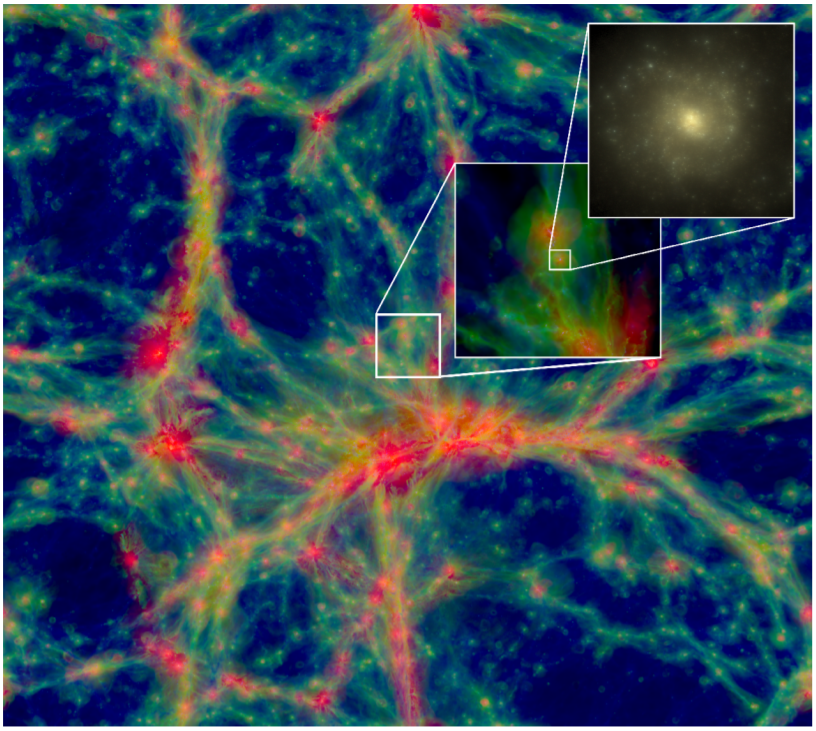
\includegraphics[width=0.57\textwidth]{plots/eagle.PNG}
	\caption{A snapshot of 100 × 100 × 20 cMpc (comoving-Mpc) taken from the EAGLE cosmological simulation \citep{schaye2015} at $z=0$. The intensity represents the gas density, while the color codes the gas temperatures from cool gas (blue) to the hotter one (red). The insets zoom on a region where a MW-like galaxy resides. 
	}
	\label{fig:eagle}
    \end{figure}
    
    
  \subsection{Gas accretion} \label{sec:accretion}
  
  Gas accretion is important to determine the evolution of the galaxy because, as stars form, they consume the cold gas reservoir inside the galaxy. Accretion from the IGM renovates this reservoir by providing new gas that can fuel the process of star formation. Therefore, the rate at which the gas accretes to the galaxy directly affects its gaseous and stellar content. 
  
  We have already described how baryons are attracted into the potential wells of dark matter halo, and form a quasi-hydrostatic hot gaseous halo that starts to cool down radiatively if the virial temperature is above a certain threshold (section \ref{sec:infall_and_cooling}). This process is responsible for galaxy formation, but it continues to provide new cold gas to the galaxy along the entire evolution process. 
  
  We can refine our discussion on gas accretion and cooling by introducing the gas cooling time $\tau_\Lambda$:
  \begin{align}
   \tau_\Lambda(r) = \frac{E_{in}}{n\,\Lambda(T)} = \frac{1}{\gamma - 1}\frac{\mu m_p k_B T}{\rho(r)\Lambda^\mathrm{(cool)}(T)} \label{eq:tcool}
  \end{align}
  $E_{in}= k_B T/(\gamma-1)$ is the internal energy of the gas, while $\Lambda^\mathrm{(cool)}(T)$ is the cooling rate (measured in $[\mathrm{erg}\,\mathrm{cm}^3\,\mathrm{s}^{-1}]$). These quantities will be explored in details in chapters \ref{chap:outflows}--\ref{chap:model}, as they constitute the building blocks of the model presented by this work. 
  
  Comparing the cooling time $\tau_\Lambda$ with the free-fall time $\tau_{ff}$ (eq. \ref{eq:free_fall}), we find a cooling radius $r_{cool}$ for which $\tau_\Lambda(r_{cool})=\tau_{ff}(r_{cool})$. Given the density dependency of these two time scalings, in the region inside $r_{cool}$ the gas cools effectively -- as its cooling time is shorter than the free-fall one --, while in the outer region dynamical effects prevail over cooling -- as the free-fall time gets shorter. Provided that a hot gaseous halo has formed as described in sec. \ref{sec:infall_and_cooling}, the gas will start cooling for $r<r_{cool}$. Therefore, we can write the accretion rate $\Dot{M}_{acc}$ as:
  \begin{align}
   \dot{M}_{acc} \sim 4\pi \rho(r_{cool})\frac{\d r_{cool}}{\d t}
  \end{align}
  In this picture, the gas is slowly accreted from the hot halo reservoir as the cooling threshold moves outside from the center. This is commonly known as "hot accretion mode".
  
  However, if the cooling radius is greater than the virial radius $r_{vir}$, then cooling is always efficient: no halo formation takes place, as the gas can cool efficiently and fall directly in the inner regions of the halo. The accretion rate, in this latter case, is only bounded by the dynamical timescale: for this reason, it is common to model this process assuming that the gas can flow into the halo on a free-fall time. The gas mass, in turn, depends on the halo mass, as the gas is accreted along with dark matter. These "cold modes" of accretion are much more efficient at providing cold, ready-to-use gas to the galaxy. For this reason, they are thought to play a major role in governing the cold gas mass budget of the galaxy, particularly at higher redshifts. As cosmological hydrodynamical simulations have shown, these modes occur along dense and cold filaments \citep{kerevs2005galaxies}, reflecting the filamentary structure of the dark matter "cosmic web" (e.g., see figure \ref{fig:eagle}). 

  As a final note, we point out that accretion is not the only way in which galaxies increase their gas reservoir. Along with their dark matter halo host, in fact, galaxies can merge and form more massive systems, in a hierarchical process that leads to galaxy growth with cosmic time. Mergers happen as a result of close encounters between different structures, and thus are more frequent as the density of objects increases. For this reason, they are thought to play an important role in driving galaxy mass growth at higher redshifts, as well as in galaxy groups and clusters. Besides increasing galaxy masses and providing new gas reservoirs, mergers are also important because they can trigger star formation as they create shocks in the gas that locally increase its density \citep{conselice_mergers}. 

  \subsection{Star formation and its consequences} \label{sec:star_formation}

  As described in section \ref{sec:first_lights_reionization}, the first stars in the universe formed out of the coldest and densest regions in Giant Molecular Clouds. These first structures -- named \textit{PopIII stars} -- are thought to have very different properties compared to the stars we observe in the local universe: they are more massive, more luminous, hotter, and metal-free \citep{haemmerle2020formation}. 
  
  These properties have important consequences: first of all, massive and luminous stars have a higher effective temperature. For this reason, the spectrum of these stars contains a larger fraction of ionizing photons (with energies greater than $13.6\,\mathrm{eV}$) as well as a greater number of photons in the LW band ($10.2-13.6\,\mathrm{eV}$). We have already discussed (sec. \ref{sec:infall_and_cooling}--\ref{sec:first_lights_reionization}) how these photons impact the galactic environment and the universe as a whole: they start the process of cosmic Reionization by creating ionizing bubbles in their surrounding medium, and they photo-dissociate $\mathrm{H}_2$ molecules hampering gas cooling in lower mass halos. Ultimately, radiation from these stars contributes to forming a background of UV photons that affects the properties of the Inter- and Circum-Galactic Media (IGM/CGM) by photo-heating and photo-ionizing the gas. The UV background (UVB) will play a critical role in our model, and we will study in detail its effects in section \ref{sec:radiation_fields}. 
  
  Another important characteristic of PopIII stars is their brief lifetime. Since the available energy for nuclear fusion is proportional to the stellar mass $M$, the stellar lifetime $\tau_s$ scales as:
  \begin{align}
      \tau_s \sim \frac{Mc^2}{L} \sim M^{-5/2},
  \end{align}
  where we have used the mass-luminosity relation $L\sim M^{7/2}$ for massive stars \citep{griffiths88}. Thus, massive stars consume their energy reserve faster and they soon run out of fuel. For a star of about $\sim 10\,\msun$, this lifetime is around tens of Myrs: this is much shorter than the dynamical timescale of the galaxy. For this reason, as the galaxy evolves dynamically, many stars form and die. The death of a massive star culminates with the collapse of the star's core: this results in a catastrophic explosion followed by shock waves propagating into the surrounding gas \citep{ostriker_supernovae} -- this phenomenon is known as Supernova (SN). Energy is injected in the Inter-Stellar Medium (ISM) by the interaction of the expanding shell with the surrounding gas. The amount of energy a single supernova can liberate is astounding: in low-mass halos, it can be greater than the gravitational binding energy of the gas. For this reason, supernovae events exert a profound influence on the life of the host halo: they can launch powerful outflows that drive gas out into the IGM, competing with the gas accretion process in determining the ISM mass budget. 
  
  Moreover, the core-collapse of a massive star often results in the formation of a remnant object, that can be either a \textit{neutron star} or a \textit{black hole}. Black holes forming out of the first stars are particularly interesting, as they are one of the candidates to be the seeds of the Super-Massive Black Holes (SMBHs) we observe today in virtually any galaxy with a central bulge \citep{Latif:2016qau}. Along with stars, SMBHs are considered to be the primary cause for driving galaxies growth: a tight correlation is in fact found between the properties of SMBHs and the ones of the galactic inner regions, strongly suggesting an interconnected coevolution process \citep{Kormendy:2013dxa}. The most straightforward way in which SMBHs couple with their host galaxies is through the energy released in their active phase of accretion: as gas falls within the black holes' potential well, it is heated to extremely high temperatures and it radiates away a considerable fraction of its binding energy. The efficiency of this process is extremely high: on average, it is an order of magnitude greater than the efficiency of Hydrogen nuclear fusion. SMBHs in their active phase are known as \textit{Active Galactic Nuclei} (AGN) -- or equivalently as \textit{Quasars} (QSOs).    
  
  Finally, the death of a massive star has another important consequence: the external layers of the star are ejected out and they mix with the cold ISM. In this way, the gas is enriched with the metal elements formed inside the star thanks to nuclear fusion. Gas exchange between galaxies and their surroundings is then responsible for bringing metals into the IGM, ultimately polluting the primordial gas everywhere in the universe (chapters \ref{chap:results}--\ref{chap:conclusion}). The process of metal enrichment has a dramatic impact on subsequent stellar evolution, as it marks the end of metal-free (PopIII) star formation. Metals such as carbon and oxygen, in fact, allow the gas to cool well below the hydrogen threshold of $10^4\,\mathrm{K}$ (section \ref{sec:cooling}): lower temperatures result in stronger fragmentation and clumping, ultimately leading to a new generation of \textit{PopII stars} characterized by lower masses and higher metallicities (i.e., mass fraction of metals in the gas). Studies show that the transition between PopIII and PopII stars happens when a metallicity threshold $Z_{crit}\sim 10^{-3.5}-10^{-5}$ is reached \citep{bromm2001fragmentation}. This value is relatively low, as in $M_{vir}\sim10^8\,\msun$ halos, it can be attained thanks to the metal yields of a few SNe explosions \citep{karlsson2008uncovering}.
  
  Globally, star formation depends on the availability of cold gas in the ISM. A possible parametrization for the star formation rate (SFR) in a galaxy is:
  \begin{align}
    \mathrm{SFR}(t) = \dot{M}_\mathrm{star} = f_* \,\dot{M}_{acc}(t) \label{eq:feedback_parameter}
  \end{align}
  The parameter $f_*$ expresses the role of \textit{feedback mechanisms} acting on the gas: these are the subject of the next section.
  Note that, in this relation, we have assumed that the gas contributes to forming stars as soon as it is accreted in the ISM. We should caution that this assumption is not true in general: the exact link between accretion and star formation is still to be established, as both observations and theoretical arguments struggle to explain this connection in detail \citep[e.g.,][]{almeida2016}. This problem can be mitigated by considering more sophisticated prescriptions for star formation (e.g., defining a time distribution for the probability of forming stars after accretion). 
  
  Once a star formation rate history $\mathrm{SFR}(t)$ has been established, one can describe the evolution of a stellar population in a galaxy by assuming an Initial Mass Function (IMF) (i.e., the initial probability of forming a star of mass $m$). Common choices for PopII stars IMFs include (broken) power laws of the form $\Phi(m) \propto m^{-\alpha}$ (e.g., $\alpha = -2.35$ for the Salpeter IMF \citep{salpeter1955}). Knowing the spectral emission for a single star $f_\mathrm{star}(t,Z)$ as a function of time $t$ and metallicity $Z$, then, it is possible to sum the light emitted from all the stellar sources at a time $t$ to come up with a prediction for the spectral emission of a galaxy. This can then be compared to observations in order to assess the validity of the assumptions made in the model; this approach is known as \textit{Stellar Population Synthesis} (SPS). The final spectrum at a given time $t$, $f_\mathrm{CSP}(t)$, will read:
  \begin{align}
    f_\mathrm{CSP}(t) = \int_{0}^{t} \int_{0}^{Z_\mathrm{max}}\int_{m_\mathrm{min}}^{m_\mathrm{max}(t)} \mathrm{SFR}(t-t')\,P(Z; t-t')\,\Phi(M)\, f_\mathrm{star}(t',Z) \,e^{-\tau_d(t')}\,\d t'\,\d Z\,\d M \label{eq:galaxy_spectrum}
  \end{align}
  where $Z_\mathrm{max}$, $m_\mathrm{min/max}$ are the extremal values for the metallicity and the stellar masses respectively, and $P(Z;t)$ is the time-dependent metallicity distribution. The negative exponential term accounts for dust attenuation: $\tau_d$ is the averaged dust optical depth in the galaxy, obtained integrating the dust absorption coefficient $\alpha_d$ along different line of sights (LOS).
  
  \begin{figure}
	\centering
	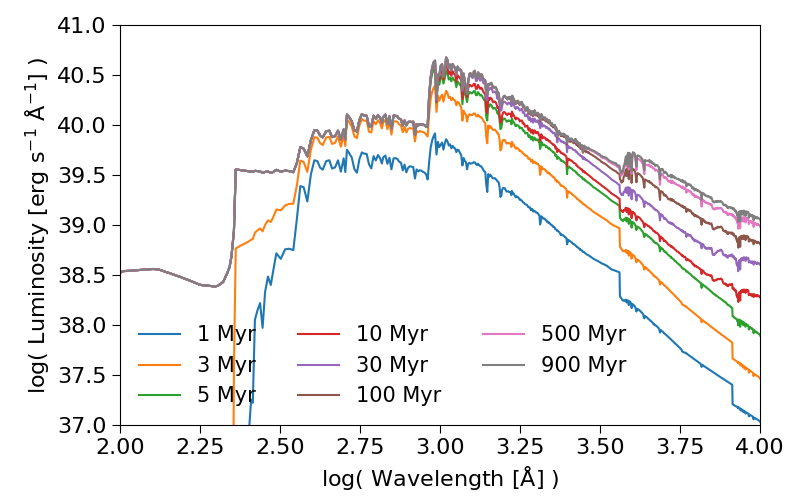
\includegraphics[width=0.6\textwidth]{plots/starburst99.PNG}
	\caption{Luminosity of a galaxy as a function of the wavelength, created using the Stellar Population Synthesis code \code{starburst99} \citep{leitherer1999}. The different curves refer to different galactic evolutionary times (between $1\,\mathrm{Myr}$ and $1\,\mathrm{Gyr}$). The galaxy has a SFR $=1\,\msun$, a metallicity $Z=0.040$; the IMF is taken to be Salpeter-like with a lower mass threshold of $1\,\msun$ and a higher mass threshold of $100\,\msun$.
	}
	\label{fig:scp}
    \end{figure}
    
  Figure \ref{fig:scp} represents an instance of these spectra for different time snapshots, created using the SPS code \code{starburst99} \citep{leitherer1999}. These spectra are generally peaked in the UV - where the light from the youngest and brightest stars is concentrated - and they decrease in intensity as the wavelength increases. However, this general behavior does not include the contribution of dust. In fact, dust absorbs radiation and thus heats up to hundreds of Kelvin, emitting thermal radiation in the IR. In order to account for this radiation, a second term has to be added inside the integral in eq. \ref{eq:galaxy_spectrum}.
  

  \subsection{Feedback and the baryon cycle} \label{sec:feedback}
  
  
  We have already examined how the birth of PopIII stars influences the environment in which they live. These are all instances of feedback mechanisms: the term feedback refers to the fact that the birth of a star has a relevant impact on the subsequent rate (and properties) of star formation itself. In a broader sense, feedback is the expression of the complex interconnection between the components of a galaxy: hot and cold gas, stars, black holes, radiation, and dark matter. Generally, however, the term feedback is primarily used to describe the effect of winds driven by massive stars, Supernovae, and AGN on interstellar and intergalactic gas. These winds are able to suppress star formation by heating the cold gas and removing it from the galaxy, as well as by preventing the circumgalactic gas to fall into the galaxy and thus reducing the accretion rate; at the same time, they may have also a positive effect on star formation, as they produce shocks that can compress the gas and trigger the formation of stars \citep{silk2009global, ishibashi2012active}.
  
  We will devote the next chapter to the study of the origin, the effects, and the properties of galactic winds. Here, we examine these feedback mechanisms in the light of galactic evolution models. Appreciating the major role played by feedback in driving galaxy evolution has been one of the key steps in the last decades of research in the field. The success of numerical simulations in recreating the observed galaxies' population largely relies on a more accurate treatment of feedback prescriptions \citep{Vogelsberger:2019ynw}.
  
  
  Many observational hints point towards the fact that feedback cannot be neglected when describing how a galaxy forms new stars with time. The most convincing argument comes from the study of the galaxy mass function \citep{Kormendy:2013dxa} (i.e., the number density of galaxies having a certain stellar mass): according to a naive application of the $\Lambda\mathrm{CDM}$ model, this galaxy mass function should have the same shape of the halo mass function (sec. \ref{sec:halos}), as baryonic clumping is mainly driven by the dark matter distribution in the universe. However, there are strong evidences for suppression of the galaxy mass function both at the lower end and at the higher one of the mass spectrum (fig. \ref{fig:halo_stellar}). These discrepancies can be explained by the hindering action of feedback by SNe and AGN respectively.
  
  In order to understand why the effects of feedback cannot be neglected, we can compare the energy released by SNe and AGN activity to the gravitational energy that keeps the gas bound to the halo. Defining the total baryon mass $M_g$, this energy can be approximately written as:
  \begin{align}
   E_b = \frac{GM_h}{r_{vir}} M_g =  v_c^2 M_g,
   \end{align}
  If the energy injected in the gas is greater than this quantity, then outflows are able to evacuate baryons from the galaxy, extinguishing the cold gas reservoir and thus quenching star formation completely. 
  
  Supernovae inject an amount of energy in the ISM which can be written simply as the energy released by a single SN ($E_{0,\mathrm{SN}}$) multiplied by the total number of SNe $N_\mathrm{SN}$. In turn, this latter quantity depends on the frequency of SNe per unit mass $\nu_\mathrm{SN}$, and on the total stellar mass in the galaxy: integrating eq. \ref{eq:feedback_parameter}, this mass can be related to the baryon mass via the feedback parameter $f_*$. The energy injected by SNe in the surrounding medium heats the gas, making it buoyant and ultimately leading to the formation of a wind. We can relate the injected energy to the energy that effectively couples to outflows via an efficiency parameter $\varepsilon$, in order to account for the fraction of energy that is radiated away by the gas before it can drive winds out of the galaxy. Ultimately, the total energy due to SNe acting dynamically on the gas is: 
  \begin{align}
   E_\mathrm{SN} =  E_{0,\mathrm{SN}} \,N_\mathrm{SN} \, \varepsilon_\mathrm{SN} = E_{0,\mathrm{SN}}\,\nu_\mathrm{SN}\, f_*\,M_g\,\varepsilon_\mathrm{SN}
  \end{align}
  When this energy is greater than the binding energy of the gas, star formation is completely suppressed because of feedback. Therefore, there is a maximum value for the feedback efficiency $f_{*,\mathrm{max}}$ that cannot be exceeded, as a larger star formation rate ultimately leads to quenching via the action of SNe. Using eq. \ref{eq:circular_velocity} for the circular velocity, we obtain:
  \begin{align}
    f_{*,\mathrm{max}} = \frac{v_c^2}{E_{0,\mathrm{SN}}\,f_\mathrm{SN}\,\varepsilon_\mathrm{SN}} = \left(\frac{\varepsilon_\mathrm{SN}}{10^{-3}}\right)^{-1}\,\left(\frac{M_h}{10^8\,h^{-1}\msun}\right)^{2/3}\,\left(\frac{\Omega_m}{\Omega^z_m}\frac{\Delta_c}{18\pi^2}\right)^{1/3}\,\left(\frac{1+z}{10}\right)
  \end{align}
  This result implies that, even for a very small coupling constant $\varepsilon$ between SNe and galactic winds, star formation is effectively hampered by feedback. This mechanism can explain the suppression in the low mass range of the galaxy mass function (figure \ref{fig:halo_stellar}), as the resulting stellar mass scales with $M_* \sim f_* \,M_g \sim f_* \,M_h$, and at low masses the $f_*$ dependence on $M_h$ shatters the proportionality between the galaxy mass and the halo mass. 
  
  Note that this maximum efficiency sets a significant constraint to star formation only for low mass halos, because at high masses the binding energy is greater, and thus SNe activity cannot provide enough energy to the gas to free it from the gravitational influence of the halo. However, as halo masses increase, SMBHs come into play. We can repeat the same argument as before, comparing the baryons binding energy with the energy emitted by an AGN times an efficiency parameter $\varepsilon_\mathrm{BH}$. This time, however, energy made available by feedback is at least one order of magnitude greater, as the efficiency of AGN emission is a substantial fraction ($\sim 10^{-1}$) of the black hole mass, and this latter quantity scales with the galaxy mass roughly as $M_\mathrm{BH} \sim 10^{-3}\, M_*$ \citep{Kormendy:2013dxa}. Therefore, AGN can be effective at quenching galaxy growth even in far more massive galaxies. For this reason, the abrupt suppression observed in the high mass range ($M_*\sim 10^{11.5-12}\,\msun$) of the galaxy mass function (figure \ref{fig:halo_stellar}) is conventionally ascribed to the influence of AGN. This claim is now supported by both observational studies and simulations, which are shedding light on the mechanisms through which this kind of feedback acts and their consequences on galaxy evolution \citep{Harrison:2018jvh, Sijacki:2007rw, Hopkins18, Beckmann:2017luq}.
  
\begin{figure}
	\centering
	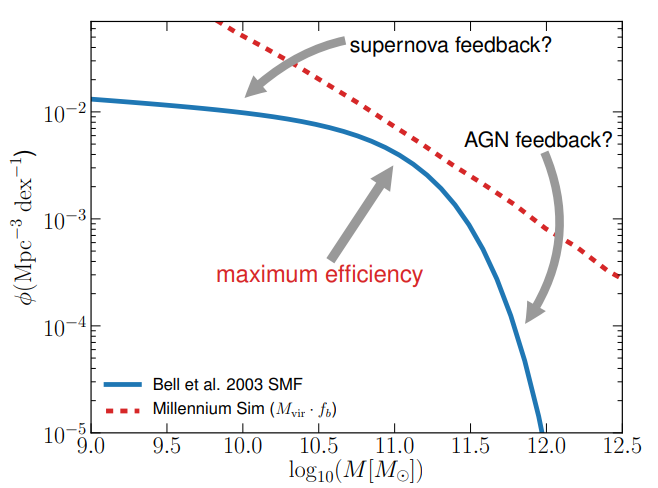
\includegraphics[width=0.58\textwidth]{plots/feedback.png}
	\caption{A comparison between the observed galactic stellar mass function (blue) and the distribution expected from the $\Lambda\mathrm{CDM}$ model for perfectly efficient star formation (red). The former is taken from \citet{bell2003optical}, while the latter is obtained by considering the HMF from the Millennium Simulation \citep{Springel:2005nw} and multiplying it for the universal baryon fraction.
    The different slopes at low and high masses between the two lines indicate that star formation is less efficient in these regions. Taken from Mutch et al. \citep{mutch2013simplest}.
	}
	\label{fig:halo_stellar}
    \end{figure}
  


 Besides impacting the star formation rates in galaxies, the presence of feedback in the form of outflowing gas has dramatic consequences for the nearby CGM/IGM. The Circum-Galactic Medium is conventionally defined as the region between the external limits of the galaxy and the virial radius of its dark matter halo. As gas flows out of the galaxy, it floods into the CGM, affecting its properties such as composition, temperature, density, and radial velocity. The wind interacts hydrodynamically with the pre-existing CGM, and gravitationally with the halo's dark matter. Ultimately, the fate of the outflowing baryons depends on both of these processes: they can either be shocked and slowed down, or they can expand freely into the IGM. In the first scenario, the gravitational pull of the DM halo stops the outflows completely, and baryons eventually fall back into the galaxy, creating a "\textit{galactic fountain}" \citep{oppenheimer2006} that refuels the ISM with the same recycled gas that had left the galaxy in the form of an outflow. In the second one, baryons can leave the galaxy and mix with the primordial gas that does not reside in any collapsed structure. This mixing process alters the composition of the primordial IGM, as its metallicity increases because of the contribution of outflowing gas. Metal enrichment (or pollution) of the IGM/CGM via galactic outflows is considered to be the most promising way to explain why roughly half of the metals in the local universe are located outside galaxies, even though they were formed only inside them \citep{menard2010measuring}.
 
 The evolution of outflows as they expand into the CGM parallels with the presence of inflows due to the accretion of gas on the galaxy. This inflowing gas can either cool down from a hot baryons reservoir in the halo or take the form of cold streams  (section \ref{sec:accretion}). Either way, inflowing gas interacts with the outflowing one in a complex interplay that is very difficult to frame, both observationally and with numerical simulations. The combined presence of outflows, inflows, galactic fountains, and diffuse hot gas shapes the CGM (for a cartoon picture, see figure \ref{fig:cgm_cartoon} in chapter \ref{chap:halos}). Their action is known as the \textit{cosmic baryon cycle}: baryons are ejected out of the galaxy thanks to galactic winds, but at the same time they are recycled inside by cosmic accretion and galactic fountains. Overall, these two competing mechanisms steer the galaxy's evolution, as outflows suppress the formation of stars, while inflows enhance the SFR by providing new cold gas to the ISM. For this reason, the CGM is one of the key regions to focus on in order to gain insights into how galaxies evolved through cosmic times. In this work, we deal with these problems by studying some observations of the CGM of high redshift ($z\sim 4-6$) galaxies, and by connecting the observational evidence to the presence of galactic outflows.  

 


\chapter{Galactic outflow physics} \label{chap:outflows}
\vspace{20pt}




\begin{comment}

MAIN REFS


HECKMANN\&THOMPSON, VEILLEUX ET AL 2020, ZHANG 18,

PHD THESIS GV

MAYBE SOMETHING WITH AGN FEEDBACK?


SUMMARY 


 1. INTRO: IMPORTANCE OF FEEDBACK AND LINKS WITH PREVIOUS CHAPTER
 
 1A. OBSERVATIONAL PROBES?
 
 2. DIFFERENT KIND OF OUTFLOWS: AGN-POWERED AND SF-POWERED
 
 3. DIFFERENT PHYSICAL MECHANISMS

 4. THE CC85 MODEL
 
 5. ROLE OF RADIATIVE COOLING 
 
 6. RADIATION PRESSURE POWERING OUTFLOWS
 
 7.  COSMIC RAYS POWERING OUTFLOWS
 
 8. BRIEF OVERVIEW OF THE AGN ROLE?
 
 9. SUMMARY OF WHAT WE KNOW AND WHAT WE WILL DISCOVER IN THE FUTURE
 
 
USEFUL THINGS TO MENTION
 - CC85 MODEL
 - INTRODUCING RADIATIVE COOLING \& THOMPSON'S WORK
 - 
 
\end{comment}


In 1957, the astrophysicist Eugene Parker suggested for the first time that a constant stream of particles could travel from the Sun's atmosphere to the outer regions of the Solar System due to pure hydrodynamic effects \citep{parker_wind}. This hypothesis challenged the conventional wisdom of that time, as the atmospheres of stars like the Sun were thought to be essentially in hydrostatic equilibrium. Two years later, this so-called \textit{Solar Wind} has been observed for the first time, and since then, we have become more and more aware of the ubiquity of stellar winds and of their impact on the circumstellar environment.


In the same years, "evidence for
an explosion in the center of the galaxy M82" was reported \citep{lynds_m82}: it was the first observation of gas outflowing from a galaxy. M82 has since then become the prototypical starburst galaxy, hosting a well-studied bipolar galactic wind created by SNe activity (figure \ref{fig:m82}). As authors created models for the formation of these winds on galactic scales \citep{chevalier_clegg:1985} -- using principles similar to the ones presented in the theory of stellar winds \citep{stellar_winds_holzer} -- new observations proved the presence of a greater and greater number of outflows in galaxies with different age and properties \citep{osterbrock_1960, burke_1968}. 

Today, we know that outflows are ubiquitous in starburst galaxies in the local universe, and, most importantly, in normal star-forming galaxies at medium and high redshift. As described in chapter \ref{chap:intro}, these winds are believed to play an essential role in shaping up the universe as we know it, being the main source of feedback mechanisms through which galaxies determine their own evolution. 

In this chapter, we focus entirely on the theory of galactic winds, describing their properties and their driving mechanisms. We give a brief overview of the main characteristics of outflows in section \ref{sec:intro_outflows}, exploring their nature and the information we can gain from observations. Then, we look into the theory of Supernovae-driven outflows in section \ref{sec:model_outflows}, focusing in particular on the formation mechanisms of the cold winds that are routinely witnessed in observations. 

Throughout this chapter, we will mainly follow the reviews by Veilleux et al. \citep{Veilleux:2005ia, veilleux2020cool}, Heckman \& Thompson \citep{heckman2017galactic}, Zhang \citep{zhang2018review}, and Rupke \citep{rupke2018review}. 



\begin{figure}
    \centering
    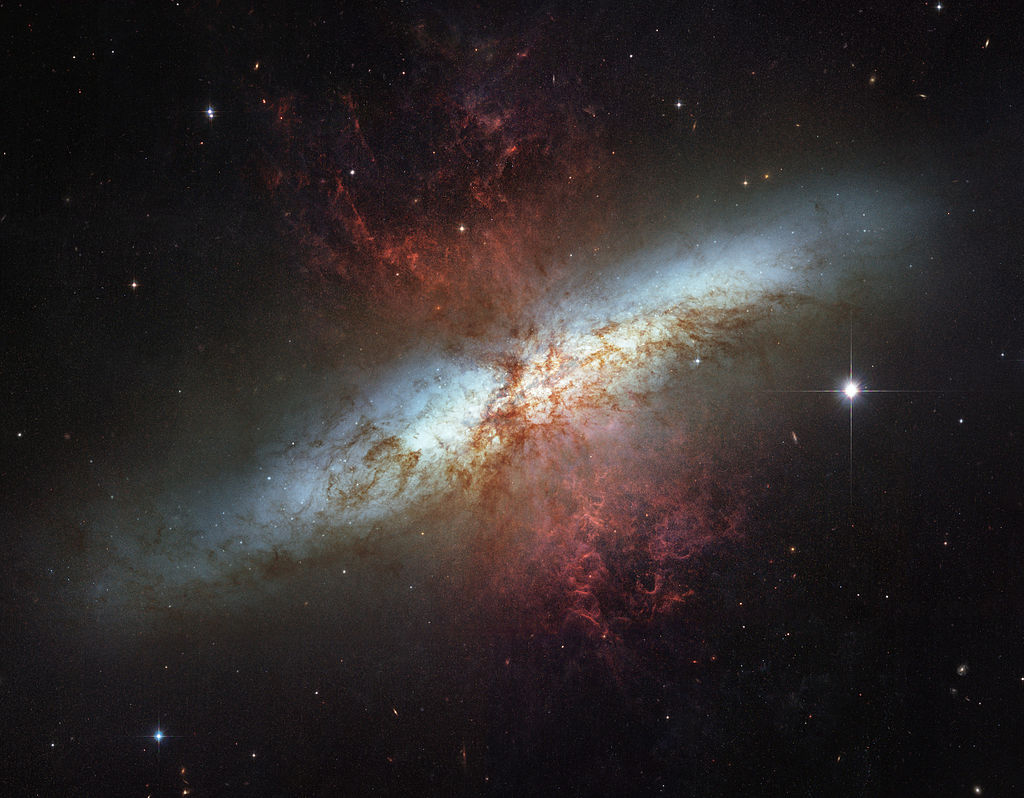
\includegraphics[width=0.58\textwidth]{plots/m82.jpg}
    \caption{Image of M82 taken by the Hubble Space Telescope (HST). The emission coming from the H$\alpha$ line (red), measured with the Subaru telescope, has been superimposed to the original HST image. Figure from the Hubble telescope
    gallery. }
    \label{fig:m82}
\end{figure}


\section{General properties} \label{sec:intro_outflows}


\subsection{Star formation and AGN driven outflows}

As already mentioned in chapter \ref{chap:intro}, outflows are thought to form both during starburst episodes (i.e., intense episodes of star formation) and during active accretion of gas on a SMBH. The former ones are driven by the energy and momentum released by stellar winds and Supernovae, while the latter ones are driven by AGN radiation or jets.

AGN feedback mechanisms are the most powerful and extreme events: for this reason, they are thought to play a relevant role in affecting the properties of even the most massive galaxies in the universe (section \ref{sec:feedback}). In the standard picture, AGN feedback is believed to operate in two different modes: a \textit{radiative} (also known as \textit{quasar}) mode and a \textit{kinetic} (\textit{radio}) mode. 

The \textit{radiative mode} is associated with very high BH accretion rates, and it is able to create powerful winds driving gas out of the galaxies \citep{silk_rees_agn}. It operates on short timescales, as the resulting strong AGN emission and powerful outflows deplete the gas reservoir in the central regions of the galaxies, quenching star formation, and, at the same time, compromising the efficiency of gas accretion on the central SMBH. Strong winds are produced in this mode thanks to the enormous amount of radiation emitted by the central AGN: the pressure associated with this radiation can accelerate a fast wind in the proximity of the SMBH. The wind - which can reach a substantial fraction of the speed of light \citep{kraemer2018physical} - impacts directly on the surrounding medium, generating a shock and thus accelerating the interstellar gas. 

\textit{Energy-driven} winds form when the shocked ISM retains its energy, expanding adiabatically on kpc scales. If the shocked gas can cool efficiently, on the other hand, a \textit{momentum-driven} wind is formed: the gas conserves its momentum but not its energy, and thus the resulting outflow is not as fast and strong as in the former scenario. We will deal with the problem of radiative cooling of the outflowing gas in section \ref{sec:outflows_cooling}. 

The \textit{kinetic mode}, instead, forms in low-luminosity AGN, where gas accretion is not as strong and the resulting radiation is not able to drive fast winds in the galaxy. This mode, however, is extremely important, as it is able to quench star formation by preventing the halo gas to accrete into the galaxy. This \textit{preventative feedback} acts by heating the CGM gas, and thus balancing the radiative cooling rate and inhibiting the ability of the gas to cool and fall into the galaxy (section \ref{sec:infall_and_cooling}). Jets, created by AGN, are thought to be responsible for this heating process thanks to their kinetic energy. This mode has large timescales, as low accretion rates on SMBHs can be sustained over longer periods of time. 

Overall, it is the combined action of radiative and kinetic mode that makes AGN feedback effective in governing the star formation rate in massive galaxies \citep{fabian12}. However, details of these processes are still lacking: despite the increasing number of AGN-powered outflows observed at low and high redshift in the last few years \citep{feruglio2010quasar, maiolino2012evidence, carniani2015ionised,Fiore_2017, cicone2018largely}, the actual mechanisms governing these outflows, as well as their impact on the host galaxies are still difficult to constraint observationally.  

Winds driven by star formation processes are in general slower and less powerful; their velocities range between a few hundred to $1000\,\kms$. For this reason, they are thought to play a major role in low-mass galaxies as well as in high redshift galaxies, where the presence of AGN becomes less common. In other respects, they are similar to the AGN radiative mode winds, but the underlying driving mechanism is different: the combined effect of stellar winds from hot stars and SNe injects into the interstellar regions hot and metal-enriched material, which can become buoyant and leave the galaxy. Note, however, that different driving mechanisms have been proposed, including radiation pressure and cosmic rays \citep[e.g.,][]{recchia_cosmic_rays, zhang_rad_pressure}.

In this work, we will focus entirely on winds driven by star formation activity: in the following sections, when not stated otherwise, we will refer to winds connected with Supernovae and hot stars. This is because our model aims to explain observations of galaxies that do not show any sign of AGN activity (chapter \ref{chap:halos}). However, in section \ref{sec:results}, we will describe how our results hint at the possibility of an obscured AGN contribution in driving outflows in the sample of galaxies considered. 




\subsection{Observational properties} \label{sec:obs_outflows}

One of the main challenges related to outflows studies is to turn observations into quantitative measurements of the basic fundamental properties of outflows. Such measurements are in fact required in order to study outflows' driving mechanisms and physical properties, and to assess how and to which extent outflows affect the central galaxy and its gas reservoir. 

The most basic quantity that is possible to infer from observations is the outflow velocity ($v$). This is because outflows are often revealed by studying absorption/emission spectral lines of galaxies. Therefore, measuring the extent of the broad-wing feature (created by the relative velocity of outflowing gas) in these lines gives a direct estimate of the wind velocity. However, contamination due to the central ISM kinematics and other similar effects can bias this measurement. In order to overcome this obstacle, different prescriptions are possible, e.g., considering only the most extreme part of the broad line component. Even though several conventions can be employed, they are broadly consistent; for this reason, the wind velocity can be considered as the most reliable quantity that can be deduced from observations. 

 
Using velocity measurements, the mass outflow rate $\dot{M}_\mathrm{out}$ can be obtained by making use of a relation based on simple dimensional analysis:
\begin{equation}
        \dot{M}_\mathrm{out} = \frac{M_\mathrm{out}v}{r_\mathrm{out}},
\end{equation}
where $M_\mathrm{out}$ is the total mass of the outflowing gas contained in a radius $r_\mathrm{out}$. In turn, the mass outflow rate can be used to compute other two relevant quantities: the kinetic energy rate ($\dot{E}_{k,\mathrm{out}} = \dot{M}_\mathrm{out}/2v^2$) and the momentum rate ($\dot{P}_\mathrm{out} = \dot{M}_\mathrm{out}v$).

Gas masses and outflow radii are quite difficult to obtain. Size measurements are possible only for spatially resolved observations. Otherwise, typical outflow sizes must be assumed, introducing a relevant source of error in the rate computation. Even when spatially-resolved observations are available, different criteria can be used to compute outflow sizes. Furthermore, the precise meaning of $r_\mathrm{out}$ inevitably depends on the particular morphology of the outflow. As for gas masses, they can be inferred by noting that the luminosity of the outflow is proportional to the volume integral of $n^2$, and hence to the product of $M_\mathrm{out}n_\mathrm{out}$. Gas densities can be measured by warm gas lines, but they depend on the ionization state and the element abundances in the gas. Therefore, measurements of outflow rates are often subject to many sources of uncertainty, and their values can be estimated only on a very coarse level.

Mass outflow rates are often parametrized also in terms of the mass loading factor $\eta = \dot{M}_\mathrm{out}/\mathrm{SFR}$. Assuming mass conservation in the outflow, this quantity can also be described as the ratio between the rate of ISM gas mass that is loaded in the outflow and the star formation rate. This quantity plays a relevant role in the context of feedback mechanisms and star formation quenching, as high values of $\eta$ imply that fraction of ISM gas that is expelled from the galaxy is higher than the one that contributes to forming stars. This can ultimately lead the galaxy to run out of gas, quenching any subsequent SF activity (section \ref{sec:feedback}). The mass loading factor will play a key role in subsequent chapters.

\subsection{The multiphase nature of galactic winds} \label{sec:multiphase}



The picture emerging from outflows' observations is complex and difficult to interpret. In particular, it has been thoroughly proved by multi-wavelength surveys that outflowing gas hosts a wide variety of thermodynamical conditions: hot and highly ionized gas is often mixed with cold, neutral, or even molecular gas. This fact represents one of the greatest theoretical and observational challenges linked with the physics of outflows, as it poses a range of questions whose answers are still far from clear:
\begin{itemize}
    \item Which is the relative contribution of the different phases to the energy, mass, and metals budget of the outflow?
    \item Provided that the driving mechanism for SN-driven winds is effective only for hot gas, how is the colder gas formed in the outflow? 
    \item Do different phases have different physical properties and live on different scales?
    \item How do different phases affect the host galaxy via feedback effects? 
\end{itemize} 
Furthermore, observations of outflows are much more difficult in light of their complex nature. Since winds are studied using either emission or absorption spectral lines, individual observations typically give information only on a specific phase, and not on the properties of outflows as a whole. This often hinders a precise assessment of the outflows' role in driving galaxy evolution (see section \ref{sec:feedback}). 


Conventionally, five different phases can be identified, based on the temperature of the gas (or, equivalently, on its ionization state, as the ionization of gas depends primarily on its temperature): a very hot phase ($T\sim 10^8\,\mathrm{K}$), a hot and highly ionized phase ($T\sim 10^{6-7}\,\mathrm{K}$), a warm and ionized phase ($T\sim 10^{4-5}\,\mathrm{K}$), a cool and neutral atomic phase ($T\sim 10^3\,\mathrm{K}$), and a cold and molecular/dusty phase ($T\sim 10-100\,\mathrm{K}$). Each phase can be traced by a different set of species, given that the presence of those species depends on the temperature of the gas. For example, very hot gas will emit in the X-ray, and thus X-ray emission and absorption features can be used to constraint the properties of the gas hot phase \citep{Strickland:2000jg, strickland2009supernova}. In a similar way, ionized species such as \OIII are tracers for the warm phase at $10^4\,\mathrm{K}$, while species such as \CIIion, \HI, \HH, CO trace the atomic neutral and molecular phases. 

Using these tracers, observations tend to agree on the fact that hot outflows are fast ($v\approx 1000\,\kms$) and dominate the kinetic energy budget of the outflowing material. Cold/warm neutral outflows, on the other hand, are found to dominate the total mass outflow rate, and they are often slower, with velocities in the range $v\approx 100-500\,\kms$ \citep[e.g.,][]{rupke2013multiphase}.


\section{Models for star formation driven outflows} \label{sec:model_outflows}

In this section, we review the theory of galactic outflows driven by star formation, by looking at the most important models that have been proposed to explain the formation and evolution of galactic-scale winds. A satisfactory theoretical explanation for the origin of these outflows cannot neglect the observational properties that outflows present at low and high redshifts. 

As described in the last section, the most striking feature of outflows is the presence of many different phases, ranging from the very hot gas to the cold molecular one. The key question is then how these phases are formed within the outflow, and how they evolve over different spatial and time scales. We start by considering the classical model for hot outflowing gas, first proposed by Chevalier \& Clegg in 1985 \citep{chevalier_clegg:1985} (hereafter, CC85). Then, we focus on the warm and cool phases by analyzing gas radiative cooling and the acceleration of the cool gas by the outflowing wind.  



\subsection{CC85 model} \label{sec:cc85_model}

The CC85 model describes a hot and steady wind that drives gas out from the center of the galaxy. The wind is created by the energy and mass released by overlapping Supernovae events. Despite the fact that describing the physical processes leading to the formation of winds from SNe is extremely complex, simple analytical estimates can be applied on galactic scales, where the properties of single events are averaged. In particular, a constant rate of energy and mass injection in the gas is assumed inside the galaxy, modeled as a sphere of radius $R$. 

With these assumptions, the configuration is time-steady and spherically symmetric. In the region inside the sphere of radius $R$, mass and energy are not conserved: we call the source terms $\dot{M}$ and $\dot{E}$ respectively. Outside the spherical region, instead, the gas is assumed to expand adiabatically, conserving both mass and energy. This is a key assumption, as it means that any radiative loss is neglected in the outflow: we will later revise this hypothesis when dealing with cool gas formation. Thermal conductivity and viscosity are neglected as well. Moreover, gravitational effects are considered to be small, since, as we will prove in a moment, the velocity at the edge of the galaxy is much greater than the escape velocity of the gas. 

With these conditions, we can write the two equations for hydrodynamics (mass conservation and Euler equation), closing the system with the energy conservation equation:
\begin{subequations}
\begin{align}
    &\pder{\rho}{t} +\mathbf{\nabla} \cdot (\rho \mathbf{v})=q\\
    &\pder{\mathbf{v}}{t} + (\mathbf{v}\cdot \mathbf{\nabla})\mathbf{v} = - \frac{1}{\rho}\mathbf{\nabla} \cdot P - \mathbf{v}q\\
    &\pder{}{t}\bigg(u+\rho\frac{v^2}{2}\bigg)+\mathbf{\nabla}\cdot\bigg(\mathbf{v}\bigg(h+\rho \frac{v^2}{2}\bigg)\bigg)=Q
\end{align}
\end{subequations}
In these expressions, $\rho, v, p$ are the gas density, velocity, and pressure respectively; $u$ is the internal energy density per unit volume, while $h$ is the enthalpy per unit volume ($h=u+P$). Using the definition of the internal energy ($u=(\gamma -1)^{-1}nkT$), as well as gas equation of state (eq. \ref{eq:state_equation}), we can rewrite the enthalpy as: 
\begin{align}
   h = \frac{\gamma}{\gamma -1} \,P,
\end{align}
where $\gamma = 5/3$ is the adiabatic index.

The mass input rate $q$ and energy input rate $Q$ per unit volume - assumed to be constant in space and time - take the form:
\begin{equation}
\begin{cases} q=\frac{3\dot{M}}{4\pi R^3}\,, \,\,\,r\le R\\ q=0\,, \,\,\,r> R \end{cases}
\qquad \begin{cases} Q=\frac{3\dot{E}}{4\pi R^3}\,, \,\,\,r\le R\\ Q=0\,, \,\,\,r> R \end{cases}
\end{equation}

With these definitions, we can search for a steady-state solutions by dropping the partial time derivative terms. Using spherical coordinates, we get:
\begin{subequations} \label{eq:eul_cc85}
\begin{align}
&\frac{1}{r^2}\der{}{r}(r^2v\rho)=q  \label{eq:eul1_cc85}\\
&\rho v\der{v}{r}= -\der{p}{r} -vq \label{eq:eul2_cc85}\\
&\frac{1}{r^2}\der{}{r}\bigg[r^2\rho v\bigg( \frac{v^2}{2}+\frac{\gamma}{\gamma -1}\frac{p}{\rho}\bigg)\bigg]=Q, \label{eq:eul3_cc85}
\end{align}
\end{subequations}

Imposing appropriate boundary conditions for the system $v(0)=0$, $\rho(r\rightarrow+\infty)=T(r\rightarrow+\infty)=0$, we can solve the equations in the two regions. By requesting a smooth transition between the two solutions, we find that this model describes an outflow transitioning from a sub-sonic regime in the inner region to a super-sonic adiabatic expansion in the outer one. The general solution can thus be conveniently expressed in terms of the Mach number $\mathcal{M} = v /c_s$, which is defined by considering the sound speed of the gas:
 \begin{align}
   c_s^2 =\gamma\,\frac{P}{\rho} = \gamma\, \frac{k_B}{\mu m_p} T \label{eq:sound_speed}
 \end{align}
 The solutions in the two regions, then, reads: 
\begin{align}
&\bigg(\frac{3 \gamma + 1/\mathcal{M}^2}{1+3 \gamma}\bigg)^{-(3\gamma+1)/(5 \gamma+1)}\bigg(\frac{\gamma-1+2/\mathcal{M}^2}{1+\gamma}\bigg)^{(\gamma+1)/(2(5\gamma+1))} = \frac{r}{R} \label{eq:solinn}\\
&\mathcal{M}^{2/(\gamma-1)}\bigg(\frac{\gamma-1+2/\mathcal{M}^2}{1+\gamma}\bigg)^{(\gamma+1)/(2(\gamma-1))} = \bigg(\frac{r}{R}\bigg)^2 \label{eq:solout}\,,
\end{align}
where eq. \ref{eq:solinn} (eq. \ref{eq:solout}) applies to $r<R$ ($r>R$). To grasp the properties of these solutions, it is useful to introduce dimensionless variables ($r_*$, $v_*$, $\rho_*$, and $P_*$) using the input quantities $R$, $\dot{M}$, $\dot{E}$, as a unit radius, mass rate, and energy rate respectively:
\begin{subequations} \label{eq:dimensionless_cc85}
\begin{align}
    &r = r_* \,R\\
    &v = v_*\,\dot{E}^{1/2}\,\dot{M}^{-1/2}\\
    &\rho = \rho_*\,\dot{E}^{-1/2}\,\dot{M}^{3/2}\,R^{-2}\\
    &P = P_*\,\dot{E}^{1/2}\,\dot{M}^{1/2}\,R^{-2}
\end{align}
\end{subequations}
Figure \ref{fig:cc85} shows the profiles for the dimensionless parameters $v_*$, $\rho_*$, and $P_*$, as a function of the dimensionless radius $r_*$. As already noted, the solution represents an outflow undergoing a sonic transition (i.e., $\mathcal{M} = 1$) at $r_* = 1$: for smaller radii, the velocity increases monotonically, while density and pressure slowly decrease; near the sonic point, profiles steepen as they present a divergence in the first derivative at $r_*=1$. Then, the flow transitions to a super-sonic adiabatic expansion, with the velocity reaching an asymptotic value, and the pressure and density decreasing with a power-law scaling. Numerical estimates of these scalings can be easily determined considering eqs. \ref{eq:eul_cc85}: in the outer region $Q=q=0$, hence mass conservation yields $\rho v r^2 = \mathrm{const.}$, while energy conservation can be recast in the form of a Bernoulli integral conservation: 
\begin{align}
 B = \frac{v^2}{2} + \frac{\gamma}{\gamma -1}\,\frac{P}{\rho} = \mathrm{const.} = \frac{\dot{E}}{\dot{M}}, \label{eq:bernoulli}
\end{align}
where the last equality can be inferred simply noting that the Bernoulli integral represents the total energy per unit mass of the fluid. At infinity, the second term in eq. \ref{eq:bernoulli} vanishes: we then find $v_\infty = \sqrt{2}\,\dot{E}^{1/2}\,\dot{M}^{-1/2}$ (i.e., $v_{*,\infty} = \sqrt{2}$). Knowing that the velocity in asymptotically constant, we easily infer that density scales as $\rho\sim r^{-2}$ to conserve the mass; hence, pressure and temperature scales as $r^{-2\gamma}$ and $r^{-2(\gamma-1)}$, as the adiabatic equation holds ($P\rho^{-\gamma}=\mathrm{const.}$). 

Numerical values at the sonic point ($v(R)$, $\rho(R)$, $P(R)$) can be determined simply considering eq. \ref{eq:bernoulli}, setting $v=c_s$ ($\mathcal{M}=1$), and integrating eq. \ref{eq:eul1_cc85} in the inner zone:
\begin{subequations}
\begin{align}
    &v_*(R) = \left(\frac{1}{2}+\frac{1}{\gamma-1}\right)^{-1/2}\label{eq:bound_cc85_1}\\
    &\rho_*(R) = \frac{1}{4\pi v_*}\\
    &P_*(R) = \frac{v_*}{4\pi \gamma}\label{eq:bound_cc85_3}
\end{align}
\end{subequations}

The physical relevance of the CC85 model can be appreciated by setting some reasonable input values for the mass and energy inputs. As already described in section \ref{sec:feedback}, the energy input from SNe can be parametrized by introducing the energy released by a single SN ($E_{0,\mathrm{SN}}$) and the frequency of SNe per unit mass $\nu_\mathrm{SN}$. We choose $E_{0,\mathrm{SN}} = 10^{51}\,\mathrm{erg}$ \citep{ostriker_supernovae} and $\nu_\mathrm{SN} = 10^{-2}\,\msun^{-1}$ (this holds true for a Salpeter IMF \citep{leitherer1999}, see also sec. \ref{sec:star_formation}). With these parameters, both the energy and the mass input rates can be expressed as a linear function of the star formation rate. We introduce two efficiency factors, the thermalization efficiency $\alpha$ and the mass loading factor $\eta$ (seec. \ref{sec:obs_outflows}), to parametrize the coupling between SNe ejecta and the outflowing gas:
\begin{subequations}
\begin{align}
    &\dot{E}=\alpha  E_{0,\mathrm{SN}} \nu_\mathrm{SN} \,\mathrm{SFR}\\
    & \dot{M}=\eta \, \mathrm{SFR}
\end{align}
\end{subequations}

With these choices for the input parameters, the terminal velocity of the outflow is independent of the SFR: $v_\infty \approx 10^3\,\mathrm{km}\,\mathrm{s}^{-1} \,( \alpha / \eta )^{1/2}$. For values of $\alpha$ and $\eta$ close to unity, this velocity is much greater than the circular velocity of galaxies, hence gravity does not play a relevant role in the model. When examining radiative cooling outflows, this hypothesis will not hold true, as the outflows slow down because of thermal losses and they are affected by the halo gravitational potential (section \ref{sec:cooling_gravity}). 

Other useful quantities are the temperature and density at the critical point $r=R$:
\begin{subequations}
\begin{align}
    & T(R) \approx 2\times10^7\,\left(\frac{\alpha}{\eta}\right)\\
    & n(R) \approx 1\times10^{-2}\,\mathrm{cm}^{-3}\,\left(\frac{\mathrm{SFR}}{1\,\msun\,\mathrm{yr}^{-1}}\right) \left(\frac{R}{1\,\mathrm{kpc}}\right)^{-2}\,\left(\frac{\eta^{3/2}}{\alpha^{1/2}}\right)
\end{align}
\end{subequations}
These quantities will play an important role in subsequent discussion (chapter \ref{chap:model}). 

Overall, the CC85 model describes an outflow with high temperature, relatively low density, and high terminal velocities. These quantities are compatible with X-rays observations of the hot phases of outflows in local starburst galaxies: estimates of the two efficiency parameters from these observations hold $\alpha=0.3-1$, $\eta=0.2-0.6$  \citep[e.g.,][]{strickland2009supernova, zhang2014hot}. 

This model has thus become the standard way to approach the problem of adiabatic hot flows. Several works have confirmed the main results of the model in numerical hydrodynamical simulations, both in idealized setups \citep{Strickland:2000jg} and in realistic 3d cases \citep{cooper2009starburst, schneider2018production}. Variations on the model have also been proposed: for instance, Bustard et al. \citep{bustard2016versatile} have considered a more realistic non-uniform profile for the input region, also including the contribution of the galaxy gravitational potential. They have shown that in this less idealized scenario the non-physical divergence in the first derivative of thermodynamical variables disappears, and the sonic point does not coincide with the edge of the galaxy for a general mass input profile. However, quantitative conclusions for the CC85 model hold true even in this case: the only approximation that ceases to be valid for some values of the input parameters is that the outflow evolves adiabatically. In the next section, we will focus on this approximation, describing how a hot flow is able to cool down thanks to radiative losses, and how this impacts the subsequent evolution of the wind.  




\begin{figure}
    \centering
    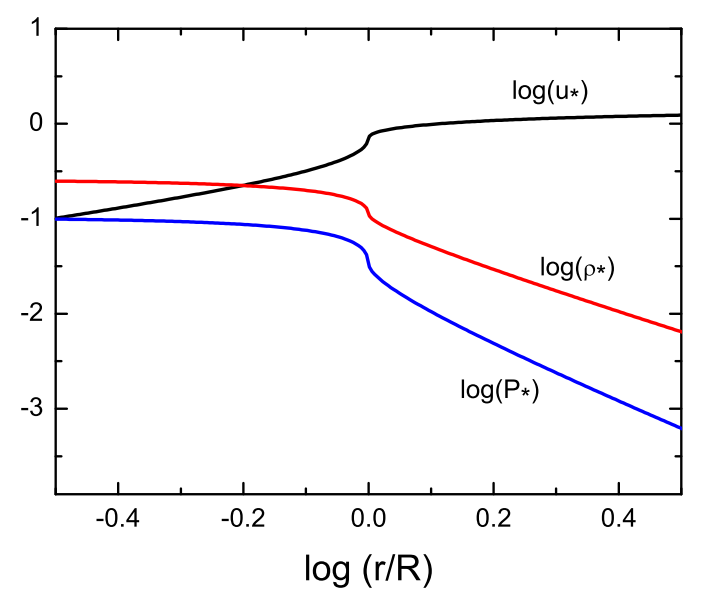
\includegraphics[width=0.5\textwidth]{plots/cc85.PNG}
    \caption{Radial solutions for the CC85 model \citep{chevalier_clegg:1985}. The black, red, and blue lines show the profiles for the dimensionless parameters $u_*$, $\rho_*$, and $P_*$ (eqs. \ref{eq:dimensionless_cc85}) respectively, as a function of the dimensionless radius $r_*=r/R$. Figure taken from \citet{zhang2018review}.
    }
    \label{fig:cc85} 
\end{figure}




\subsection{Cold flows and related problems}\label{sec:outflows_cooling}


While the physics underlying the formation and evolution of hot flows is well established, the presence of cold gas outflowing at high speed (hundreds of $\kms$) from galaxies has represented a formidable theoretical problem in the last two decades. The fundamental question that needs to be answered is how to accelerate cool atomic and warm ionized gas to these velocities, as the cold gas is not buoyant and thus is not able to form a wind on its own. Two mechanisms have gained momentum in the literature: in the first one, the ram pressure of hot outflowing gas accelerates the cold ISM, creating a cool phase in the outflow; in the second one, hot gas cools by emitting radiation and thus forming a warm (and possibly cool) uniform phase. We will review both these explanations in the next paragraphs, as they will be relevant in the development of our model in the following chapters. 


\subsubsection{Acceleration of warm/cool clouds in hot winds}

According to the first mechanism, cold gas in outflows comes from ISM material that is accelerated and entrained in the hot wind. The factor that is responsible for accelerating the gas is generally identified in the ram pressure of the hot flow (however, other driving mechanisms are possible, e.g., radiation pressure on dust). In fact, since the hot outflow is highly supersonic in the external region (eq. \ref{eq:solout}), its ram pressure is much greater than its thermal pressure, and thus it can transfer momentum to the cold material in the ISM driving it to velocities as high as thousands of $\kms$. 

A good estimate for this momentum exchange rate can be obtained by considering a simple model of a uniform spherical cold cloud at rest in a flow of hot gas with velocity $v_\mathrm{hot}$ and density $\rho_\mathrm{hot}$. Defining the radius of the cloud $R_c$ and its density $\rho_c$, one can equate the force acting on the cloud because of the flow's ram pressure $\rho_\mathrm{hot}\,v_\mathrm{hot}^2 \,\pi\,R_c^2$ to the rate of change of the cloud momentum. The acceleration timescale $t_\mathrm{acc}$ in which the cloud's velocity reaches $v_\mathrm{hot}$ is then:
\begin{align}
       \tau_\mathrm{acc} = \frac{4R_c}{3v_\mathrm{hot}}\,\frac{\rho_c}{\rho_\mathrm{hot}}
\end{align}
We can get a rough estimate for this timescale considering the typical radius for a cloud $R_c \sim 100\,\mathrm{pc}$, and setting the temperature of the cloud to $T_c \sim 10^4\,\mathrm{K}$ (i.e., the equilibrium value at which photoheating balances radiative cooling; see section \ref{sec:cooling_function}). At this temperature, the Jeans scale of the cloud is much greater than $R_c$ for a wide range of densities. Hence, the cloud must be pressure-confined by the hot medium: for this reason, the density ratio $\rho_c/\rho_\mathrm{hot}$ is equal to the inverse of the temperature ratio $T_\mathrm{hot}/T_c$. According to the CC85 model, the hot medium has a temperature of $T_\mathrm{hot}\sim 10^7\,\mathrm{K}$ near the boundary region $r=R$; we thus get $\rho_c / \rho_\mathrm{hot} \sim 10^3$. Further setting $v_\mathrm{hot} \approx 10^3 \,\kms$ in adherence to CC85, we find that the acceleration time scales as $\tau_\mathrm{acc}\approx 100\,\mathrm{Myr}\, (R_c/100\,\mathrm{pc})$. In principle, since this timescale is smaller than the Hubble time, this acceleration mechanism could be responsible for creating the cold phase in galactic winds.

However, this estimate does not take account of the disruptive effect the hot flow has on the cloud. In fact, as the supersonic wind encounters the cloud at rest, it drives a shock into the overdense gas. The velocity with which this shock travels inside the cloud, $v_s$, can be determined by using the following argument (for more details, see \citep{klein_1994, scannapieco2015launching}): if the shock is highly supersonic, then the pressures on the two sides of the shock are approximately equal. The post-shock pressure is $\rho_\mathrm{hot}\,v_\mathrm{hot}^2$, while the pressure behind the shock (inside the cloud) is $\rho_c \,v_s^2$. Equating these two quantities, we get an expression for the velocity of the shock:
\begin{align}
    v_s = v_\mathrm{hot}\,\left(\frac{\rho_\mathrm{hot}}{\rho_c}\right)^{1/2}
\end{align}
Thus, we can introduce another important timescale, the \textit{cloud-crushing time} $t_{cc}$, by considering the time it takes the shock to travel through the cloud, heating and disrupting it in the process. Using the expression for $v_s$, we find:
\begin{align}
    t_{cc} \sim \frac{R_c}{v_s} \sim \frac{R_c}{v_\mathrm{hot}}\,\left(\frac{\rho_c}{\rho_\mathrm{hot}}\right)^{1/2}
\end{align}
As the cloud is heated and shredded by the shock, we expect that its complete destruction happens in a few cloud-crushing times: this was proven using hydrodynamical simulations as early as 1994 by Klein et al. \citep{klein_1994}. In figure \ref{fig:cloud_crushing}, we show a more recent simulation by Schneider \& Robertson \citep{schneider2017hydrodynamical} of a $10\,\mathrm{pc}$ cloud being disrupted by the hot flowing gas. 

If we compare the cloud-crushing time with the acceleration time, we note that, as long as $\rho_c\gg\rho_\mathrm{hot}$, $\tau_{cc}\ll\tau_\mathrm{acc}$. This poses a serious issue to the theory of accelerating clouds, as it predicts that clouds are always disrupted and incorporated into the hot wind before they can be accelerated to the velocities usually measured by observations. In order to solve this problem, several works have focused on taking into account different physical processes that are usually neglected in the basic picture: in particular, the presence of radiative cooling, thermal conduction, and magnetic fields have been proven to prolong the clouds lifetime. 

Radiative cooling allows the cold gas to survive longer as it can quickly radiate away the thermal energy gained by the interaction with the shock wave. If cooling is efficient, then the cloud can survive the shock, but it is nevertheless destroyed in a time proportional to $\tau_{cc}$ by hydrodynamical instabilities. Simulations show that this destruction timescale is dominated by shear instabilities and scales as $t_{cc}\,\sqrt{1+\mathcal{M}_\mathrm{hot}}$ \citep{scannapieco2015launching}. 

Thermal conduction driven by free streaming electrons in the hot flow also plays a relevant role: as shown by a number of works \citep[e.g.,][]{bruggen2016launching}, the outer layers of the cloud evaporates because of conduction; the core regions, instead, are stretched into dense and cold filaments, in a process that has the overall effect of stabilizing the cloud against hydrodynamical instabilities. These cold filaments, however, have a smaller cross-section with the hot flow, and therefore they are accelerated less efficiently by the wind. Finally, magnetic fields have been shown to significantly increase both the lifetime of the cloud and the drag force accelerating it \citep{mccourt2015magnetized}.

Although the combined effect of these processes could in principle extend the lifespan of cold gas and account for the cold phase observed in multiphase galactic winds, it remains unclear whether this picture is realistic enough, as simulations are efficient only in describing very idealized setups. Overall, the problem of how to accelerate cold ISM material driving it to a substantial fraction of the hot phase's velocity remains yet to be solved. For this reason, a different explanation for the cold phase of galactic winds has been proposed: in this alternative scenario, the cold phase precipitates directly from the hot flow because of radiative cooling. We examine the physics involved in this mechanism in the next paragraph.




\begin{figure}
    \centering
    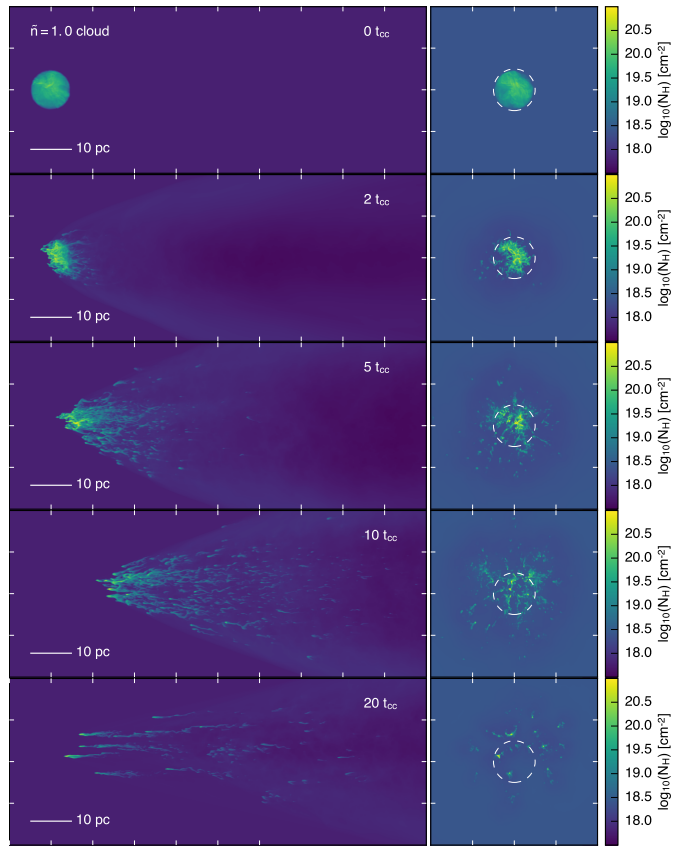
\includegraphics[width=1.0\textwidth]{plots/cloud_crushing.PNG}
    \caption{Time series evolution of a turbulent cloud entrained in a hot flow. Plots on the left show the surface density projected along the y-axis, with the wind entering the box from the left, while the right column shows the surface density projected in the direction of the wind velocity. Snapshots are shown at $t = 0, 2, 5, 10,$ and $20\,t_{cc}$. Cooling is included in the simulation: this allows the cloud to survive for around $10\,t_{cc}$ before being disrupted by the hydrodynamical instabilities. Taken from Schneider \& Robertson \citep{schneider2017hydrodynamical}.
    }
    \label{fig:cloud_crushing}
\end{figure}


\subsubsection{Radiatively cooling outflows} \label{sec:thompson_model}


In 1995, Wang \citep{Wang:1995} was the first one to point out that gas in the CC85 model can radiate a non-negligible amount of energy, and thus the wind can significantly depart from a simple adiabatic evolution in the region outside of the galaxy. This possibility has been widely studied by a number of different works, both in the context of galaxies \citep{McCourt:2015, sarkar:2015, Thompson16, Scannapieco:2017, Schneider:2018, Gronke&Oh:2020, fielding2021} and super-star clusters (SSC) \citep{Silich:2004, tenorio2003supergalactic, tenorio2007hydrodynamics, gray2019catastrophic, danehkar_2021}.


As pointed out by Thompson et al. \citep{Thompson16}, it can be proven that CC85-like highly mass-loaded winds inevitably cool on large scales. The reason for this can be inferred by comparing the cooling timescale $\tau_\Lambda$ (eq. \ref{eq:tcool}) with the \textit{advection time} $\tau_\mathrm{adv} = r / v(r)$ (i.e., the time it takes a fluid element to travel a unit distance). The discussion here echoes the study of the accretion mechanisms of the halo gas on the galaxy (section \ref{sec:accretion}): if the cooling timescale is longer than the advection time, then the evolution of the wind can be considered adiabatic, because the fluid element is brought to large distances from the galaxy before it is able to radiate away its energy. As the cooling timescale becomes shorter than the advection time, the evolution can depart significantly from the adiabatic one: cooling becomes suddenly very efficient, and the gas temperature drops abruptly in a process known as \textit{catastrophic cooling}. 
%We will describe this process in greater detail in chapter \ref{chap:model}, as it constitutes the core of the model we develop in this work. 

In order to study the conditions for which radiative cooling starts to become efficient, we have to look at the temperature dependence of the cooling function of the gas $\Lambda^\mathrm{(cool)}(T)$: this quantity is defined as $\Lambda^\mathrm{(cool)}(T) = \dot{\varepsilon}/n^2$, where $\dot{\varepsilon}$ is the rate of radiative losses per unit volume.  Note that we are focusing only on the temperature dependence of $\Lambda^\mathrm{(cool)}$ because the cooling function is independent of the gas density in the low density limit (section \ref{sec:gas_cooling_heating}); furthermore, we are neglecting further dependences on the metallicity, on the radiation fields acting on the gas, etc., because in this context we are only interested in very crude estimates. If the temperature is greater than about $10^7\,\mathrm{K}$, the processes that dominate emission are free-free collisions (\textit{bremsstrahlung}): these processes have a temperature dependence that scales as $\dot{\varepsilon}_{ff}\sim T^{1/2}$. Therefore, the cooling timescale reads (see also eq. \ref{eq:tcool}):
\begin{align}
    \tau_\Lambda = \frac{1}{\gamma - 1}\frac{\mu m_p k_B T}{\rho(r)\Lambda^\mathrm{(cool)}(T)} \sim \frac{T^{1/2}}{\rho}
\end{align}
We can express the radial dependence of these variables by supposing that the flow starts adiabatic, and using the scalings of a pure adiabatic expansion as dictated by the CC85 model in the limit of great galactocentric distances (i.e., $r\gg R$): we take the velocity as a constant, while the density decreases as $r^{-2}$ and the temperature as $r^{-4/3}$ (again, we consider $\gamma = 5/3$). Hence, the cooling timescale depends on the radius as $\tau_\Lambda\sim r^{4/3}$. Since $\tau_\mathrm{adv} = r/v \sim r$, the ratio between the cooling and the advection times slowly grows with radius: $\tau_\Lambda/\tau_\mathrm{adv}\sim r^{1/3}$. Therefore, if the flow starts adiabatic and the temperature does not drop under $10^7\,\mathrm{K}$, radiative losses can always be neglected and the entire evolution follows the CC85 model.

Things change when we consider lower temperatures: in the range $10^5\,\mathrm{K}\,\lesssim T\lesssim\, 10^7\,\mathrm{K}$, atomic line emission starts to dominate the cooling function. The temperature dependence in this range can be roughly approximated by a power-law of the form \citep{mac_low_cooling} (valid for solar metallicity):
\begin{align}
    \Lambda^\mathrm{(cool)}(T) = 3\times10^{-23}\,\left(\frac{T}{10^7}\right)^{-0.7}\,\mathrm{erg}\,\mathrm{cm}^3\,\mathrm{s}^{-1}
\end{align}
Thus, in this regime, the cooling time scales as $\tau_\Lambda\sim r^{-4/15}$ and the ratio $\tau_\Lambda / \tau_\mathrm{adv}$ is a steep decreasing function of radius ($\tau_\Lambda / \tau_\mathrm{adv} \sim r^{-19/15}$). For this reason, even if the flow starts adiabatic, there exists a radius $r_\mathrm{cool}$ for which the cooling time gets lower than the advection time. Outward of $r_\mathrm{cool}$, radiative losses are important and the wind rapidly cools down to lower temperature, significantly departing from the adiabatic evolution as the flow slows down and the density tends to increase. 

We can study the importance of these cooling effects by computing the radius $r_\mathrm{cool}$ and comparing it with the size of the galaxy $R$. Again, we work in the asymptotic regime for which $r\gg R$: taking this limit in the solution for the CC85 model (eq. \ref{eq:solout}), we infer the values of $v_\infty$, $T_\infty(r)$, and $\rho_\infty(r)$. Given these quantities, the resulting timescales are: 
\begin{subequations}
\begin{align}
    & \tau_\Lambda \approx 3\times10^6\,\mathrm{yr}\,\left(\frac{\alpha^{2.20}}{\eta^{3.20}}\right)\,\left(\frac{r}{10\,\mathrm{kpc}}\right)^{-0.27}\,\left(\frac{R}{0.3\,\mathrm{kpc}}\right)^{2.27}\,\left(\frac{\mathrm{SFR}}{10\,\msun\mathrm{yr}^{-1}}\right)^{-1}\,\mu \\
    & \tau_\mathrm{adv} \approx 10^7\,\mathrm{yr}\,\left(\frac{\eta}{\alpha}\right)^{0.5}\,\left(\frac{r}{10\,\mathrm{kpc}}\right)
\end{align}
\end{subequations}
From these scalings, we can infer that the cooling radius has a very strong dependence both on $\alpha$ and on $\eta$. In particular, it critically depends on the mass loading factor $\eta$, whose importance will become clear in section \ref{sec:outflow_model}.
\begin{align}
    r_\mathrm{cool} \approx 4\,\mathrm{kpc}\,\frac{\alpha^{2.13}}{\eta^{2.92}}\,\mu^{0.79}\,\left(\frac{R}{0.3\,\mathrm{kpc}}\right)^{1.79}\,\left(\frac{\mathrm{SFR}}{10\,\msun\mathrm{yr}^{-1}}\right)^{-0.79} \label{eq:rcool}
\end{align}
Note that this discussion is valid for a gas temperature in the range $10^5-10^7\,\mathrm{K}$. According to the CC85 model (for $\alpha$ and $\eta$ close to unity), the gas temperature starts higher than $10^7\,\mathrm{K}$ and evolves adiabatically scaling as $r^{-4/3}$. For this reason, our estimate of $r_\mathrm{cool}$ is meant to be only a rough approximation, as it neglects the presence of an internal region where cooling via bremsstrahlung is inefficient. More importantly, our argument does not take into account the possibility that the gas stays adiabatic until the temperature gets lower than $10^5\,\mathrm{K}$. If this happens, then radiative cooling becomes inefficient again (because the cooling function drops at $T\sim10^4-10^5\,\mathrm{K}$, sec. \ref{sec:cooling_function}) and the evolution just proceeds according to the CC85 model: in this case, our estimate of $r_\mathrm{cool}$ does not contain any physical meaning. We can restate this reasoning by providing a minimum value of $\eta$ for which $r_\mathrm{cool}$ falls into the region of the CC85 profile where the temperature is greater than the $10^5\,\mathrm{K}$ threshold. A simple calculation gives:
\begin{align}
    \eta_\mathrm{min} \approx 0.64\,\alpha^{0.636}\,\left(\frac{R}{0.3\,\mathrm{kpc}}\right)^{0.364}\,\left(\frac{\mathrm{SFR}}{10\,\msun\mathrm{yr}^{-1}}\right)^{-0.364}
\end{align}
For $\eta \lesssim \eta_\mathrm{min}$, the wind is adiabatic until arbitrarily large radii, since $\tau_\Lambda/\tau_\mathrm{adv}$ stays always above one. As $\eta$ increases, cooling starts to become efficient, and $r_\mathrm{cool}$ becomes smaller and smaller until it becomes comparable to $R$. For these high values of the mass loading factor, our approximation $r\gg R$ fails, and thus we have to compute the cooling radius using the full CC85 solutions for the $\rho(r)$ and $T(r)$ profiles. We can consider the limit for which $r_\mathrm{cool} = R$; in this case, the corresponding value of the mass loading factor $\eta_\mathrm{crit}$ is:
\begin{align}
    \eta_\mathrm{crit} \approx 1.35\,\alpha^{0.730}\,\left(\frac{R}{0.3\,\mathrm{kpc}}\right)^{0.270}\,\left(\frac{\mathrm{SFR}}{10\,\msun\mathrm{yr}^{-1}}\right)^{-0.270} \label{eq:eta_crit}
\end{align}
As $\eta$ approaches $\eta_\mathrm{crit}$, the cooling radius gets closer and closer to the boundary region $r=R$. This suggests considering the effects of radiative cooling also for $r<R$ (i.e., inside the galaxy), where mass and energy are deposited according to the CC85 model. A number of different works have dealt with this problem, showing that for $\eta \lesssim \eta_\mathrm{crit}$ radiative cooling is efficient in the central region of the galaxy, and that rapidly cooling gas does not take part in the outflow, effectively lowering the mass loading factor \citep[for details, see][]{tenorio2007hydrodynamics, lochhaas2021characteristic}. However, these conclusions are strongly influenced by the mass and energy injection profiles, which are extremely simplistic in the original CC85 approach. Moreover, the mass loading factor is affected also by the complex interaction between the ISM and the hot supernovae ejecta; the assumption of stationarity for the flow may cause some issues when dealing with cooling in the internal region of the galaxy as well. Motivated by the fact that observations \citep{Heckman15, gallerani:2018, zhang2021empirical} as well as numerical simulations \citep{muratov2015,mitchell2020galactic, pandya2021characterizing} routinely find high values for $\eta$, in what follows we also consider mass loading factors above the critical threshold. However, we stress the fact that a rigorous application of the CC85 model would not allow for values of $\eta$ much larger than unity.

If radiative cooling is efficient, the temperature of the hot adiabatic outflow precipitates uniformly, creating a bulk of warm/cool gas traveling outward at fairly high velocities. This process represents a tempting explanation for the formation of the cool phase in hot galactic winds. Indeed, such a mechanism does guarantee the formation and survival of cold gas in outflows. Motivated by these facts, Thompson et al. \citep{Thompson16} argued for a more complete picture involving both clouds acceleration and bulk cooling of the hot phase. According to their model, the cold ISM is initially accelerated by the ram pressure of a hot flow, but it is then rapidly shredded by shocks and instabilities, and embodied in the hot outflowing gas. This process is able to substantially increase the mass-loading of the hot flow, accounting for mass loading factor greater than unity, as the material leaving the galaxy in the form of hot flows is not only the one produced by SNe. Subsequently, these hot flows cool radiatively and precipitate directly in a cold wind phase. 

However, we note how this model is too simplistic to account for the formation of a multiphase wind, as the gas has a uniform temperature at a given radius and different phases do not coexist together in the outflow. A more realistic picture has been studied using hydrodynamical simulations by \citet{schneider2018production}: these authors have first validated numerically the radiative cooling model using a uniform feedback prescription to inject mass and energy inside the galaxy; then, by developing a more complex clustered feedback model, they have been able to develop a truly multi-phase wind in their simulation. We show some snapshots of these models in figure \ref{fig:thompson_simulation}.

The discussion we have presented here on radiative cooling outflows is the cornerstone of this thesis work: it represents the starting point for the outflow model we will develop in chapter \ref{chap:model}. In fact, the catastrophic cooling taking place in our wind model will be essential to create enough Carbon in \CIIion form, and thus to match the observations of extended \CII emission described in chapter \ref{chap:halos}.


\begin{figure}
    \centering
    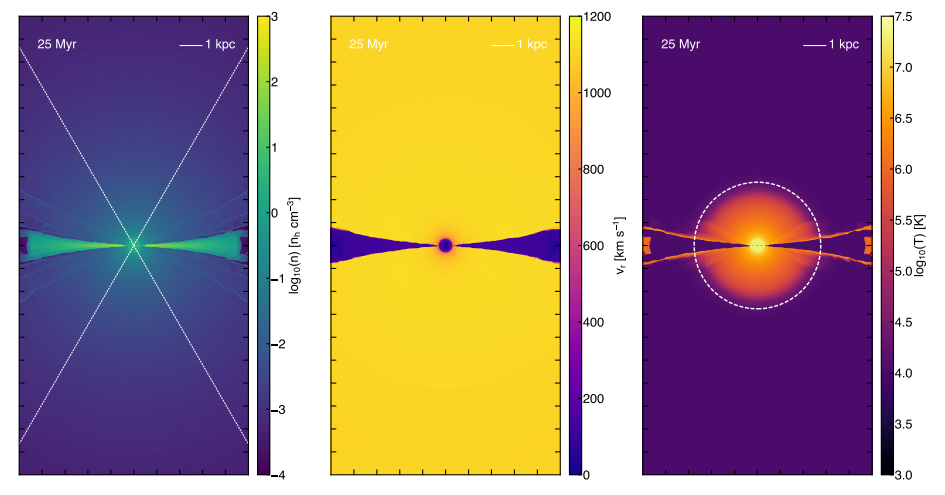
\includegraphics[width=1.0\textwidth]{plots/schneider_uniform.PNG}
    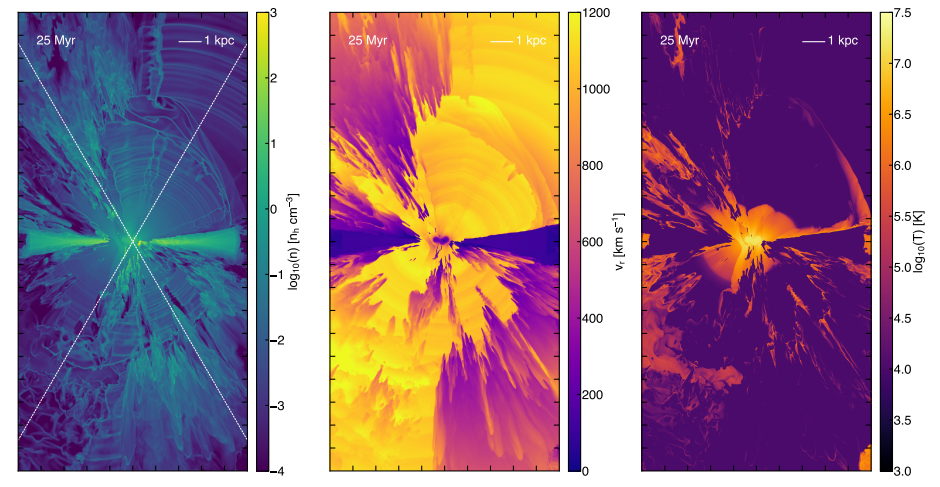
\includegraphics[width=1.0\textwidth]{plots/schneider_cluster.PNG}
    \caption{Snapshots of simulations showing an outflow that undergoes radiative cooling with two different prescriptions for feedback (i.e., energy and mass injections): uniform, central feedback (top panel), and clustered feedback (bottom panel), where energy and mass are injected randomly in small regions inside the galaxy. The galaxy is taken to be a disk, and it is noticeable in the $x - z$ plane's slices. Density, radial velocity, and temperature slices are shown on the left, central, and right panels respectively. The analytically-predicted cooling radius (eq. \ref{eq:rcool}) is plotted as a white dashed circle in the upper-right panel. Taken from Schneider et al. \citep{schneider2018production}.
    }
    \label{fig:thompson_simulation}
\end{figure}




\chapter{The puzzling nature of [CII] halos} \label{chap:halos}
\vspace{20pt}


\begin{comment}

MAIN REFS


TIELENS, DRAINE, PALLO'S AND OTHERS PAPERS,

DALGARNO\&MCCRAY1972?  GOLDSMITH+12?

FUJIMOTO+19, FUJIMOTO+20

MAYBE SOME OTHER REFS -- FRONTIERS OF COSMO LECTURES?

 SAY THAT WE ARE INTERESTED IN HIGH REDSHIFT GALAXIES -- ZOOM IN (PALLO) SIMULAITONS??


SUMMARY 


 1. INTRO TO HIGH REDSHIFT GALAXIES
 
 2. PHYSICAL CONDITIONS IN THE ISM AND CGM
    (PHASES OVERVIEW)
 
 3. EMISSION IN THE ISM/CGM (COOLING/HEATING)

 4. OBSERVATIONAL PROBES OF HIGH REDSHIFT GALAXIEs (OPTICAL; IR)
 
 5. EXTENDED HALOS PROBES
 
 6. HYPOTHESES FOR THE EXTENDED HALOS FORMATION
 
 7. 
 
 8. 
 
 9. 
 
USEFUL THINGS TO MENTION
 - COOLING/HEATING
 - EQUILIBRIUM CONDITIONS, EINSTEIN COEFFICIENTS ETC
 - PHOTOIONIZATION EQUILIBRIUM
 - ISM/CGM PHYSICAL CONDITIONS
 - EXTENDED HALOS OBSERVATIONS
 
\end{comment}




In the first two chapters of this work, we have laid the foundations of our discussion by presenting a summary of the most important topics in galaxy formation and galactic outflows physics. From now on, we focus on the specific problem our thesis work aims to solve. In this chapter, we present this problem by describing the discovery of extended \CII halos in high redshift galaxies. 

In 2019, Fujimoto et al. \citep{Fujimoto19} reported a "First identification of $10$-kpc Scale \CII $158$ $\mu$m Halos around Star-Forming Galaxies at $z=5-7$". By stacking images of $18$ high-redshift galaxies observed by the ALMA interferometer, these authors were able to unveil the presence of emission of the singly ionized carbon line \CII that was much more extended than the stellar continuum UV emission coming from the corresponding galaxies. 

Gaseous halos had already been identified and studied at low redshift, where a much more detailed analysis of the morphology and physical conditions of the CGM is possible (we introduce these halos in section \ref{sec:general_halos}). However, the presence of diffuse extended \CII emission at high redshift is quite surprising, as it raises a series of challenging theoretical questions that do not find a simple answer in terms of low-redshift halos counterparts. For this reason, after presenting the whole body of observational evidence available to date (section \ref{sec:halo_data}), we elaborate on these questions and their possible answers in section \ref{sec:theory_halos}. We summarize the theoretical studies on \CII emission at high redshift, and we describe the results of zoom cosmological simulations. Finally, we list the most promising solutions that aim to describe the origin of these extended halos. We then focus on the hypothesis that halos at high redshift and galactic winds are strongly connected, describing the arguments in favor of this picture and laying the basis for our outflow model that will be the subject of the next chapter. 





\section{Gaseous halos and the CGM} \label{sec:general_halos}


Gaseous halos are formed by baryons residing in the Circum-Galactic Media of galaxies. As already described in section \ref{sec:feedback}, the CGM is the stage where several processes take place: accreting gas mixes with outflows and galactic fountains. Therefore, it is not uncommon to find halos of diffuse gas in the CGM of star-forming galaxies, resulting from the mutual interaction of these different components (figure \ref{fig:cgm_cartoon}). Several observational techniques can reveal the presence and the properties of these diffuse gas in galaxies' halos \citep[for details, see][]{tumlison}:
\begin{itemize}
    \item Absorption lines in quasars provide information about the objects standing in the QSOs line of sights. Viewing the CGM of a galaxy in absorption against a bright background quasar offers the possibility to explore a wide range of densities - as absorption's measurements have a very high sensitivity - as well as redshifts and luminosities. However, such a technique provides only partial information on the physical conditions of the gas, as it gives only a single, point-like, estimate of the gas surface density. Stacking many different spectra is also a possibility, as it beats down statistical noise, thus enabling measurements of weaker absorbers; however, properties of single systems are averaged out, and physical information such as kinematics and ionization states is thus lost.
    \item Alternatively, a different technique, known as "down-the-barrel" spectroscopy, uses a galaxy’s own starlight as a background source for detecting absorption. This method is commonly used in optical and near-UV lines, to study outflows and/or inflows in low redshift galaxies. The advantage of using down-the-barrel spectroscopy is that it provides key information on the physics of the near-CGM, which is the most interesting region from a physical perspective and it is rarely captured by QSOs absorption studies. An important limitation, however, is that the galactocentric radius of any detected absorption cannot be constrained.
    \item A third possibility is to search directly for light emitted by CGM gas. This emission, scaling as $n^2$, is very challenging to detect. However, this has been done both in nearby galaxies and in higher-redshift ones, probing UV/optical and sub-millimeter wavelengths. Emission maps have the advantage that they can constrain the density profile, morphology, and physical extent of the CGM gas much more in detail than other techniques based on absorption lines. In section \ref{sec:halo_data}, we focus on observations of emission lines in the CGM of high-redshift galaxies.
\end{itemize}
The general picture that emerges from CGM observations hints at a multiphase and dynamically complex structure, hosting a significant fraction of the baryons' budget. The discussion here echoes in many ways the one presented in the context of galactic winds (section \ref{sec:multiphase}): different species probe the presence of many phases characterized by a variety of temperatures and ionization states. A cold and neutral phase ($T\lesssim 10^4\,\mathrm{K}$) coexists with a warmer phase ($T\sim10^{4-6}\,\mathrm{K}$), as well as with hot ionized gas ($T\gtrsim 10^7\,\mathrm{K}$). Evidence for kinematic complexity is then exhibited by the presence of many features in the absorption lines of ions, with different velocities and linewidths. Finally, from the density profiles of CGM gas, the total mass of different phases can be inferred. With this respect, both observations and simulations agree on the fact that the CGM contains a total mass of baryons which is of the same order of magnitude as galaxies' stellar masses. This may contribute to explain why the percentage of baryons residing in stars or in the ISM of galaxies is significantly lower than the one in the IGM (the so-called \textit{missing baryons} problem). An analogous problem concerns the galactic budget of metals (\textit{missing metals}), which can be explained by taking into account the relatively high metallicity of the CGM \citep[e.g.,][]{lehner2018}. 


The analogy we have made with outflows is not accidental. Indeed, one of the major candidates for producing the extended, multiphase CGM is the mixing between the halo gas and galactic winds that continuously takes place as gas flows out of the galaxy \citep{Thompson16,fielding2017impact}. Other scenarios include the presence of cooling inflows driven by thermal instabilities \citep{mccourt2012thermal}, and cool clouds entrained in outflowing/inflowing gas (for more details, see section \ref{sec:outflows_cooling}). Disentangling the relative contributions of these mechanisms is not an easy task, as distinguishing between inflows and outflows is only partially possible. Observations, however, indicate that outflows have a greater covering factor \citep{rubin2014evidence}, suggesting that a large part of the CGM is made of outflows.  


\begin{figure}
	\centering
	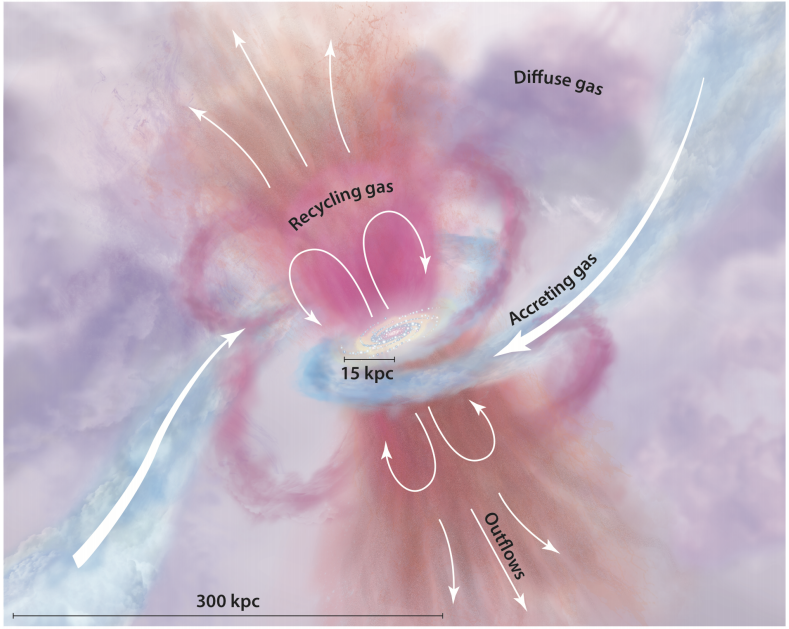
\includegraphics[width=0.6\textwidth]{plots/cgm.PNG}
	\caption{A sketch of the different gas components populating the CGM of a star-forming galaxy. Outflowing/recycling gas is represented in pink and orange, while gas accreting from the IGM has a light blue shade. Tones of purple highlight the presence of diffuse gas in the halo whose source is mixed or unclear. Taken from Tumlinson et al. \citep{tumlison}.
	}
	\label{fig:cgm_cartoon}
    \end{figure}


\section{Observations of halos at high redshift} \label{sec:halo_data}


The discussion presented in the last section provides a partial but reasonable picture of the conditions of the CGM in local and low redshift galaxies. However, in the last few years, new observational capabilities have paved the way to the study of galaxies deep into the Epoch of Reionization ($z\approx6$; see section \ref{sec:first_lights_reionization}). Reionization marks the epoch at which galaxies are still evolving at a fast rate, and start to alter the ionization state of the IGM. Therefore, in this epoch, galaxies are expected to have different morphologies, physical and chemical properties from their local counterparts. For this reason, observations of high redshift galaxies are particularly interesting, as they offer the opportunity to trace back the galactic evolution process, and to shed light on the mechanisms of interaction between galaxies and the pristine medium surrounding them. 

High redshift observations differ from local ones for a variety of reasons. Most importantly, cosmological redshift moves radiation from stars and galaxies in different regions of the electromagnetic spectrum. For redshifts $z\approx 4-7$, UV and optical radiations are shifted to the Near-InfraRed (NIR), while dust emission gets shifted further into the FIR/millimeter wavelengths. Therefore, investigating galaxies in the NIR can offer important information on the light emitted by stars that is not absorbed by dust (i.e., it can probe the so-called \textit{unobscured star formation}). On the other hand, looking at the FIR completes the picture by providing details about the \textit{obscured star formation}. Emission and absorption lines in these two regions of the electromagnetic spectrum can also be used in synergy to study the kinematics, composition, temperature, and density of gas in the ISM/CGM of high-redshift galaxies. This kind of \textit{panchromatic surveys} are routinely used in the local universe, but they have become possible even at higher redshift thanks to the synergy between space telescopes such as the Hubble Space Telescope (HST) and Spitzer and ground telescope such as the Very Large Telescope (VLT), the Atacama Large Millimeter/submillimeter Array (ALMA), and the NOrthern Extended Millimeter Array (NOEMA). 

In particular, the rest-frame UV/optical part of the spectrum has been probed multiple times in the last decade using spectroscopic and imaging surveys \citep[e.g.,][]{oesch2009structure,Shibuya:2015qfa, bouwens2017z, kawamata2018size}. Thanks to these studies, we have now a solid statistical sample that can gauge the evolution of several properties in high redshift galaxies, such as the UV-luminosity function, the size and morphology of the stellar and gaseous components, and the unobscured star formation history. Information from the dust and cold gas emitting in the FIR band, instead, has become available only thanks to the advent of radio-interferometers such as ALMA and NOEMA. In the last few years, these instruments have offered the opportunity to measure continuum (thermal) emission from dust in high redshift galaxies, as well as emission lines from cold ISM gas such as [CII] $158 \,\mu\mathrm{m}$, [O III] $88 \,\mu\mathrm{m}$, and CO from various rotational levels \citep{maiolino2015,capak2015,pentericci2016,knudsen2016b, matthee2017, carniani2018b, Hashimoto2018,gallerani:2018}.

In this work, we focus on spatially-resolved ALMA observations of the \CII line in galaxies at $z\approx 4-7$. The \CII line is created by the fine-structure transition $^2P_{3/2} \rightarrow
\,^2P_{1/2}$ of singly ionised carbon at $\lambda = 158\,\mu\mathrm{m}$. It is one of the brightest lines in the FIR, as it accounts for a significant fraction ($\approx 0.1-1\,\%$) of the total FIR luminosity \citep{gong2012}. Being also very easy to excite, it arises from gas with very different physical properties. We discuss in more detail the theoretical models that describe \CII emission in section \ref{sec:theory_halos}. 

By comparing the spatial extension of \CII with the extension of rest-frame FIR and UV emission, a growing number of works \citep{carniani2018b, Fujimoto19, ginolfi:2019, Fujimoto:2020qzo, herrera2021kiloparsec} have found that the \CII emitting region of galaxies at high-z is significantly more extended than the continuum one. These findings pair with parallel evidence for the presence of extended Ly$\alpha$ line emission at high redshift: as found by e.g., \citet{Wisotzki16}, the effective radius of the Ly$\alpha$ spatial extension on average $\sim 5-15$ times more extended than the central UV continuum. 

As the UV/FIR continuum traces the stellar region - and hence the size of the galaxy - the presence of extended \CII (Ly$\alpha$) emission probes the presence of singly ionized carbon (neutral hydrogen) deep into the CGM of normal star-forming high-z galaxies. In turn, this has profound implications on our understanding of galaxy formation and evolution. Carbon, in particular, plays a key role in this discussion, as it witnesses early gas exchanges between galaxies and their CGM. In fact, while diffuse metal halos at low redshift are compatible with our understanding of feedback and accretion (section \ref{sec:general_halos}), the presence of these extended structures at high-z implies very early contamination of the pristine CGM by the products of stellar nucleosynthesis. Moreover, the ionization state of carbon implied by the presence of massive \CII emission can offer us very important information on the density, temperature, and radiation fields acting on the gas in the surroundings of early galaxies. In the next few paragraphs, we describe in detail the whole body of observations of \CII halos available to date. Theoretical considerations and physical implications of these observations are left for the last section.  






\subsection{First identification}

Early signs of the presence of \CII extended emission at high redshift were found by Cicone et al. \citep{cicone2015} in a massive $z\sim6$ quasar host, using observations taken with the IRAM Plateau de Bure Interferometer (the precursor of NOEMA). By measuring the spatial extent of the \CII line and of the FIR continuum, the authors proved that the former reaches a maximum projected radius of $30$ kpc, while the latter does not exceed $15$ kpc. This extended emission is likely associated with a powerful AGN-driven outflow, as a large part of the gas traced by \CII is at high velocities (i.e., up to $\sim 1400\,\kms$ relative to the systemic velocity). 

The higher sensitivity of ALMA opened up the study of normal star-forming galaxies at the same redshifts. With this respect, a first work by Carniani et al. \citep{carniani2018} used archival ALMA observations to study the properties of \CII emission in normal $z\approx 5-7$ galaxies. They revealed that, in their sample of $29$ galaxies, \CII emission is generally much more extended than the UV emission. However, a similar result needed to be supported by further analyses, as a low signal-to-noise ratio (S/N) and large uncertainties could undermine the reliability of size measurements. 

The work of Fujimoto et al. \citep[][hereafter F19]{Fujimoto19} confirmed the presence of extended \CII halos by stacking several observational data in order to increase the S/N. In the F19 paper, the authors identify in the literature \citep[e.g.,][]{capak2015, maiolino2015, willott2015, pentericci2016, carniani2018} 18 galaxies at $z \approx 5-7$ that met some specific requirements, such as \CII S/N$>5$, no signs of AGN activity or gravitational lensing, SFR$<100\,\msun\mathrm{yr}^{-1}$, \CII line with a Full-Width Half Maximum (FWHM) broader than $80\,\kms$. Using this sample of galaxies, a stacking technique in the $u-v$ visibility plane (i.e. the 2-d transform of the sky brightness plane) is applied to obtain a single emission map with an effective S/N of $21$ and $10$ for the \CII line and the dust continuum respectively. UV continuum HST observations of the same galaxies are stacked as well, and the HST Point Spread Function (PSF) is convolved with a best-fit kernel in order to make it equivalent to the ALMA beam. In this way, a fair comparison between ALMA and HST spatial emission data is possible. 

The left panel of figure \ref{fig:fuji_data} represents the final spatial emission maps of \CII, FIR and UV continuum obtained by following the stacking procedure. On the right panel, the averaged radial profile for these quantities is shown: from this plot, it is easy to conclude that the \CII emission (red) is much more extended than the (rest-frame) FIR and UV ones (green and blue respectively). This result implies that $10$-kpc scale \CII halos surround star-forming galaxies in the early Universe. The existence of these halos is statistically significant at the $9.2\sigma$ level. Exponential fits of the halo profile, as well as of the HST stellar continuum, show that the scale length of the \CII is a factor of $\sim5$ times greater than the continuum's one. This is in agreement with the fact that the typical radius of normal star-forming galaxies at $z\approx 6$ is estimated to be less than $1$ kpc \citep{Shibuya:2015qfa}. Overall, the F19 analysis is the first strong statistical evidence in favor of the existence of extended \CII halos in the CGM of high redshift galaxies.




\begin{figure}
    \centering
    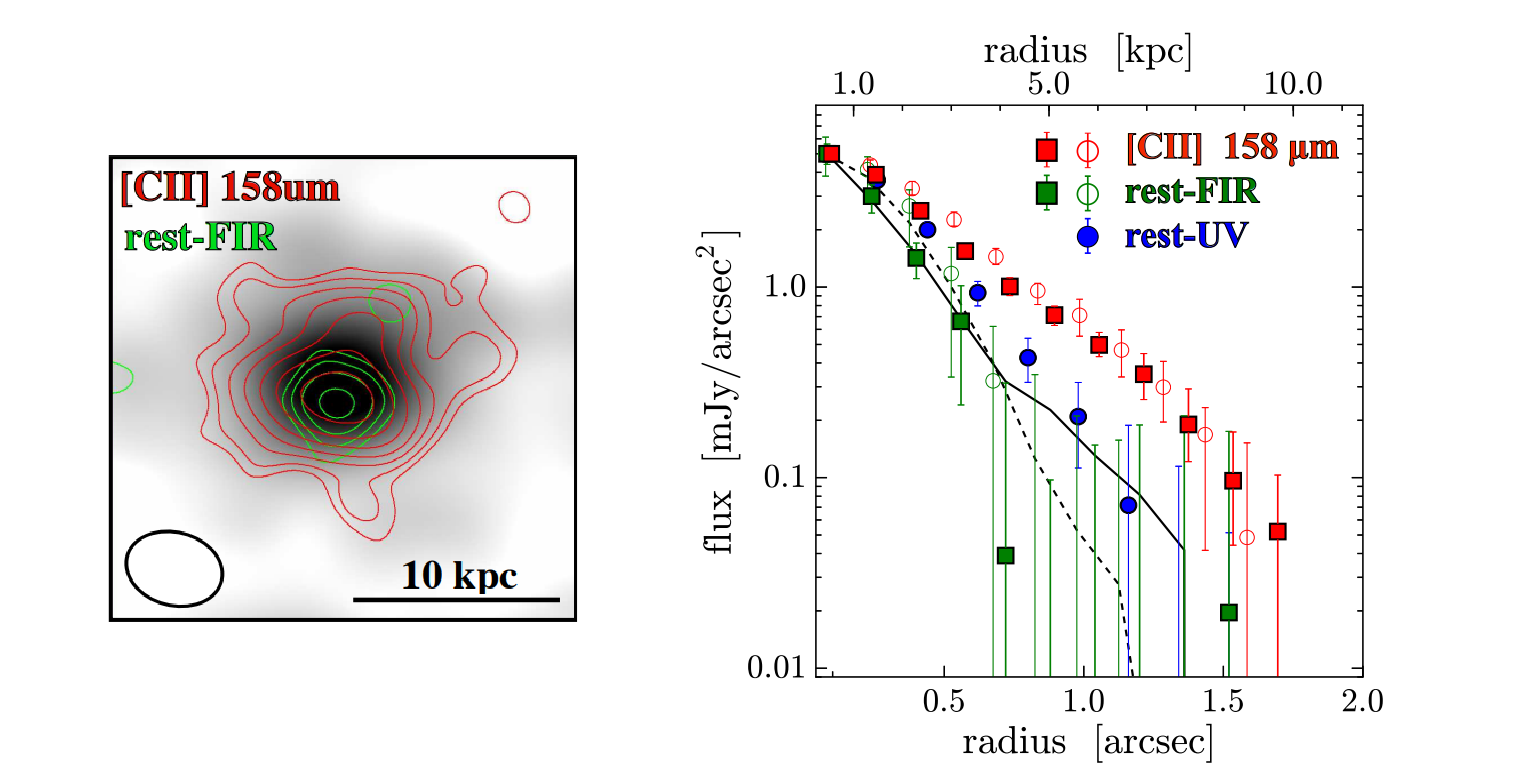
\includegraphics[width=1.0\textwidth]{plots/fuji_data_final.png}
    \caption{\textit{Left:} spatially resolved emission maps taken from F19 \citep{Fujimoto19}. The background image shows the rest-frame UV emission (whose resolution is matched to the ALMA image), while the red and green contours show the \CII line and the (FIR) dust continuum emission respectively. \textit{Right:} averaged radial surface brightness profiles for the F19 \citep{Fujimoto19} sample. The red, green, and blue symbols denote the \CII line, rest-frame FIR, and rest-frame UV continuum emission respectively. Square symbols refer to the whole sample, while circles only include the galaxy for which the HST continuum images are available. The black dashed and solid curves denote the ALMA synthesized beams for these two sub-samples. All radial profiles are normalized to the peak value of the \CII line. 
    }
    \label{fig:fuji_data}
\end{figure}


\begin{figure}
    \centering
    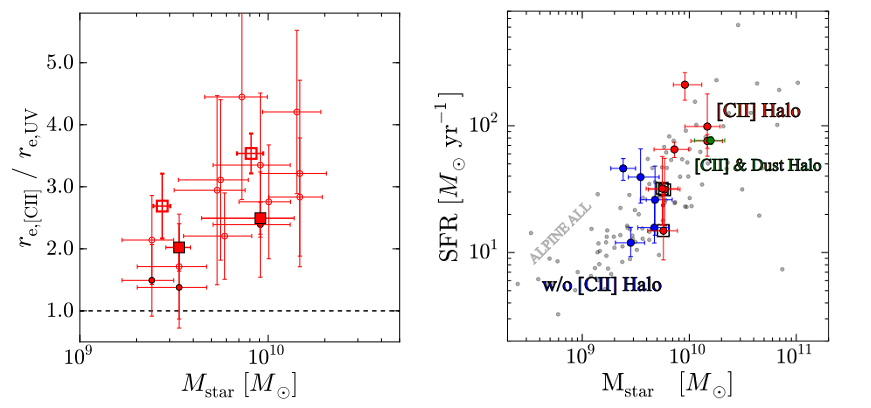
\includegraphics[width=1.0\textwidth]{plots/alpine_effective_radius_final.png}
    \caption{\textit{Left:} ratio of $r_{e,\mathrm{CII}}$ to $r_{e,\mathrm{UV}}$ as a function of the stellar mass $M_\mathrm{star}$ taken from the F20 \citep{Fujimoto:2020qzo} study. The rest-frame UV sizes shown with the open and filled shapes are estimated from the HST F814W and F160 maps, respectively. The circle symbols are the actual data, while the squares represent the median values in bins of $M_\mathrm{star}$. \textit{Right:} scatter in the SFR vs $M_\mathrm{star}$ plane for the sample of ALPINE galaxies (grey dots), taken from F20 \citep{Fujimoto:2020qzo}. Sources labeled as "\CII Halo", "without (w/o) \CII Halos", and "\CII \& Dust Halo" (see text for the definitions) are highlighted using red, blue, and green circles respectively.
    }
    \label{fig:alpine_trends}
\end{figure}


\subsection{Results from the ALMA ALPINE program} \label{sec:alpine}


A few months after the release of the F19 study, the ALPINE ALMA observational data became available \citep{lefevre:2019, faisst:2019, bethermin:2019}. ALPINE (ALMA Large Program to INvestigate C+ at Early Times) is a $69$-hours large ALMA program that started in May 2018 and ended in February 2019. The goal of the program was to explore the gas and dust FIR properties in 118 normal star-forming galaxies at $4.4 < z < 5.9$. For this reason, these galaxies were observed in ALMA Band 7, where the \CII line resides, at a spatial resolution of $\lesssim 1.0''$. The galaxies origin from two fields: the Cosmic Evolution Survey field (COSMOS, \citep{scoville2007field}) and the Extended Chandra Deep Field South (ECDFS, \citep{giacconi_field}). All galaxies are spectroscopically confirmed by either Ly$\alpha$ emission or rest-UV absorption
lines, and they are selected to be brighter than an absolute UV magnitude of $M_{1500} = -20.2$. Observations of the rest-frame UV to optical bands with Keck, VLT, HST, and Spitzer are available, and thus a good amount of ancillary data can complement ALMA observations, giving good estimates of the galaxies' (unobscured) SFR and of their stellar mass. The sample has SFRs between $10\,\msun\mathrm{yr}^{-1}$ and $500\,\msun\mathrm{yr}^{-1}$, and masses in the range $M_* \sim 10^9 - 10^{11} \,\msun$. At the end of the program, \CII line was detected above the $3.5\sigma$ level in $64\%$ of the galaxies, while the FIR continuum detection rate was $19\%$.


\begin{figure}[t]
    \centering
    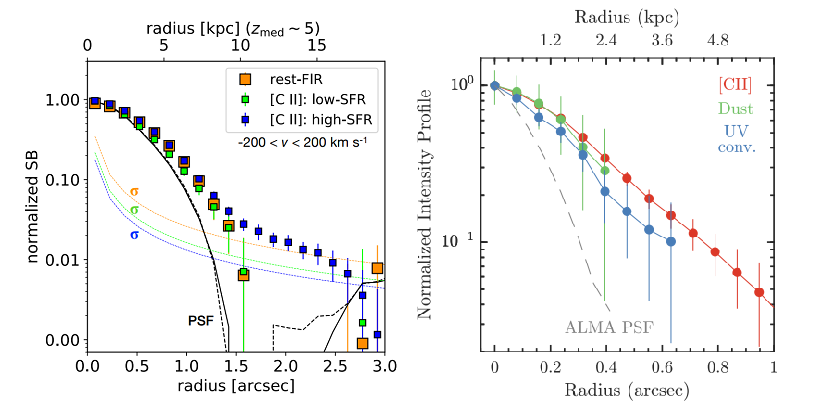
\includegraphics[width=1.0\textwidth]{plots/ginolfi_hc_final.png}
    \caption{\textit{Left:} averaged radial profiles taken from the G19 \citep{ginolfi:2019} stacking analysis; the \CII emission in the $[-200:+200]\,\kms$ range is shown in green squares for the low-SFR sample ($\mathrm{SFR}<25\,\msun\mathrm{yr}^{-1}$), and in blue squares for the high-SFR one ($\mathrm{SFR}>25\,\msun\mathrm{yr}^{-1}$). Orange squares represent the rest-frame FIR continuum, while the solid and dashed black lines represent the ALMA PSF for the whole sample and the continuum-detected sub-sample. \textit{Right}: averaged and normalized radial intensity profiles taken from the HC21 \citep{herrera2021kiloparsec} work. \CII emission (red), rest-frame FIR (dust) continuum (green), and convolved rest-frame UV continuum emission (blue) are shown, as well as the ALMA beam (dashed grey line).
    }
    \label{fig:alpine_data}
\end{figure}

The scientific goals of ALPINE perfectly align with the problem of characterizing the CGM in high redshift galaxies. In particular, spatially resolved emission of the \CII line was obtained for all the galaxies where \CII was detected. These data can provide information on extended halos at a much higher sensitivity than before, allowing a study of halo-hosting galaxies at the individual level, as well as a statistical characterization of their properties. Between 2019 and 2020, two studies presented the results of ALPINE in the context of extended \CII halos. The first one, Ginolfi et al. \citep[][hereafter G19]{ginolfi:2019}, selected a sub-sample of $50$ ALPINE galaxies whose \CII line was detected above a S/N threshold of $5$, and applied stacking procedure both to the \CII line spectra and to the \CII line data-cubes (i.e., the \CII spatial emissions as a function of the wavelength/radial velocity). Their results are particularly interesting, as both of the stackings yield important information on the properties and nature of \CII halos. Stacking the data-cubes and integrating over a $-200\,\kms<v<200\,\kms$ velocity range, they find clear evidence for a \CII structure extending out to the $15\,\mathrm{kpc}$ scale. Considering the spectra, instead, they detect broad-wings features at velocities of few hundreds of $\kms$. These are typical signatures of outflows, as they are created by high radial velocity gas, whereas the central Gaussian component originates from the kinematics of the gas bounded to the central galaxy. Therefore, these findings suggest that both outflows and extended halos are a common feature of star-forming high-z galaxies: this thesis work aims to causally connect these two pieces of evidence by providing a model for an outflow that is able to account for the observed \CII extended emission. 

Another compelling finding from G19 is the dependence of the halo's extension and outflow's features on the star formation rate. By dividing the ALPINE sample into two sub-samples with $\mathrm{SFR}<25\,\msun\mathrm{yr}^{-1}$ and $\mathrm{SFR}>25\,\msun\mathrm{yr}^{-1}$ respectively, they find that the broad-wing feature indicating ongoing outflow activity is much stronger for the high-SFR sub-sample, and that only this latter group of galaxies show the extended halo feature, while the rest of low-SFR galaxies does not show any \CII emission outside the FIR continuum region (figure \ref{fig:alpine_data}). A similar trend is a clear indication that both the observed outflows and the extended \CII structures are created by SF-related processes. We have already described (chapter \ref{chap:outflows}) how outflows can be driven by star formation via the energy and momentum released by SNe and stellar winds. In the next chapter, we argue for a picture where these same SF-driven outflows are responsible for the \CII halos formation.


A second study by Fujimoto et al. \citep[][hereafter F20]{Fujimoto:2020qzo}, then, analyzed the ALPINE sample searching for signatures of \CII halos on the individual level. The authors consider only the ALPINE galaxies that were detected in \CII above $5\sigma$ and that were not classified as mergers by a visual inspection of their morphologies. In this way, only galaxies whose \CII emission is strong and not spuriously created by companions are selected. For every galaxy in this subsample, they use an exponential profile to fit the emission both in \CII and in the rest-frame UV continuum (from HST data). They obtain two effective radii, $r_{e,\mathrm{CII}}$ and $r_{e,\mathrm{UV}}$, representing the extension of the \CII and stellar regions respectively (see the F20 paper \citep{Fujimoto:2020qzo} for details on the fitting procedure). 

Figure \ref{fig:alpine_trends} (left panel) shows the ratio $r_{e,\mathrm{CII}} / r_{e,\mathrm{UV}}$ as a function of the galaxy stellar mass (only measurements that are considered as reliable are shown in the plot). The ratio stays always in the range $2-3$, meaning that the effective size of the \CII region is consistently greater than the UV one. Moreover, there is a clear trend with stellar mass, meaning that the relative size of the \CII extended region is bigger for higher stellar masses. 

In order to investigate this result more carefully, F20 considers the full (averaged) radial profiles for \CII, UV-continuum (from HST), and (when available) FIR-continuum. Matching the resolution of these different quantities -- simply convolving the ALMA profiles with the HST beam and vice-versa --, they obtain emission maps and radial profiles for individual galaxies. Then, they classify these galaxies in three different categories, by looking at the strength of the \CII, FIR, and UV emissions in a "peripheral region" obtained by masking a central area corresponding to the observational beam. A galaxy is defined to host a \CII halo if the statistical significance of the \CII emission in this peripheral region is above the $4\sigma$ level, and, at the same time, the statistical significance of the UV and FIR emissions are below $3\sigma$. Similarly, a galaxy is defined as "without \CII halo" if the statistical significance in this region is below $3\sigma$ for all the \CII, FIR, and UV emissions. 

F20 identifies seven sources (DC$396844$, DC$630594$, DC$683613$, DC$880016$, DC$881725$, VC$5100537582$, and VC$5110377875$) hosting a "CII halo", and six other galaxies not showing signs of extended \CII emission. A third category ("\CII \& Dust halos") is also created for the only object (DC$488399$) showing signs of extended emissions both in \CII and FIR (i.e., dust continuum), but not in UV. Figure \ref{fig:alpine_halos} represent some instances of emission maps and radial profiles for sources hosting a \CII halo, without a \CII halo, and with the \CII \& Dust halo. 

Overall, F20 finds that $\sim 30\%$ of the sources have a \CII halo extending over $15-\mathrm{kpc}$ scales. Note that this number may be even higher, as observational limitations could in principle hamper the identification of fainter halos in the remaining part of the sample. Deeper observations are needed to test whether \CII halos are ubiquitous in normal star-forming galaxies, or form only in a part of them.

Having set a lower bound to the number of galaxies hosting a \CII halo, the authors in F20 can then compare them to the full ALPINE sample, in order to identify some specific features that are correlated with the presence of extended \CII emission. The most significant correlations they find are shown in figure \ref{fig:alpine_trends}, where the distribution of the ALPINE sample in a SFR vs stellar mass scatter plot is displayed. \CII halos (w/o \CII halos) galaxies are highlighted in red (blue) circles. Halo-hosting objects are clearly biased towards higher masses and higher SFR. 

This result is consistent both with the effective radii trend discussed in figure \ref{fig:alpine_trends} and with the result from the ALPINE stacking presented in G19. As already discussed, this could imply a role of star formation in the halos formation process. However, we have to keep in mind that if observational constraints are preventing fainter halos to be observed, then these trends could be simply due to selection biases. On the other hand, there are few sources with similar SFR and $M_\mathrm{star}$ but different halos properties, suggesting that these trends are at least partially valid. 

After completion of the ALPINE program, another observational study by \citet[][hereafter, HC21]{herrera2021kiloparsec} made some important steps forward in the study of \CII emission in normal high-z galaxies. The authors of the study used the ALMA telescope to perform a follow-up observation of the ALPINE system DC$494057$ (also known as HZ$4$) with very high ($\approx 0.3''$) spatial resolution. This system was not part of the F20 "\CII halo" category. However, thanks to the increased resolution of the HC21 study, it has been possible to find strong statistical evidence for the presence of a \CII halo surrounding the HZ$4$ galaxy. The halo extends beyond the star-forming disk and has a radius of $\approx 6$ kpc. Figure \ref{fig:alpine_data} (right panel) shows the averaged radial profiles for the \CII line and the UV/(FIR) emissions. 

Furthermore, the high observational resolution of the HC21 has another key advantage, as it allows to resolve the central regions of the galaxy and to isolate single regions of $\approx 2$ kpc size. Studying the spectral properties of these regions on an individual basis, the authors have found evidence for an outflow that extends from the central regions of the galaxy in the direction of its minor axis. The outflow has a velocity in the range $v\approx 320-420 \kms$ -- consistent with velocities
measured in lower redshift systems -- and a local mass loading factor (section \ref{sec:obs_outflows}) equal to $\eta \approx 3-6$. Overall, these findings seem to suggest that the outflow and the carbon halo are -- at least partially -- causally connected.

\begin{figure}
    \centering
    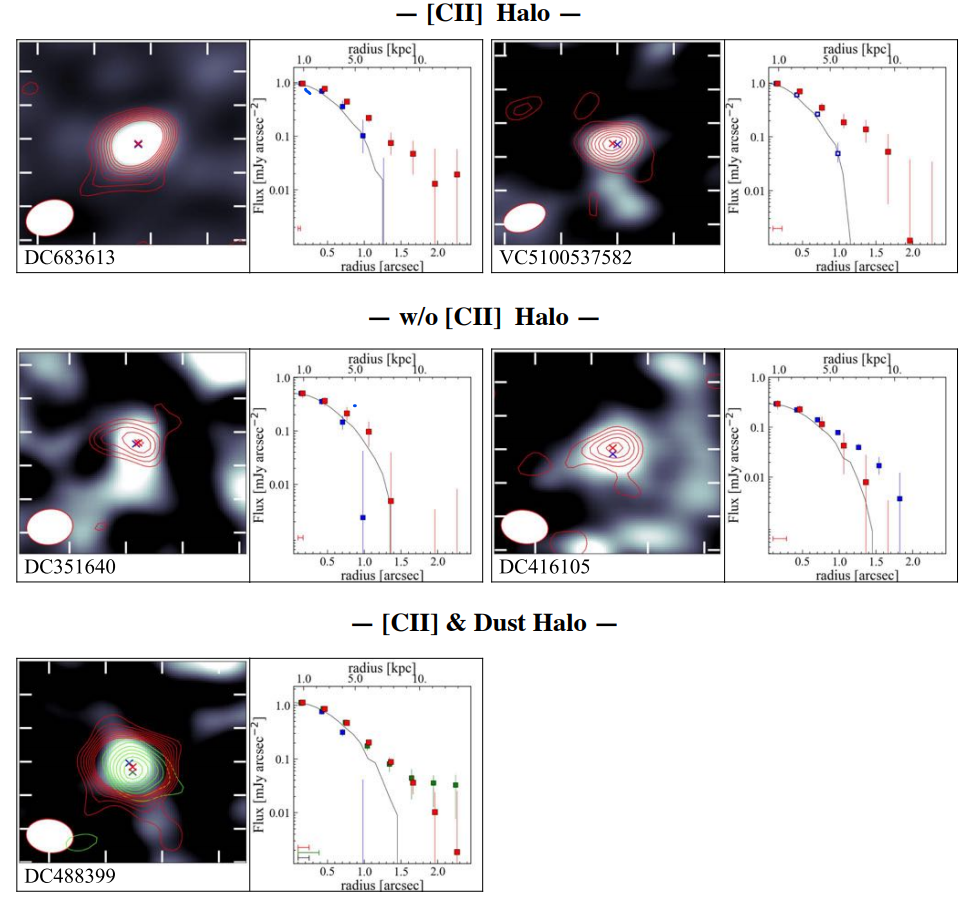
\includegraphics[width=1.0\textwidth]{plots/alpine_halos.png}
    \caption{Instances of ALPINE individual galaxies analyzed in F20 \citep{Fujimoto:2020qzo}. The objects are divided into three categories, as described in the text: "\CII Halo", "without (w/o) \CII Halo", and "\CII \& Dust Halo". On the left panels, the spatial distributions of the \CII line (red), the rest-frame FIR (green, wherever available), and UV continuum (background) are shown. The HST image and ALMA contours are smoothed by the ALMA synthesized beam and the HST PSF, respectively, to match the spatial resolutions between the HST and ALMA maps. Right panels show the averaged radial surface brightness profiles for the \CII line (red squares), the rest-frame FIR (green squares) and UV (blue squares) continuum. The black solid curve shows the ALMA synthesized beam. All profiles are normalized to the \CII one. 
    }
    \label{fig:alpine_halos}
\end{figure}



\section{Insights from theory and simulations} \label{sec:theory_halos}


The body of observational data that has piled up in the last few years poses the existence of \CII halos on very solid ground. For this reason, it is important to interpret the presence of these halos in light of current cosmological models for galaxy formation and evolution. In recent years, several studies have focused on modeling the physical conditions in the ISM and CGM of high-z galaxies, with particular focus on the problem of \CII emission. We briefly review the role that \CII is thought to play in high redshift systems, in order to present the theoretical questions arising from the discovery of \CII halos in the right context. Then, we look at the most promising solutions that may be able to give an answer to the halos problem.

\subsection{[CII] emission in high-z galaxies} \label{sec:CII_models}




The gas in the ISM of galaxies is organized in a variety of phases \citep{tielens2005book}: cold clouds coexist with a hot intercloud medium, as well as with a warm medium, divided in neutral and ionized. These diffuse and low-density components are often accompanied by denser regions, that take different names based on their temperature and composition. \HII regions are made by warm, ionized gas, while (giant) molecular clouds are composed of neutral gas and molecules, and they have a temperature as low as $10\,\mathrm{K}$ (see also sec. \ref{sec:first_lights_reionization}). Photo-dissociation regions (PDR) arise in the outer layers of molecular clouds, where Far-UV radiation (with energy in the range $6-13.6\,\mathrm{eV}$) can penetrate inside because it is not absorbed by neutral hydrogen; as a results, trace species such as carbon and silicon -- whose ionization potential is lower than $13.6\,\mathrm{eV}$ -- become ionized.


The $158\,\mu\mathrm{m}$ \CII emission arises primarily in PDR regions \citep{hollenbach1999}. However, given that its line transition is very easy to excite ($E/k \approx 92\,\mathrm{K}$), it can also trace the diffuse (cold and warm) neutral medium \citep{wolfire2003}, and to a lesser degree even the ionized medium \citep{cormier2012}. The ubiquity of \CII emission makes it one of the major coolants in the ISM, and the brightest line in the FIR window. At high redshifts ($z\gtrsim 4$), this window is conveniently redshifted to sub-millimeter wavelengths, where it can be detected with earth-based telescopes \citep{bethermin:2019}. For this reason, several theoretical studies have focused on determining the relative contribution of different ISM/CGM phases to the \CII luminosity \citep{vallini2015, pallottini2017, pallottini:2019}, as well as the role of gas dynamics \citep{kohandel:2019} and star-formation \citep{vallini2017, ferrara:2019} in the physics governing the \CII emission at high redshifts.

These studies are often base on zoom simulations: a cosmological simulation (sec. \ref{sec:physics_galaxies}) is set up in order to resolve one or more specific systems, reaching a spatial resolution as low as $10\,\mathrm{pc}$ \citep[e.g.][]{pallottini:2019}. With this resolution, the ISM thermochemical non-equilibrium evolution can be followed, including the contribution of chemical, radiative, and mechanical feedback from star formation. \CII emission is usually computed in the post-processing phase, coupling radiative-transfers schemes with physically motivated prescriptions for the ISM. Simulations and other theoretical results agree on the fact that most of the total \CII luminosity arises from the dense PDRs, with little contribution from the diffuse medium \citep[e.g.,][]{vallini2015, pallottini2017}. 


The \CII luminosity profiles predicted by simulations can be compared with the observed extent of \CII emission. Quite surprisingly, even recent and most physically rich zoom simulations fail to reproduce the observed \CII profiles. This is shown in figure \ref{fig:simulations_halos}, by comparing results from F19 \citep{Fujimoto19} with simulations from \citet{pallottini2017b} and \citet{Arata:2019}. These two independent studies agree in predicting a \CII emission that is slightly more extended than the stellar continuum but drops very rapidly at distances considerably smaller than $10\,\mathrm{kpc}$. The resulting profiles are characterized by a value of the surface brightness which, in the external regions, is at least one order of magnitude lower than observed. This mismatch between theory and observation hints either at a non-optimal choice of the parameters governing numerical implementations, or at the presence of some undergoing physical process that has not been completely captured by theoretical models. 


\begin{figure}[t]
    \centering
    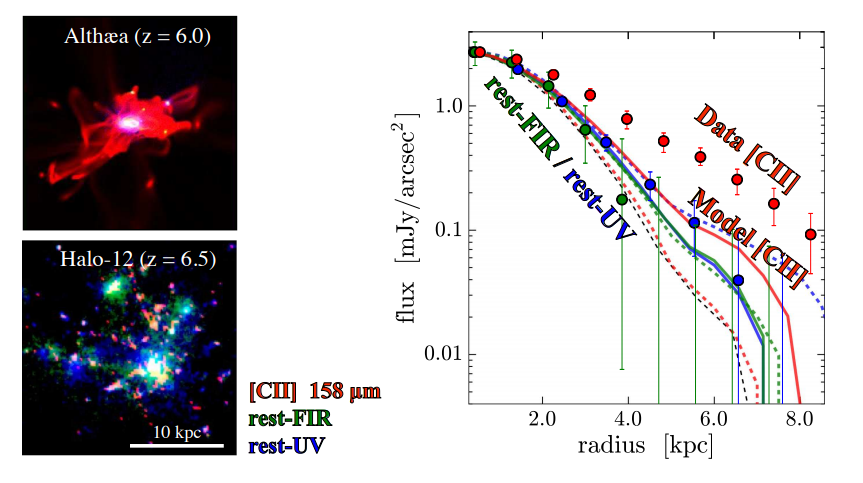
\includegraphics[width=0.85\textwidth]{plots/pallo_sim_halos.PNG}
    \caption{\textit{Left panel}: $4''\times4''$ fake-color image for Althaea (top) and Halo-12 (bottom), obtained from the zoom simulations presented in \citet{pallottini2017} and \citet{arata2019radiative}, respectively (red: \CII line; green: rest-frame FIR continuum; blue: rest-frame UV continuum). \textit{Right panel}: radial averaged surface brightness profiles for the \CII line (red curve), rest-frame FIR (green curve), and UV (blue curve) continuum emission, obtained by stacking the profiles from zoom simulations. The solid and dashed color lines present the Althaea and Halo-12 results, respectively. The black dashed curve denotes the ALMA synthesized beam. Circles indicate the measured profiles obtained by the F19 stacking \citep{Fujimoto19} (same as figure \ref{fig:fuji_data}, left panel). Figure taken from F19 \citep{Fujimoto19}.
    }
    \label{fig:simulations_halos}
\end{figure}

\subsection{Open questions and candidate solutions}

\begin{figure}
    \centering
    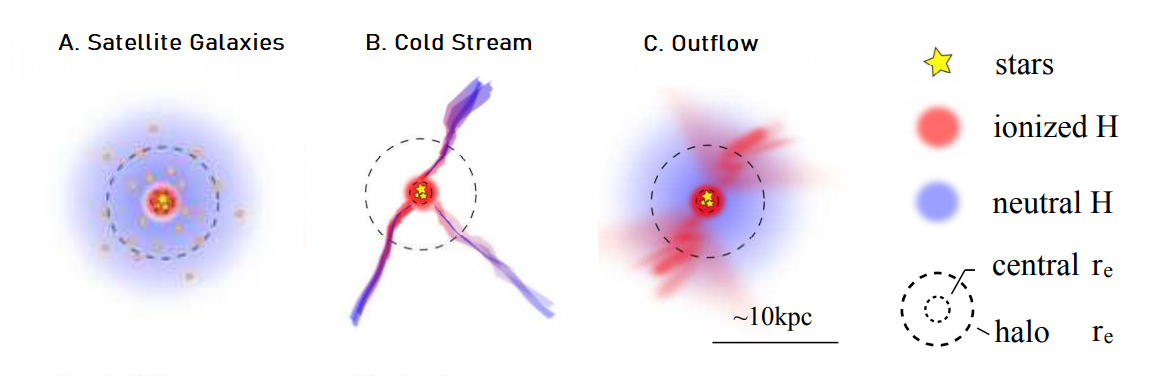
\includegraphics[width=1.0\textwidth]{plots/solutions_final.png}
    \caption{Sketches of three possible scenarios for the physical origin of the \CII halos: A) satellite galaxies; B) cold streams; and C) outflows. Neutral (ionized) hydrogen in the ISM and CGM is shown in blue (red), while yellow stars represent the star-forming regions. The inner and outer dashed circle denote the effective radii ($r_e$) of the central and \CII halo components, respectively. Figure adapted from F19 \citep{Fujimoto19}.
    }
    \label{fig:solutions_halos}
\end{figure}

From the discussion presented in the last paragraphs, it is clear that explaining the origin of extended halos at high redshift, as well as investigating their evolution over cosmic time, is a formidable problem in galaxy evolution. In particular, a number of questions need to be addressed by any theoretical arguments aiming to solve the puzzle of \CII halos:
\begin{itemize}
    \item First of all, the presence of carbon (and presumably other heavy elements) far away from the center of the galaxy questions current models of galaxy evolution. In fact, at high redshift, the gas composing the CGM/IGM of galaxies is expected to have a very low metallicity, since metals are formed only by stars in the central regions of the galaxies. The presence of significant carbon emission implies that carbon has had to be either transported away from the galaxy or created by hidden star-formation activity in the external galactic environment. By what means, then, has carbon been transported to these large distances from the galactic center? How is it present in such a massive amount in the CGM of galaxies?
    \item Even if enough carbon is present in the halo region of galaxies, there is no guarantee that \CII emission matches the observed one. That is because, as we have summarized in section \ref{sec:CII_models} and as we will elaborate on in section \ref{sec:cooling}, the \CII line is created only by specific conditions of gas temperature and density. Which thermodynamics conditions, then, are present in the CGM of halos' hosting galaxies?
    \item A third interesting question involves the ionization state of the gas: a bright \CII line implies that carbon remains singly ionized even in the very low-density region of the CGM. This fact seems to be incompatible with the presence of an ionizing cosmic UV background produced by other galaxies and quasars: low-density, unshielded environments such as the Ly$\alpha$ forest \citep[e.g.,][]{Dodorico13} usually host carbon in higher ionization states. Which is the ionization state of carbon in the halo? Is \CIIion dominant or is it a trace species in a \CIIIion -- dominated environment?
    \item At high redshifts, many physical processes come at play in determining the final luminosity of the \CII line \citep[e.g.,][]{gong2012, vallini2015, kohandel:2019}. For instance, theoretical arguments predict that high-z CMB photons suppress the \CII luminosity considerably (see section \ref{sec:CMB_suppression}). How can this be reconciled with observations? 
    \item Finally, what do \CII halos teach us about high-z systems? What properties of primordial galaxies can be inferred by the presence of extended \CII emission? 
\end{itemize} 

Different scenarios have been proposed so far to account for the extended \CII emission feature. The most complete and convincing ones are: (A) the presence of satellite galaxies; (B) cold streams inflowing inside the galaxy from the IGM; (C) galactic outflow activity. These three hypotheses are sketched in figure \ref{fig:solutions_halos}.

In principle, the emission from a population of faint dwarf galaxy satellites is a good candidate for solving the problem. Faint galaxies cannot be resolved by observations, as they have a surface brightness that is too low to be seen against noise. However, they could give a non-negligible contribution to the observed \CII luminosity. According to this hypothesis, carbon would not be transported from the central galaxy to the outer CGM. Instead, it would be created directly in the halo region by hidden (i.e., not visible in observations) SF activity. This \CII emission would simply arise from the PDR/warm neutral regions of the ISM in satellite galaxies. Indeed, faint satellite galaxies are present in appreciable numbers in zoom simulations \citep[e.g.,][]{pallottini:2019}. However, they are not able to provide a sufficient luminosity to account for the observed \CII emission. In addition, this hypothesis suffers from some theoretical and observational inconsistencies. First of all, from the mass-metallicity relation for galaxies \citep{mannucci:2012}, it is expected for these dwarf satellites to have very low metallicities. This is problematic, as \CII emissivity is directly proportional to the abundance of carbon in the gas (section \ref{sec:cooling}). Furthermore, from figure \ref{fig:fuji_data} we see that the ratio between the \CII and the stellar continuum surface brightnesses gets significantly higher in the galactic outskirts. This is hard to explain with a model where \CII emission arises only in SF regions. Indeed, F19 \citep{Fujimoto19} derive the radial ratio of the \CII luminosity to the total SFR, and find that, in the outer halo area, the ratio becomes much higher than the typical ratio for faint, low-mass galaxies \citep{diaz_santos}. This body of observational and theoretical evidence indicates that satellite galaxies are difficult to be the main cause of \CII halos.


Cold accreting gas streams are considered to be one of the most important ways in which galaxies increase their gas content. We have described the different mechanisms of accretion and the properties of cold streams in section \ref{sec:accretion}. These streams are an interesting candidate because they host a cold/warm dense environment that is suitable to \CIIion. However, the same problem as before applies here: cold streams transport gas coming directly from the IGM, and at high-redshifts, this gas has a very low metallicity because it has yet to be contaminated by heavy elements created inside galaxies. Simulations \citep[e.g.,][]{pallottini2014} find $Z\lesssim 10^{-3}$ at $z=4-6$. Such a low amount of metals is incompatible with the presence of massive \CII emission, and thus this hypothesis lacks support from theoretical arguments.


According to the \textit{outflow hypothesis}, instead, halos represent an incarnation of outflows driven by powerful episodes of star formation and/or active galactic nuclei (AGN) activity occurring in high-z galaxies. As described in section \ref{sec:feedback} and in chapter \ref{chap:outflows}, AGN and starburst-driven outflows are expected to play a major role in galaxy formation, and their ubiquitous presence has been widely recognized. They dominate the CGM gas budget, and, coming directly from the central galactic regions, they can have relatively high carbon contents (see section \ref{sec:outflow_model}). Therefore, if suitable thermodynamic conditions are present in the outflowing gas, a sufficient amount of \CII emission could arise, originating the \CII halos identified by observations. With this respect, many observational hints point towards outflows as a viable solution to the \CII halos dilemma: as already described in section \ref{sec:halo_data}, signs of outflows were identified and linked to \CII extended emission by \citet{cicone2015}, \citet{gallerani:2018}, \citet{ginolfi:2019}, \citet{Fujimoto:2020qzo}, and \citet{herrera2021kiloparsec}. These pieces of evidence are encouraging, and they point at outflows as the most likely explanation for the problem of extended halos formation. 




\chapter{Modeling [CII] halos formation} \label{chap:model}
\vspace{20pt}






\begin{comment}
    
    THINGS TO MENTION
    
    
     --- PAPER pizzati+20 CAREFUL DESCRIPTION
    
     --- f\_esc DEPENDENCE CAREFUL CALCULATION FOR DUST AND DESCRIBE THE ROLE OF FESC IN REIONIZATION AND ATTEMPTS TO MEASURE ITS VALUE
     
     
     --- METALLLICITY DEPENDENCE SEE REVIEW RESPONSE
 
\end{comment}



In the last chapter, we have concluded that outflows are the most promising candidate to explain the presence of extended \CII halos in high-z galaxies. However, this conclusion was solely based on very general theoretical considerations, on few observations hinting at a correlation between outflows and extended \CII emission, and -- above all -- on the presence of arguments that disfavored all the other possible solutions. Moreover, as already pointed out, even the \textit{outflows hypothesis} struggles to explain the formation of extended \CII halos in numerical simulations that include the presence of stellar feedback in the form of galactic winds. For these reasons, the problem of \CII halos formation is yet to be solved. 

In the remaining part of this thesis, we elaborate on the outflow hypothesis by providing a semi-analytical model for a galactic wind that is able to account for the \CII emission revealed by observations. Our model is founded on very simple but physically reasonable assumptions. Indeed, this simplicity is one of the strengths of our model, as it let us investigate in detail the physical processes that lead to the formation of \CII halos and infer some interesting conclusions on the physical environment where these halos arise. However, our semi-analytical approach has some intrinsic limitations, as some of the assumptions on which it is based are somewhat arbitrary, and they need to be carefully assessed by detailed numerical studies. We will comment further on the strengths and weaknesses of our model in the conclusions of this work (chap. \ref{chap:conclusion}).

This chapter, instead, is devoted to a thorough description of the model, and to the analysis of the physical processes involved in the \CII emission. We will make use of many of the theoretical tools we have laid down in the first three chapters of this work. We start by refining these tools in the context of gas cooling and heating (section \ref{sec:gas_cooling_heating}). Then, we focus on the physical properties of our model (section \ref{sec:outflow_model}) by making use of the theory of galactic winds introduced in chapter \ref{chap:outflows}. We obtain radial profiles for the key thermodynamical variables, and we study the ionization state of the outflowing gas. This allows us to take the last step forward, and to compute the expected \CII emission from the wind (section \ref{sec:CII_emission}).


\section{Gas cooling and heating}\label{sec:gas_cooling_heating}


We have already discussed quite extensively the importance of cooling and heating processes in early galaxy evolution physics. These processes are in fact responsible for driving gas accretion from the hot virialized halo into the inner regions of the galaxy (section \ref{sec:accretion}), and they may come into play in feedback processes as well (section \ref{sec:outflows_cooling}). More generally, heating and cooling play a key role in determining the physical conditions of the gas both in the ISM/CGM of galaxies and in the external IGM. 

In this section, we describe heating and cooling processes that are important in determining the state of gas in astrophysical systems. This discussion is relevant to our work, as cooling/heating of outflowing gas will form the basis of our model in section \ref{sec:model_outflows}. 

\subsection{Cooling mechanisms}\label{sec:cooling}

We start by considering the cooling of a gas in a general astrophysical environment. As already mentioned, a gas cools by emitting radiation, and thus losing part of its thermal energy. In order to describe this process, we have to introduce some basic concepts of light-matter interaction theory.

Let us focus on an atomic gas of a given species $x$. Quantum mechanics predicts that electrons of a given atom can occupy a set of atomic levels at fixed energies ${E_i}$. Interacting with an electromagnetic field, an electron can transition between a level $i$ and a level $j$. Three types of transitions are possible: \textit{absorption}, \textit{stimulated emission}, and \textit{spontaneous emission}. In an absorption process from the level $i$ to the level $j$ (w.l.o.g., $j>i$), an incident photon with energy $h\nu_{ij}=E_j-E_i$ is absorbed by an electron, and it causes the electron to jump to the level $j$. 

Using time-dependent perturbation theory, it can be proven that the rate (i.e., the number of events per unit time) of transition due to absorption is $\mathcal{R}_{ij} = B_{ij} I(\nu_{ij})$, where $I(\nu_{ij})$ is the intensity of the electromagnetic field at the frequency of transition and $B_{ij}$ is a coefficient describing the strength of the transition. Similarly, in the stimulated emission mechanism, the electron is initially on level $j$, but the interaction with the incident photon causes the electron to jump down to the level $i$, emitting a photon that is perfectly identical to the incident one. Also in this case, the rate has the same form, although the coefficient is different: $\mathcal{R}_{ji}^{(1)} = B_{ji} I(\nu_{ji})$. 

Spontaneous emission works differently, as no incident radiation is present, but a level-$j$ electron can spontaneously emit radiation transitioning down to level $i$. The rate for this process is defined using a third coefficient: $\mathcal{R}_{ji}^{(2)} = A_{ji}$. The three coefficients $B_{ij}$, $B_{ji}$, and $A_{ji}$ are known as \textit{Einstein coefficients}. They are connected by a set of relations:
\begin{subequations}
\begin{align}
    &g_i\,B_{ij} = g_j\,B_{ji}\\
    &A_{ji} = \frac{2h\nu_{ij}^3}{c^2}\,B_{ji},
\end{align}
\label{eq:einstein_coeff}
\end{subequations}
where $g_i$ and $g_j$ are the statistical weights (i.e., the degeneracies) of the two levels. 

Therefore, it suffices to know one single coefficient to find the other ones. It is customary to express the $B_{ij}$ coefficient in terms of a dimensionless number, the oscillator strength $f_{ji}$:
\begin{align}
    B_{ji} = \frac{4\pi}{h\nu_{ji}}\,\frac{\pi e}{m_e c} \,f_{ji} 
\end{align}
$f_{ij}$ is essentially the effective number of classical oscillators involved in the transition. This number depends on the transition: different levels, in fact, can be connected by different kinds of transition, as the electromagnetic field interacts with electrons in different ways. At the first order, "electric dipole transitions" result from the interaction between the field and electrons. These transitions usually have an oscillator strength of the order of unity. 

If the dipole associated with the transition is zero, however, then higher-order terms become relevant: they are the "magnetic dipole" and "electric quadrupole" (the so-called "\textit{forbidden transitions}"). As they arise from the first order of the field expansion, the oscillator strength of these transitions is much smaller ($f\sim10^{-5}-10^{-8}$). 

As an aside, we note here that a similar discussion is valid for more complex systems such as molecules. The main difference resides in the presence of new degrees of freedom (rotational and vibrational), that create new energy levels and therefore allow for a whole new set of transitions. The oscillator strengths for transition between vibrational and rotational levels are around $f\sim 10^{-5}-10^{-6}$.

Given these premises, we can get some insight into how a gas emits radiation by addressing a simplified setting with a two-level atomic system. Generalizing this setting to the cases of interest will be pretty straightforward. We thus consider an upper level $u$ and a lower level $l$ separated by an energy gap $E_{ul}$. Under the hypothesis of statistical equilibrium, the rate of excitations from $l$ to $u$ equals the rate of de-excitations from $u$ to $l$. If no incident radiation is present, then transitions are induced by collisions and by spontaneous emission. Introducing the collisional rate coefficients, $\gamma_{lu}$ and $\gamma_{ul}$, we can write:
\begin{align}
    n_l \,n_x\,\gamma_{lu} = n_u\,n_x\,\gamma_{ul} + n_u\,A_{ul}, \label{eq:level_eq}
\end{align}
where $n_l$, $n_u$ are the densities of the lower and upper level respectively, while $n_x$ is the density of the species $x$ which is assumed to interact with the system through collisions. 

Because of detailed balance, the collisional rate coefficients of the two levels are
related via the relation ($g_{u,l}$ are the statistical weights of the two levels):
\begin{align}
    \gamma_{lu} = \frac{g_u}{g_l} \,\gamma_{ul}\,\exp(-E_{ul}/kT), \label{eq:coll_rates}
\end{align}
Using this condition, the statistical balance equation can be rewritten as:
\begin{align}
    \frac{n_u}{n_l} = \frac{g_u}{g_l}\,\frac{\exp(-E_{ul}/kT)}{1+n_{cr}/n_x}, \label{eq:level_population}
\end{align}
with the \textit{critical density}, $n_{cr}$, given by: $n_{cr} = A_{ul}/\gamma_{ul}$. This relation expresses the condition for Local Thermodynamic Equilibrium (LTE): if the density of the species $x$ is much larger than the critical density, then collisions dominate the de-excitation process, and thus we recover a level density that follows the Boltzmann equilibrium distribution. If, on the other hand, the density $n_x$ is smaller than $n_{cr}$, we are out of equilibrium, collisions are not frequent enough to populate the levels and most of the excited electrons will de-excite by spontaneously emitting a photon. We can quantify the distance of the system from thermodynamical equilibrium by introducing the \textit{excitation temperature} $T_\mathrm{exc}$:
\begin{align}
    kT_\mathrm{exc} = E_{ul}\log^{-1}\left(\frac{n_lg_u}{n_ug_l}\right) \label{eq:t_exc}
\end{align}
Using eq. \ref{eq:level_population}, we can connect the kinetic gas temperature with the excitation temperature using the following relation: 
\begin{align}
    \frac{T}{T_\mathrm{exc}} = 1 + \frac{kT}{E_{ul}}\, \log\left(1+\frac{n_{cr}}{n_x}\right)
\end{align}
As far as the density of the collisional partner is higher than $n_{cr}$, the excitation temperature is similar to the gas kinetic temperature. However, for smaller densities, $T_\mathrm{exc}$ gets significantly lower than the gas temperature, and this marks the exit from the equilibrium state. In astrophysical environments such as the ISM and the CGM/IGM, gas density is lower than the critical one for most of the species. This means that these systems are out of equilibrium, and in general, it is correct to focus on the low-density limit $n\ll n_{cr}$. 

The cooling law for this system can be obtained by noting that the energy per unit volume and time is simply given by the product of the spontaneous rate ($A_{ul}$) with the density of electrons in the upper level ($n_u$) and with the energy carried by every emitted photon ($h\nu_{ul}$). 

In this discussion, we are neglecting any effects of optical depth, by assuming that the gas is optically thin to radiation (i.e., photons emitted by the gas are never absorbed again and leave the system). This assumption holds true in many of the environments we are interested in, and it is coherent with our earlier assumption of no incident radiation. If the system were not optically thin, in fact, we would have to consider the effect that radiation emitted by the system itself has on the population of the two levels. 

In the optically thin limit, we can use eq. \ref{eq:level_population} as well as the conservation equation for the species $j$ ($n_u + n_l = \mathcal{A}_j n$, where $\mathcal{A}_j$ is the numerical abundance of the $j$ species in the gas and $n$ is the total gas density) to write:
\begin{align}
    n^2 \Lambda_j^{\mathrm{(cool)}} = n_u\,A_{ul}\,h\nu_{ul} = \frac{g_u/g_l\, \exp(-h\nu_{ul}/kT)}{1+n_{cr}/n_x+ g_u/g_l\, \exp(-h\nu_{ul}/kT)}\,\mathcal{A}_j\,n\,A_{ul}\,h\nu_{ul}
\end{align}
As already done in section \ref{sec:accretion}, we have expressed the energy lost by radiative cooling per unit time and volume $\dot{\varepsilon}$, as the product of the density squared with a \textit{cooling function} $\Lambda^{\mathrm{(cool)}}(T)$. The reason for this is clear by looking at the low density limit of the cooling law; if we take $n\ll n_{cr}$ and we use the definition of $n_{cr}$, then the cooling rate reads:
\begin{align}
    n^2 \Lambda_j^{\mathrm{(cool)}} \approx n_x \,n\, \mathcal{A}_j\,\gamma_{ul}\, h\nu_{ul}
\end{align}
This relation is simply stating that, as collisional de-excitation is inefficient, every upward collision results in a photon emitted spontaneously by the system. If we suppose that every species in the gas can interact through collisions in the same way (i.e., $n_x=n$), then in the low-density limit, $\Lambda^{\mathrm{(cool)}}$ becomes independent of the density, and the only residual dependence comes from the temperature scaling of the collisional rate. Note that any incident radiations would change the levels' populations, thus reintroducing a density dependence in $\Lambda^\mathrm{(cool)}$.

The above discussion is valid for a single two-level system. In general, a gas is composed of many different species, and in every species, many ionization states are possible. In turn, every state is a system composed of several energy levels that can be populated, and thus different possible transitions that can be excited. Moreover, transitions from a discrete level to the continuum and transitions in the continuum part of the energy spectrum need to be considered. The former are called "\textit{bound-free}" (bf) transitions (and they imply the ionization of the atom), while the latter are called "\textit{free-free}" (ff) transitions. For instance, as already described in section \ref{sec:outflows_cooling}, free-free emission dominate the energy loss rate at high temperature ($T\gtrsim 10^7\,\mathrm{K}$). 

Considering all these processes together, we can estimate the cumulative effects of cooling on the gas. Below $T \sim 10^7\,\mathrm{K}$, line transitions dominate because many UV and optical lines have their peaks in the range $T \sim 10^4-10^7\,\mathrm{K}$. For instance, the Ly$\alpha$ line, corresponding to the transition from the level $n=2$ to the level $n=1$ in hydrogen atoms, is one of the major coolants peaking at $10.5 \,\mathrm{eV}$ (i.e., $1.2\times 10^5\,\mathrm{K}$). The corresponding cooling law is \citep{tielens2005book}:
\begin{align}
    n^2 \Lambda^{\mathrm{(cool)}}_{\mathrm{Ly}\alpha} = 7.3\times10^{-19} n_e \,n_\mathrm{HI} \,\exp(-1.2\,\times 10^5\mathrm{K}/kT)\,\,\mathrm{erg}\,\mathrm{s}^{-1}\mathrm{cm}^{-3}
\end{align}
where we have used the fact that the main collisional partners for this transition are free electrons (whose density, $n_e$, is relatively high, as at these temperatures hydrogen is often collisionally ionized). The exponential drop before the excitation temperature is due to the behavior of the collisional excitation rate. Analogous relations hold for the helium transition $n=2\, \rightarrow\,n=1$, and for low-lying electron states' transitions in metallic species such as \OIIIion and \NIIion. 

At lower temperatures, hydrogen gas is often neutral, but trace metallic species such as carbon, sulfur, and silicon can still be ionized because of their lower ionization potential. Also, many processes such as photoionization, cosmic rays, and X-rays can maintain both hydrogen and helium partly ionized (see next section). The most important coolants in this region are the fine-structure transitions (i.e., the transitions between energy levels that are split by spin-orbit interaction and relativistic corrections) of trace elements. Among them, the transition that dominates the energy loss budget is the \CII line at $158\,\mu\mathrm{m}$ ($92\,\mathrm{K}$). We have already analyzed this line in detail in chapter \ref{chap:halos}, as the main focus of this thesis work is to explain observations of \CII in high redshift galaxies. In the same way as the Ly$\alpha$ transition, the cooling rate of \CII follows the equation \citep{dalgarno1972}:
\begin{align}
    n^2 \Lambda_\mathrm{CII}^{\mathrm{(cool)}} = 8.2\times10^{-21} \,\left(\frac{92\,\mathrm{K}}{T}\right)^{1/2}\,n_e \,n_\mathrm{CII} \,\exp(-92\,\mathrm{K}/kT)\,\,\mathrm{erg}\,\mathrm{s}^{-1}\mathrm{cm}^{-3}, \label{eq:CII_cooling}
\end{align}
where the temperature dependence is again due to the collisional excitation rate; We are still assuming that we are in the optically thin and low-density limits; for this reason, the collisional partners of \CII are free electrons, while neutral hydrogen dominates \CIIion collisions at a higher temperature. 
We will make use of this relation to compute the \CII emission in section \ref{sec:CII_emission}.
Further discussion on cooling can be found in section \ref{sec:cooling_function}, together with plots of $\Lambda^{\mathrm{(cool)}}(T)$ (figure \ref{fig:global_cooling}) under different hypotheses on the gas composition, ionization state, etc. 





\subsection{Heating mechanisms} \label{sec:heating}


Just like cooling, heating of interstellar and intergalactic gas is another crucial process in astrophysics. Analyzing the processes that increase the thermal energy of the gas completes the picture we have sketched in the last section by providing a mechanism that counteracts the energy loss due to radiative cooling. By balancing heating and cooling rates, the conditions for thermal equilibrium can be found: these conditions are useful to infer the physical state of the ISM, and to study the behavior of gas in different physical environments. 

Once again, radiation plays an important role in determining the rate of gas heating. The dominant sources of heating, in fact, are photo-ionization heating on the gas and photo-electric heating on dust grains. In the former process, incident radiation ionizes atoms in the gas, freeing electrons from their atomic bonds and giving to them an amount of kinetic energy which is simply $E_k = h\nu - E_\mathrm{ion}$ (where $h\nu$ is the energy of the incident photon and $E_\mathrm{ion}$ is the ionization potential). Similarly, FUV radiation impinging on dust grains will create energetic (i.e., several eV) electrons via photoelectric effect. If these electrons are energetic enough to overcome the grain attraction, they can travel freely in the gas with non-zero kinetic energy. 

These two processes are very similar, and their final outcome is the presence of energetic free electrons in the gas. The important thing to notice here is that these electrons couple with other free electrons and with atoms, sharing their kinetic energy in a time scale that is very short compared to the global evolution of the gas. As a result, a Maxwellian velocity distribution is quickly established. Therefore, the net effect of the energy carried by free electrons is to increase the thermal energy of the gas, i.e., to heat it up.

The heating rate due to the photoionization of an element $i$, $n\,\Lambda_i^{\mathrm{(heat)}}$, can be written as:
\begin{align}
    n^2 \,\Lambda^\mathrm{(heat)}_i = n_i\,\int_{\nu_{\mathrm{T},i}}^\infty \,\frac{4\pi\,J(\nu)}{h\nu} \,\alpha_i(\nu)\,h(\nu-\nu_i)\,\d \nu,
\end{align}
where $n_i$ is the density of the species $i$, $\alpha_i(\nu)$ is the photo-ionization cross section (see next section), $\nu_i$ is the photo-ionization threshold, and $J(\nu)$ is the mean specific intensity of the incident radiation field. 

Again, we can look at the cumulative effects of photo-heating on gas at different temperatures and ionization states. The discussion here is complicated by the fact that the presence of photoionization changes the ionization state of the gas itself. Therefore, it is necessary to solve the ionization balance first, and in this way, it is possible to determine the rate of heating in the gas. We will deal with the ionization balance in section \ref{sec:ionization_structure}; here, we consider, as a rule of thumb, that gas at higher temperature is usually ionized, while low-temperature gas is mostly neutral. Photoionization of \HI is the dominant heating channel. The relative rate is:
\begin{align}
    n^2 \,\Lambda_\mathrm{H}^\mathrm{(heat)} = n_\mathrm{H}\,\int_{\nu_\mathrm{T,H}}^\infty \,\frac{4\pi\,J(\nu)}{h\nu} \,\alpha_\mathrm{H}(\nu)\,h(\nu-\nu_\mathrm{H})\,\d \nu
\end{align}
Neutral regions lack ionizing radiation (i.e., photons with energy greater than the ionization threshold of hydrogen, $h\nu_\mathrm{T,H}=13.6\,\mathrm{eV}$), as every ionizing photon would be quickly absorbed by \HI. For this reason, the only way in which photoionization can heat up the gas is through the ionization of trace species (C, S, Si) by FUV radiation ($6\,\mathrm{eV}\leq h\nu\leq  13.6\,\mathrm{eV}$). Carbon ($h\nu_\mathrm{T,C}=11.3\,\mathrm{eV}$) dominates the total heating in neutral, low temperature regions, accounting for a rate of (we neglect dust attenuation):
\begin{align}
    n^2 \,\Lambda_\mathrm{CI}^\mathrm{(heat)} = n_\mathrm{CI}\,\int_{\nu_\mathrm{T,C}}^{\nu_\mathrm{H}} \,\frac{4\pi\,J(\nu)}{h\nu} \,\alpha_\mathrm{C}(\nu)\,h(\nu-\nu_\mathrm{C})\,\d \nu = 2.2\times10^{-22}\,n_\mathrm{CI}\,G_0\,\,\mathrm{erg}\,\mathrm{s}^{-1}\mathrm{cm}^{-3}
\end{align}
In the second equality, we have introduced the strength of the FUV radiation measured in units of the \textit{Habing flux} $G_0$. This quantity is defined as the total FUV intensity integrated in the range $6 - 13.6 \,\mathrm{eV}$, divided by the MW average value of $1.6\times 10^{-3}\,\mathrm{erg} \,\mathrm{cm}^{-2}\,\mathrm{s}^{-1}$.

The photoelectric effect on dust is the dominant heating effect for low-temperature, neutral, and dusty gas. The heating rate due to this effect can be written as:
\begin{align}
    n^2 \,\Lambda_\mathrm{pe}^\mathrm{(heat)} = \int_{a_-}^{a_+} \d a n(a)\,\sum_i \int_{\nu_\mathrm{T,i}(a)}^{\nu_\mathrm{H}} \frac{4\pi\,J(\nu)}{h\nu} \alpha_i(\nu)E_\mathrm{kin}(a,i)\,\d \nu \approx 10^{-24}\,\varepsilon n G_0\,\,\mathrm{erg}\,\mathrm{s}^{-1}\mathrm{cm}^{-3},
\end{align}
where $n(a)$ is the density of grains with size $a$, and the summation extends over all accessible charge states of species with size $a$ and ionization energy $h\nu_\mathrm{T,i}(a)$. $E_\mathrm{kin}(a,i)$ is the final energy of the electrons that are liberated by incoming radiation. It is a function of the grains' size and charge, as electrons have to overcome both the Coulomb potential barrier and the grains' work function to become free. The second equality represent an approximation valid in neutral cold regions, where the photo-electric heating can be written as a function of the Habing flux $G_0$; $\varepsilon \approx 10^{-1}-10^{-3}$ is an efficiency factor that depends on the grains' distribution.

Another important contribution to the heating rate, especially in dense molecular regions, comes from the photodissociation of \HH molecules by Lyman-Werner (LW, 912-1108 \AA) photons. When a molecule is dissociated by FUV radiation, the fragments that are formed carry away some of the photon energy as kinetic energy, heating the gas. Furthermore, molecules can be (re)formed in the gas, but they may be left in a vibrationally excited state. From this configuration, collisional de-excitation can make the molecules transition to their stable states, emitting radiation that heats the gas.

Finally, cosmic and X-rays also have a heating effect on the gas, because, just as UV radiation, they can ionize it. Electrons created by this ionization process may be energetic enough to cause a secondary ionization (and further). However, these heating processes become relevant only in high-density regions that are shielded by UV radiation. Since we are interested in the circumgalactic, diffuse medium, we will not study these contributions any further.

\subsection{Radiation fields} \label{sec:radiation_fields}


From the discussion presented in the last two sections, it is clear that radiation plays a major role in determining the thermal properties of astrophysical gas. Therefore, in order to proceed further in our discussion of the gas cooling and heating rates, we have to carefully evaluate which sources of radiation need to be included in our treatment, as well as to gauge their strengths by making some assumptions on the physical conditions of the high redshift universe. As mentioned already, our goal is to study gas that is outflowing from high redshift ($z\sim 4-6$) galaxies. For this reason, we focus on a single sample galaxy that is expelling gas in the form of a galactic wind. In such a configuration, we distinguish two main sources of radiation impinging on the gas: the galaxy itself, and the UV Background (UVB). 

Given its proximity, we expect the flux emitted by stars and nebulae residing in the wind-hosting galaxy to be a major source of ionizing and non-ionizing (FUV) photons. However, the contribution of all the other galaxies and quasars needs to be included as well, because it could play an important role especially in the external, low-density regions of the wind. We have already described (section \ref{sec:first_lights_reionization}) how this contribution creates a uniform background of UV (ionizing and non-ionizing radiation) that illuminates both the IGM and the external CGM regions in galaxies.

In what follows, we try to determine the value of the mean intensities $J_\mathrm{gal}(\nu)$ and $J_\mathrm{UVB}(\nu)$, for the radiation coming from the galaxy and from the UVB, respectively. The spectrum of radiation produced by a galaxy can be computed using a Stellar Population Synthesis (SPS) code; we have already described the principles on which SPS are built (section \ref{sec:star_formation}). Here, we use the data tables taken from the SPS code \code{Starburst99} \citep{leitherer1999} to get the specific luminosity, $L_\mathrm{gal}(\nu)$ of the galaxy, considering the contribution of stars and nebulae. We use the same configuration as in figure \ref{fig:scp}: the IMF is taken to be Salpeter-like \citet{salpeter1955}, with masses ranging between $1$ and $100\,\msun$. Single stellar evolution models are computed using \textit{Geneva tracks} \citep{schaerer1993}. The star formation rate is taken to be continuous, with a fiducial value of $\mathrm{SFR}=1 \, \msun \rm yr^{-1}$; however, this value can be changed by simply rescaling the output spectra accordingly, as luminosities are proportional to the $\mathrm{SFR}$. 
Knowing the total luminosity $L_\mathrm{gal}$, and approximating the galaxy with a sphere of radius $R$ (see section \ref{sec:model_outflows} for more details), the mean specific intensity $J_\mathrm{gal}$ at a distance $r>R$ can be written as:
\begin{align}
J_\mathrm{gal}(\nu) =\frac{L_\mathrm{gal}(\nu)}{(4\pi)^2r^2}\,  \left(\frac{\mathrm{SFR}}{1\,\msun\mathrm{yr}^{-1}}\right) \,\fesc\,
\end{align}
Note that we have multiplied the galaxy's luminosity for an escape fraction, $\fesc$, as we have already done when discussing the physics of reionization (section \ref{sec:first_lights_reionization}). This parameter accounts for light absorption due to dust and/or neutral hydrogen inside the galaxy, and it is still very hard to gauge both using observations and numerical simulations. 
A word of caution here is necessary, as in the discussion of sec. \ref{sec:first_lights_reionization} we were interested only in ionizing radiation ($h\nu>13.6\,\mathrm{eV}$). In this context, on the other hand, we are considering also non-ionizing (FUV) radiation. This changes the picture, as less-energetic photons are not absorbed in the same way by neutral hydrogen, and in general, different physical mechanisms are involved in the radiative transfer of FUV and EUV photons. For this reason, a more detailed treatment would require to introduce two different escape fractions: $\fesc^\mathrm{(ion)}$, acting on the ionizing (EUV) part of the spectrum, and $\fesc^\mathrm{(FUV)}$, acting on the non-ionizing (FUV) region. However, for simplicity, in what follows we always assume $\fesc = \fesc^\mathrm{(ion)}=\fesc^\mathrm{(FUV)}$. 

Any other (self-)shielding effects, apart from the escape fraction, are not included in our treatment: this is equivalent to say that we are assuming the gas in the CGM to be optically thin to radiation.

To account for the UVB radiation, we use the model created by Haardt \& Madau \citep{haardt1996, haardt2012radiative}. This model relies on the radiative transfer code \code{CUBA} to follow the propagation of hydrogen and helium Lyman continuum radiation (created by galaxies and quasars) through a partially ionized and clumpy IGM. The model gives as an output the mean specific intensity $J_\mathrm{UVB}(\nu)$ at a given redshift $z$.

In order to proceed further (section \ref{sec:cooling_function}), it is useful to compute the photoionization rates $\Gamma_i$ for several species. This rates are measured in $\mathrm{s}^{-1}$, and they describe the frequency at which atoms of a given species $i$ are ionized in the gas. The photoionization rate for the species $i$ can be written as:
\begin{equation}
\Gamma_i=\int_{\nu_{\mathrm{T},i}}^{+\infty}\frac{4\pi J(\nu)}{h\nu}\alpha_i(\nu)\,\mathrm{d}\nu \,
\label{eq:photo_integration}
\end{equation}
where all the quantities have been already defined in section \ref{sec:heating}. 



\begin{table}
\centering
%
\begin{tabular}{ c c c c c }
\hline
 Species & $\nu_\mathrm{T}$ $(10^5 \, \mathrm{cm}^{-1})$ & $\alpha_\mathrm{T}$ $(10^{-18} \,\mathrm{cm}^{2})$ & $a$ & $b$\\
\hline
\hline
 H & $1.097$ & $6.3$ & $2.99$ & $1.34$\\
 He & $1.983$ & $7.83$ & $2.05$ & $1.66$\\
 \CIion & $0.909$ & $12.2$ & $2.0$ & $3.35$\\
 \CIIion & $1.97$ & $4.60$ & $3.0$ & $1.95$\\
 \hline
\end{tabular}
%
\caption{Photoionization cross-section parameters for H, He, and C entering eq. \ref{eq:crosssec}. Data from \citet{tielens2005book}.
\label{tab:params}
}
\end{table}

The species that will be relevant in our discussion are hydrogen (H), helium (He), and carbon (C). We use the following fit for $\alpha_i(\nu)$: 
\begin{equation}
\alpha_i(\nu)=\alpha_{\mathrm{T},i}\left(b_i\left(\frac{\nu}{\nu_{\mathrm{T},i}}\right)^{-a_i}+(1-b_i)\left(\frac{\nu}{\nu_{\mathrm{T},i}}\right)^{-a_i-1}\right)\,\, \mathrm{for}\,\, \nu > \nu_{\mathrm{T},i}\,. \label{eq:crosssec}
\end{equation}
%
The adopted values of ($\alpha_T, \nu_T, a, b$) for the three species are given in table \ref{tab:params}. Considering the radiation from the central galaxy ($J_\mathrm{gal}$), we obtain for H, He, \CIion, and \CIIion:
\begin{subequations} \label{eq:ionization_states_gal}
\begin{align}
&\Gamma_{\mathrm{gal,(H,He)}}(r) = (5.48,1.76) \times 10^{-9} \, \bigg(\frac{\mathrm{kpc}}{r}\bigg)^2 \fesc \,\left(\frac{\mathrm{SFR}}{1\,\msun\mathrm{yr}^{-1}}\right) \,\, \mathrm{s}^{-1}\\
&\Gamma_{\mathrm{gal,(CI,CII)}}(r)=(54.2,0.95)\times 10^{-9}\, \bigg(\frac{\mathrm{kpc}}{r}\bigg)^2 \fesc\,\left(\frac{\mathrm{SFR}}{1\,\msun\mathrm{yr}^{-1}}\right) \,\, \mathrm{s}^{-1}\,
\end{align}
\end{subequations}
Using the UVB mean specific intensity $J_\mathrm{UVB}$ at a sample redshift $z=6$, instead, we obtain values that are obviously independent of the radius $r$:
\begin{subequations} \label{eq:ionization_states_uvb}
\begin{align}
&\Gamma_{\mathrm{UVB,(H,He)}} = (3.93,2.11) \times 10^{-13}\,\, \mathrm{s}^{-1}\\
&\Gamma_{\mathrm{UVB,(CI,CII)}} = (19.9,1.06) \times 10^{-13}\,\, \mathrm{s}^{-1}
\end{align}
\end{subequations}
By equating the photoionization rates $\Gamma_\mathrm{gal}$ and $\Gamma_{\mathrm{UVB}}$, we compute the "\textit{proximity radius}" $R_{p}$ within which the flux from the galaxy dominates with respect to the cosmic UVB. This radius clearly depends on our choices for the escape fraction $\fesc$ and the star formation rate $\mathrm{SFR}$. However, we see that for a large set of values for $\fesc$ and $\mathrm{SFR}$, this proximity radius is greater than the virial radius at the redshift of interest. Setting, e.g., $\fesc=0.2$ and $\mathrm{SFR}=50\,\msun\mathrm{yr^{-1}}$, $R_{p}\approx (372, 288)\, \mathrm{kpc}$ for (H, He), respectively, while the virial radii of $z\sim 5$, normal galaxies have values of tens of $\mathrm{kpc}$. Since we are mainly interested in the CGM region of these early galaxies, this implies that the radiation from the galaxy will dominate the evolution of the gas in our model. However, very small values of $\fesc$, which are allowed by a number of studies (section \ref{sec:first_lights_reionization}), can change this conclusion. In these latter cases, the UVB dominates the radiation budget, while the contribution from the central galaxy can be neglected. We will further discuss the fiducial values for the parameters here introduced in the next few sections. 

Finally, another relevant quantity that will be useful to our discussion (see next section) and can be deduced directly from the mean specific intensity of the photo-dissociation rate of \HH, caused by photons in the Lyman-Werner (sec. \ref{sec:heating}). We compute the \HH photo-dissociation rate $\Gamma_{\rm{H2}}$ by using the relation given by \citet{anninos1997} which takes in input the radiation field mean specific intensity at the LW band center (i.e., $h\Bar{\nu} =12.87 \,\mathrm{eV}$):
\begin{align}
\Gamma_{\rm{H2}} = 1.38 \times 10^9 \, \mathrm{s}^{-1} \, \bigg(\frac{J(h\Bar{\nu}=12.87 \, \mathrm{eV})}{\mathrm{erg}\,\mathrm{s}^{-1}\,\mathrm{cm}^{-2}\,\mathrm{Hz}^{-1}\,\mathrm{sr}^{-1}}\bigg)\, \label{eq:lw}
\end{align}
Using $J_\mathrm{gal}$ ($J_\mathrm{UVB}$), we find, for the Lyman-Werner \HH rate associated with the radiation coming from the galaxy (UVB):
\begin{subequations}
\begin{align}
&\Gamma_{\rm{gal,H2}}(r)=1.42\times 10^{-8}\, \bigg(\frac{ \mathrm{kpc}}{r}\bigg)^2 \,\left(\frac{\mathrm{SFR}}{1\,\msun\mathrm{yr}^{-1}}\right)\,\fesc \,\, \mathrm{s}^{-1}\\
& \Gamma_{\mathrm{UVB,H2}}=2.57\times 10^{-13} \, \mathrm{s}^{-1}
\label{eq:Lw_profile}
\end{align}
\end{subequations}



\subsection{Analysis of the net cooling function} \label{sec:cooling_function}



\begin{figure*}[t]
    \centering
    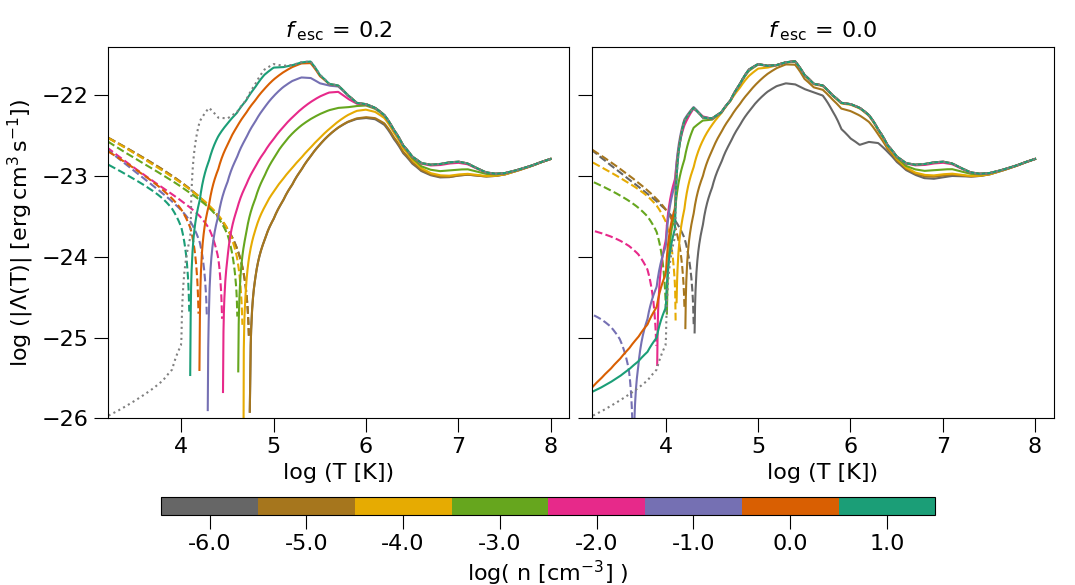
\includegraphics[width=1.0\textwidth]{plots/net_cooling.png}
    \caption{Net cooling function $\Lambda(n,T,r)$ as a function of the temperature $T$, for different values of the gas density $n$.
    %
    Note that the absolute value of $\Lambda$ is plotted: solid (dashed) lines represent positive (negative) values, i.e. net cooling (heating). 
    %
    The data for the cooling rates are taken from Gnedin \& Hollon \citep{gnedin2012cooling}, and we have used as input the values of the photoionization and photodissociation rates $\Gamma_{\mathrm{H}}$, $\Gamma_{\mathrm{He}}$, and $\Gamma_{\mathrm{LW}}$ derived in section  \ref{sec:radiation_fields}.
    %
    {\it Left}: case for $\fesc=0.2$, in which the ionizing radiation field is given by the sum of the flux from the galaxy ($\mathrm{SFR}=50\,\msun\mathrm{yr}^{-1}$) and the cosmic UVB at $z=6$. Results are shown at a galactocentric radius $r=1\,\mathrm{kpc}$. {\it Right}: case for $\fesc=0$. Ionizing radiation is only provided by the UVB. In both panels, The grey dotted line shows the cooling function under the hypothesis of Collisional Ionization Equilibrium (CIE; i.e., no radiation illuminating the gas).
    \label{fig:global_cooling}
    }
\end{figure*}

Having characterized the radiation fields that are present in the high-z galaxies' CGM, we can finally look at the thermal energy budget of the gas by focusing on the net cooling function $\Lambda(T)$. This is simply defined as the cooling function $\Lambda^\mathrm{(cool)}$ minus the heating function $\Lambda^\mathrm{(heat)}$, or, equivalently, as the total energy loss rate per unit volume ($\dot{\varepsilon}$) divided by the squared density ($\Lambda(T)=\dot{\varepsilon}/n^2$).

As already described, this function has a very complex dependence on many different physical variables, as all the atomic and molecular contributions to cooling and heating need to be taken into account. Even in the optically-thin case (and excluding the contribution of cosmic and X-rays), $\Lambda$ is a function of the temperature $T$, the gas density $n$, the fractional abundance $X_{ij}$ for the species $i$ (including atomic and ionic species, various molecules, and cosmic dust) at level $j$, and the mean specific intensity of the radiation field $J(\nu)$. 

A step forward in simplifying this function can be made by assuming that all the atoms and ions are in ionization equilibrium, i.e., the total (collisional + photoionization) rate of ionization is equal to the rate of recombination. Assuming that the levels are in equilibrium as well (excitation and de-excitation rates are identical), the net cooling function depends only on the gas temperature, density, and composition (metallicity), and, of course, on the radiation field strength $J(\nu)$. 

If no radiation is present, then equilibrium conditions are determined only by collisions: it is the so-called "\textit{Collisional Ionization Equilibrium}" (CIE) condition. Assuming CIE, we have seen that in the low-density limit the cooling rate (section \ref{sec:cooling}) does not depend on the density $n$, while the heating rate (sec. \ref{sec:heating}) is negligible as all the main heating processes rely on the energy carried by an incident radiation field. The only residual dependences, then, are temperature and metallicity; the grey dotted lines in figure \ref{fig:global_cooling} show the CIE cooling function for $Z=1\,Z_\odot$. 

As already mentioned, the presence of a UV radiation field acting on the gas affects the net cooling rate in two major ways: (a) it boosts the heating rate due to the photoelectric effect on gas and/or dust; (b) it alters the photoionization rates, reducing the abundances of cooling species such as \HI, \HeI, \CII and ultimately resulting in a lower emissivity of the gas. Overall, these effects tend to decrease significantly the value of $\Lambda$ at a given temperature, and they need to be carefully modeled to study the properties of the gas, especially in the low-density regime. 

In principle, the full spectral distribution of the specific intensity needs to be used in order to compute the abundance and the cooling/heating rates for every given species. However, this is very hard to do in practice, because it requires a lot of computational time. For this reason, in this work, we use the data tables created by Gnedin \& Hollon \citep{gnedin2012cooling} in order to determine the value of the net cooling function for the outflowing gas. 

The data tables are created by assuming low-density, optically thin gas in ionization equilibrium, and by neglecting the effects of cosmic and X-rays. Heating and cooling are computed using the \code{cloudy} spectral synthesis code \citep{ferland1994}, taking into input the temperature (T), density (n), and metallicity (Z) of the gas, as well as four other parameters that are meant to approximate well the complex dependence of $\Lambda$ on the incident radiation field. These parameters are: (1) the Lyman-Werner \HH photo-dissociation rate $\Gamma_\mathrm{H2}$; (2) the hydrogen photoionization rate $\Gamma_\mathrm{H}$; (3) the helium photoionization rate $\Gamma_\mathrm{He}$; (4) the \CVIion photoionization rate $\Gamma_\mathrm{CVI}$. They don't have any special meanings, but they are chosen because they can sample well the strength of the radiation field in all the regions of the spectrum, from the FUV one ($\Gamma_\mathrm{H2}$) to the EUV ranging from tens of eV ($\Gamma_\mathrm{H},\,\Gamma_\mathrm{He}$ to hundreds of eV ($\Gamma_\mathrm{CVI}$). 

We have already computed all these quantities for our physical environments in section \ref{sec:radiation_fields} (except for $\Gamma_\mathrm{CVI}$, which we set to a null value as it is important only for very hard radiation such as the one from quasars). Overall, three parameters determine the value of the total radiation fields (central galaxy + UVB): the galaxy's redshift ($z$), the star formation rate (SFR), and the escape fraction ($\fesc$); therefore, we can write the dependencies of the net cooling function as: $\Lambda = \Lambda(T,n,Z;r,\mathrm{SFR},z,\fesc)$. 

While the dependences on the SFR and on the redshift are sub-dominants, the escape fraction turns out to be a key factor governing the behaviour of the net cooling function. Given its uncertainty (section \ref{sec:first_lights_reionization}), we bracket all the possible values for the escape fraction by setting $\fesc = 0.2$ and $\fesc =0$. The former is consistent with the values used in most reionization studies \citep[e.g.,][]{Mitra15,Robertson15,Mitra18}, while the latter accounts for observations of very low $\fesc$ systems \citep[e.g.,][]{inoue2006escape,paardekooper2015first, ma2020no}. 

In figure \ref{fig:global_cooling}, we show the absolute value of the net cooling function, $|\Lambda(T)|$ for different values of the gas density (n), in the two extremal cases $\fesc=0.2$ (left panel) and $\fesc=0$ (right panel). The metallicity is taken to have a solar value ($Z=1\,Z_\odot$), while redshift and SFR are set to $z=6$ and $\mathrm{SFR}=50\,\msun\mathrm{yr}^{-1}$, respectively. For $\fesc=0.2$ the cooling function depends explicitly on the radius $r$: for displaying purposes, we fix $r=1\,\mathrm{kpc}$. In this case, as shown in section \ref{sec:radiation_fields}, the galaxy's radiation dominates over the UVB. For $\fesc=0$, instead, radiation from the galaxy is completely absorbed and the UVB is the only residual source of ionizing photons. 

Indeed, there are striking differences between the two $\fesc$ cases: in the left panel of figure \ref{fig:global_cooling} ($\fesc=0.2$), we see that the main effect of the strong galactic flux at a distance of $1$ kpc is to dramatically depress the ability of the gas to cool in the temperature range $10^{4-6}$ K, particularly for low gas densities. The decrease of the peaks is mostly produced by the fact that H (and partly also He) atoms, providing the main cooling channel via the excitation of the Ly$\alpha$ transition, become ionized and therefore unable to radiate efficiently. The equilibrium temperature, given by the condition $\Lambda=0$, is identified by the spikes in the curves, where a transition from cooling to heating-dominated regimes at lower $T$ takes place. The equilibrium values range in $\log T=4.1 - 4.7$, with the warmer solutions applying to lower densities. 

The situation is significantly different if ionizing radiation from the galaxy is not allowed to escape in the halo ($\fesc=0$, right panel). In this case, the much lower intensity of the UVB alone produces only a very limited suppression of the cooling function, and only for low densities, $n < 0.01\, \cc$. Equilibrium temperatures are consistently lower for $\fesc=0$, due to the smaller photoheating provided by the UVB. They range between $\log T=3.5 - 4.5$: this is consistent with the fact that the CGM/IGM of galaxies after reionization have temperatures around $10^4\,\mathrm{K}$, as they are not able to cool down any further due to the heating effect of the UVB. From this analysis, we conclude that the cooling function is heavily dependent on $\fesc$. As we will see, this has direct implications on the final emission of \CII in the model we are about to describe. 



 \section{Outflow model}\label{sec:outflow_model}



In this section, we can finally present our model in support of the \textit{outflow hypothesis} (sec. \ref{sec:theory_halos}). We focus on an instance of a normal star-forming, high-redshift galaxy, and we describe the properties of a galactic wind arising from the galaxy and expanding out into its CGM. Our aim is to derive physically-motivated density, velocity, and temperature radial profiles for the outflowing gas, and to use these quantities to compute the predicted \CII luminosity, in order to compare it with observations. 

We make use of the theoretical studies on SF-driven galactic outflows that we have introduced in section \ref{sec:model_outflows}. As a first exploratory investigation, we start by considering the CC85 model (sec. \ref{sec:cc85_model}). We summarize the crucial assumptions and results of the CC85 model in order to assess its validity and to look for possible improvements. The model considers the galaxy to be a sphere of radius $R$; hereafter, we take $R= 0.3\,\mathrm{kpc}$ as our fiducial value, as it is a good estimate for the average size of normal high-z galaxies \citep[e.g.,][]{Dayal:2018hft}. Energy and mass are injected inside the galaxy to model the effects of stationary SNe activity. The rates of energy ($\dot{E}$) and mass ($\dot{M}$) injection are:
\begin{subequations}
\begin{align}
    &\dot{E}=\alpha  E_{0,\mathrm{SN}} \nu_\mathrm{SN} \,\mathrm{SFR}\\
    & \dot{M}=\eta \, \mathrm{SFR},
\end{align}
\end{subequations}
where $E_{0,\mathrm{SN}} = 10^{51}\,\mathrm{erg}$ is the total energy released by a single SN, $\nu_\mathrm{SN}=10^{-2}\,\msun^{-1}$ is the rate of SNe per unit stellar mass, and SFR is the star formation rate. $\alpha$ and $\eta$ are the thermalization efficiency and the mass loading factor: these two parameters express the coupling between the wind and the ISM/SNe remnants in terms of energy and mass, respectively.
$\eta$ heavily affects the central gas density, and thus the general behavior of the system. Instead, the dependence of the physical variables on $\alpha$ is not as strong (especially considering radiative cooling effects, see e.g., eq. \ref{eq:eta_crit}), and to a first approximation, it can be fixed. For this reason, we have decided to set $\alpha=1$ (chosen accordingly to outflow observations by Strickland \& Heckman \citep{strickland2009supernova}), and retain $\eta$ as a free parameter. 

Eqs. \ref{eq:solinn} and \ref{eq:solout} express the solutions for the galactic wind arising in the CC85 setting for the inner and the outer regions, respectively. The solutions are expressed in terms of the Mach number $\mathcal{M}(r)=v(r)/c_s(r)$, where $c_s$ is the sound speed (eq. \ref{eq:sound_speed}), but can be recast in terms of physical quantities such as the velocity $v$, density $\rho$, and pressure $P$. A sketch for the radial profiles of these quantities can be found in figure \ref{fig:cc85} (note that in our discussion, we consider an adiabatic index $\gamma=5/3$). In figure \ref{fig:temp_CC85}, we show the same temperature profile for different values of the $\eta$ parameter, ranging from $0.2$ to $8.2$. We take a fiducial value for the star formation rate, $\mathrm{SFR}=50\,\msun\mathrm{yr}^{-1}$. For $r<R$ the temperature is roughly constant at $10^{7-8}\,\mathrm{K}$, with the exact value depending on $\eta$: more mass-loaded outflows are cooler. Beyond $R$, the temperature drops purely due to adiabatic cooling following the characteristic behavior $T\propto r^{-4/3}$. 

This drop in temperature is extremely important, as our goal is to create sufficient \CII emission in the gas, and this is possible only if the temperature gets lower than $T\lesssim10^4\,\mathrm{K}$. This is because carbon is collisionally ionized to \CIIIion (and higher ionization states) for temperatures above this threshold. Therefore, the presence of cool gas in the halo is essential to explain observations of \CII extended emission. Looking at figure \ref{fig:temp_CC85}, however, we realize that the adiabatic evolution assumed by the CC85 model results in a hot/warm outflow that has temperatures $T\gtrsim10^{4.5}\,\mathrm{K}$ (for all values of $\eta$) out to radial distances $r\gtrsim10\,\mathrm{kpc}$. Since the halos are observed in $10-15\,\mathrm{kpc}$ radii from the center, this implies that the CC85 model cannot account for the observed \CII emission. 

\subsection{Introducing cooling and gravity} \label{sec:cooling_gravity}



%

For this reason, motivated by the theoretical/observational studies of cool phases in outflows (section \ref{sec:outflows_cooling}), we abandon the adiabatic hypothesis by considering the possibility of gas heating and cooling. We have already described how a number of different works (in particular, Thompson et al. \citep{Thompson16}) have proved that, for high values of the mass loading factor $\eta$, energy losses are non-negligible in the CC85 model. We start from this point, and we aim at studying the transition between an adiabatic hot/warm mode in the outflow to a cool one due to the inclusion of radiative cooling.

We consider the same setting as the CC85 model: in particular, in the inner region ($r<R$), we retain the CC85's assumptions and thus recover the same solution eq. \ref{eq:solout} (for a discussion on this, see the end of section \ref{sec:outflows_cooling}). From this solution, we can express the physical conditions at the boundary region $r=R$ as (see also eqs. \ref{eq:bound_cc85_1}--\ref{eq:bound_cc85_3}):
\begin{subequations} \label{eq:boundary}
\begin{align}
&\rho(R)=\frac{\sqrt{2}}{4\pi}\,\frac{\dot{M}^{3/2}}{\dot{E}^{1/2}}\frac{1}{R^2}\propto {\rm SFR}\, \eta^{3/2}\\
&p(R)=\frac{3\sqrt{2}}{40\pi}\,\frac{\dot{M}^{1/2}\dot{E}^{1/2}}{R^2}\propto {\rm SFR} \,\eta^{1/2}\\
&v(R)=\frac{1}{\sqrt{2}}\,\frac{\dot{E}^{1/2}}{\dot{M}^{1/2}}\propto \eta^{-1/2}\,,\label{eq:v_boundary}
\end{align}
\end{subequations}
In the outer region, instead, we allow the gas to cool radiatively by introducing the net cooling function $\Lambda = \Lambda(T,n,Z;r,\mathrm{SFR},z,\fesc)$ in the hydrodynamical equations (eqs. \ref{eq:eul_cc85}). We obtain a new set of equations that can be integrated for $r>R$, using the physical relations at $r=R$ as boundary conditions for the system. 

\begin{figure}
	\centering
	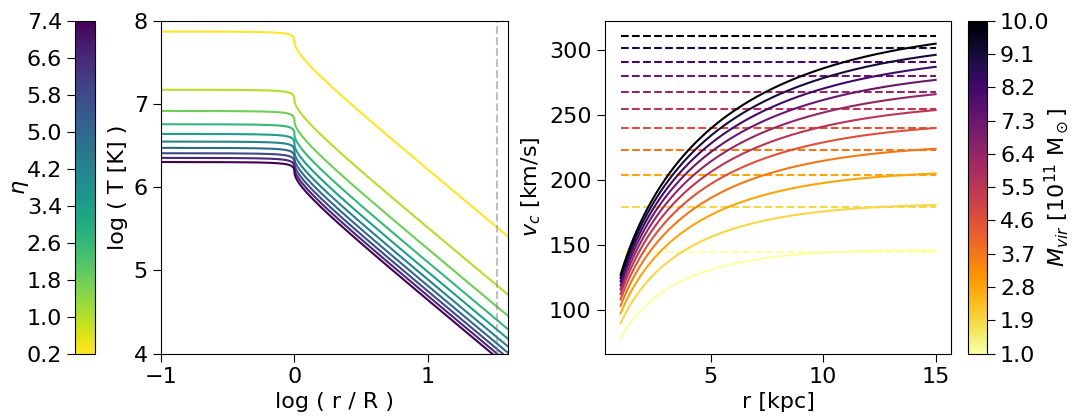
\includegraphics[width=1.0\textwidth]{plots/cc85+NFW.png}
	\caption{\textit{Left:} Outflow temperature (T) as a function of the radius (r) in the CC85 (adiabatic) model. The curves are calculated for $R=0.3\,\mathrm{kpc}$ and SFR$=50 \, \msun \rm yr^{-1}$. Different colors are used to map different values of the mass loading factor ($\eta$). \textit{Right}: local circular velocity as a function of the radius for a NFW \citep{NFW_profile} dark matter halo's density distribution. Different halos are color-coded according to their total virial mass. The dashed lines represent the maximum value reached by $v_c$, which is also the (constant) circular velocity profile it would result from an isothermal sphere distribution.
	\label{fig:temp_CC85}
	}
\end{figure}

However, we have yet to take another step forward. Since the outflow is slowed down because of energy losses, neglecting the dark matter halo's gravitational influence is not possible anymore. For this reason, we include a gravitational potential $\varphi(r)$ created by a dark matter distribution $\rho(r)$ in the Euler equation (eq. \ref{eq:eul2_cc85}). Exploiting the assumption spherical symmetry, as well as the Gauss theorem, we can write the radial gradient of the potential as:
\begin{align}
\frac{\d \varphi(r)}{\d r}=\frac{G M(r)}{r^2} = \frac{v_c^2(r)}{r}
\end{align}
In this expression, $M(r)$ is the total mass contained in a sphere of radius $r$, and $v_c(r)$ is the local circular velocity:
\begin{align}
v_{c}(r) &= \sqrt{\frac{GM(r)}{r}}
\label{eq:v_c_definition_model}
\end{align}
In principle, one should also include the gravitational contribution due to the baryonic component in the galaxy disk. However, we neglect this term, as the disk potential decreases faster than the DM halo potential as the galactocentric distance increases. This implies that beyond a kpc scale (where the physics of the outflow becomes more interesting) the disk contribution tends to be irrelevant, and dark matter dominates the gravitational energy budget.

As described in section \ref{sec:halos}, two main choices are possible for the dark matter halo's density profile. A simpler solution can be obtained by taking an isothermal sphere profile (eq. \ref{eq:iso_sphere}): in this case, $M(r)\propto r$, and then $v_c(r) = {\rm const}$. Therefore, with this choice, gravity can be implemented in a fairly straightforward way. However, such a profile builds up a lot of mass in the halo's core, resulting in a very strong slowing effect on the outflow, especially in the region where the outflow velocity is still relatively small. 

This motivates us to search for a different, more promising solution. With this respect, a more physically motivated candidate is the Navarro-Frenk-White (NFW) profile (eq. \ref{eq:nfw_profile}). This profile has a flatter core, and it mimics the observed/simulated profiles much more faithfully (sec. \ref{sec:halos}). The radial dependence of $v_c(r)$ -- or, equivalently, $M(r)$ -- is not as simple, but it still can be obtained analytically by integrating the density profile $\rho(r)$ in a volume of radius $r$:
\begin{align}
M(r) = \frac{M_{vir}}{A_\mathrm{NFW}}\, \left(\log\left(\frac{r_s + r}{r_s}\right) + \frac{r_s}{r_s + r} -1\right) 
\end{align}
where $M_{vir}$ is the virial mass of the halo, $A_\mathrm{NFW} = \log(1+c_N) - c_N/(1+c_N)$, and $r_s$ is the halo "scale radius", which is related to the virial radius via the \textit{concentration parameter} $c_N = r_{vir}/r_s$. Obviously, this formula holds valid only for $r<r_{vir}$. The virial radius can be determined from the virial mass by fixing a conventional overdensity $\delta_c = 200$, and knowing the average density ($\Bar{\rho}(z)$) of the universe at redshift $z$:
\begin{align}
r_{vir} = \left(\frac{3M_{vir}}{\Bar{\rho}(z)\,4\pi \delta_c}\right)^{1/3}
\end{align}
We obtain the concentration parameter (at a given virial mass and a given redshift) from the fit realized by Dutton \& Macciò \citep{dutton2014cold}. $M_{vir}$ and $z$ are therefore the only free parameters that need to be fixed in order to characterize completely the halo's gravitational potential $\varphi(r)$. For our convenience, we replace $M_{vir}$ with an equivalent parametrization, by introducing the global circular velocity $v_c = \sqrt{GM_{vir}/r_{vir}}$. 

Figure \ref{fig:temp_CC85} shows the radial NFW profiles for the local circular velocity $v_c(r)$, for different choices of the virial mass $M_{vir}$ -- or, equivalently, of the global circular velocity $v_c$. Note that, in the case of an isothermal sphere, the global and the local circular velocity are the same everywhere. Since $v_c$ is also the maximum value assumed by the local circular velocity $v(r)$, this implies that the effects of an isothermal sphere are much more dramatic than the ones of an NFW profile. Hereafter, we will consider the NFW prescription as the fiducial choice in our model.



\subsection{Physical profiles for the outflow} \label{sec:outflow_profiles}

Having specified the conditions for cooling and gravity, we can finally rewrite the hydrodynamical equations for the outflow in the region $r>R$: these are mass conservation, Euler equation, and energy conservation (eqs. \ref{eq:eul1_cc85}--\ref{eq:eul3_cc85} with $q=Q=0$). Euler equation changes because of the presence of a gravitational force due to the dark matter halo's potential. The energy conservation equation, on the other hand, needs to take into account the energy losses due to radiative cooling. It is convenient to write the energy balance making use of the first principle of thermodynamics:
\begin{align}
-\d \varepsilon = \d u - \frac{P}{n}\,\d n,
\end{align}
where $\d \varepsilon$ is the total energy lost (note the minus sign) by the system, and $\d u$ is the change in the internal energy; both quantities are defined per unit volume. Exploiting this relation, we can write the energy balance for the spherical flow as:
\begin{align}
-\dot{\varepsilon}  = uv \,\frac{1}{T}\frac{\d T}{\d r} - Pv\,\frac{1}{n}\frac{\d n}{\d r} = - n^2 \,\Lambda,
\end{align}
where we have used the definition of the net cooling function $\Lambda = \Lambda^\mathrm{(cool)}-\Lambda^\mathrm{(heat)}$. 

Given these premises, we can write the set of equations describing the outflow as: 
\begin{subequations}
\begin{align}
&\frac{1}{r^2}\der{}{r}(r^2v\rho) =0, \label{eq:neweul1}\\
&\rho v\der{v}{r} = -\der{p}{r} - \rho \der{\varphi}{r} \label{eq:neweul2}\\
&\left(\frac{1}{T}\der{T}{r} - (\gamma-1)\frac{1}{\rho}\der{\rho}{r}\right) v k_B T = - (\gamma-1) n \Lambda \label{eq:neweul3}
\end{align}
\end{subequations}
Combining these three equations we get a first order system of ODE that can be integrated numerically to solve for the variables $\rho$, $v$, and $T$. It is convenient to express these equations in terms of the flow Mach number $\mathcal{M}=v/c_s$, the gravitational Mach number $\mathcal{M}_g=v_c/c_s$, and the cooling time $\tau_\Lambda =  k_B T/n\Lambda$ (eq. \ref{eq:tcool}):
\begin{subequations}
\begin{align}
&\der{\log\rho}{\log r}=2 \left(\frac{\mathcal{M}^2-\mathcal{M}_g^2/2}{1-\mathcal{M}^2}\right)- \frac{r}{\lambda_\Lambda}\left(\frac{1}{1-\mathcal{M}^2}\right) \label{eq:cooling_model_equations_n}\\
&\der{\log v}{\log r}=\left(\frac{\mathcal{M}_g^2-2}{1-\mathcal{M}^2}\right)+\frac{r}{\lambda_\Lambda}\left(\frac{1}{1-\mathcal{M}^2}\right) \label{eq:cooling_model_equations_v}\\
&\der{\log T}{\log r}={2(\gamma-1)}\left(\frac{\mathcal{M}^2-\mathcal{M}_g^2/2}{1-\mathcal{M}^2}\right)-\frac{r}{\lambda_\Lambda}\left(\frac{1-\gamma\mathcal{M}^2}{1-\mathcal{M}^2}\right)\,, \label{eq:cooling_model_equations_T}
\end{align}
\label{eq:cooling_model_equations}
\end{subequations}
where $\lambda_\Lambda=(\gamma/(\gamma-1)) v \tau$ is the cooling length.

The cooling function $\Lambda$ (and, in turn, the cooling length $\lambda_\Lambda$) depends on a number of parameters that needs to be fixed to solve the system of equations for the outflow: the metallicity ($Z$), the redshift ($z$), the star formation rate (SFR), and the escape fraction ($\fesc$). The gravitational potential adds a further dependence on the global circular velocity ($v_c$) of the halo. In what follows, we set some values for these parameters, in order to solve the equations in some cases of interest and discuss the resulting solutions for the outflows. We will investigate further other choices for the parameters in section \ref{sec:CII_emission}. 

First of all, we consider solar metallicity for the outflow ($Z=1\,Z_\odot$); this is equivalent to say that the ISM of high redshift galaxies has metallicities equal to (or close to) solar values. This statement is supported by simulations of high-z galaxies \citep[e.g.,][]{pallottini2017} and by the extrapolation of the local mass-metallicity relation to higher redshifts \citep[e.g.,][]{mannucci:2012}. Redshift, star formation rate, and circular velocity can be gauged with sufficient accuracy from observations. For this reason, we will set their values guided by observations in the next chapter. Here, we employ some fiducial values that are reasonable for normal, star-forming, high-z galaxies: $z=6$, $\mathrm{SFR}=50\,\msun\mathrm{yr}^{-1}$, $v_c = 200\,\kms$. Since $\fesc$ can change dramatically the energy balance of the gas, we study here the same two configurations $\fesc=0.2$ and $\fesc =0$ that we have considered in section \ref{sec:cooling_function}.


Figure \ref{fig:global_profiles} shows the radial profiles of the key hydrodynamical variables, $v, n, T$ for different values of the mass load parameter, $\eta$. In the left panel, we set $\fesc=0.2$, while in the right panel consider only the UVB radiation by setting $\fesc=0$. The first thing to note is that both velocity and density are not strongly affected by the choice of different values for the escape fraction $\fesc$. Therefore, we can conclude that a different prescription for the radiation impinging on the gas has only a secondary effect on its density and velocity. 

In both columns, for low values of $\eta$ ($\eta \lesssim 1$), the radial asymptotic dependencies are the same as the CC85 model: $v \approx \mathrm{const.}$ and $n\propto r^{-2}$. This implies that cooling, for these low-$\eta$ values, is not efficient enough, and thus the evolution is approximately adiabatic in the whole range of radii considered. This is supported by the temperature profiles of these outflow modes -- which resembles a power-law in all $\fesc$ scenarios -- and it is perfectly in line with the analytical estimates we have outlined in section \ref{sec:outflows_cooling}. 

When $\eta$ increases to values higher than unity, instead, cooling starts to become efficient, and the evolution changes considerably. The initial density becomes high enough for gravity to become important. This reduces the velocity up to a stalling radius, $r_{\rm stop}$, where the velocity drops to zero. The position of the stalling point moves closer to the galaxy as $\eta$ increases. Because of the gas slowing down, the density tends to increase in the outer regions of the outflow, becoming greater and greater as the distance approaches the stalling radius $r_\mathrm{stop}$. 

We note that the presence of a stalling radius is a consequence of our assumptions of stationarity and spherical symmetry. In a time-dependent scenario, the gas, after being halted by the gravitational potential of the halo, would fall back forming a galactic fountain and mixing with the outflow. Our semi-analytic study cannot capture the complexity of this process. However, we believe that studying for which conditions gravity can halt the gas and thus increase its density in the outer layers of the outflow is already an important step towards a full comprehension of this complex phenomenon.

Cooling introduces new, striking features in the temperature profiles shown in the lower panels of figure \ref{fig:global_profiles}. For high values of the mass loading factor ($\eta \gtrsim 1$) the gas starts cooling at a distance $r_{\mathrm{cool}}$ that gets smaller as $\eta$ increases. The cooling is quite rapid, supporting the "catastrophic cooling" scenario already studied by several previous works (see section \ref{sec:outflows_cooling}). After cooling has taken place, the gas temperature evolution depends on our choice for $\fesc$. If we include the radiation from the galaxy (i.e., $\fesc=0.2$), cooling stops at an equilibrium temperature of around $10^4 \,\mathrm{K}$. Beyond the cooling radius, the outflow is subject to a quasi-isothermal expansion. For $\fesc=0$, the temperature profiles are quite different, as expected from the different behaviors of the cooling function (figure \ref{fig:global_cooling}). The gas is able to cool down further to a temperature of a few hundred degrees. At larger radii, however, the gas slowly heats up, as the net cooling function takes negative values (i.e. the photoionization heating takes over as density decreases). As we will show in the next few paragraphs, temperatures of a few $\times 100$K allow a significant presence of \CIIion, and thus a potentially observable \CII emission. 




\begin{figure*}
    \centering
    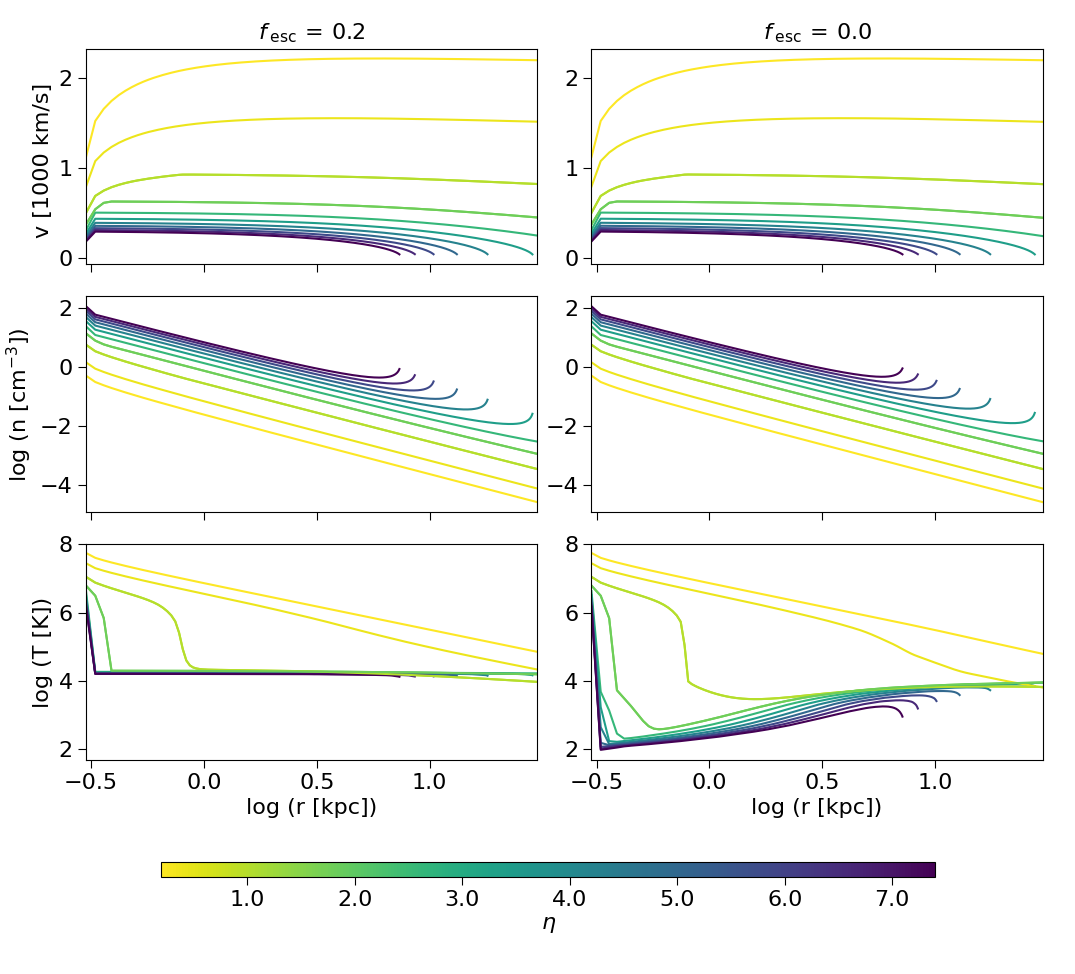
\includegraphics[width=1.\textwidth]{plots/profiles.png}
    \caption{Radial profiles of key outflow thermodynamical variables obtained for our model including cooling and gravity (eqs. \ref{eq:cooling_model_equations}). Shown are the two cases $\fesc=0.2$ (left column), and $\fesc=0$ (right).
    \textit{Top row}: Velocity ($v$). For high values of the mass loading factor $\eta$, gravity slows down the outflow until a stalling radius at which $v=0$ is reached.
    %
    \textit{Middle}: Density ($n$). The radial dependence of the density is generally $n\propto r^{-2}$, but its value increases as the gas slows down due to gravity.
    %
    \textit{Bottom}: Temperature ($T$). Note the different temperature profiles beyond the cooling radius. For $\fesc=0$ the outflow cools to lower temperatures and reaches the equilibrium value of $T\approx10^4\,\mathrm{K}$ only at much larger radii.  
    \label{fig:global_profiles}
    }
\end{figure*}

\begin{comment}

\subsection{Some analytical considerations} \label{sec:analytical}

WRITE ABOUT ANALYTICAL APPROACH ETC

MENTION THE SHARP DEPENDENCE OF V ON ETA

The dependence of the stalling radius, $r_\mathrm{stop}$, on the SFR can be inferred from eq. \ref{eq:cooling_model_equations_v}. For temperatures $T\approx10^{2-4}\, \mathrm{K}$, the flow is highly supersonic. Also, the cooling length of the gas remains larger than the outflow extent. Hence, using these approximations it is straightforward to obtain an analytical solution for the profile $v(r)$ (see also \citet{Thompson16}), from which it follows that
\begin{align}
r_\mathrm{stop} \approx r_\mathrm{cool}\,e^{v^2(r_\mathrm{cool})/2v_c^2},
\end{align}
which implies that $r_\mathrm{stop}$ increases with the cooling radius, $r_\mathrm{cool}$. As the latter has a strong inverse dependence on the outflow rate $\eta {\rm SFR}$ \citep{Thompson16}, a higher SFR value results in a smaller $r_\mathrm{stop}$. Hence, beyond $r_\mathrm{stop}$ the emission drops to zero. 
%
\end{comment}

\subsection{Ionization state of the gas}\label{sec:ionization_structure}


Knowing the density and temperature of the outflowing gas, we can compute the ionization state of different species as a function of the radial distance from the galaxy. This is an important step towards the computation of the final \CII emission, as the energy emitted by the \CII transition depends on the numerical abundances of free electrons and singly ionized carbon (eq. \ref{eq:CII_cooling}).

We start by assuming that the free electron density is equal to the \HI density, i.e., $n_e \approx n_p$. This means that we neglect contributions from other ionized species, such as He and C, because of their lower abundance and/or higher (for He) ionization potential. Then, assuming ionization equilibrium, we write the statistical balance for hydrogen ionization by equating the rates of photoionization ($\Gamma_{\mathrm{H}}$) and collisional ionization ($k_{\mathrm{H}}$) with the recombination rate ($\eta_{\mathrm{H}}$):
\begin{align}
n_\mathrm{H} \Gamma_{\mathrm{H}} + n_\mathrm{H} n_e k_{\mathrm{H}} = n_e\, n_{p} \,\eta_{\mathrm{H}}
\label{eq:ion_bal}
\end{align}
We have already computed the value of $\Gamma_\mathrm{H}$ in section \ref{sec:radiation_fields}. For $\eta_H$, we use the power-law approximation to Case B radiative recombination given by \citet{tielens2005book},
\begin{align}
\eta_\mathrm{H} = 4.18 \times 10^{-13} \, \bigg(\frac{T}{10^4 \, \mathrm{K}}\bigg)^{-0.75} \,\, \mathrm{cm}^3\, \mathrm{s}^{-1}
\label{eq:beta_H}
\end{align}
$k_\mathrm{H}$ is taken from \citet[][Appendix B]{bovino:2016aa}.

Using $n_\mathrm{p} + n_\mathrm{H} = \mathcal{A}_\mathrm{H} n$, where $A_\mathrm{H}$ is the cosmic hydrogen abundance ($A_{\mathrm{H}} = 0.76$ for solar composition \citep{asplund2009}), $n$ is the total gas density, and defining $x_\mathrm{e}=n_\mathrm{e}/n$, we can recast eq. \ref{eq:ion_bal} in the following form:
\begin{align}
(\eta_\mathrm{H}+k_\mathrm{H})\,x_e^2 + \bigg(\frac{\Gamma_{\mathrm{H}}}{\mathcal{A}_H n}-k_\mathrm{H}\bigg)\,x_e - \frac{\Gamma_\mathrm{H}}{\mathcal{A}_H n}= 0
\label{eq:ne}
\end{align}
Solving this quadratic equation, the H ionization fraction $x_e$ can be obtained. 
 
We now turn to carbon, and write the equivalent ionization equations assuming a detailed balance among three states of C atoms ionization: neutral (with number density $n_{\mathrm{CI}}$), singly ionized ($n_{\mathrm{CII}}$), and doubly ionized ($n_{\mathrm{CIII}}$).
\begin{subequations}
\begin{align}
n_\mathrm{CI} \Gamma_{\mathrm{CI}} + n_\mathrm{CI} n_e k_{\mathrm{CI}} &=n_e\, n_\mathrm{CII} \,\eta_{\mathrm{CII}}\\
n_\mathrm{CII} \Gamma_{\mathrm{CII}} + n_\mathrm{CII} n_e k_{\mathrm{CII}}&=n_e\, n_\mathrm{CIII} \,\eta_{\mathrm{CIII}}
\end{align}
\end{subequations}
The photoionization, collisional ionization, and recombination coefficients are $\Gamma_{\mathrm{CI}}$, $\Gamma_{\mathrm{CII}}$, $k_\mathrm{CI}$, $k_\mathrm{CII}$, and $\eta_{\mathrm{CII}}$, $\eta_{\mathrm{CIII}}$, respectively. Again, we can write the constraint $n_\mathrm{CI}+n_\mathrm{CII}+n_\mathrm{CIII}=\mathcal{A}_\mathrm{C} n \equiv n_\mathrm{C}$, with the carbon abundance taken to be equal to the Solar value $\mathrm{A}_{\mathrm{C}} = 2.69 \times 10^{-4}$ \citep{asplund2009}. Using this relation, we can solve the equations above and obtain the ionization fraction of carbon $x_\mathrm{CII}= n_\mathrm{CII}/n_\mathrm{C})$:
\begin{align}
x_\mathrm{CII} = \bigg(1+\frac{\Gamma_{\mathrm{CII}}}{n_e\,\eta_{\mathrm{CIII}}}+\frac{n_e\,\eta_{\mathrm{CII}}}{\Gamma_{\mathrm{CI}}+n_e k_\mathrm{CI}}+ \frac{k_\mathrm{CII}}{\eta_\mathrm{CIII}}\bigg)^{-1} \label{eq:densityCII}
\end{align}

The photoionization rates $\Gamma_{\mathrm{CI}}$ and $\Gamma_{\mathrm{CII}}$ have also been computed in section \ref{sec:radiation_fields} (eqs. \ref{eq:ionization_states_gal}--\ref{eq:ionization_states_uvb}) taking into account both the galaxy and the UVB contributions. Recombination rates must include both radiative and dielectronic recombination. For these, we use the following approximations \citep{tielens2005book}: 
\begin{subequations}
\begin{align}
\eta_\mathrm{CII} &= 10^{-13} \bigg[ 4.66 \bigg(\frac{T}{10^4 \, \mathrm{K}}\bigg)^{-0.62} + 1.84  \bigg]\,\, \mathrm{cm}^3\, \mathrm{s}^{-1}\\
\eta_\mathrm{CIII} &=10^{-12} \bigg[ 2.45  \, \bigg(\frac{T}{10^4 \, \mathrm{K}}\bigg)^{-0.65} + 6.06 \bigg]\,\, \mathrm{cm}^3\, \mathrm{s}^{-1}
\end{align}
\end{subequations}
%
Finally, we take the collisional ionization rates, $k_\mathrm{CI}$ and $k_\mathrm{CII}$, from \citet[][Table 1]{voronov_practical_1997}.


The resulting ionization radial profiles are shown in figure \ref{fig:global_ionization}. Again, there are dramatic differences between the two cases $\fesc=0.2$ and $\fesc=0$. If $\fesc=0.2$, the ionization radiation coming from the galaxy has dramatic effects on the gas: both H and C atoms are strongly photoionized by this radiation, and they are largely found in the form of \HII and \CIIIion. In particular, the fraction of singly ionized carbon is $x_{\rm CII}=n_{\rm CII}/n_C \lesssim 10^{-3}$. Such a small abundance of \CIIIion is problematic, because it suppresses the \CII emission and thus it is not compatible with the observations of \CII halos that we aim to explain. 

The $\fesc=0$ case, on the other hand, gives results that are much more promising. In the right panels of figure \ref{fig:global_ionization}, we see that models that undergo catastrophic cooling can produce considerable amounts of \CIIion. As the gas cools to a few hundred degrees K beyond $r_{\rm cool}$, carbon recombines, and $x_{\rm CII} \gsim 0.5$ in most cases but the lowest values of $\eta$. The outflow is essentially neutral as H has also largely recombined. As the outflow temperature increases again towards larger radii, because of the UVB photoheating, \CIIion ions are collisionally (and photo-) ionized, and their abundance decreases, albeit remaining significant. 

Therefore, our model seems to hint at the fact that only very low values of the escape fraction $\fesc$ are compatible with an appreciable presence of \CII in the outflow. This implies that the outflow hypothesis may be compatible with observations only if dust and/or \HI absorption prevents the galaxy's radiation from ionizing the \CIIion in the wind. For this reason, in the following analysis, we will concentrate on the case $\fesc=0$, which is the only one to be compatible with observations. The behavior of the gas ionization state in the outflow raises the interesting possibility that outflows might be used to indirectly probe the escape fraction $\fesc$. We will return to this point later on.


\begin{figure*}[t]
    \centering
    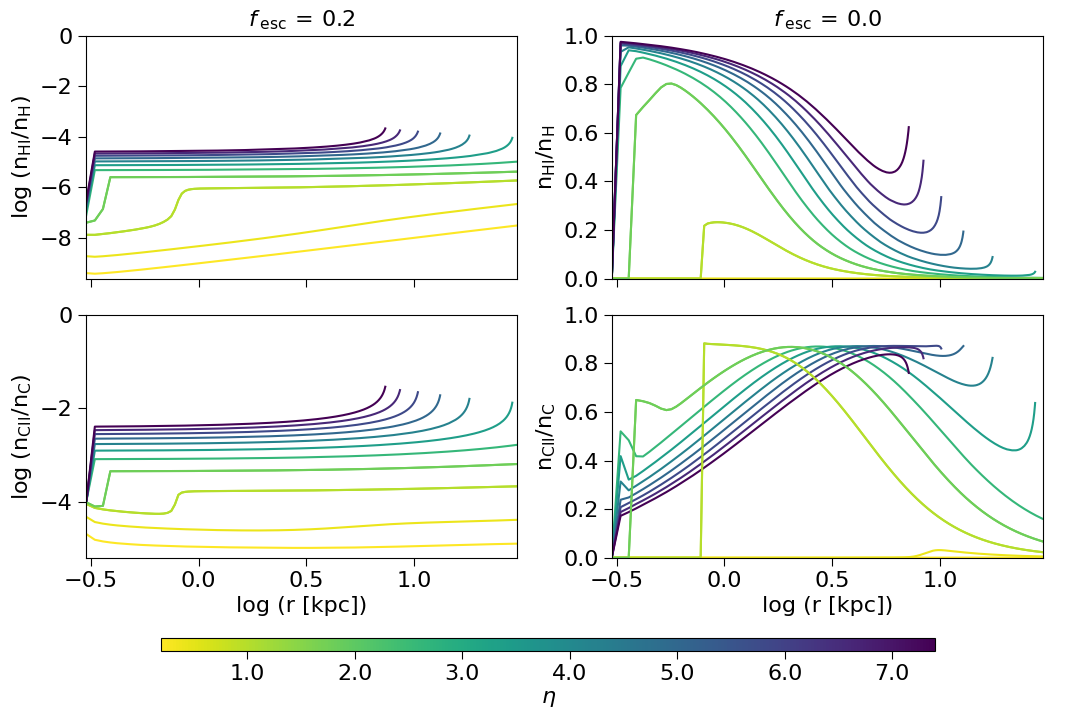
\includegraphics[width=1.0\textwidth]{plots/ions.png}
    \caption{Outflow radial ionization profiles. Shown are the two cases $\fesc=0.2$ (left column), and $\fesc=0$ (right). Note the linear scale in the right panels.
    %
    \textit{Top row}: Neutral hydrogen fraction (eq. \ref{eq:ne}). \textit{Bottom}: Singly ionized carbon fraction from eq. \ref{eq:densityCII}.
    \label{fig:global_ionization}
    %
    }
\end{figure*}


\section{[CII] line emission}\label{sec:CII_emission}


The emissivity of the \CII line $\dot{\varepsilon}_\mathrm{CII} = n^2 \Lambda^\mathrm{(cool)}_\mathrm{CII}$ can simply be determined using eq. \ref{eq:CII_cooling}. It is a function of the gas temperature $T$, of the free electron density $n_e$, and of the \CIIion density $n_\mathrm{CII}$. Using the ionization fractions computed at the end of last section, these densities can be expressed as a function of the gas density $n$:
\begin{subequations}
\begin{align}
&n_e = x_e(r)\,\mathcal{A}_\mathrm{H}\,n(r)
&n_\mathrm{CII} = x_\mathrm{CII}(r)\,\mathcal{A}_\mathrm{C}\,n(r)
\end{align}
\end{subequations}
Then, the final expression for the emissivity as a function of the radius $r$ is:
\begin{align}
 \dot{\varepsilon}_\mathrm{CII} (r) = 8.2\times10^{-21} \,\left(\frac{92\,\mathrm{K}}{T(r)}\right)^{1/2}\,n^2(r)\,\mathcal{A}_\mathrm{H}\,\mathcal{A}_\mathrm{C}\,x_e(r) \,x_\mathrm{CII}(r) \,e^{-92\ \mathrm{K}/kT(r)}\,\,\mathrm{erg}\,\mathrm{s}^{-1}\mathrm{cm}^{-3} \label{eq:emissivity_CII}
\end{align}
From the emissivity, the \CII surface density ($\Sigma_\mathrm{CII}$) can be obtained. The computation of $\Sigma_\mathrm{CII}$ is simplified by noting that, in most cases, the \CII emission is optically thin \citep[e.g.,][]{osterbrock1992}. Then, the \CII surface density at a point $(x,y)$ in the image plane is simply obtained by integrating the emissivity along the line of sight (parametrized by $h$:
\begin{align}
\Sigma_\mathrm{CII}(x,y)=\int\dot{\varepsilon}_\mathrm{CII}(s)\,\d s
\label{eq:emissivity}
\end{align}
Exploiting the symmetry of our model, we can express $\Sigma_\mathrm{CII}$ as a function of a single variable, the impact parameter $b$ (i.e., the distance between the line of sight and the center of the galaxy). Eq. \ref{eq:emissivity} can then be written as:
\begin{align}
\Sigma_\mathrm{CII}(b)&=\int_{-\infty}^{+\infty} \dot{\varepsilon}_\mathrm{CII}(r(s))\, \d s = 2 \int_{b}^{+\infty} \dot{\varepsilon}_\mathrm{CII}(r)\, \frac{r}{\sqrt{r^2 - b^2}}\,\d r \,
\label{eq:final_intensity}
\end{align}
Obviously, this final \CII surface density depends implicitly on a much greater number of parameters, such as mass loading factor, metallicity, redshift, SFR, circular velocity, and escape fraction. This dependence is hidden inside the thermodynamical variables and the ionization states in the outflow.  If all these parameters are set, then we have a prescription to compute the expected \CII emission, and we can compare this quantity with observations. However, in this discussion, we have neglected an important effect that may have a relevant effect on our final \CII emission. This effect is caused by the interaction of CMB photons with \CIIion atoms, and it is the subject of the next paragraph. 

\subsection{Correcting for the CMB suppression}\label{sec:CMB_suppression}


\begin{figure*}
    \centering
    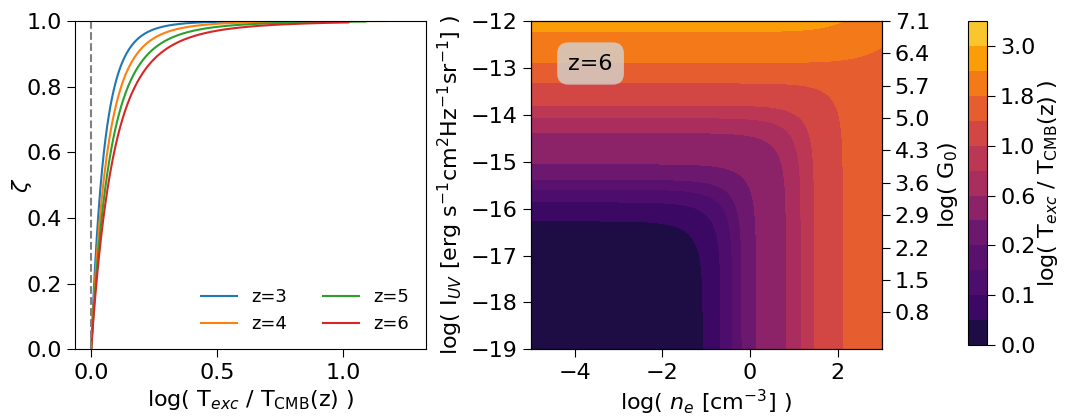
\includegraphics[width=1.\textwidth]{plots/cmb_theory.png}


    \caption{\textit{Left}: CMB suppression factor $\zeta$ (eq. \ref{eq:suppression_factor}) as a function of the ratio between $T_\mathrm{exc}$ and $T_\mathrm{CMB}(z)$, for different values of the redshift $z$. \textit{Right}: color map showing the ratio between the excitation temperature and the CMB one ($T_\mathrm{exc}/T_\mathrm{CMB}(z)$), computed at redshift $z=6$, as a function of the free electrons density $n_e$ and the UV intensity $I_{UV}$ at $1330$ \AA.
    \label{fig:cmb_intro}
    }
\end{figure*}


At high redshifts, new physical mechanisms become important, and they have to be taken into account by theoretical models. The CMB suppression is an instance of these effects that characterize the high redshift universe. As we have described in section \ref{sec:intro_cosmo}, the Cosmic Microwave Background is relic radiation that pervades the whole universe from the time of last-scattering. CMB photons follow a black body distribution  (eq. \ref{eq:black_body}) with an average temperature that scales with redshift as $T_\mathrm{CMB}(z) = T^{(0)}_\mathrm{CMB} (1+z)$ ($T^{(0)}_\mathrm{CMB}=2.73\,\mathrm{K}$ is the temperature of the CMB we measure today). Therefore, as redshift increases, CMB photons are more energetic, and they start to have a non-negligible effect on atomic transitions, particularly in the FIR/radio region of the spectrum. 

This effect is twofold: on one side, the presence of pervading radiation acting on the gas affects the level populations, and hence the \CII transition rate; on the other, any \CII emissions will be observed against a uniform CMB background, and this needs to be taken into account when computing the \CII surface density. 

The CMB radiation alters the level balance equation (eq. \ref{eq:level_eq}) by providing an absorption and a stimulated emission rates:
\begin{equation}
    n_l \,n_e\,\gamma_{lu} + n_l \,B_{lu}\, I(\nu_*) = n_u\,n_e\,\gamma_{ul} + n_u\,A_{ul} + n_u\, B_{ul} \,I(\nu_*)
\end{equation}
In this equation, we are considering the two-level system created by the \CIIion fine structure doublet, $^2P_{3/2}-\,^2P_{1/2}$; the transition associated with this system has a frequency $\nu_* = 1900\,\mathrm{GHz}$. $n_l$ and $n_u$ are the numeric densities of the two levels, and $n_e$ is the density of free electrons (the main collisional partners for \CII, see sec. \ref{sec:cooling}). $I(\nu) = B(\nu, z)$ is the (black-body) specific intensity of the CMB radiation. The Einstein coefficients and collisional rates have already been defined in section \ref{sec:cooling} and can be found in \citet{gong2012}. This balance equation is correct for a pure two-level system. However, \CII contains many other levels, and transition with more energetic levels is possible if the radiation illuminating the gas is energetic enough. In particular, in the presence of FUV radiation at $1330$ \AA, electrons can be pumped from the $^2P_{3/2}$ ($^2P_{1/2}$) level to $^2D_{3/2}$ at $1335.66$ \AA ($1334.53$ \AA). Then, this pumping effect can lead to the CII fine structure transitions $^2D_{3/2}\rightarrow \,^2 P_{3/2} \rightarrow \,^2 P_{1/2}$, resulting in a mixing of the levels we are interested in. Since we are including FUV radiation from the UV background and the parent galaxy, we need to include the UV excitation and de-excitation rates in the balance equation, to account for this \textit{UV-pumping} effect \citep[for more details, see][]{gong2012, vallini2015, kohandel:2019}. These rates are given by the following expressions \citep{field}:
\begin{align}
    P_{ul}^\mathrm{(UV)} &= \frac{g_k}{g_u}\frac{A_{kl}A_{ku}}{A_{kl}+A_{ku}}\left(\frac{c^2 I_\mathrm{UV}(\nu_{ku})}{2h\nu_{ku}^3}\right)&
    P_{lu}^\mathrm{(UV)} &= \frac{g_k}{g_l}\frac{A_{kl}A_{ku}}{A_{kl}+A_{ku}}\left(\frac{c^2 I\mathrm{UV}(\nu_{kl})}{2h\nu_{kl}^3}\right)
\end{align}
where “$k$” stands for the level $^2D_{3/2}$ ($g_k = 4$ is the level degeneracy), and $I_\mathrm{UV}$ is the UV radiation intensity. $A_{kl} = 2.41\times10^8\,\mathrm{s}^{-1}$ ($\nu_{kl}$) and $A_{ku} = 4.76\times 10^7\,\mathrm{s}^{-1}$ ($\nu_{ku}$) are the Einstein
coefficients (frequencies) of the $^2D_{3/2}\rightarrow \,^2P_{1/2}$ and $^2D_{3/2} \rightarrow \,^2P_{3/2}$ transitions, respectively.  

Accounting for the UV-pumping effect, yields:
\begin{equation}
    n_l \,n_e\,\gamma_{lu} + n_l \,B_{lu}\, I(\nu) + P_{lu}^\mathrm{(UV)} = n_u\,n_e\,\gamma_{ul} + n_u\,A_{ul} + n_u\, B_{ul} \,I(\nu) + P_{ul}^\mathrm{(UV)}
\end{equation}
This equation can be rewritten by introducing the excitation temperature $T_\mathrm{exc}$, in the same exact way as eq. \ref{eq:t_exc}. Using the relations linking the three Einstein coefficients (eqs. \ref{eq:einstein_coeff}), and the two collisional rates (eq. \ref{eq:coll_rates}), we obtain the following expression for $T_\mathrm{exc}$ ($T_*\approx 91\,\mathrm{K}$ is the transition temperature):
\begin{equation}
    \frac{T_*}{T_\mathrm{exc}} = \log\left( \frac{A_{ul}\left(1+c^2I(\nu_*)/2h\nu_*^3\right))+n_e\gamma_{ul}+P_{ul}^\mathrm{(UV)}}{A_{ul}\,c^2I(\nu_*)/2h\nu_*^3+n_e\gamma_{ul}\,e^{-T_*/T}+P_{lu}^\mathrm{(UV)}} \right)
\end{equation}
We can study this expression in different configurations: for high $n_e$ densities, collisions dominate and the excitation temperature tends to the gas kinetic temperature $T$; in the same way, if a strong UV flux is illuminating the gas, the excitation temperature gets approximately equals to the UV color temperature ($T_\mathrm{UV}\approx 10^4\,\mathrm{K}$), defined as $T_\mathrm{UV} = T_*\log\left(g_u P_{ul}^\mathrm{(UV)}/g_l P_{lu}^\mathrm{(UV)}\right)$. For low $n_e$ densities and weak UV fluxes, the excitation temperature gets closer and closer to the CMB temperature $T_\mathrm{CMB}(z)$: in this case, the \CII emission is strongly suppressed, because it becomes indistinguishable from the CMB background. Figure \ref{fig:cmb_intro} shows these different possibilities for $z=6$.

Using the excitation temperature, a straightforward radiative transfer calculation gives the ratio $\zeta$ between the specific intensity of the radiation observed against the CMB and the intrinsic one \citep[see e.g.,][]{dacunha2013}: 
\begin{equation}
    \zeta = 1-\frac{B_{\nu_*}(T_\mathrm{CMB}(z))}{B_{\nu_*}(T_\mathrm{exc})},
    \label{eq:suppression_factor}
\end{equation}
where $B_\nu$ stands for the black body distribution (eq. \ref{eq:black_body}). The left panel of figure \ref{fig:cmb_intro} shows the value of $\zeta$ as a function of the ratio between $T_\mathrm{exc}$ and $T_\mathrm{CMB}(z)$, for different values of the redshift $z$.

In order to account for the CMB effects on the \CII emission in our model, we compute the suppression factor $\zeta(r)$ in the wind, taking as inputs the redshift, the radiation fields, and the thermodynamic/ionization state of the gas. Then, we add this factor to the integral defining the \CII surface density; we obtain:
\begin{align}
\Sigma_\mathrm{CII}(b)=2 \int_{b}^{+\infty}\zeta(r) \,\dot{\varepsilon}_\mathrm{CII}(r)\, \frac{r}{\sqrt{r^2 - b^2}}\,\d r \,
\label{eq:cmb_final_intensity}
\end{align}
Figure \ref{fig:global_emission_cmb} shows the value of the parameter $\zeta$ in the wind (left panel) and the value of the \CII surface density obtained by taking into account the CMB suppression (right). The effects of CMB suppression are highlighted by showing (in semi-transparent colors) the emission profiles that would have been obtained for $\zeta =1$ (no suppression). The final $\Sigma_\mathrm{CII}$ profiles are obtained using eq. \ref{eq:cmb_final_intensity}, taking as input the thermodynamic and ionization state of the outflow (figures \ref{fig:global_profiles}--\ref{fig:global_ionization}). Note that all the parameters except for the mass loading factor $\eta$ are fixed to their fiducial values discussed in section \ref{sec:outflow_profiles}). We conclude that the CMB effect on the final \CII emission is significant, with depletion factors in the range $\zeta \approx0.2-0.7$.



\begin{figure*}
    \centering
    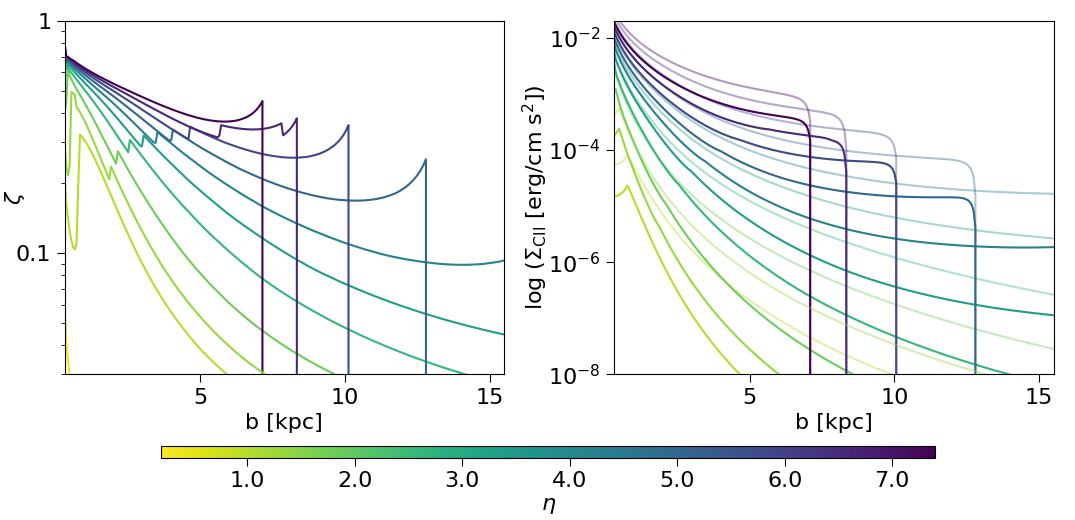
\includegraphics[width=1.0\textwidth]{plots/cmb_emission.png}
    \caption{\textit{Left}: suppression factor $\zeta$ as a function of the impact parameter $b$, for different values of the mass loading factor $\eta$. \textit{Right}: \CII surface density $\Sigma_\mathrm{CII}$, computed for $\zeta(r)$ showed in the left panel, as well as for $\zeta =1$ (transparent lines).
    \label{fig:global_emission_cmb}
    }
\end{figure*}





\subsection{Computing the final emission profiles}


In the last paragraphs, we have successfully computed the \CII surface density for our outflow model. Our final aim is to compare the results of our model with the observations of extended \CII emission reported in chapter \ref{chap:halos}. In order to do that, however, we need to convert the surface density into a flux per unit solid angle (or surface brightness), which is the quantity that is actually measured by observers (e.g., figure \ref{fig:fuji_data}). We do this by dividing $\Sigma_\mathrm{CII}$ by the observed \CII linewidth $\Delta\nu_\mathrm{obs}$:
\begin{align}
\Delta\nu_\mathrm{obs} = \frac{\Delta {\rm v}}{c} \frac{\nu_*}{1+z}\,,
\end{align}
where $\nu_*=1900\,\mathrm{GHz}$ is the rest-frame frequency of the \CII line, and $\Delta\mathrm{v}$ is the observed Full-Width Half Maximum (FWHM) of the line, which is commonly expressed as a velocity spread. Since the luminosity per unit frequency and per unit solid angle of the \CII line can be written as: 
\begin{align}
\frac{\d\mathrm{L}_\mathrm{CII}}{\d \Omega \, \Delta \nu_\mathrm{obs}} = \frac{\Sigma_\mathrm{CII}}{\Delta \nu_\mathrm{obs}}d_A^2\,,
\end{align}
the flux per unit solid angle is then:
\begin{align}
\frac{\d{\cal F}}{\d\Omega} = \frac{\Sigma_\mathrm{CII}}{\Delta \nu_\mathrm{obs}}\frac{d_A^2}{4\pi d_L^2 } = \frac{\Sigma_\mathrm{CII}}{4\pi\Delta \nu_\mathrm{obs}(1+z)^4}
\end{align}
In the left panel of figure \ref{fig:global_profiles}, we plot this quantity -- measured in $\mathrm{mJy\,arcsec}^{-2}$ -- for different values of the parameter $\eta$. Note that, in order to simulate the observed flux, we have to assume a value for the FWHM of the \CII line. In this section, for illustrative purposes, we choose to consider the observational data from the F19 study \citep{Fujimoto19} (i.e., a stacking of 18 normal, $z\approx 6$, star-forming galaxies). In the next chapter, we will focus on a more detailed comparison between our results and the body of observational data available to date. 

%The FWHM measured by F19 is:
%\begin{align}
%    \Delta\mathrm{v} = \mathrm{FWHM} = 296\pm40\, \kms
%\end{align}
There is one last obstacle, however, that prevents a fair comparison with observations: data from ALMA are naturally convolved with a beam (or PSF) that -- depending on the resolution -- can have important effects on the final \CII emission. For this reason, we convolve our profiles with the beam taken from the observational data. The 2-d convolution of a planar image $I(x,y)$ with a beam $b(x,y)$ is defined as: 
\begin{align}
    (I*b)(x,y)= \int \d x' \d y' \, I(x',y')\,b(x-x',y-y')
\end{align}
The ALMA beam is usually taken to be (approximately) a 2-d gaussian with a non-uniform variance. However, since we are working in a spherically symmetric fashion, we consider the average over the azimuthal angle for the beam, obtaining a radial profile $b(r)$. An instance of this profile is shown with a dashed grey line in figure \ref{fig:global_profiles} (right panel): the observational data refer to the F19 sample. 

It is interesting to note that, if the two functions $I(r)$ and $b(r)$ are both radially symmetric, then their convolution $(I*b)(r)$ can be expressed in terms of Bessel functions as \citep[see e.g.,][]{Baddour:09}:
\begin{align}
    (I*b)(r)= \frac{1}{2\pi}\,\int_0^\infty \d \rho \, \mathcal{H}_0[I](\rho)\, \mathcal{H}_0[b](\rho) \, J_0(\rho r),
\end{align}
where $J_0$ is the zeroth order Bessel function, and $\mathcal{H}_0$ stands for the (zeroth order) Hankel transform:
\begin{align}
    \mathcal{H}_0[f](r) = \int f(r)\,J_0(\rho r)\,r\,\d r
\end{align}
However, from a numerical perspective, it is more convenient to work in the general 2-d setting and to exploit the power of the Fast Fourier Transform algorithm (FFT). In fact, it can be easily proven that the Fourier transform of the convolution of two functions is equal to their product in the Fourier space. Therefore, the convolution operation can be expressed as ($\mathcal{F}$ is the 2-d Fourier transform):
\begin{align}
    (I*b)(x,y) = \mathcal{F}^{-1}\left[\mathcal{F}[I]\,\mathcal{F}[b]\right](x,y)
\end{align}
In the right panel of figure \ref{fig:global_profiles}, we plot the same profiles considered in the left panel, but we convolve them with the F19 beam (grey dashed line). The F19 data (figure \ref{fig:fuji_data}) are also shown for reference. The \CII emission that arises from our outflow model has a profile shape and an order of magnitude which is compatible with the observational data, for different values of the mass loading factor $\eta$. In particular, high values of $\eta$ ($\eta\approx 6-8$) reach the \CII luminosity that is required to account for observations, while lower values of $\eta$ seem to be disfavored by this comparison. 

Several different physical processes are playing a role in our model in shaping the final profiles and the global \CII luminosity. As expected, the resulting surface brightness (figure \ref{fig:global_emission}, left panel) is stronger for higher $\eta$. This is because a very mass-loaded wind has a greater initial density (eq. \ref{eq:bound_cc85_1}), and this results in a greater \CII emission as $\Sigma_\mathrm{CII}$ depends on the gas density squared (eq. \ref{eq:emissivity_CII}). On the other hand, mass-loaded winds have also a lower initial velocity and are much more affected by the halo's gravitational potential. As a result, the stalling radius $r_\mathrm{stop}$ has a strong dependence on $\eta$. For this reason, the resulting surface brightness for $\eta \approx 6-8$ has a sharp drop for distances close to $r_\mathrm{stop}$. 

In principle, this drop in emission hinders the emergence of a \CII halo on $10-\mathrm{kpc}$ scales. However, when convolving the surface brightness with the ALMA beam, this sharp feature is smoothed and significant \CII emission can be found even for $r>r_\mathrm{stop}$. This implies that different values of $\eta$ result in halos that, despite showing slightly different profiles, have similar global properties: e.g., an extension on $10-\mathrm{kpc}$ scales, a total \CII luminosity of $L_\mathrm{CII}\approx 10^9\,\mathrm{L}_\odot$, a total gas (carbon) mass in the halo of $M\approx 10^{10} \,\msun$ ($M_\mathrm{C}\approx 4\times10^6 \,\msun$). These properties are compatible both with observations and with our theoretical knowledge of the CGM of high-z galaxies. 

Note that the resulting emission does not agree very well with data at small distances ($r\lesssim 2\,\mathrm{kpc}$). The reason for this could be that we are considering only the $\CII$ emission arising from the external halo, and we are neglecting the contribution of the central ISM. Hence, the missing flux could be recovered by including the contribution of the central galaxy (which is quite difficult to model).

Overall, these preliminary results are very encouraging, and they suggest exploring further how our model compares with the data: we devote the next chapter to this task. 




\begin{figure*}
    \centering
    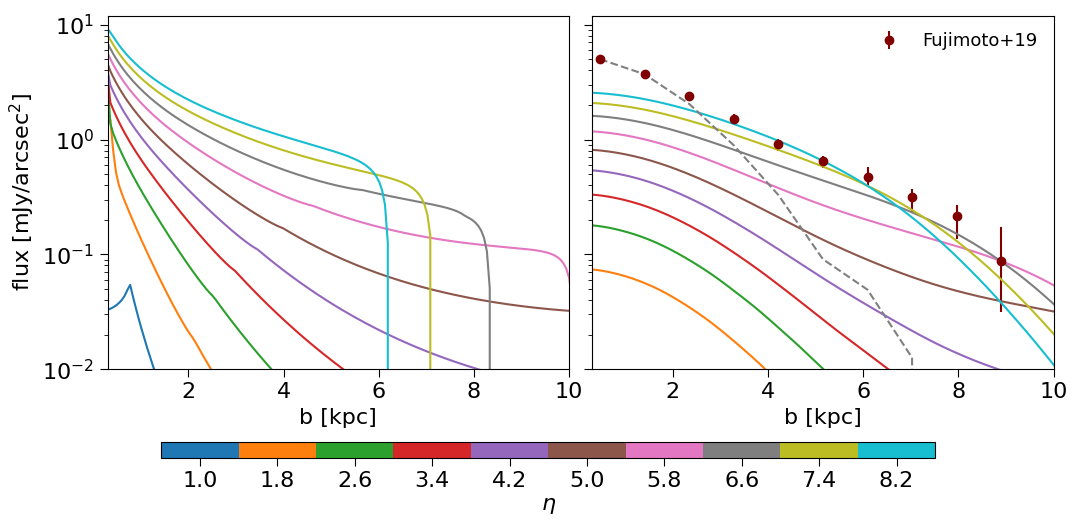
\includegraphics[width=1.0\textwidth]{plots/emission_final.png}
    \caption{\textit{Left}: \CII surface brightness profiles for different values of $\eta$ as a function of the impact parameter $b$. \textit{Right}: comparison of the profiles with data from F19 \citep{Fujimoto19}. The profiles are convolved with the same beam as in the observation (shown with a dashed grey line in the plot).
    \label{fig:global_emission}
    }
\end{figure*}






\begin{comment}


First, however, we briefly explore how these profiles are affected by different choices for our model parameters.


\subsection{Dependence on the halo circular velocity}\label{sec:vc_dependence}

COMMENT ON THE VC DEPENDENCE FURTHER; WHICH PLOTS TO SHOW HERE?


As a final step, we explore the dependence of the results on the dark matter halo circular velocity, $v_c$ (eq. \ref{eq:v_esc}).  We normalize the profiles to the central value of the F19 data to emphasize the differences in the profile shapes.


It is useful to comment on the dependence of \CII emission on $\eta$ and $v_c$. While $\eta$ affects primarily the overall halo brightness by regulating the outflow density, changing $v_c$ is equivalent to modify the strength of the gravitational field. As it is clear from Fig. \ref{fig:vesc_emission}, a deep gravitational potential ($v_c \gtrsim 200\kms$) results in values of $r_{\rm stop}$ which do not match the observed extension of the emitting halo. Weaker potentials ($v_c \simlt 150\kms$) are instead unable to slow down the outflow and therefore maintain a sufficiently high gas density in the outer regions of the halo. In this case, the low density of the gas results in a very faint (undetectable) emission. In addition, the low-density gas is more susceptible to photoionization by the galactic and/or cosmic UV field turning \CIIion into \CIIIion. Such a key role of the gravitational confinement has been noted also in recent hydrodynamical simulations results \citep{li2019supernovae}.


Generally, a tight anti-correlation between $\eta$ and $v_c$ is found, but the likelihood shows a narrow maximum around the values close to the ones identified previously, i.e. $\eta = 3.2 \pm 0.10$ (or $\dot{M}_\mathrm{out}= 128 \,\msun {\rm yr}^{-1}$) and $v_c = 170 \pm 10 \kms$. These results imply that extended halos might be used to set constrains on the mass loading factor and dark matter halo mass of early galaxies.


\begin{figure*}
    \centering
    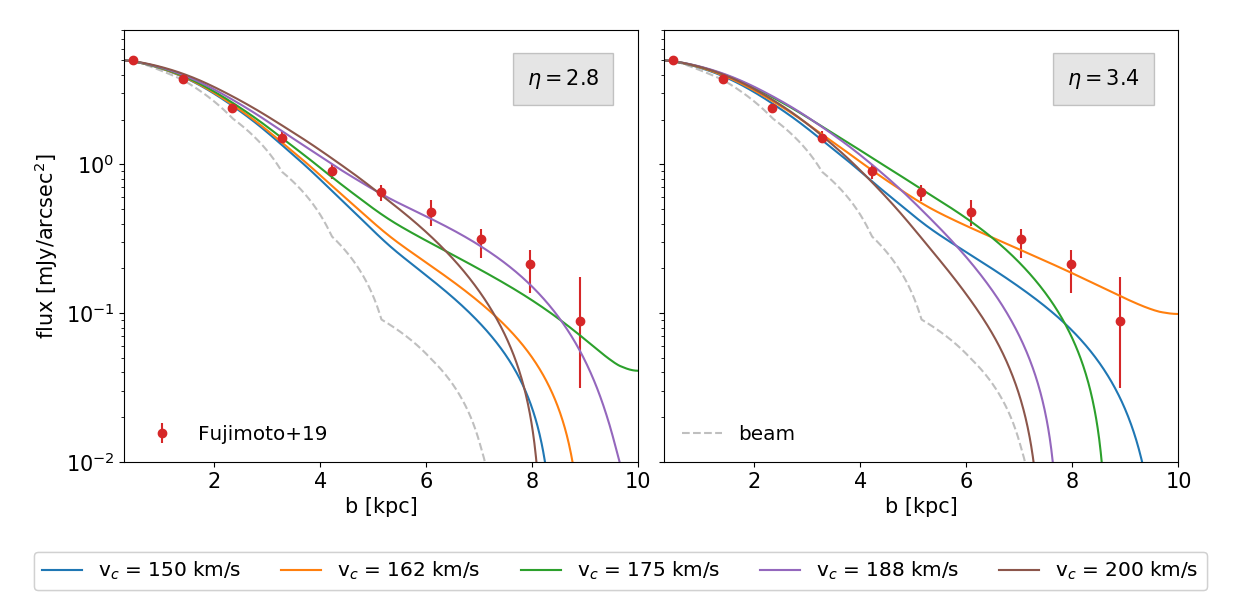
\includegraphics[width=1.025\textwidth,height=8.5cm]{vesc_emission_last.png}
    \caption{Predicted \CII surface brightness profiles (solid lines) as a function of the impact parameter $b$ for different values of the centrifugal velocity $v_\mathrm{c}$, compared with the data from F19 (points). Two values of the mass loading factor are shown: $\eta=2.8$ (left panel), $\eta=3.4$ (right). The profiles are normalised to the central value of the data, and convolved with the same ALMA beam (grey dashed line) used by F19.
    \label{fig:vesc_emission}
    }
\end{figure*}


\subsection{Dependence on metallicity}


 We have run new simulations of our model varying the gas metallicity. In particular, we have taken our best fit parameters ($\eta=3.2$ and $v_c=175$ km/s) and we have changed the metallicity between the two extreme values $Z=0.1, 1$. 
We find that, despite the fact that the cooling function significantly depends on metallicity, the final emission varies roughly linearly with $Z$, and this dependence in the emission is only due to carbon abundance in the gas. 
This is not unexpected, as the emission depends on gas density (and only marginally on gas temperature), on the CII ionization fraction, and on the carbon abundance (eq.s 17-18; NB: due to a typo, eq. 17 was missing an $A_C$ however correctly included in the calculations). Comparing the profiles for Z=0.1 and Z=1, we note that the density behaves similarly, while the temperature profiles are slightly different because of the different cooling functions; in both cases, though, the catastrophic cooling takes place within the first kpc. This means that CII ionization fraction is very similar in the two cases. Therefore, the only residual dependence of the CII emission is on the C abundance. Emission profiles normalized on the metallicity are thus quite similar in the two cases. 
Given this dependence, our best fit model provides a good fit for solar metallicity values. However, a higher mass loading factor and a lower circular velocity might accommodate metallicities as low as $Z=0.1$. Our choice of solar metallicity is motivated by both theoretical (numerical simulations at $z=6$, Pallottini+17,19) and empirical (extrapolation of the mass-metallicity relation for galaxies at $z=6$, Mannucci+12) arguments. 
We have added the corresponding text with this discussion in Sec. 3.2 of the paper. Here, for referee's convenience, we attach three plots: Figure \ref{fig:cooling} shows the cooling functions for the metallicities $Z=1$ and $Z=0.1$, Figure \ref{fig:ionization} shows the carbon ionization fraction in the two cases, and Figure \ref{fig:emission} the emission normalized on the metallicity.




\begin{figure}
	\centering
	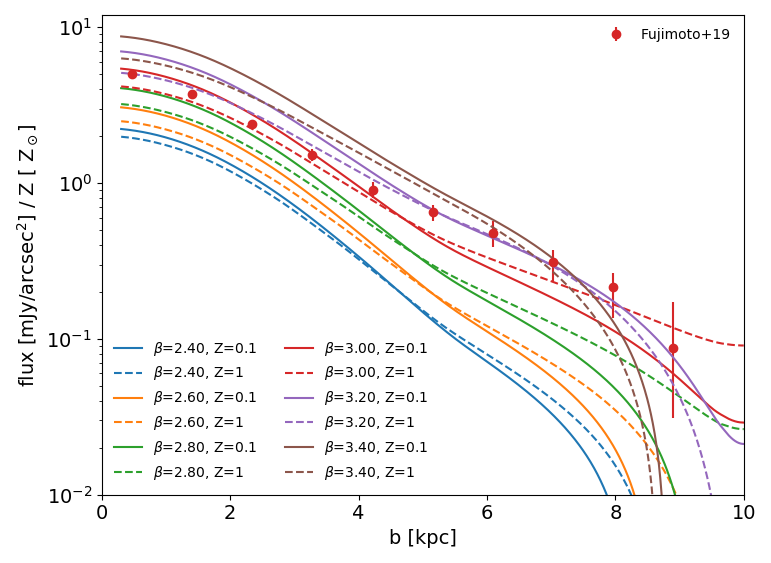
\includegraphics[width=0.8\textwidth]{plots/emission_Zeta_dependence.png}
	\caption{CII emission (as described in the right column of Figure 5 in the paper) for the two values of the metallicites $\mathrm{Z}=0.1$ (lefft) and $\mathrm{Z}=1$ (right). 
	}
	\label{fig:emission}
\end{figure}

\end{comment}





\chapter{Results and comparison with observations} \label{chap:results}
\vspace{20pt}


Having derived the theoretical predictions given by our model, we can take a final step forward by comparing these results with the observational data we presented in chapter \ref{chap:halos}. In particular, we choose to focus on the ALMA ALPINE sample described in section \ref{sec:alpine} (for the original paper, see F20 \citep{Fujimoto:2020qzo}). We select this sample because it is the only study of \CII spatial emission in individual high-z galaxies. \CII emission profiles from individual galaxies are very useful because they allow a comparison between the parameters in our model and the properties of the galaxies considered in the sample. 

The F20 study identifies -- from the original ALPINE sample of 23 galaxies whose \CII emission is located above the $5\sigma$ level -- seven different systems that fall into their "\CII halo" category. By considering this subset of profiles, we run our model with different parameters in order to compare it with the data.
%
Our aim is twofold: on the one hand, we want to use this comparison to determine whether there is good accordance between our theoretical framework and observations. If that were the case, we would have a quantitative argument in favor of the outflows hypothesis as the best candidate to explain the origin of \CII halos.
%
On the other hand, it is interesting to use the data to gauge the values of the parameters in our model. Assuming that outflows are indeed the main source for these high-z halos, in fact, we can draw some interesting conclusions on the physical conditions of high-z galaxies by inferring the best-fit values of the parameters of our model. 

In this chapter, we focus on these different tasks. We start by studying whether our model is able to account for the \CII emission measured by observations (section \ref{sec:single_profiles_comp}). Then, we set up a Markov Chain Monte Carlo (MCMC) simulation in order to infer the posterior probability distribution for the parameters in our model (section \ref{sec:mcmc}). Finally, in section \ref{sec:results}, we discuss our results, also in light of previous theoretical and observational work. 


\section{Comparison with individual profiles} \label{sec:single_profiles_comp}

\subsection{Description of the sample} \label{sec:sample_description}

The sample of "CII Halo" systems identified by F20 consists of seven different galaxies with the following property: considering the emission coming only from a peripheral region (i.e., masking the central galaxy's contribution), the statistical significance of the \CII line must be above the $4\sigma$ level, and, at the same time, (rest-frame) UV and FIR continuum must be below $3\sigma$. To this sample, we add the system DC$494057$, which does not belong to the "\CII Halo" category in F20 as it does not respect the bounds on the FIR/UV continuum luminosities. However, this system has been studied by HC21 \citep{herrera2021kiloparsec} in a follow-up work (sec. \ref{sec:alpine}), showing clear evidence for the presence of a \CII halo and an outflow. 

By combining ALMA observations with ancillary data coming from HST, VLT, and Spitzer, it is possible to measure the different properties of these systems. In particular, the \CII line can give an estimate of the redshift, $z = z_\mathrm{CII}$, and the combined measurements of rest-frame UV and FIR continuum allow a Spectral Energy Distribution (SED) fitting that gives an estimate both of the star formation rate (SFR) and of the stellar mass ($M_\mathrm{star}$). As described in the last chapter, $z$ and $\mathrm{SFR}$ are important parameters in our model. Therefore, these ancillary data can be used to constraint the parameter space we have described in section \ref{sec:outflow_profiles}. 

Another very important quantity that determines the evolution of the wind in our model is the halo virial mass $M_\mathrm{vir}$ (or, equivalently, the global circular velocity $v_c$; see sec. \ref{sec:cooling_gravity}). The halo mass can be linked to the stellar mass via a redshift-dependent function, known as the Stellar Mass-Halo Mass relation (SMHM).
%
As described in section \ref{sec:feedback}, this relation depends on a number of physical processes that are quite difficult to model. However, it is possible to gauge this relation by combining semi-analytical prescriptions for the halos and galaxies growth with observables such as the galaxy luminosity function, the star formation rate history, etc.
%
A great deal of theoretical work has focused on this task, obtaining a satisfactory description of how the SMHM relation evolves with redshift. Here, we use the modeling by \citet{behroozi2013average} to link the stellar mass to the virial mass and to the global circular velocity.

In table \ref{tab:alpine_sample}, we show the properties of the eight systems considered. Overall, these systems are normal, $z \approx 4.5-5.5$, star-forming galaxies, with star formation rates between $10$ and $100\,\msun\,\mathrm{yr}^{-1}$, stellar masses in the range $0.5-1.5 \,\times10^{10}\,\msun$, and, consequently, global circular velocities around $200-250\,\kms$.

\begin{table}
\centering
%
\begin{tabular}{ c c c c c c }
\hline
Name   & $z$    & $\mathrm{SFR}$ [$\msun\,\mathrm{yr}^{-1}$]   & $M_\mathrm{star}$ [$10^{9}\,\msun$]    & $M_{vir}$ [$10^{11}\,\msun$]     & $v_c$ [$\mathrm{km}\,\mathrm{s}^{-1}$] \\ 
\hline
\hline
DC$396844$    &    $4.54$    &    $55^{+40}_{-25}$    &   $7.3^{+2.6}_{-2.6}$   &   $4.1^{+2.8}_{-1.8}$    &   $206^{+90}_{-66}$ \\
DC$494057$   & $5.54$   &    $42^{+35}_{-15}$    &   $14.2^{+4.9}_{-4.2}$   &   $6.7^{+5.2}_{-3.5}$    &   $263^{+133}_{-97}$\\
DC$630594$    &    $4.44$    &    $31^{+24}_{-15}$    &   $5.9^{+2.3}_{-1.7}$   &   $3.6^{+2.6}_{-1.5}$    &   $196^{+85}_{-59}$ \\
DC$683613$    &    $5.54$    &    $58^{+44}_{-26}$    &   $14.7^{+5.7}_{-4.4}$   &   $7.0^{+5.9}_{-3.7}$    &   $267^{+145}_{-102}$ \\
DC$880016$    &    $4.54$    &    $32^{+25}_{-15}$    &   $5.6^{+2.3}_{-1.6}$  &   $3.5^{+2.6}_{-1.4}$    &   $196^{+85}_{-58}$ \\
DC$881725$    &    $4.58$    &    $88^{+61}_{-43}$    &   $9.1^{+4.0}_{-2.1}$   &   $4.8^{+3.5}_{-2.1}$    &   $217^{+98}_{-68}$  \\
VC$5100537582$    &    $4.55$    &   $15^{+14}_{-6}$    &   $5.7^{+2.0}_{-1.6}$  &   $ 3.6^{+2.5}_{-1.5}$    &   $197^{+83}_{-58}$ \\
VC$5110377875$    &    $4.55$    &    $99^{+79}_{-41}$    &   $14.7^{+4.7}_{-5.6}$   &   $7.0^{+5.1}_{-3.9}$    &   $246^{+125}_{-97}$ \\
 \hline
\end{tabular}
%
\caption{Properties of the "CII Halo" sample taken from the F20 study \citep{Fujimoto:2020qzo}. From left to right: name of the ALPINE source ("DC" stands for "DEIMOS COSMOS", while "VC" stands for "VUDS COSMOS"), redshift ($z$), Star Formation Rate ($\mathrm{SFR}$), stellar mass ($M_\mathrm{star}$), halo mass ($M_{vir}$), and global circular velocity ($v_c$). Uncertainties on the redshift measurements are very small and not shown here. 
\label{tab:alpine_sample}
}
\end{table}

\subsection{$\chi^2$ test} \label{sec:chi2}

\begin{figure*}[t]
    \centering
    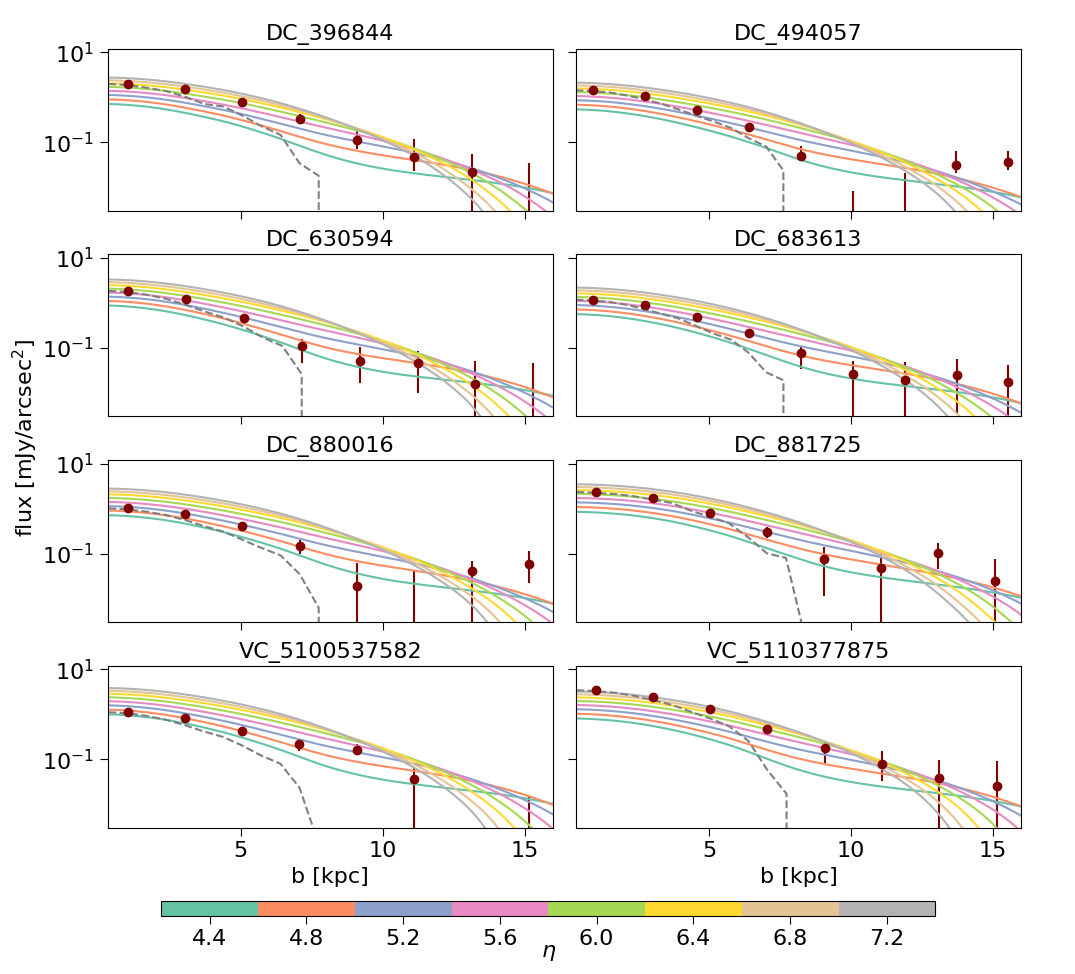
\includegraphics[width=1.0\textwidth]{plots/single_profile_emission.png}
    \caption{Comparison of the \CII profiles obtained by using the model presented in chapter $\ref{chap:model}$ (colored lines) with data from the F20 "\CII Halo" sample (red dots). All parameters are fixed according to observations (table \ref{tab:alpine_sample}), except for the mass loading factor $\eta$ which is varied in the plots. The profiles are convolved with the same beams as in the observations (shown with dashed grey lines in the plots).
    \label{fig:single_profiles}
    }
\end{figure*}


\begin{table}
\centering
%
\begin{tabular}{ c c c }
\hline
Name      & $\chi^2_\mathrm{min}(d|\eta)$  & $\eta_\mathrm{min}$  \\ 
\hline
\hline
DC$396844$      &    $12.6$  &    $5.5$ \\
DC$494057$      &    $8.6$  &    $8.4$ \\
DC$630594$      &    $20.9$ &    $6.4$  \\
DC$683613$      &    $3.6$ &    $5.3$   \\
DC$880016$     &    $10.0$  &    $5.9$  \\
DC$881725$    &    $17.5$  &    $4.0$    \\
VC$5100537582$   &   $16.9$   &    $8.2$   \\
VC$5110377875$    &    $45.6$  &    $4.3$   \\
 \hline
\end{tabular}
\caption{Results for the $\chi^2$ test for the F20 \citep{Fujimoto:2020qzo} (sub-)sample here considered. ALPINE source names are listed in the first column (see also table \ref{tab:alpine_sample}); the second column refers to the minimum value of $\chi^2(d|\eta)$ with respect to the mass loading factor, whose minimizing value $\eta_\mathrm{min}$ is shown in the third column. Details of the model-data comparison can be found in the text and in figure \ref{fig:single_profiles}. 
\label{tab:alpine_chi2}
}
\end{table}

For each system, we can take as fiducial value the one obtained by table \ref{tab:alpine_sample}. As a result, if we also assume (as argued in section \ref{sec:outflow_profiles}) $Z= 1\,Z_\odot$ and $\fesc=0$, the only residual parameter in our model is the mass loading factor $\eta$. For this reason, as a first investigation, we study how the model compares with the data for different values of the $\eta$ parameter. Figure \ref{fig:single_profiles} shows how our model compares with the F20 sample: observational data are plotted, together with the emission profiles resulting from our outflow model, for different values of $\eta$. These profiles are created by using the observational estimates for redshift, SFR, circular velocity, and FWHM of the \CII line, and they are also convolved with the same beam as observations. 

Almost all the plots in figure \ref{fig:single_profiles} indicate a good level of accordance between the data and our model. To base our comparison on quantitative arguments, we introduce a $\chi^2$ statistics as a measure of the "\textit{goodness of fit}" for our theoretical model. The $\chi^2$ for a set of $n$ data $d=\{y_i(x_i)\pm\sigma_i\}_{i=1}^n$ and a model $m$ (depending on a parameter $\eta$), is defined as:
\begin{align}
    \chi^2(d | \eta ) = \sum_{i=1}^n \frac{(y_i - m(x_i;\eta))^2}{\sigma_i^2}
\end{align}
If we assume that: (a) different measurements are independent; (b) the errors $\sigma_i$ have Gaussian distributions; and (c) the errors on the quantities $x_i$ are negligible; then, we expect the random variable $\chi^2(d | \theta )$ to be distributed just as a $\chi^2$ with $n-1$ degrees of freedom (i.e., as a squared sum of $n-1$ normal Gaussian variables). A $\chi^2$ with $n-1$ degrees of freedom has an expectation value $E(\chi^2) = n-1$, and a variance $\sigma^2({\chi^2})=2(n-1)$.

For the F20 sample, the hypotheses on which the $\chi^2$ test is founded are valid. Therefore, running the test on the sample, we should recover in principle extractions from a $\chi^2$ distribution with a number of data per set of $n=9$. However, we caution the reader that this discussion has some limitations. In fact, we do not expect the results of a $\chi^2$ test to be fully accurate in the case here considered, for a variety of reasons. Most importantly, our model has several limitations: many assumptions we have made (e.g., spherical symmetry, time stationarity, very crude treatment of the central galaxy) are expected to cause important variations on the data profiles and/or fluctuations. %Therefore, we need to be aware of the limitations of our model when interpreting how it compares with data.

For instance, the fact that the central emission is not well modeled in our framework has important consequences in the computation of the $\chi^2$, as the errors of the central data points are the smallest ones (because of their higher S/N). Thus, even profiles that, overall, are in good agreement with the data can have a relatively high $\chi^2$. Further discussion on limitations and possible improvements is left for the final chapter (chap. \ref{chap:conclusion}). Nonetheless, the values of the $\chi^2$ can be considered as a first, approximated way to determine whether there are values of $\eta$ for which the accordance of the model with the F20 profiles reach a satisfactory level. With this respect, we display in table \ref{tab:alpine_chi2} the minimum value of $\chi^2(d|\eta)$ for each of the F20 profiles considered, and the corresponding value of the $\eta$ parameter which corresponds to  $\chi^2_\mathrm{min}(d|\eta)$.

For most of the systems, good accordance is found between the model and the data profile for values of $\eta$ ranging from $\eta\approx 4$ o $\eta \approx 8$.
%
The only notable exception is VC$5110377875$: in this case, the flux in the central region is particularly intense, and the only values of $\eta$ that are compatible with similar values of the emission in the central regions are $\eta \approx 7-8$; these same values, however, are not compatible with the extension of the halo in the external regions of the CGM, as they are slowed down by gravity and their emission drops at distances that are too small compared with the data. In the same way, lower values of $\eta$ are too faint for the central emission but are faithfully representing the outer regions of the halo. With this respect, we note that a missing contribution from the central ISM (discussed at the end of section \ref{sec:CII_emission}) could alleviate the conflict between model and data. 

\subsection{$\mathrm{SFR}$ and $v_c$ dependences}

\begin{figure*}
    \centering
    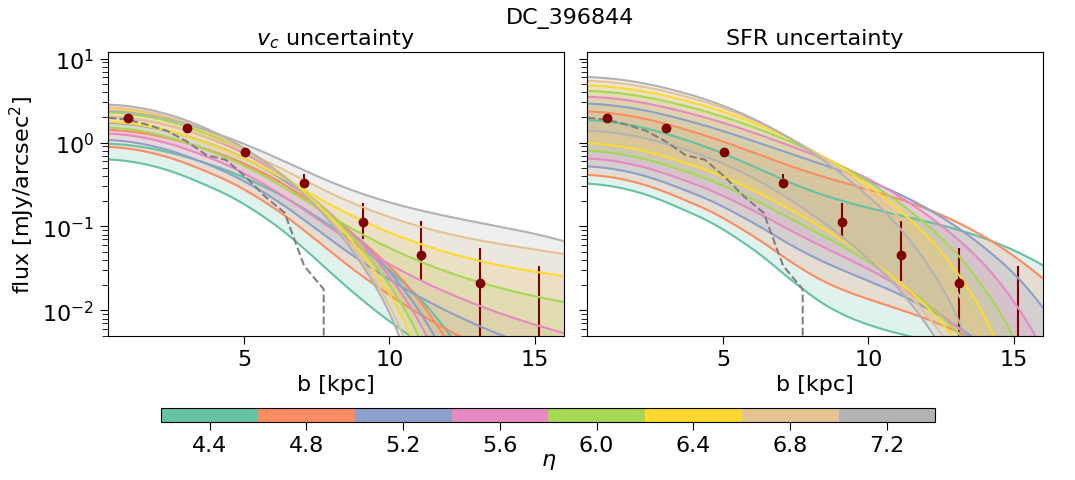
\includegraphics[width=1.0\textwidth]{plots/vc_sfr_emission.png}
    \caption{Same comparison between theoretical profiles and observational data, as in figure \ref{fig:single_profiles}. The DC$396844$ system is considered for illustrative purposes. \textit{Left}: the lower and higher limits for the global circular velocity $v_c$ -- as inferred from observations -- are considered. All the other parameters are fixed to their observational best estimate (table \ref{tab:alpine_sample}), while the mass loading factor $\eta$ is varied in the plot. For every value of $\eta$, the profiles corresponding to $v_{c,\mathrm{min}}$ and $v_{c,\mathrm{max}}$ are plotted, and the region between them is shaded accordingly. \textit{Right}: same as the left panel, but the star formation rate is considered. Profiles are created by setting the SFR equals to $\mathrm{SFR}_\mathrm{max}$ and $\mathrm{SFR}_\mathrm{min}$, as inferred by observations (table \ref{tab:alpine_sample}). 
    \label{fig:sfr_vc_unc}
    }
\end{figure*}

The $\chi^2$ analysis has shown that a good fraction of the systems considered is well-fitted by our single-parameter models. We could go further in our analysis by studying, e.g., the error associated with the best-fit values of $\eta$. However, we choose to follow another approach, as we realize that a single-parameter model has some intrinsic limitations that can bias our final results.
%
The reason for that can be appreciated by looking at table \ref{tab:alpine_sample} (see also figure \ref{fig:alpine_trends}): the relative errors on the values of the circular velocity and the star formation rate, as derived from observations, are as high as $50 \%$ both for $v_c$ and SFR -- redshift measurements, instead, are very precise.
%
Such uncertainties can have significant implications for our choice of parameters. We can appreciate this by studying the dependence of the final emission profiles on $v_c$ and on $\mathrm{SFR}$. 

Changing the value of $v_c$ is equivalent to modifying the gravitational pull acting on the outflowing gas. This alters the evolution of the wind quite considerably: increasing $v_c$, the gas velocity $v$ decreases (in particular in the outer regions), and, consequently, its density $n$ tends to increase. Ultimately, these changes result in a smaller stalling radius $r_\mathrm{stop}$, and hence in a different extension of the gaseous halo formed by the wind.
%
The effects of these changes on the final, convolved, \CII emission profiles are quite difficult to quantify, as opposite trends are at play: higher densities imply a higher \CII emission, but at the same time, smaller stalling radii results in an emission that drops earlier and thus it is not as strong in the outer regions of the CGM.

In order to see whether these expected trends have a measurable impact on our final results, we study how $v_c$ affects the final \CII emission profiles in figure \ref{fig:sfr_vc_unc} (left panel). In particular, we consider the same \CII emission profiles that we have shown in figure \ref{fig:single_profiles}, i.e., focusing on the system DC$396844$.
%
In this case, however, we consider different values for the circular velocity $v_c$: we plot the lower and the upper fiducial bounds that can be inferred from observations (table \ref{tab:alpine_sample}). We highlight the differences between these two choices by filling in the region between the two profiles. As in figure \ref{fig:single_profiles}, we repeat this procedure for different choices of the mass loading factor $\eta$, color-coding the results accordingly. The resulting plot implies that, indeed, our model is quite sensitive to the value of the global circular velocity selected, and observations alone cannot provide us with the best choice for $v_c$ because of the relatively large uncertainties of the measurements. 

These conclusions are even more dramatic if we consider the dependence of the \CII profiles on the star formation rate. For $\fesc = 0$, the set of equations governing the wind evolution (eqs.\ref{eq:cooling_model_equations}) does not depend on the SFR. Even so, the SFR affects the outflow profiles because it determines the boundary conditions for the wind (eqs. \ref{eq:boundary}).
%
In particular, it holds: $n(R) \propto \mathrm{SFR}\,\eta^{3/2}$. As the density is the most important quantity determining the final \CII emission, changing the SFR is expected to have similar effects as changing the mass loading factor $\eta$. The right panel of figure \ref{fig:sfr_vc_unc} validates these expectations: as done for $v_c$, we plot the \CII emission profiles for the system DC$396844$ setting $\mathrm{SFR}_\mathrm{min}$ and $\mathrm{SFR}_\mathrm{max}$ as inferred by observations (table \ref{tab:alpine_sample}). Given the large relative uncertainties on SFR measurements, the data fall mostly inside the shaded regions for all the $\eta$ values considered. 

The analysis here presented suggests that it is necessary to expand the parameter space considered in the comparison with data, in particular including the star formation rate and the global circular velocity as parameters; this is the goal of the next section, where we still use observations to guide our exploration of the parameter space, but we do not restrict ourselves to fixed values of $\mathrm{SFR}$ and $v_c$.

\section{MCMC analysis} \label{sec:mcmc}

\begin{figure*}
    \centering
    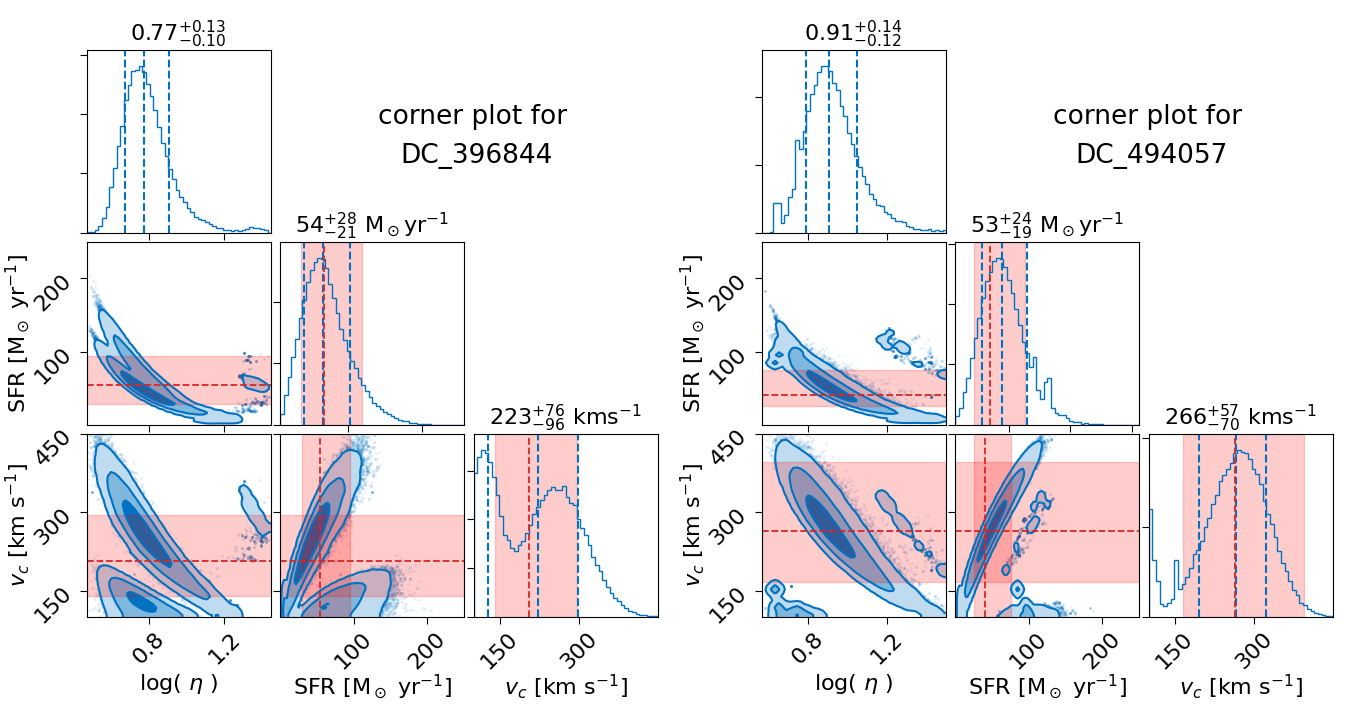
\includegraphics[width=1.0\textwidth]{plots/corner_final_1.png}
    \caption{Corner plots (i.e., 1-d and 2-d marginalizations) of the 3-d posterior distribution $P(\Theta|d,m)$, with $\Theta = \{\log\eta, \mathrm{SFR}, v_c\}$. The posterior distribution was sampled using an MCMC algorithm, set up with the Python package \code{emcee} (details in the text). Two out of the eight F20 "\CII Halo" systems are shown here (the other ones are shown in figure \ref{fig:corner_2}). The values of the parameters $\mathrm{SFR}$ and $v_c$, as inferred from observations (table \ref{tab:alpine_sample}), are shown with red dashed lines, together with their uncertainties (red shaded regions). The blue dashed vertical lines represent the median and $1\sigma$ errors on the parameters: these same quantities are also shown at the top of each 1-d histogram. 
    \label{fig:corner_1}
    }
\end{figure*}

From the discussion in the last section, it follows that the parameter space needs to be extended by including $\mathrm{SFR}$ and $v_c$. In principle, we could minimize the new, multi-dimensional $\chi^2$ distribution $\chi^2(d|\eta, \mathrm{SFR}, v_c)$ to find the best-fitting parameters, just as we did in section \ref{sec:single_profiles_comp}.
%
However, it is convenient at this point to introduce a more general framework for two main reasons: (a) we still want to exploit in our analysis the values of the star formation rates and of the global circular velocity inferred from observations; (b) we want to associate an uncertainty to the best-fitting values of the parameters.

\subsection{The Bayesian framework} \label{sec:bayes}

The setting of the Bayesian framework is the same we have already considered in section \ref{sec:single_profiles_comp}: a theoretical model $m(\Theta)$ (depending on a set of parameters $\Theta$) is to be compared with some data $d=\{y_i(x_i)\pm \sigma_i\}$.
%
In the Bayesian approach, however, the question one seeks to answer is different: which is the probability distribution associated with the set of parameters $\Theta$ that can be inferred from the comparison with data?
%
Bayes theorem allows to write this distribution (known as "posterior"), $P(\Theta|d,m)$, in terms of two other quantities: a "prior" distribution $\pi(\Theta|m)$, expressing the a-priori (i.e., not coming from the data) information on the parameters, and a "likelihood" $\mathcal{L}(d|\Theta,m)$, describing the probability of obtaining the set of data $d$ assuming a fixed set of parameters $\Theta$. The Bayes theorem reads:
\begin{equation}
    P(\Theta\,|d,m) = \frac{\pi(\Theta|m)\,\mathcal{L}(d\,|\Theta, m)}{\mathcal{Z}(d|m)},
\end{equation}
where $\mathcal{Z}(d|m)= \int \d \Theta\,\pi(\Theta)\,\mathcal{L}(d\,|\Theta, m) $ (dubbed as "evidence") can be considered a normalization constant.

Under the same hypotheses as section \ref{sec:chi2} (i.e., independence between different measurements, Gaussianity of statistical errors), it can be proven \citep[e.g.,][]{jaynes_2003} that the likelihood is a function of $\chi^2$:
\begin{equation}
    \mathcal{L}(d\,|\Theta, m) = e^{-\chi^2(d|\Theta)} = \exp\left(-\sum_{i=1}^n \frac{(y_i - m(x_i;\eta))^2}{\sigma_i^2}\right)
\end{equation}
Therefore, maximizing the likelihood is the same as minimizing the $\chi^2$: in this sense, the Bayesian approach and the $\chi^2$ formalism are equivalent. An important difference, however, is played by the prior term $\pi(\Theta|m)$. In fact, this quantity can alter the final shape of the posterior distribution in a way that the $\chi^2$ approach is not able to capture. 

In this analysis, we have chosen to focus on three parameters: the mass loading factor $\eta$, the star formation rate (SFR), and the global circular velocity $v_c$. Therefore, we need to specify the priors for these quantities.
%
The a-priori knowledge we have on these parameters varies. The mass loading factor is largely unconstrained both theoretically and observationally: even its order of magnitude is quite unclear, ranging from $\eta \lesssim 0.1$ to $\eta \gtrsim 10$ \citep[e.g.,][]{muratov2015}. For this reason, the most suitable prior for $\eta$ is a logarithmic prior (i.e., a uniform prior for $\log \eta$). Therefore, from now on we work with the parameter $\log \eta$, assigning to it a uniform prior in the range $-1 < \log\eta < 1.5$. On the other hand, both $\mathrm{SFR}$ and $v_c$ are constrained by our general knowledge of high-z galaxies; moreover, the ancillary data in table \ref{tab:alpine_sample} give even more accurate estimates for their values. For this reason, we choose to set Gaussian priors for these two quantities, centered in their fiducial values inferred from observations, and with a standard deviation equal to half of the total (upper+lower) error of these measured values.

Overall, the prior distribution we consider is null outside the region $-1 < \log\eta < 1.5$, while inside this region it equals to ($\Delta(\log\eta) = 2.5$):
\begin{equation}
    \pi(\Theta|m) =  \frac{1}{\Delta(\log\eta)}\frac{1}{2\pi\sigma_{\mathrm{SFR},i}\sigma_{v_c,i}}\exp\left(-\frac{\left(\mathrm{SFR}-\mathrm{SFR}_i\right)^2}{2\sigma_{\mathrm{SFR},i}^2}-\frac{\left(v_c-v_{c,i}\right)^2}{2\sigma_{v_c,i}^2}\right),
\end{equation}
where $\mathrm{SFR}_i \pm \sigma_{\mathrm{SFR},i}$ and $v_{c,i} \pm \sigma_{v_c,i}$ refers to the values displayed in table \ref{tab:alpine_sample}.

\subsection{Setting up MCMC runs}

\begin{figure*}[t]
    \centering
    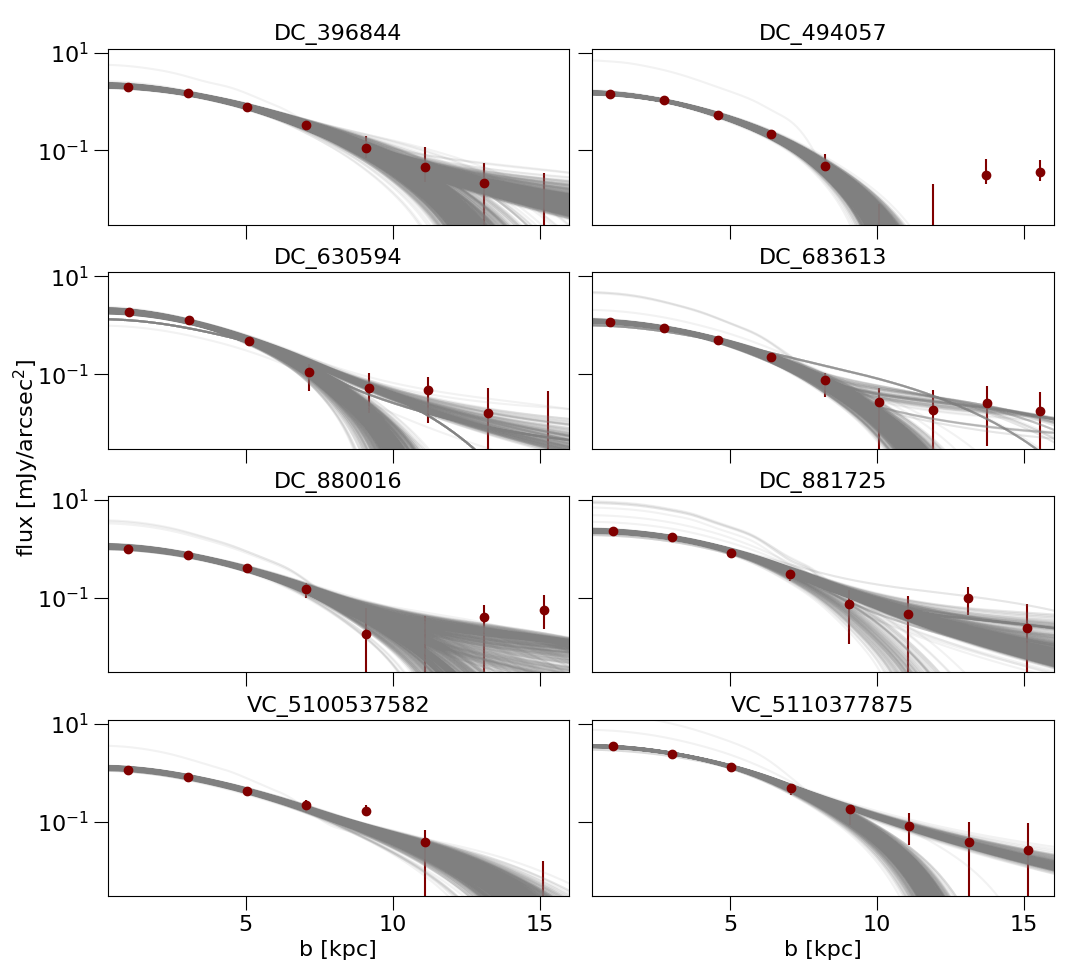
\includegraphics[width=1.0\textwidth]{plots/mcmc_emission.png}
    \caption{Comparison of the \CII profiles obtained by using the model presented in chapter $\ref{chap:model}$ (light gray lines) with data from the F20 "\CII Halo" sample (red dots). The profiles are created by choosing $10^3$ different values of the parameters, extracting them randomly from the MCMC chains ($\{\Theta_i\}_{i=1}^N$) obtained in section \ref{sec:mcmc}. The profiles are convolved with the same beams as in the observations (shown in figure \ref{fig:single_profiles}).
    \label{fig:mcmc_emission}
    }
\end{figure*}

Once the priors are set, the posterior distribution is well-defined, and it can be computed at any point of the parameter space. The most naive approach that can be followed to describe the global behavior of the posterior is to build a grid in the parameter space and to compute the posterior for every point in the grid. However, this approach gets more and more problematic as the dimensions of the parameter space increase. Already in 3-D, techniques based on stochastic samplers become competitive. The idea behind this alternative approach is to generate a list of $N$ posterior samples $\{\Theta_i\}_{i=1}^N$ drawn from the parameter space, such that the number of samples on the region $\Theta + \Delta \Theta$ ($\Delta \Theta \ll \Theta$) is proportional to $P(\Theta|d,m)$. 

The most popular class of samplers is represented by the Markov Chain Monte Carlo (MCMC) algorithms \citep{metropolis, hastings}. In MCMC methods, a set of $m$ particles (dubbed as "walkers") move randomly in the parameter space. At each step, the probability for a particle to move to any given point is determined by a Markov chain, that is created following several possible prescriptions; these prescriptions aim to generate new samples according to the posterior distribution.
%
By recording the positions of the walkers at each iteration, "chains" of elements $\{\Theta_i\}_{i=1}^N$ are created. These chains can be thought of as draws from the posterior probability distribution; therefore, a simple histogram of the elements in the chains reveals the shape of the posterior. Of course, the first elements of every chain need to be discarded because they depend on the chain's initial conditions (this is the so-called "burn-in" phase). Additionally, there are inevitable correlations between the position of a walker at a given step in the chain and its positions at the following/preceding steps. These correlations can be averaged to give the "autocorrelation time" $\tau$. It is important to check that this autocorrelation time does not exceed a small fraction of the full length of the chain; if it does, its effects need to be accounted for, as the width of the distribution gets underestimated because of correlations.

%It is also beneficial to run many different walkers starting from different regions of the parameter space, as a single walker can fail to find multiple modes of a posterior distribution if there are regions of low posterior probability between the modes. 

Here, we do not describe the details of different algorithmic prescriptions, nor do we analyze the many other subtleties that must be considered when dealing with MCMC samplers \citep[for a review on this, see e.g.,][]{sharma2017markov}. Instead, we limit ourselves to describe the general setup that we choose for our analysis: we use the well-known code \code{emcee} \citep{foreman2013emcee} to run an MCMC using the affine-invariant ensemble prescription to generate new samples \citep{goodman_prescription}. For each system considered (table \ref{tab:alpine_sample}), we run the MCMC algorithm by placing $m=96$ walkers distributed randomly in the parameter space and evolving them for $N=10^5$ steps. We discard the first $10^3$ elements to account for the burn-in phase, and we thin the chain considering only one element every $\tau$ steps in order to account for autocorrelations. The results of these runs are described in the next section.

\section{Discussion} \label{sec:results}

\begin{figure*}
    \centering
    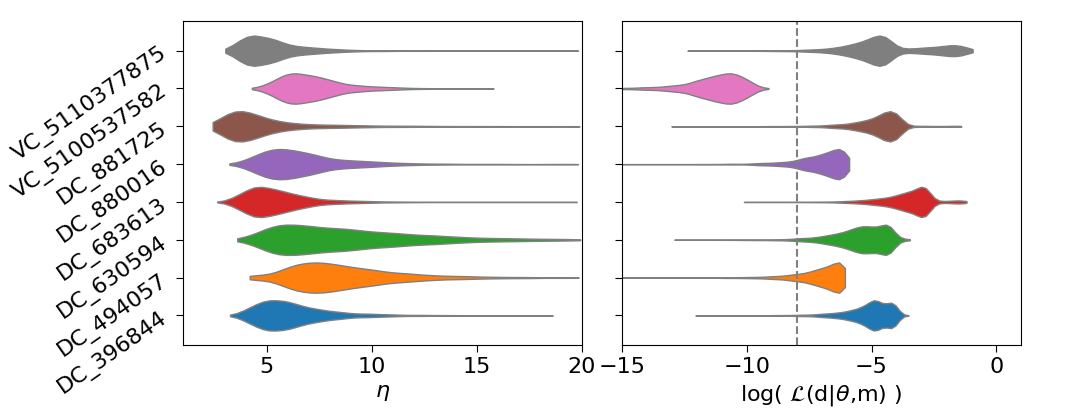
\includegraphics[width=1.0\textwidth]{plots/violin_new.png}
    \caption{\textit{Left}: violin plot representing the 1-d marginalized posterior distributions for the parameter $\eta$. Posteriors are obtained from the MCMC runs described in section \ref{sec:mcmc} \textit{Right}: violin plot representing the probability distribution associated with the natural logarithm of the likelihood term, $\log( \mathcal{L}(d|\Theta,m))$; in our setup, this term equals to $-\chi^2(d|\Theta)$. The gray dashed line shows the expectation value of $-\chi^2$ (see section \ref{sec:chi2} for more details).
    \label{fig:violin}
    }
\end{figure*}



Figure \ref{fig:corner_1} and figure \ref{fig:corner_2} show the "corner plots" for the MCMC runs described in the last section. Every set of plots refers to one of the systems of the "\CII Halo" F20 sample. Corner plots show the various combinations of 1-d and 2-d distributions of the chains $\{\Theta_i\}_{i=1}^N$ obtained from the different runs; mathematically, they represent the 1(2)-d posterior distributions obtained by marginalizing over all the parameters except for one (two) at a time.
%
Therefore, the 1-d histograms are the probability distributions for the single parameters: $\log\eta$, $\mathrm{SFR}$, and $v_c$. From these distributions, the median values and the $1\sigma$ errors (i.e., the $16^\mathrm{th}$ and $84^\mathrm{th}$ percentiles) can be obtained: these are the best estimates for the parameters that we can achieve with our data-model comparison -- they are shown at the top of every 1-d histogram in the figures.

Red shaded regions in figs. \ref{fig:corner_1}, \ref{fig:corner_2} highlight the observational bounds for $\mathrm{SFR}$ and $v_c$. All corner plots show distributions for these two parameters that are perfectly compatible with these bounds. This does not come as a surprise, since our choice for the priors biases the distributions towards the interval gauged by observations. It is interesting to note, however, that there is evidence for a bimodal shape of the posterior distribution, especially for the 1-d posterior on the $v_c$ parameter.
%
The origin of this bimodality can be investigated by looking at figure \ref{fig:mcmc_emission}: in these plots, we generate emission profiles by considering sets of values for the parameters extracted randomly from the MCMC chains. We note that two behaviors are possible: low-$v_c$ profiles form halos that are even more extended than the observational data, while higher $v_c$ values result in an emission that is less extended and barely compatible with the observed one. From the data available, there is no specific preference for any of the behaviors.

The distributions for the $\log \eta$ parameter, instead, are much more interesting, as they are not constrained by our priors choice. We show these distributions for different systems (using the parameter $\eta$ instead of $\log\eta$) in the form of a violin plot in figure \ref{fig:violin}. We obtain median values of $\eta$ in the range $\eta \approx 4-7$. These values are compatible with the ones obtained by using the $\chi^2$ test in section \ref{sec:chi2}. This implies that our Bayesian analysis supports the results we have already obtained with a simple best-fitting approach. The substantial difference lies in the fact that now we are able to assign uncertainties to the inferred values of $\eta$: we find $1\sigma$ errors of the order of $1-3$. 

Another important quantity to look at -- that cannot be easily inferred from the corner plots -- is the value of the likelihood $\mathcal{L}(d|\Theta,m)$. This quantity is relevant since it is a way to measure the "goodness of fit", i.e., the accordance between our model and the observational data. In the right panel of figure \ref{fig:violin}, we plot the probability distributions of $\log(\mathcal{L}(d|\Theta,m))$ (again using a violin plot). As pointed out in section \ref{sec:bayes}, under the hypotheses here considered, the logarithm of the likelihood is simply the inverse of the $\chi^2$. Therefore, the minimum value for $|\log(\mathcal{L}(d|\Theta,m))|$ is the result we would obtain with a $\chi^2$ test. From figure \ref{fig:violin}, we see these values are small for most of the systems, even smaller than the expected value of $\chi^2=n-1=8$ (however, see discussion in sec. \ref{sec:chi2} on the limits of the $\chi^2$ test in this context). Such small values mean that our models are good fits for the data. This can be inferred also by looking at figure \ref{fig:mcmc_emission}: most of the profiles are in very good agreement with the observational data, particularly in the internal regions, where data points have smaller relative errors. These results imply that the Bayesian approach improves our quantitative analysis substantially and that the conclusions we can draw from this model-data comparison are founded on solid grounds.

Finally, in figure \ref{fig:eta_sfr_vc}, we plot the values of $\eta$ inferred by our analysis against the observed values of the stellar mass $M_\mathrm{star}$ (left panel) and of the star formation rate (SFR) (right panel). In both these plots, we fit lines in bilogarithmic scale in order to search for power-law dependences of the form $y=a\,x^b$. 

We exclude from the fit the system DC$494057$ -- that does not belong to the "\CII Halo" class in F20 \citep{Fujimoto:2020qzo} -- because it is a clear outlier in the plots.
%
The reason for this could be the (highly) non-monotonic profile of the DC$494057$ data points: also looking at figure \ref{fig:single_profiles}, we note how our model struggles to capture the complex behavior of the external points. 

We find that both $\eta-M_\mathrm{star}$ and $\eta-\mathrm{SFR}$ are inversely correlated, with the following best-fit parameters ($\log \eta = a_\mathrm{mstar} + b_\mathrm{mstar} \log( M_\mathrm{star}/10^{10}\msun) =  a_\mathrm{SFR} + b_\mathrm{SFR} \log( \mathrm{SFR} /\msun\,\mathrm{yr}^{-1})$):
\begin{align}
    a_\mathrm{mstar} &= 5.1\pm0.4 & b_\mathrm{mstar} &= -0.38\pm0.17      \\
    a_\mathrm{SFR} &= 10.0\pm2.1 & b_\mathrm{SFR} &= -0.13\pm0.07
\end{align}
Therefore, our model suggests that mass loading factors for high-z, normal star-forming galaxies lie in the range $\eta\approx3-10$ (accounting for the statistical uncertainties), with higher values for low-mass and low-SFR systems.

\subsection{Comparison with previous works} 


It is interesting to quantitatively compare our conclusions with other previous works on galactic outflows. Despite the fact that mass loading factors cannot be constrained with high accuracy from observations (chapter \ref{chap:outflows}), there exist some estimates for $\eta$ both locally and at high-redshift that can help us to put our results in the right context.

A seminal work by \citet{Heckman15} uses UV absorption lines to study the properties of SF-driven outflows in local starburst galaxies; the authors of the study find that the mass loading factor correlates weakly and inversely both with $\mathrm{SFR}$ and $v_c$ (or, equivalently, $M_\mathrm{star}$). They identify values for $\eta$ ranging from $1 \lesssim \eta \lesssim 4$: this range of values is lower than the one we find in our study, even though there is a partial overlap. This tension may be due to the fact that hidden (faint) AGN activity may contribute to power outflows in the ALPINE galaxies. This hypothesis is appealing because AGN-driven outflows, being more powerful and disruptive, are characterized by higher values of the mass loading factors \citep[see e.g.,][]{Fiore_2017,fluetsch2019cold}. 

However, we also note that a number of other studies find values for $\eta$ that are significantly higher, and thus compatible with our conclusions. For instance, using H$\alpha$ emission lines originating in the CGM of local galaxies, \citet{zhang2021empirical} measure the mass loading factor for different ranges of halo masses. In the range we are interested in, their result is $2 \lesssim \eta \lesssim 7$, which is in very good agreement with the values we have found.

At high redshifts, the analysis of the broad-wing feature identified by G20 \citep{ginolfi:2019} in the ALPINE star-forming sample (section \ref{sec:alpine}) gives an estimate for $\eta\approx 0.5-2$. However, the HC21 work \citep{herrera2021kiloparsec} (section \ref{sec:alpine}), studying the DC$494057$ system, find similar values for the total mass loading factor only on a global level. In fact, they are also able to resolve the regions where the outflow originates and to compute local values of $\eta$; they find $\eta = 3-6$, which is compatible with our results. This also suggests that measurements of the mass loading factors could be underestimated because of the locality of outflow launching sites. 

\begin{figure*}
    \centering
    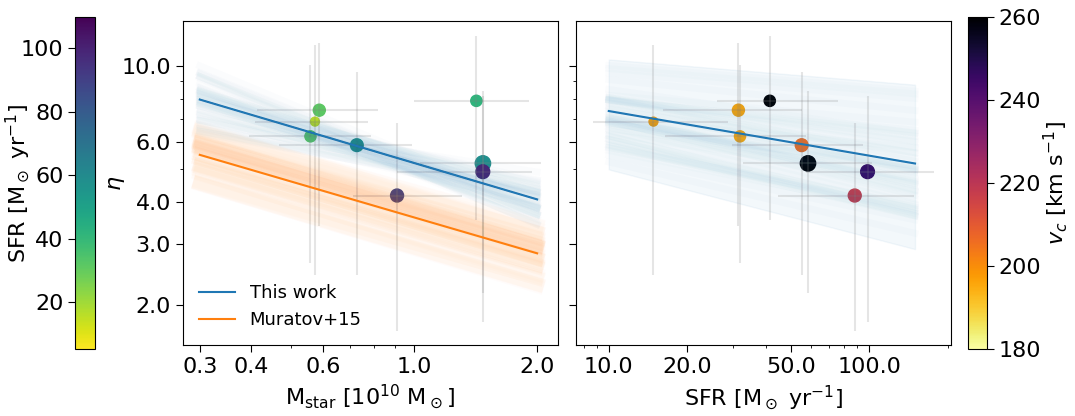
\includegraphics[width=1.0\textwidth]{plots/final_comparison_new.png}
    \caption{\textit{Left}: dependence of the mass loading factor $\eta$ on the stellar mass $M_\mathrm{star}$. The values of $\eta$ plotted are the medians and the $1\sigma$ errors of the 1-d probability distributions obtained from the MCMC analysis (figure \ref{fig:violin}). Stellar masses are inferred from observational data (table \ref{tab:alpine_sample} or figure \ref{fig:alpine_trends}). We fit a power law (i.e., a line in logarithmic scale) in blue to highlight the global trend revealed by our comparison, and we also show previous results from \citet{muratov2015} for reference. Data points are color-coded according to their SFR, as inferred from observations. The size of every point is proportional to its likelihood $\mathcal{L}(d|\Theta,m)$ (figure \ref{fig:violin}). \textit{Right}: dependence of the mass loading factor $\eta$ on the star formation rate (SFR). The same considerations as for the left panel apply. The color of the data points expresses their global circular velocity $v_c$, which is a function of the stellar mass via the SMHM relation (see section \ref{sec:sample_description} for more details). 
    \label{fig:eta_sfr_vc}
    }
\end{figure*}


Simulations have the capabilities to measure mass loading factors much more directly, as well as to study their evolution with redshift and their dependence on the properties of the galaxies. With this respect, \citet{muratov2015} uses the \code{fire} zoom cosmological simulations to study the impact of galactic winds on galaxies. They identify a power-law relation between the mass loading factor $\eta$ and the stellar mass $M_\mathrm{star}$ of the same form like the one we have obtained using our comparison with data. They find the following values for the parameters $a$ and $b$ ($\log \eta = a + b \log( M_\mathrm{star}/10^{10}\msun)$):
\begin{align}
    a &= 3.6\pm0.7 & b &= -0.36\pm0.02      
\end{align}
Figure \ref{fig:eta_sfr_vc} compares our best-fit result with the one of \citet{muratov2015}. We find very similar relations, although our values of $\eta$ are systematically higher. However, it is hard to tell whether this small difference is due to some systematical bias or it contains some interesting physical insight. As the \code{FIRE} simulations do not contain any AGN contribution, this offset could be hinting at the presence of hidden AGN activity. 

Subsequent works of \citet{mitchell2021gas} and \citet{pandya2021characterizing}, using the \code{EAGLE} and the \code{FIRE-2} simulations respectively, obtain similar trends supporting an inverse dependence of $\eta$ on $M_\mathrm{star}$.

\begin{figure*}
    \centering
    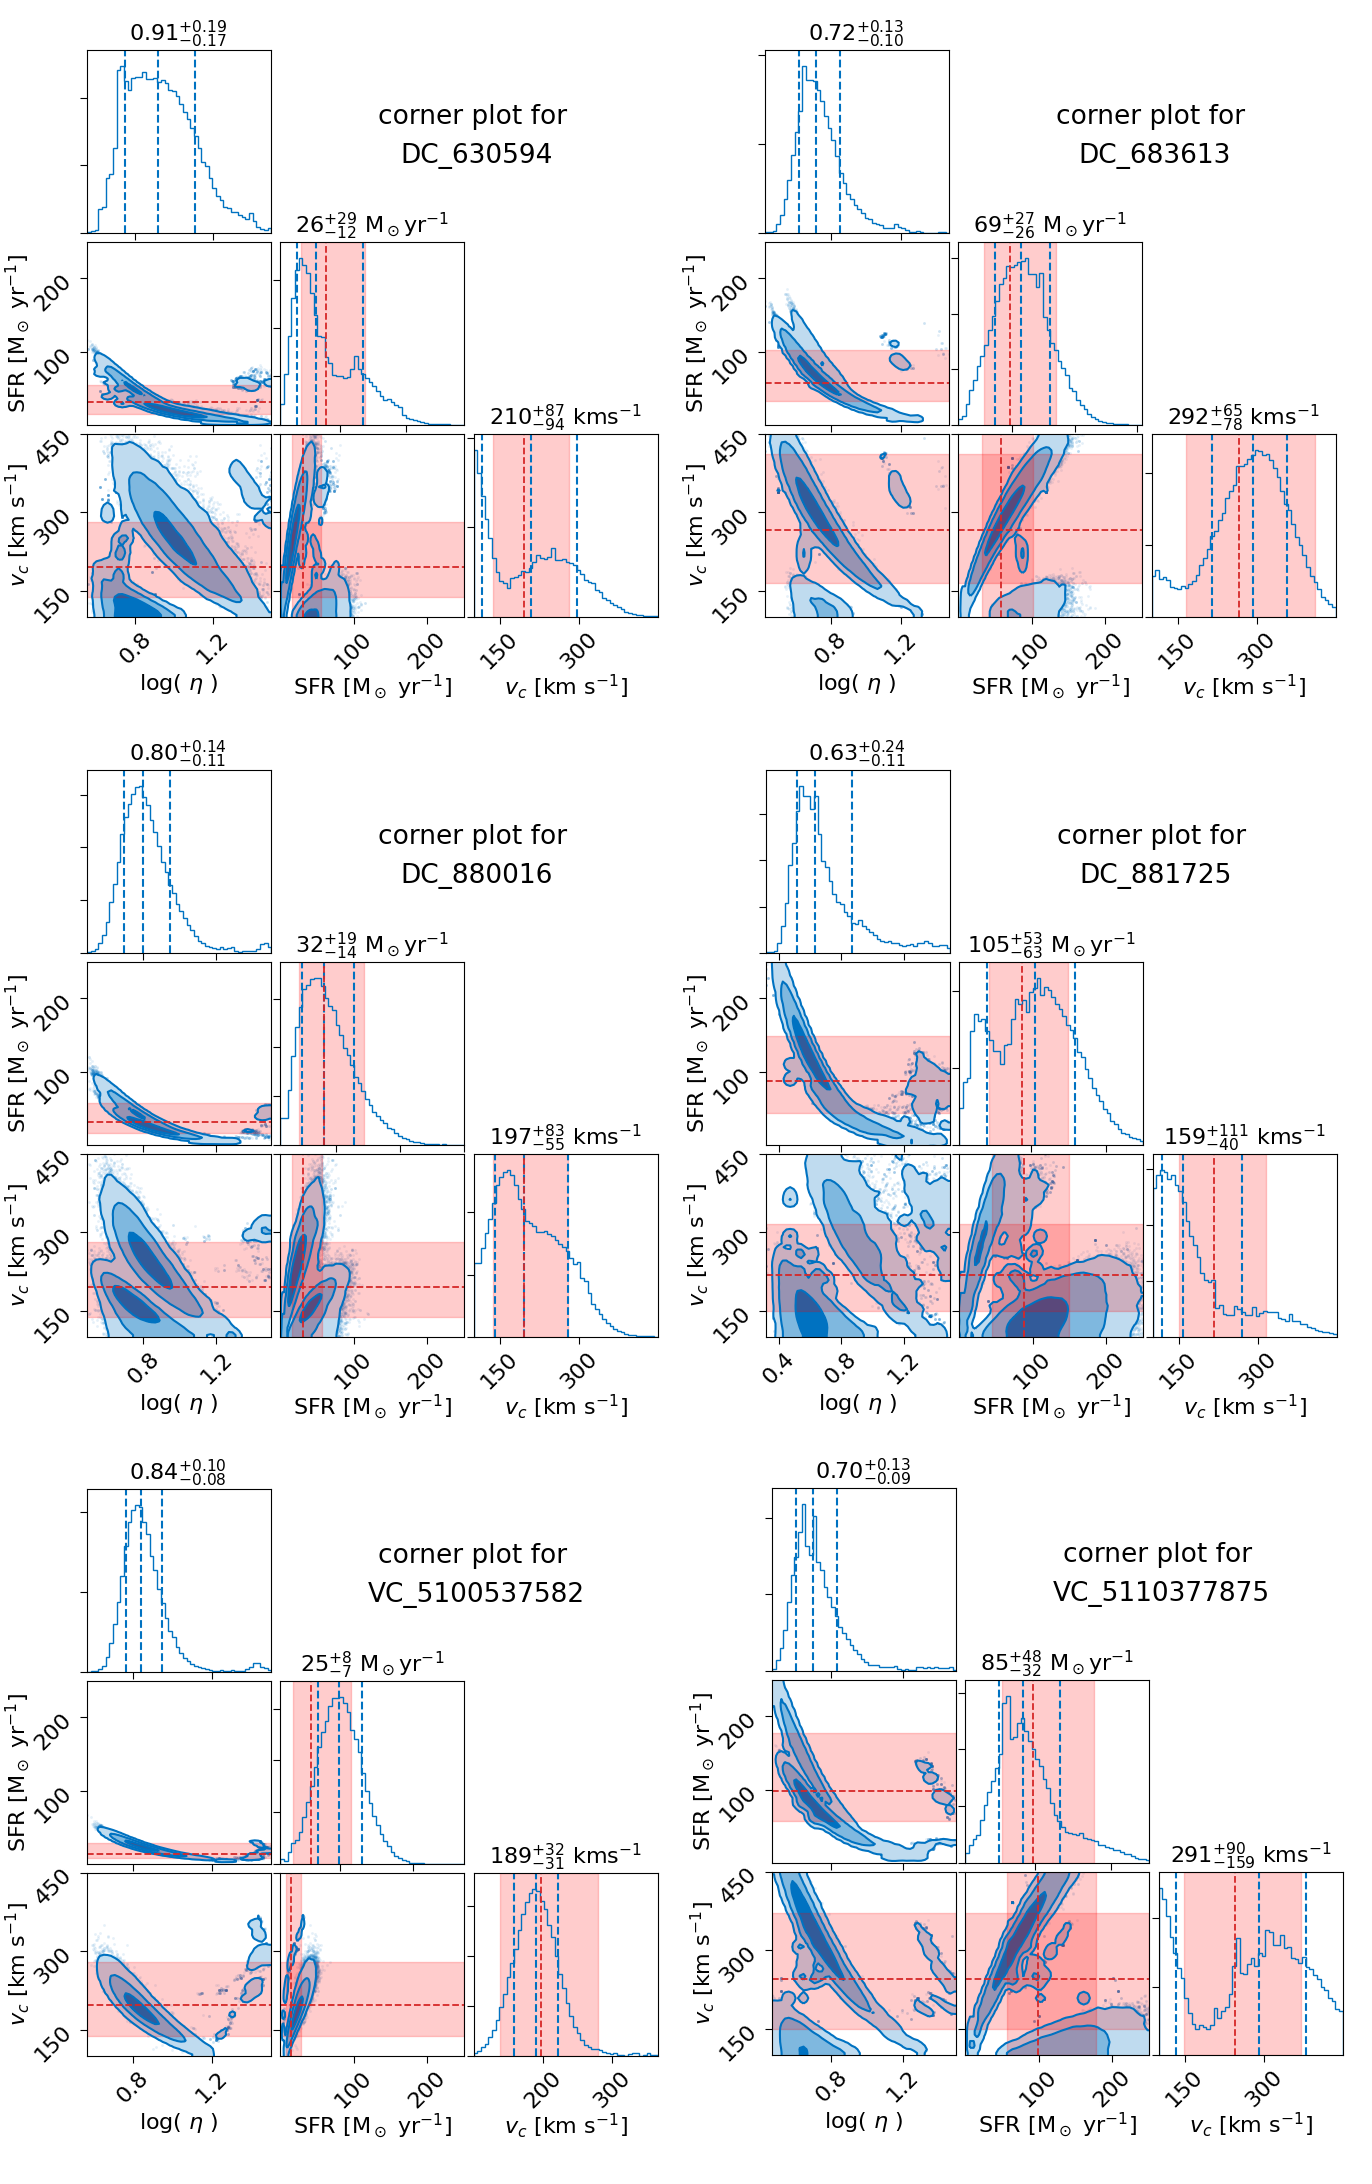
\includegraphics[width=1.0\textwidth]{plots/corner_final_2.png}
    \caption{Same as figure \ref{fig:corner_1}; the results for the rest of the data sample considered are shown here. 
    \label{fig:corner_2}
    }
\end{figure*}


\chapter{Conclusions and future outlook}
\vspace{20pt}
\label{chap:conclusion}



\vspace{13pt}


In this thesis work, we have argued that the recently discovered, very extended ($\approx 10-15\,\mathrm{kpc}$) \CII emitting halos around EoR galaxies are the result of supernova-driven cooling outflows. We have improved and extended the model presented in \citet{Pizzati20}, comparing its predictions with ALMA ALPINE observations of single systems at redshift $z\approx4-6$.

Having described the model and its results in detail, we are finally in the condition of giving some tentative answers to the compelling theoretical questions presented in section \ref{sec:theory_halos}:
\begin{itemize}
    \item Carbon is carried away from the center of galaxies (where it is produced by stellar nucleosynthesis) by hot modes of SF-driven winds. Energy and mass injections from SNe activity cause the gas to leave the galaxy with velocities in the range $300-500\,\kms$. Subsequently, the gas is gradually slowed down by the gravitational potential of the dark matter halo until it reaches a complete stop at radii $r\approx 10-15\,\mathrm{kpc}$. Thanks to this, we recover halos with finite sizes and masses around $M\approx 10^9\,\msun$.
    \item The success of the model largely relies on the fact that we follow precisely the catastrophic cooling of the outflow occurring within the central kpc. We find that cooling takes place for conditions (gas density $n\approx 1 \,\mathrm{cm}^{-3}$, temperature $T\approx 10^6\,\mathrm{K}$) consistent with the ones found by previous models and simulations \citep{Thompson16, Scannapieco:2017, gray2019catastrophic, danehkar_2021, fielding2021}. The gas cools very rapidly to $T \approx {\rm few} \times 100$ K, at the same time recombining. In this regime, the formation and survival of \CIIion ions are indeed possible. 
    \item We find that the outflow in our model is mostly neutral. This is because we assume that the escape fraction of ionizing radiation from the galaxy is negligible: thus, for the conditions of density and temperature in the outflow, hydrogen stays in the form of \HI, while carbon is collisionally ionized to \CIIion. The UV background radiation from other stars and quasars has indeed an effect on the gas, especially in the external low-density region. However, this does not prevent carbon to retain a significant abundance of \CIIion ions. 
    \item CMB suppression acts on the \CII emission by depleting the original \CII flux of factors between $2$ and $5$. Nevertheless, even accounting for this suppression effect we are able to recover the observed \CII luminosity ($L_\mathrm{CII}\approx 5-15\times10^8\,\mathrm{L}_\odot$).
    \item  Using our framework, we can infer crucial information on early galaxies, such as the outflow mass loading factor and the escape fraction of ionizing photons, that are hardly recovered from alternative methods at high redshifts. 
    \\By comparing our model predictions with observational data of individual ALPINE galaxies, we conclude that outflows are compatible with observations for values of the star formation rates and halo masses that lie in the range measured by pan-chromatic surveys.
    \\From this comparison, we infer values of the mass loading factor between $\eta\approx3$ and $\eta\approx10$, with inverse power-law dependences both on the stellar mass and on the star formation rate. Finally, we predict that a very low ionizing escape fraction from the parent galaxy is required ($\fesc \ll 1$). Values of $\fesc \gsim 0.2$, as those assumed by some reionization models, produce halo UV fields that are too intense for \CII to survive photoionization. 
\end{itemize} 

In brief, with our model, we can explain \CII halos as the result of cold neutral outflows from galaxies. Remarkably, although independent hydrodynamical simulations \citep{pallottini2017b, Arata:2019} have successfully matched both the dust and stellar continuum profiles deduced from observations \citep{Fujimoto19}, the same simulations could not reproduce the extended \CII line emission. This might be due to incomplete treatment of stellar feedback, or to numerical resolution issues related to the outflow catastrophic cooling. Our simple model, instead, can match the observed surface brightness. Hence, insight can be likely gained from a detailed comparison with simulations.

Alternatively, the failure of the simulations might indicate that the additional energy input required to transport the gas at such large distances could be provided by an AGN. This is suggested also by the values of the mass loading factor $\eta$ that we obtain from our analysis. These values are only marginally consistent with other measurements from starburst-driven outflows \citep{muratov2015, zhang2021empirical}, but they seem to be more compatible with the presence of AGN activity \citep[e.g.,][]{Fiore_2017}. This hypothesis must be tested via dedicated hydrodynamical simulations including radiative transfer.

The fact that the extended \CII halos surface brightness can be successfully fit by our model does not guarantee that outflows are the only possible explanation. Alternative interpretations, such as the presence of satellites, also need to be carefully explored. This is especially appropriate considering that, despite its success, the model presented here contains several limitations and hypotheses that will need to be further refined in the future:
\begin{itemize}
    \item The present one-dimensional treatment should be augmented with a full 3D numerical simulation of the outflow, also dropping the steady-state assumption made here. In this way, it may be possible to recreate a more realistic environment where non-spherical, truly multi-phase, outflows are launched by localized injection sites \citep{schneider2018production}. A similar picture is the one emerging from observations of the CGM local and high-redshift galaxies (chapter \ref{chap:halos}): outflows are often (bi-)conical-shaped, with different phases being characterized by different structures and morphologies. 
    \item A more realistic treatment of the circumgalactic/IGM environments is also necessary. Simulations show that accounting for an external CGM pressure might result in the formation of shocks in the outflowing gas \citep{samui:2008, Lochaas:2020, gray2019catastrophic}. Although we do not expect these shocks to dramatically affect the derived overall outflow structure, the detailed profile and extension of the \CII emitting region might turn out quantitatively different. This can be tested with less idealized, 3D models.
    \item Non-equilibrium cooling/recombination effects should also be considered when computing ionic abundances. In fact, several studies \citep[e.g.,][]{oppenheimer&schaye} have shown that assuming statistical equilibrium is generally not fair in very low-density environments illuminated by UV radiation.
\end{itemize}

%A first step towards an improvement of the model here considered is new parameters . 

Although some of these improvements might affect the quantitative conclusions of this work, it appears that so far outflows remain the best hypothesis to explain the puzzling nature of extended \CII halos. The role of outflows in extended halos formation could be tested in the future via dedicated ALMA observations. If so, we may be able to identify the smoking gun of the process by which the intergalactic medium was enriched with heavy elements during the EoR, taking another step forward in our understanding of the galaxy formation and evolution processes. 

%as witnessed by quasar absorption line experiments \citep{Dodorico13, Meyer19, Becker19}.


\chapter{Acknowledgements}
\vspace{20pt}
\label{chap:acknowledgements}



First of all, I am deeply grateful to Andrea Ferrara, who has been my supervisor and mentor for the last three years. His help, teaching, and advice have been invaluable to me. I first met him when I did not know anything about research, and since then, he has never stopped conducting me on the path to becoming a scientist. A huge thank you also to my co-supervisor, Andrea Pallottini. He helped me a lot with the project, and I could always rely on him to assist me and answer my numerous questions. In addition, my sincere gratitude goes to my internal supervisor, Michele Cignoni, for his precious feedback on my work and insightful comments on the very first draft of this document. 

\vspace{0.5cm}
This thesis work develops from a project that has started more than two years ago. In this project, I was helped and advised by several people: Simona Gallerani, Livia Vallini, Davide Decataldo, and Seiji Fujimoto. In particular, I want to thank Davide for helping me implement the cooling function, and Seiji, for sharing his study of the ALPINE \CII emission profiles. 


\vspace{0.5cm}
Being part of the Cosmology Group at SNS, even just for a few months, was one of the best parts of this project. This is because of the people I had the pleasure to meet there. I want to mention my office mates, Lorenzo and Daniele, and the other Ph.D. students here in the group, especially Ivan, David, Laura, and Zip. Thanks for all the meals and the coffee breaks we spent together.


\vspace{0.5cm}
To me, this thesis work is not just the ending of a project. It is also the ending of a five-year experience in Pisa. For this reason, I want to take this opportunity to say thank you to the people I have shared this journey with: my class at SNS, and all the friends I have met at SNS and UniPi. They are too many to be listed here, but it's only because of them if I feel utterly grateful for the time spent here in Pisa. A special thanks to Beppe, for reading this thesis; to my flatmates Marco, Massimo, Federico, Lavinia, and Margherita, for the time shared, especially during the lockdown; and to Seyma, for accepting my poor judgment in hiking trips, and for giving me a reason to graduate on time.


\vspace{0.5cm}
My final thanks go to my family: my parents, siblings, grandparents, aunts, uncles, and cousins. Most of all, I want to thank my parents, Enrica and Carlo. Their advice, constant support, and unconditional love have been essential to me even in these years spent far from home. 



\bibliography{biblio}


\end{document}